\documentclass[twoside]{book}

% Packages required by doxygen
\usepackage{calc}
\usepackage{doxygen}
\usepackage{graphicx}
\usepackage[utf8]{inputenc}
\usepackage{makeidx}
\usepackage{multicol}
\usepackage{multirow}
\usepackage{textcomp}
\usepackage[table]{xcolor}

% Font selection
\usepackage[T1]{fontenc}
\usepackage{mathptmx}
\usepackage[scaled=.90]{helvet}
\usepackage{courier}
\usepackage{amssymb}
\usepackage{sectsty}
\renewcommand{\familydefault}{\sfdefault}
\allsectionsfont{%
  \fontseries{bc}\selectfont%
  \color{darkgray}%
}
\renewcommand{\DoxyLabelFont}{%
  \fontseries{bc}\selectfont%
  \color{darkgray}%
}

% Page & text layout
\usepackage{geometry}
\geometry{%
  a4paper,%
  top=2.5cm,%
  bottom=2.5cm,%
  left=2.5cm,%
  right=2.5cm%
}
\tolerance=750
\hfuzz=15pt
\hbadness=750
\setlength{\emergencystretch}{15pt}
\setlength{\parindent}{0cm}
\setlength{\parskip}{0.2cm}
\makeatletter
\renewcommand{\paragraph}{%
  \@startsection{paragraph}{4}{0ex}{-1.0ex}{1.0ex}{%
    \normalfont\normalsize\bfseries\SS@parafont%
  }%
}
\renewcommand{\subparagraph}{%
  \@startsection{subparagraph}{5}{0ex}{-1.0ex}{1.0ex}{%
    \normalfont\normalsize\bfseries\SS@subparafont%
  }%
}
\makeatother

% Headers & footers
\usepackage{fancyhdr}
\pagestyle{fancyplain}
\fancyhead[LE]{\fancyplain{}{\bfseries\thepage}}
\fancyhead[CE]{\fancyplain{}{}}
\fancyhead[RE]{\fancyplain{}{\bfseries\leftmark}}
\fancyhead[LO]{\fancyplain{}{\bfseries\rightmark}}
\fancyhead[CO]{\fancyplain{}{}}
\fancyhead[RO]{\fancyplain{}{\bfseries\thepage}}
\fancyfoot[LE]{\fancyplain{}{}}
\fancyfoot[CE]{\fancyplain{}{}}
\fancyfoot[RE]{\fancyplain{}{\bfseries\scriptsize Generated on Thu May 4 2017 21\-:51\-:09 for v\-Renderer -\/ Path tracer by Doxygen }}
\fancyfoot[LO]{\fancyplain{}{\bfseries\scriptsize Generated on Thu May 4 2017 21\-:51\-:09 for v\-Renderer -\/ Path tracer by Doxygen }}
\fancyfoot[CO]{\fancyplain{}{}}
\fancyfoot[RO]{\fancyplain{}{}}
\renewcommand{\footrulewidth}{0.4pt}
\renewcommand{\chaptermark}[1]{%
  \markboth{#1}{}%
}
\renewcommand{\sectionmark}[1]{%
  \markright{\thesection\ #1}%
}

% Indices & bibliography
\usepackage{natbib}
\usepackage[titles]{tocloft}
\setcounter{tocdepth}{3}
\setcounter{secnumdepth}{5}
\makeindex

% Hyperlinks (required, but should be loaded last)
\usepackage{ifpdf}
\ifpdf
  \usepackage[pdftex,pagebackref=true]{hyperref}
\else
  \usepackage[ps2pdf,pagebackref=true]{hyperref}
\fi
\hypersetup{%
  colorlinks=true,%
  linkcolor=blue,%
  citecolor=blue,%
  unicode%
}

% Custom commands
\newcommand{\clearemptydoublepage}{%
  \newpage{\pagestyle{empty}\cleardoublepage}%
}


%===== C O N T E N T S =====

\begin{document}

% Titlepage & ToC
\hypersetup{pageanchor=false}
\pagenumbering{roman}
\begin{titlepage}
\vspace*{7cm}
\begin{center}%
{\Large v\-Renderer -\/ Path tracer }\\
\vspace*{1cm}
{\large Generated by Doxygen 1.8.5}\\
\vspace*{0.5cm}
{\small Thu May 4 2017 21:51:09}\\
\end{center}
\end{titlepage}
\clearemptydoublepage
\tableofcontents
\clearemptydoublepage
\pagenumbering{arabic}
\hypersetup{pageanchor=true}

%--- Begin generated contents ---
\chapter{Todo List}
\label{todo}
\hypertarget{todo}{}

\begin{DoxyRefList}
\item[\label{todo__todo000005}%
\hypertarget{todo__todo000005}{}%
File \hyperlink{AABB_8h}{A\-A\-B\-B.h} ]-\/  
\item[\label{todo__todo000006}%
\hypertarget{todo__todo000006}{}%
File \hyperlink{BRDFLoader_8h}{B\-R\-D\-F\-Loader.h} ]Use the double data instead  
\item[\label{todo__todo000007}%
\hypertarget{todo__todo000007}{}%
File \hyperlink{BVHNodes_8h}{B\-V\-H\-Nodes.h} ]-\/  
\item[\label{todo__todo000008}%
\hypertarget{todo__todo000008}{}%
File \hyperlink{Camera_8h}{Camera.h} ]Implement the \char`\"{}\-A Realistic Camera Model for Computer Graphics\char`\"{} described at \href{http://www.cs.virginia.edu/~gfx/courses/2003/ImageSynthesis/papers/Cameras/Realistic%20Camera%20Model.pdf}{\tt http\-://www.\-cs.\-virginia.\-edu/$\sim$gfx/courses/2003/\-Image\-Synthesis/papers/\-Cameras/\-Realistic\%20\-Camera\%20\-Model.\-pdf}  
\item[\label{todo__todo000002}%
\hypertarget{todo__todo000002}{}%
File \hyperlink{MathHelpers_8cuh}{Math\-Helpers.cuh} ]-\/  
\item[\label{todo__todo000010}%
\hypertarget{todo__todo000010}{}%
File \hyperlink{MeshLoader_8h}{Mesh\-Loader.h} ]Allow the loading of more than a single model  
\item[\label{todo__todo000011}%
\hypertarget{todo__todo000011}{}%
File \hyperlink{NGLScene_8h}{N\-G\-L\-Scene.h} ]General cleanup and move the pass through slots from the scene to the renderer Switch to Open\-Image\-I\-O for H\-D\-R\-I and texture loading. Bring in colour management options with Open\-Color\-I\-O  
\item[\label{todo__todo000003}%
\hypertarget{todo__todo000003}{}%
File \hyperlink{PathTracer_8cuh}{Path\-Tracer.cuh} ]-\/  
\item[\label{todo__todo000001}%
\hypertarget{todo__todo000001}{}%
File \hyperlink{PathTracer_8h}{Path\-Tracer.h} ]-\/  
\item[\label{todo__todo000004}%
\hypertarget{todo__todo000004}{}%
File \hyperlink{RayIntersection_8cuh}{Ray\-Intersection.cuh} ]-\/  
\item[\label{todo__todo000012}%
\hypertarget{todo__todo000012}{}%
File \hyperlink{SBVH_8h}{S\-B\-V\-H.h} ]-\/  
\item[\label{todo__todo000009}%
\hypertarget{todo__todo000009}{}%
Namespace \hyperlink{namespaceUi}{Ui} ]Fix scene tree, U\-I styling  
\item[\label{todo__todo000014}%
\hypertarget{todo__todo000014}{}%
File \hyperlink{vDataTypes_8h}{v\-Data\-Types.h} ]-\/  
\item[\label{todo__todo000015}%
\hypertarget{todo__todo000015}{}%
File \hyperlink{vRenderer_8h}{v\-Renderer.h} ]-\/  
\item[\label{todo__todo000016}%
\hypertarget{todo__todo000016}{}%
File \hyperlink{vRendererCL_8h}{v\-Renderer\-C\-L.h} ]Implement the depth buffer for Open\-C\-L and make sure cleanup is done correctly, especially when overwriting existing buffers  
\item[\label{todo__todo000017}%
\hypertarget{todo__todo000017}{}%
File \hyperlink{vRendererCuda_8h}{v\-Renderer\-Cuda.h} ]-\/ 
\end{DoxyRefList}
\chapter{Namespace Index}
\section{Namespace List}
Here is a list of all documented namespaces with brief descriptions\-:\begin{DoxyCompactList}
\item\contentsline{section}{\hyperlink{namespaceUi}{Ui} \\*Main window encapsulating the U\-I and output window }{\pageref{namespaceUi}}{}
\item\contentsline{section}{\hyperlink{namespacevUtilities}{v\-Utilities} \\*Utility namespace }{\pageref{namespacevUtilities}}{}
\end{DoxyCompactList}

\chapter{Hierarchical Index}
\section{Class Hierarchy}
This inheritance list is sorted roughly, but not completely, alphabetically\-:\begin{DoxyCompactList}
\item \contentsline{section}{A\-A\-B\-B}{\pageref{classAABB}}{}
\item \contentsline{section}{B\-V\-H\-Node}{\pageref{classBVHNode}}{}
\begin{DoxyCompactList}
\item \contentsline{section}{Inner\-Node}{\pageref{classInnerNode}}{}
\item \contentsline{section}{Leaf\-Node}{\pageref{classLeafNode}}{}
\end{DoxyCompactList}
\item \contentsline{section}{Camera}{\pageref{classCamera}}{}
\item \contentsline{section}{mat4}{\pageref{structmat4}}{}
\item Q\-Main\-Window\begin{DoxyCompactList}
\item \contentsline{section}{Main\-Window}{\pageref{classMainWindow}}{}
\end{DoxyCompactList}
\item Q\-Open\-G\-L\-Widget\begin{DoxyCompactList}
\item \contentsline{section}{N\-G\-L\-Scene}{\pageref{classNGLScene}}{}
\end{DoxyCompactList}
\item \contentsline{section}{qt\-\_\-meta\-\_\-stringdata\-\_\-\-Main\-Window\-\_\-t}{\pageref{structqt__meta__stringdata__MainWindow__t}}{}
\item \contentsline{section}{qt\-\_\-meta\-\_\-stringdata\-\_\-\-N\-G\-L\-Scene\-\_\-t}{\pageref{structqt__meta__stringdata__NGLScene__t}}{}
\item \contentsline{section}{Ray}{\pageref{structRay}}{}
\item \contentsline{section}{S\-B\-V\-H}{\pageref{classSBVH}}{}
\item \contentsline{section}{Sphere}{\pageref{structSphere}}{}
\item \contentsline{section}{Ui\-\_\-\-Main\-Window}{\pageref{classUi__MainWindow}}{}
\begin{DoxyCompactList}
\item \contentsline{section}{Ui\-:\-:Main\-Window}{\pageref{classUi_1_1MainWindow}}{}
\end{DoxyCompactList}
\item \contentsline{section}{v\-B\-R\-D\-F\-Loader}{\pageref{classvBRDFLoader}}{}
\item \contentsline{section}{v\-Camera}{\pageref{structvCamera}}{}
\item \contentsline{section}{v\-Hit\-Data}{\pageref{structvHitData}}{}
\item \contentsline{section}{v\-H\-Triangle}{\pageref{structvHTriangle}}{}
\item \contentsline{section}{v\-H\-Vert}{\pageref{structvHVert}}{}
\item \contentsline{section}{v\-Mesh\-Data}{\pageref{structvMeshData}}{}
\item \contentsline{section}{v\-Mesh\-Loader}{\pageref{classvMeshLoader}}{}
\item \contentsline{section}{v\-Renderer}{\pageref{classvRenderer}}{}
\begin{DoxyCompactList}
\item \contentsline{section}{v\-Renderer\-C\-L}{\pageref{classvRendererCL}}{}
\item \contentsline{section}{v\-Renderer\-Cuda}{\pageref{classvRendererCuda}}{}
\end{DoxyCompactList}
\item \contentsline{section}{Win\-Params}{\pageref{structWinParams}}{}
\end{DoxyCompactList}

\chapter{Class Index}
\section{Class List}
Here are the classes, structs, unions and interfaces with brief descriptions\-:\begin{DoxyCompactList}
\item\contentsline{section}{\hyperlink{classAABB}{A\-A\-B\-B} \\*The \hyperlink{classAABB}{A\-A\-B\-B} class, encapsulates a simple \hyperlink{classAABB}{A\-A\-B\-B} class to be used with building the acceleration structure for the path tracer }{\pageref{classAABB}}{}
\item\contentsline{section}{\hyperlink{classBVHNode}{B\-V\-H\-Node} \\*Abstract base class for the nodes }{\pageref{classBVHNode}}{}
\item\contentsline{section}{\hyperlink{classCamera}{Camera} \\*Simple camera class that handles movement and rotations, also keeps track whether the camera is dirty e.\-g. if the renderer needs to clear its buffers and start tracing from the beginning }{\pageref{classCamera}}{}
\item\contentsline{section}{\hyperlink{classInnerNode}{Inner\-Node} \\*Inner node, e.\-g. a node with children }{\pageref{classInnerNode}}{}
\item\contentsline{section}{\hyperlink{classLeafNode}{Leaf\-Node} \\*Simple leaf node class, stores indices to triangles inside the node }{\pageref{classLeafNode}}{}
\item\contentsline{section}{\hyperlink{classUi_1_1MainWindow}{Ui\-::\-Main\-Window} }{\pageref{classUi_1_1MainWindow}}{}
\item\contentsline{section}{\hyperlink{classMainWindow}{Main\-Window} \\*The \hyperlink{classMainWindow}{Main\-Window} class }{\pageref{classMainWindow}}{}
\item\contentsline{section}{\hyperlink{structmat4}{mat4} \\*Simple \hyperlink{structmat4}{mat4} struct used for normal map calculations }{\pageref{structmat4}}{}
\item\contentsline{section}{\hyperlink{classNGLScene}{N\-G\-L\-Scene} \\*Our main glwindow widget for N\-G\-L applications all drawing elements are put in this file }{\pageref{classNGLScene}}{}
\item\contentsline{section}{\hyperlink{structqt__meta__stringdata__MainWindow__t}{qt\-\_\-meta\-\_\-stringdata\-\_\-\-Main\-Window\-\_\-t} }{\pageref{structqt__meta__stringdata__MainWindow__t}}{}
\item\contentsline{section}{\hyperlink{structqt__meta__stringdata__NGLScene__t}{qt\-\_\-meta\-\_\-stringdata\-\_\-\-N\-G\-L\-Scene\-\_\-t} }{\pageref{structqt__meta__stringdata__NGLScene__t}}{}
\item\contentsline{section}{\hyperlink{structRay}{Ray} \\*\hyperlink{structRay}{Ray} Simple structure for a ray }{\pageref{structRay}}{}
\item\contentsline{section}{\hyperlink{classSBVH}{S\-B\-V\-H} \\*The class builds the acceleration structure when given a vector of triangles and vertices }{\pageref{classSBVH}}{}
\item\contentsline{section}{\hyperlink{structSphere}{Sphere} \\*\hyperlink{structSphere}{Sphere} Simple sphere structure, used for the example sphere, cornell box scene and few others }{\pageref{structSphere}}{}
\item\contentsline{section}{\hyperlink{classUi__MainWindow}{Ui\-\_\-\-Main\-Window} }{\pageref{classUi__MainWindow}}{}
\item\contentsline{section}{\hyperlink{classvBRDFLoader}{v\-B\-R\-D\-F\-Loader} \\*Currently only handles simple loading of the brdf binary data }{\pageref{classvBRDFLoader}}{}
\item\contentsline{section}{\hyperlink{structvCamera}{v\-Camera} \\*V\-Camera Simple structure to hold the camera on the G\-P\-U }{\pageref{structvCamera}}{}
\item\contentsline{section}{\hyperlink{structvHitData}{v\-Hit\-Data} \\*V\-Hit\-Data Simple structure to contain the details of a ray intersection }{\pageref{structvHitData}}{}
\item\contentsline{section}{\hyperlink{structvHTriangle}{v\-H\-Triangle} \\*V\-H\-Triangle Simple triangle structure containing the vertex indices of a triangle, used to contain normal and other triangle specific data }{\pageref{structvHTriangle}}{}
\item\contentsline{section}{\hyperlink{structvHVert}{v\-H\-Vert} \\*V\-H\-Vert Simple vertex structure, contains the position, normal, tangent and uv-\/coordinates of a vertex }{\pageref{structvHVert}}{}
\item\contentsline{section}{\hyperlink{structvMeshData}{v\-Mesh\-Data} \\*Simple structure to hold the data needed by the G\-P\-U }{\pageref{structvMeshData}}{}
\item\contentsline{section}{\hyperlink{classvMeshLoader}{v\-Mesh\-Loader} \\*Mesh loader class that reads in a 3d model using assimp and generates the \hyperlink{classSBVH}{S\-B\-V\-H} acceleration structure }{\pageref{classvMeshLoader}}{}
\item\contentsline{section}{\hyperlink{classvRenderer}{v\-Renderer} \\*Abstract base class for the path tracer }{\pageref{classvRenderer}}{}
\item\contentsline{section}{\hyperlink{classvRendererCL}{v\-Renderer\-C\-L} \\*Open\-C\-L implementation of the renderer }{\pageref{classvRendererCL}}{}
\item\contentsline{section}{\hyperlink{classvRendererCuda}{v\-Renderer\-Cuda} \\*Cuda implementation of the renderer }{\pageref{classvRendererCuda}}{}
\item\contentsline{section}{\hyperlink{structWinParams}{Win\-Params} }{\pageref{structWinParams}}{}
\end{DoxyCompactList}

\chapter{File Index}
\section{File List}
Here is a list of all documented files with brief descriptions\-:\begin{DoxyCompactList}
\item\contentsline{section}{{\bfseries ui\-\_\-mainwindow.\-h} }{\pageref{ui__mainwindow_8h}}{}
\item\contentsline{section}{cl/include/\hyperlink{PathTracer_8h}{Path\-Tracer.\-h} \\*Open\-C\-L device path tracer function definitions and structs }{\pageref{PathTracer_8h}}{}
\item\contentsline{section}{cl/include/{\bfseries Ray\-Intersection.\-h} }{\pageref{RayIntersection_8h}}{}
\item\contentsline{section}{cl/include/{\bfseries Utilities.\-h} }{\pageref{cl_2include_2Utilities_8h}}{}
\item\contentsline{section}{cl/src/\hyperlink{PathTracer_8cl}{Path\-Tracer.\-cl} \\*Device (Open\-C\-L) implementation of the path tracer. As the implementation is pretty much the same as the Cuda one. The documentation for most everything can be found under the cuda docs }{\pageref{PathTracer_8cl}}{}
\item\contentsline{section}{cuda/include/\hyperlink{MathHelpers_8cuh}{Math\-Helpers.\-cuh} \\*Device math helper functions }{\pageref{MathHelpers_8cuh}}{}
\item\contentsline{section}{cuda/include/\hyperlink{PathTracer_8cuh}{Path\-Tracer.\-cuh} \\*C\-P\-U-\/\-G\-P\-U header file for the path tracer }{\pageref{PathTracer_8cuh}}{}
\item\contentsline{section}{cuda/include/\hyperlink{RayIntersection_8cuh}{Ray\-Intersection.\-cuh} \\*Ray-\/\-X\-X intersection functions }{\pageref{RayIntersection_8cuh}}{}
\item\contentsline{section}{cuda/src/\hyperlink{PathTracer_8cu}{Path\-Tracer.\-cu} \\*Device (cuda) implementation of the path tracer }{\pageref{PathTracer_8cu}}{}
\item\contentsline{section}{include/\hyperlink{AABB_8h}{A\-A\-B\-B.\-h} \\*Simple \hyperlink{classAABB}{A\-A\-B\-B} used with the \hyperlink{classSBVH}{S\-B\-V\-H} }{\pageref{AABB_8h}}{}
\item\contentsline{section}{include/\hyperlink{BRDFLoader_8h}{B\-R\-D\-F\-Loader.\-h} \\*Loads M\-E\-R\-L B\-R\-D\-F binary data to R\-B\-G format. Data loading from the binary is based on the M\-E\-R\-L 100 code available at \href{http://people.csail.mit.edu/wojciech/BRDFDatabase/code/BRDFRead.cpp}{\tt http\-://people.\-csail.\-mit.\-edu/wojciech/\-B\-R\-D\-F\-Database/code/\-B\-R\-D\-F\-Read.\-cpp} }{\pageref{BRDFLoader_8h}}{}
\item\contentsline{section}{include/\hyperlink{BVHNodes_8h}{B\-V\-H\-Nodes.\-h} \\*Simple node class(es) for the \hyperlink{classSBVH}{S\-B\-V\-H} tree }{\pageref{BVHNodes_8h}}{}
\item\contentsline{section}{include/\hyperlink{Camera_8h}{Camera.\-h} \\*Simple virtual camera class used in the scene }{\pageref{Camera_8h}}{}
\item\contentsline{section}{include/{\bfseries mainwindow.\-h} }{\pageref{mainwindow_8h}}{}
\item\contentsline{section}{include/\hyperlink{MeshLoader_8h}{Mesh\-Loader.\-h} \\*Simple mesh loader, uses Assimp to load in a 3d model and passes the data to the \hyperlink{classSBVH}{S\-B\-V\-H} builder Finally returns the data to be passed to the G\-P\-U }{\pageref{MeshLoader_8h}}{}
\item\contentsline{section}{include/\hyperlink{NGLScene_8h}{N\-G\-L\-Scene.\-h} \\*This class inherits from the Qt Open\-G\-L\-Window and allows us to use N\-G\-L to draw Open\-G\-L Creates the renderer, handles data propagation from the U\-I to the renderer and creates Open\-G\-L textures and V\-B\-O's to visualise the renderer output }{\pageref{NGLScene_8h}}{}
\item\contentsline{section}{include/\hyperlink{SBVH_8h}{S\-B\-V\-H.\-h} \\*\hyperlink{classSBVH}{S\-B\-V\-H} class encapsulating the building of a Spatial Splits in Bounding Volume Hierarchies acceleration structure. \hyperlink{classSBVH}{S\-B\-V\-H} aims to minimise the node intersections of a regular B\-V\-H. The implementation is based on \char`\"{}\-Spatial Splits in Bounding Volume Hierarchies\char`\"{} by Martin Stitch et. al. Available at \href{http://www.nvidia.ca/docs/IO/77714/sbvh.pdf}{\tt http\-://www.\-nvidia.\-ca/docs/\-I\-O/77714/sbvh.\-pdf} }{\pageref{SBVH_8h}}{}
\item\contentsline{section}{include/{\bfseries Utilities.\-h} }{\pageref{include_2Utilities_8h}}{}
\item\contentsline{section}{include/\hyperlink{vDataTypes_8h}{v\-Data\-Types.\-h} \\*Simple data structures to hold the mesh (and other) data on the C\-P\-U }{\pageref{vDataTypes_8h}}{}
\item\contentsline{section}{include/\hyperlink{vRenderer_8h}{v\-Renderer.\-h} \\*Abstract base class for the renderer }{\pageref{vRenderer_8h}}{}
\item\contentsline{section}{include/\hyperlink{vRendererCL_8h}{v\-Renderer\-C\-L.\-h} \\*Open\-C\-L implementation of the renderer }{\pageref{vRendererCL_8h}}{}
\item\contentsline{section}{include/\hyperlink{vRendererCuda_8h}{v\-Renderer\-Cuda.\-h} \\*Cuda implementation of the renderer }{\pageref{vRendererCuda_8h}}{}
\item\contentsline{section}{include/{\bfseries Window\-Params.\-h} }{\pageref{WindowParams_8h}}{}
\item\contentsline{section}{src/\hyperlink{BRDFLoader_8cpp}{B\-R\-D\-F\-Loader.\-cpp} \\*Loads M\-E\-R\-L B\-R\-D\-F binary data }{\pageref{BRDFLoader_8cpp}}{}
\item\contentsline{section}{src/\hyperlink{BVHNodes_8cpp}{B\-V\-H\-Nodes.\-cpp} \\*Nodes/node methods used in the \hyperlink{classSBVH}{S\-B\-V\-H} }{\pageref{BVHNodes_8cpp}}{}
\item\contentsline{section}{src/\hyperlink{Camera_8cpp}{Camera.\-cpp} \\*Implements the \hyperlink{classCamera}{Camera} class }{\pageref{Camera_8cpp}}{}
\item\contentsline{section}{src/\hyperlink{MeshLoader_8cpp}{Mesh\-Loader.\-cpp} \\*Loads 3\-D models using Assimp }{\pageref{MeshLoader_8cpp}}{}
\item\contentsline{section}{src/\hyperlink{NGLScene_8cpp}{N\-G\-L\-Scene.\-cpp} \\*Implements the \hyperlink{classNGLScene}{N\-G\-L\-Scene}, Open\-G\-L and Cuda/\-Open\-C\-L interop etc }{\pageref{NGLScene_8cpp}}{}
\item\contentsline{section}{src/\hyperlink{vRendererCL_8cpp}{v\-Renderer\-C\-L.\-cpp} \\*Implements the Open\-C\-L version of the renderer }{\pageref{vRendererCL_8cpp}}{}
\item\contentsline{section}{src/\hyperlink{vRendererCuda_8cpp}{v\-Renderer\-Cuda.\-cpp} \\*Implements the Cuda version of the renderer }{\pageref{vRendererCuda_8cpp}}{}
\end{DoxyCompactList}

\chapter{Namespace Documentation}
\hypertarget{namespaceUi}{\section{Ui Namespace Reference}
\label{namespaceUi}\index{Ui@{Ui}}
}


Main window encapsulating the U\-I and output window.  


\subsection*{Classes}
\begin{DoxyCompactItemize}
\item 
class \hyperlink{classUi_1_1MainWindow}{Main\-Window}
\end{DoxyCompactItemize}


\subsection{Detailed Description}
Main window encapsulating the U\-I and output window. \begin{DoxyAuthor}{Author}
Teemu Lindborg 
\end{DoxyAuthor}
\begin{DoxyVersion}{Version}
1.\-0 
\end{DoxyVersion}
\begin{DoxyDate}{Date}
04/05/17 Updated to N\-C\-C\-A Coding standard Revision History \-: Initial Version 08/12/16 
\end{DoxyDate}
\begin{DoxyRefDesc}{Todo}
\item[\hyperlink{todo__todo000009}{Todo}]Fix scene tree, U\-I styling \end{DoxyRefDesc}

\hypertarget{namespacevUtilities}{\section{v\-Utilities Namespace Reference}
\label{namespacevUtilities}\index{v\-Utilities@{v\-Utilities}}
}


Utility namespace.  


\subsection*{Functions}
\begin{DoxyCompactItemize}
\item 
ngl\-::\-Vec3 \hyperlink{namespacevUtilities_aa7cc71c40bf034efd3a5834b2307a793}{min\-Vec3} (const ngl\-::\-Vec3 \&\-\_\-v1, const ngl\-::\-Vec3 \&\-\_\-v2)
\begin{DoxyCompactList}\small\item\em min\-Vec3 Get the component-\/wise minimums from two vectors \end{DoxyCompactList}\item 
ngl\-::\-Vec3 \hyperlink{namespacevUtilities_a8418b00f3f9e52b6f186b5e12ece8e15}{max\-Vec3} (const ngl\-::\-Vec3 \&\-\_\-v1, const ngl\-::\-Vec3 \&\-\_\-v2)
\begin{DoxyCompactList}\small\item\em max\-Vec3 Get the component-\/wise maximums from two vectors \end{DoxyCompactList}\item 
ngl\-::\-Vec3 \hyperlink{namespacevUtilities_adb4a633333be024bd738145162d53673}{lerp} (const ngl\-::\-Vec3 \&\-\_\-v1, const ngl\-::\-Vec3 \&\-\_\-v2, const float \&\-\_\-t)
\begin{DoxyCompactList}\small\item\em lerp Perform linear interpolation between two vectors given an alpha \end{DoxyCompactList}\item 
float \hyperlink{namespacevUtilities_a7e5df8352dd98340207816292e1ccfcf}{clamp} (const float \&\-\_\-v, const float \&\-\_\-min, const float \&\-\_\-max)
\begin{DoxyCompactList}\small\item\em clamp Clamps a given float between two values \end{DoxyCompactList}\item 
void \hyperlink{namespacevUtilities_a3828a1aa0cfbd068f42601e54f479359}{clamp\-Vec3} (ngl\-::\-Vec3 \&io\-\_\-v, const ngl\-::\-Vec3 \&\-\_\-low, const ngl\-::\-Vec3 \&\-\_\-high)
\begin{DoxyCompactList}\small\item\em clamp\-Vec3 Performs component-\/wise clamping for a vector \end{DoxyCompactList}\item 
{\footnotesize template$<$typename T $>$ }\\void \hyperlink{namespacevUtilities_a7e8796a2bff5498b31a9e0ad63199ac7}{swap} (T \&\-\_\-a, T \&\-\_\-b)
\begin{DoxyCompactList}\small\item\em swap Swaps two elements around \end{DoxyCompactList}\end{DoxyCompactItemize}


\subsection{Detailed Description}
Utility namespace. 

\subsection{Function Documentation}
\hypertarget{namespacevUtilities_a7e5df8352dd98340207816292e1ccfcf}{\index{v\-Utilities@{v\-Utilities}!clamp@{clamp}}
\index{clamp@{clamp}!vUtilities@{v\-Utilities}}
\subsubsection[{clamp}]{\setlength{\rightskip}{0pt plus 5cm}float v\-Utilities\-::clamp (
\begin{DoxyParamCaption}
\item[{const float \&}]{\-\_\-v, }
\item[{const float \&}]{\-\_\-min, }
\item[{const float \&}]{\-\_\-max}
\end{DoxyParamCaption}
)\hspace{0.3cm}{\ttfamily [inline]}}}\label{namespacevUtilities_a7e5df8352dd98340207816292e1ccfcf}


clamp Clamps a given float between two values 


\begin{DoxyParams}{Parameters}
{\em \-\_\-v} & Value to clamp \\
\hline
{\em \-\_\-min} & Minimum limit of the clamp \\
\hline
{\em \-\_\-max} & Maximum limit of the clamp \\
\hline
\end{DoxyParams}
\begin{DoxyReturn}{Returns}
Clamped value 
\end{DoxyReturn}
\hypertarget{namespacevUtilities_a3828a1aa0cfbd068f42601e54f479359}{\index{v\-Utilities@{v\-Utilities}!clamp\-Vec3@{clamp\-Vec3}}
\index{clamp\-Vec3@{clamp\-Vec3}!vUtilities@{v\-Utilities}}
\subsubsection[{clamp\-Vec3}]{\setlength{\rightskip}{0pt plus 5cm}void v\-Utilities\-::clamp\-Vec3 (
\begin{DoxyParamCaption}
\item[{ngl\-::\-Vec3 \&}]{io\-\_\-v, }
\item[{const ngl\-::\-Vec3 \&}]{\-\_\-low, }
\item[{const ngl\-::\-Vec3 \&}]{\-\_\-high}
\end{DoxyParamCaption}
)\hspace{0.3cm}{\ttfamily [inline]}}}\label{namespacevUtilities_a3828a1aa0cfbd068f42601e54f479359}


clamp\-Vec3 Performs component-\/wise clamping for a vector 


\begin{DoxyParams}{Parameters}
{\em io\-\_\-v} & Input vector to be clamped \\
\hline
{\em \-\_\-low} & Minimum limit of the clamp \\
\hline
{\em \-\_\-high} & Maximum limit of the clamp \\
\hline
\end{DoxyParams}
\hypertarget{namespacevUtilities_adb4a633333be024bd738145162d53673}{\index{v\-Utilities@{v\-Utilities}!lerp@{lerp}}
\index{lerp@{lerp}!vUtilities@{v\-Utilities}}
\subsubsection[{lerp}]{\setlength{\rightskip}{0pt plus 5cm}ngl\-::\-Vec3 v\-Utilities\-::lerp (
\begin{DoxyParamCaption}
\item[{const ngl\-::\-Vec3 \&}]{\-\_\-v1, }
\item[{const ngl\-::\-Vec3 \&}]{\-\_\-v2, }
\item[{const float \&}]{\-\_\-t}
\end{DoxyParamCaption}
)\hspace{0.3cm}{\ttfamily [inline]}}}\label{namespacevUtilities_adb4a633333be024bd738145162d53673}


lerp Perform linear interpolation between two vectors given an alpha 


\begin{DoxyParams}{Parameters}
{\em \-\_\-v1} & First vector \\
\hline
{\em \-\_\-v2} & Second vector \\
\hline
{\em \-\_\-t} & Alpha \\
\hline
\end{DoxyParams}
\begin{DoxyReturn}{Returns}
Interpolated vector \-\_\-v1 $\ast$ (1.\-f -\/ \-\_\-t) + \-\_\-v2 $\ast$ \-\_\-t 
\end{DoxyReturn}
\hypertarget{namespacevUtilities_a8418b00f3f9e52b6f186b5e12ece8e15}{\index{v\-Utilities@{v\-Utilities}!max\-Vec3@{max\-Vec3}}
\index{max\-Vec3@{max\-Vec3}!vUtilities@{v\-Utilities}}
\subsubsection[{max\-Vec3}]{\setlength{\rightskip}{0pt plus 5cm}ngl\-::\-Vec3 v\-Utilities\-::max\-Vec3 (
\begin{DoxyParamCaption}
\item[{const ngl\-::\-Vec3 \&}]{\-\_\-v1, }
\item[{const ngl\-::\-Vec3 \&}]{\-\_\-v2}
\end{DoxyParamCaption}
)\hspace{0.3cm}{\ttfamily [inline]}}}\label{namespacevUtilities_a8418b00f3f9e52b6f186b5e12ece8e15}


max\-Vec3 Get the component-\/wise maximums from two vectors 


\begin{DoxyParams}{Parameters}
{\em \-\_\-v1} & First vector \\
\hline
{\em \-\_\-v2} & Second vector \\
\hline
\end{DoxyParams}
\begin{DoxyReturn}{Returns}
Vector with maximum components of the two given vectors 
\end{DoxyReturn}
\hypertarget{namespacevUtilities_aa7cc71c40bf034efd3a5834b2307a793}{\index{v\-Utilities@{v\-Utilities}!min\-Vec3@{min\-Vec3}}
\index{min\-Vec3@{min\-Vec3}!vUtilities@{v\-Utilities}}
\subsubsection[{min\-Vec3}]{\setlength{\rightskip}{0pt plus 5cm}ngl\-::\-Vec3 v\-Utilities\-::min\-Vec3 (
\begin{DoxyParamCaption}
\item[{const ngl\-::\-Vec3 \&}]{\-\_\-v1, }
\item[{const ngl\-::\-Vec3 \&}]{\-\_\-v2}
\end{DoxyParamCaption}
)\hspace{0.3cm}{\ttfamily [inline]}}}\label{namespacevUtilities_aa7cc71c40bf034efd3a5834b2307a793}


min\-Vec3 Get the component-\/wise minimums from two vectors 


\begin{DoxyParams}{Parameters}
{\em \-\_\-v1} & First vector \\
\hline
{\em \-\_\-v2} & Second vector \\
\hline
\end{DoxyParams}
\begin{DoxyReturn}{Returns}
Vector with minimum components of the two given vectors 
\end{DoxyReturn}
\hypertarget{namespacevUtilities_a7e8796a2bff5498b31a9e0ad63199ac7}{\index{v\-Utilities@{v\-Utilities}!swap@{swap}}
\index{swap@{swap}!vUtilities@{v\-Utilities}}
\subsubsection[{swap}]{\setlength{\rightskip}{0pt plus 5cm}template$<$typename T $>$ void v\-Utilities\-::swap (
\begin{DoxyParamCaption}
\item[{T \&}]{\-\_\-a, }
\item[{T \&}]{\-\_\-b}
\end{DoxyParamCaption}
)\hspace{0.3cm}{\ttfamily [inline]}}}\label{namespacevUtilities_a7e8796a2bff5498b31a9e0ad63199ac7}


swap Swaps two elements around 


\begin{DoxyParams}{Parameters}
{\em \-\_\-a} & Element to be swapped with \-\_\-b \\
\hline
{\em \-\_\-b} & Element to be swapped with \-\_\-a \\
\hline
\end{DoxyParams}

\chapter{Class Documentation}
\hypertarget{classAABB}{\section{A\-A\-B\-B Class Reference}
\label{classAABB}\index{A\-A\-B\-B@{A\-A\-B\-B}}
}


The \hyperlink{classAABB}{A\-A\-B\-B} class, encapsulates a simple \hyperlink{classAABB}{A\-A\-B\-B} class to be used with building the acceleration structure for the path tracer.  




{\ttfamily \#include $<$A\-A\-B\-B.\-h$>$}

\subsection*{Public Member Functions}
\begin{DoxyCompactItemize}
\item 
\hypertarget{classAABB_a5f5baf6c533905aa1456b3a3eb57bab2}{\hyperlink{classAABB_a5f5baf6c533905aa1456b3a3eb57bab2}{A\-A\-B\-B} ()}\label{classAABB_a5f5baf6c533905aa1456b3a3eb57bab2}

\begin{DoxyCompactList}\small\item\em \hyperlink{classAABB}{A\-A\-B\-B} Default Ctor, initialises the bounding box to F\-L\-T\-\_\-\-M\-A\-X. \end{DoxyCompactList}\item 
\hyperlink{classAABB_aebc3dec2dcdc49208a136e03f30c18e4}{A\-A\-B\-B} (const ngl\-::\-Vec3 \&\-\_\-min, const ngl\-::\-Vec3 \&\-\_\-max)
\begin{DoxyCompactList}\small\item\em \hyperlink{classAABB}{A\-A\-B\-B} Ctor using given min and max bounds. \end{DoxyCompactList}\item 
void \hyperlink{classAABB_a688c90b12f49542da1df7b8e56cf7f0e}{extend\-B\-B} (const ngl\-::\-Vec3 \&\-\_\-vert)
\begin{DoxyCompactList}\small\item\em extend\-B\-B Extends the bounding box to cover the given point \end{DoxyCompactList}\item 
void \hyperlink{classAABB_a32895a3235621785fec386b7d0036faa}{extend\-B\-B} (const \hyperlink{classAABB}{A\-A\-B\-B} \&\-\_\-aabb)
\begin{DoxyCompactList}\small\item\em extend\-B\-B Extends the bounding box to cover the another bounding box \end{DoxyCompactList}\item 
void \hyperlink{classAABB_a18b1080e6e8b766628e6c1d13308706b}{intersect\-B\-B} (const \hyperlink{classAABB}{A\-A\-B\-B} \&\-\_\-aabb)
\begin{DoxyCompactList}\small\item\em intersect\-B\-B Get the intersection between two bounding boxes \end{DoxyCompactList}\item 
float \hyperlink{classAABB_ac377b6dc6c264aa80edea4725f098f9b}{surface\-Area} () const 
\begin{DoxyCompactList}\small\item\em get\-Surface\-Area Calculates the surface area of the \hyperlink{classAABB}{A\-A\-B\-B} \end{DoxyCompactList}\item 
void \hyperlink{classAABB_a357bd9e9ece6a77a2d7d6b92c881c214}{set\-Min\-Bounds\-Component} (const unsigned int \&\-\_\-e, const float \&\-\_\-val)
\begin{DoxyCompactList}\small\item\em set\-Min\-Bounds\-Component Update a single component (X, Y, Z) of the minimum bounds \end{DoxyCompactList}\item 
void \hyperlink{classAABB_a0b491a795548caa55ea4fe47c8a495db}{set\-Max\-Bounds\-Component} (const unsigned int \&\-\_\-e, const float \&\-\_\-val)
\begin{DoxyCompactList}\small\item\em set\-Max\-Bounds\-Component Update a single component (X, Y, Z) of the maximum bounds \end{DoxyCompactList}\item 
bool \hyperlink{classAABB_a42e70d9ad1af51776feb24e8c2e49208}{is\-Valid} () const 
\begin{DoxyCompactList}\small\item\em is\-Valid Checks whether the bounds of the \hyperlink{classAABB}{A\-A\-B\-B} are valid, e.\-g. if mininimum bounds $<$ maximum bounds \end{DoxyCompactList}\item 
ngl\-::\-Vec3 \hyperlink{classAABB_ab362ab2ada4f93f8cbda2caa270af853}{min\-Bounds} () const 
\begin{DoxyCompactList}\small\item\em min\-Bounds Get the minimum bounds of the \hyperlink{classAABB}{A\-A\-B\-B} \end{DoxyCompactList}\item 
ngl\-::\-Vec3 \hyperlink{classAABB_a78d80ad6405f8cf0d77b037ab602fb67}{max\-Bounds} () const 
\begin{DoxyCompactList}\small\item\em max\-Bounds Get the maximum bounds of the \hyperlink{classAABB}{A\-A\-B\-B} \end{DoxyCompactList}\item 
ngl\-::\-Vec3 \hyperlink{classAABB_ae5f76545e4c7be6e345fb13ffe541694}{get\-Centroid} () const 
\begin{DoxyCompactList}\small\item\em get\-Centroid Get the centroid point of the \hyperlink{classAABB}{A\-A\-B\-B} \end{DoxyCompactList}\item 
\hypertarget{classAABB_a5a04ca82adf699f362e91a7e4fc27af2}{void \hyperlink{classAABB_a5a04ca82adf699f362e91a7e4fc27af2}{print\-Bounds} () const }\label{classAABB_a5a04ca82adf699f362e91a7e4fc27af2}

\begin{DoxyCompactList}\small\item\em print\-Bounds Prints the minimum and maximum bounds of the \hyperlink{classAABB}{A\-A\-B\-B}, used for debugging \end{DoxyCompactList}\end{DoxyCompactItemize}


\subsection{Detailed Description}
The \hyperlink{classAABB}{A\-A\-B\-B} class, encapsulates a simple \hyperlink{classAABB}{A\-A\-B\-B} class to be used with building the acceleration structure for the path tracer. 

\subsection{Constructor \& Destructor Documentation}
\hypertarget{classAABB_aebc3dec2dcdc49208a136e03f30c18e4}{\index{A\-A\-B\-B@{A\-A\-B\-B}!A\-A\-B\-B@{A\-A\-B\-B}}
\index{A\-A\-B\-B@{A\-A\-B\-B}!AABB@{A\-A\-B\-B}}
\subsubsection[{A\-A\-B\-B}]{\setlength{\rightskip}{0pt plus 5cm}A\-A\-B\-B\-::\-A\-A\-B\-B (
\begin{DoxyParamCaption}
\item[{const ngl\-::\-Vec3 \&}]{\-\_\-min, }
\item[{const ngl\-::\-Vec3 \&}]{\-\_\-max}
\end{DoxyParamCaption}
)\hspace{0.3cm}{\ttfamily [inline]}}}\label{classAABB_aebc3dec2dcdc49208a136e03f30c18e4}


\hyperlink{classAABB}{A\-A\-B\-B} Ctor using given min and max bounds. 


\begin{DoxyParams}{Parameters}
{\em \-\_\-min} & Minimum bounds \\
\hline
{\em \-\_\-max} & Maximum bounds \\
\hline
\end{DoxyParams}


\subsection{Member Function Documentation}
\hypertarget{classAABB_a688c90b12f49542da1df7b8e56cf7f0e}{\index{A\-A\-B\-B@{A\-A\-B\-B}!extend\-B\-B@{extend\-B\-B}}
\index{extend\-B\-B@{extend\-B\-B}!AABB@{A\-A\-B\-B}}
\subsubsection[{extend\-B\-B}]{\setlength{\rightskip}{0pt plus 5cm}void A\-A\-B\-B\-::extend\-B\-B (
\begin{DoxyParamCaption}
\item[{const ngl\-::\-Vec3 \&}]{\-\_\-vert}
\end{DoxyParamCaption}
)\hspace{0.3cm}{\ttfamily [inline]}}}\label{classAABB_a688c90b12f49542da1df7b8e56cf7f0e}


extend\-B\-B Extends the bounding box to cover the given point 


\begin{DoxyParams}{Parameters}
{\em \-\_\-vert} & Point to used to extend the bounding box \\
\hline
\end{DoxyParams}
\hypertarget{classAABB_a32895a3235621785fec386b7d0036faa}{\index{A\-A\-B\-B@{A\-A\-B\-B}!extend\-B\-B@{extend\-B\-B}}
\index{extend\-B\-B@{extend\-B\-B}!AABB@{A\-A\-B\-B}}
\subsubsection[{extend\-B\-B}]{\setlength{\rightskip}{0pt plus 5cm}void A\-A\-B\-B\-::extend\-B\-B (
\begin{DoxyParamCaption}
\item[{const {\bf A\-A\-B\-B} \&}]{\-\_\-aabb}
\end{DoxyParamCaption}
)\hspace{0.3cm}{\ttfamily [inline]}}}\label{classAABB_a32895a3235621785fec386b7d0036faa}


extend\-B\-B Extends the bounding box to cover the another bounding box 


\begin{DoxyParams}{Parameters}
{\em \-\_\-aabb} & \hyperlink{classAABB}{A\-A\-B\-B} to cover \\
\hline
\end{DoxyParams}
\hypertarget{classAABB_ae5f76545e4c7be6e345fb13ffe541694}{\index{A\-A\-B\-B@{A\-A\-B\-B}!get\-Centroid@{get\-Centroid}}
\index{get\-Centroid@{get\-Centroid}!AABB@{A\-A\-B\-B}}
\subsubsection[{get\-Centroid}]{\setlength{\rightskip}{0pt plus 5cm}ngl\-::\-Vec3 A\-A\-B\-B\-::get\-Centroid (
\begin{DoxyParamCaption}
{}
\end{DoxyParamCaption}
) const\hspace{0.3cm}{\ttfamily [inline]}}}\label{classAABB_ae5f76545e4c7be6e345fb13ffe541694}


get\-Centroid Get the centroid point of the \hyperlink{classAABB}{A\-A\-B\-B} 

\begin{DoxyReturn}{Returns}
The centroid point 
\end{DoxyReturn}
\hypertarget{classAABB_a18b1080e6e8b766628e6c1d13308706b}{\index{A\-A\-B\-B@{A\-A\-B\-B}!intersect\-B\-B@{intersect\-B\-B}}
\index{intersect\-B\-B@{intersect\-B\-B}!AABB@{A\-A\-B\-B}}
\subsubsection[{intersect\-B\-B}]{\setlength{\rightskip}{0pt plus 5cm}void A\-A\-B\-B\-::intersect\-B\-B (
\begin{DoxyParamCaption}
\item[{const {\bf A\-A\-B\-B} \&}]{\-\_\-aabb}
\end{DoxyParamCaption}
)\hspace{0.3cm}{\ttfamily [inline]}}}\label{classAABB_a18b1080e6e8b766628e6c1d13308706b}


intersect\-B\-B Get the intersection between two bounding boxes 


\begin{DoxyParams}{Parameters}
{\em \-\_\-aabb} & Bounding box to check the intersection against \\
\hline
\end{DoxyParams}
\hypertarget{classAABB_a42e70d9ad1af51776feb24e8c2e49208}{\index{A\-A\-B\-B@{A\-A\-B\-B}!is\-Valid@{is\-Valid}}
\index{is\-Valid@{is\-Valid}!AABB@{A\-A\-B\-B}}
\subsubsection[{is\-Valid}]{\setlength{\rightskip}{0pt plus 5cm}bool A\-A\-B\-B\-::is\-Valid (
\begin{DoxyParamCaption}
{}
\end{DoxyParamCaption}
) const\hspace{0.3cm}{\ttfamily [inline]}}}\label{classAABB_a42e70d9ad1af51776feb24e8c2e49208}


is\-Valid Checks whether the bounds of the \hyperlink{classAABB}{A\-A\-B\-B} are valid, e.\-g. if mininimum bounds $<$ maximum bounds 

\begin{DoxyReturn}{Returns}
Whether the \hyperlink{classAABB}{A\-A\-B\-B} is valid or not 
\end{DoxyReturn}
\hypertarget{classAABB_a78d80ad6405f8cf0d77b037ab602fb67}{\index{A\-A\-B\-B@{A\-A\-B\-B}!max\-Bounds@{max\-Bounds}}
\index{max\-Bounds@{max\-Bounds}!AABB@{A\-A\-B\-B}}
\subsubsection[{max\-Bounds}]{\setlength{\rightskip}{0pt plus 5cm}ngl\-::\-Vec3 A\-A\-B\-B\-::max\-Bounds (
\begin{DoxyParamCaption}
{}
\end{DoxyParamCaption}
) const\hspace{0.3cm}{\ttfamily [inline]}}}\label{classAABB_a78d80ad6405f8cf0d77b037ab602fb67}


max\-Bounds Get the maximum bounds of the \hyperlink{classAABB}{A\-A\-B\-B} 

\begin{DoxyReturn}{Returns}
The maximum bounds 
\end{DoxyReturn}
\hypertarget{classAABB_ab362ab2ada4f93f8cbda2caa270af853}{\index{A\-A\-B\-B@{A\-A\-B\-B}!min\-Bounds@{min\-Bounds}}
\index{min\-Bounds@{min\-Bounds}!AABB@{A\-A\-B\-B}}
\subsubsection[{min\-Bounds}]{\setlength{\rightskip}{0pt plus 5cm}ngl\-::\-Vec3 A\-A\-B\-B\-::min\-Bounds (
\begin{DoxyParamCaption}
{}
\end{DoxyParamCaption}
) const\hspace{0.3cm}{\ttfamily [inline]}}}\label{classAABB_ab362ab2ada4f93f8cbda2caa270af853}


min\-Bounds Get the minimum bounds of the \hyperlink{classAABB}{A\-A\-B\-B} 

\begin{DoxyReturn}{Returns}
The minimum bounds 
\end{DoxyReturn}
\hypertarget{classAABB_a0b491a795548caa55ea4fe47c8a495db}{\index{A\-A\-B\-B@{A\-A\-B\-B}!set\-Max\-Bounds\-Component@{set\-Max\-Bounds\-Component}}
\index{set\-Max\-Bounds\-Component@{set\-Max\-Bounds\-Component}!AABB@{A\-A\-B\-B}}
\subsubsection[{set\-Max\-Bounds\-Component}]{\setlength{\rightskip}{0pt plus 5cm}void A\-A\-B\-B\-::set\-Max\-Bounds\-Component (
\begin{DoxyParamCaption}
\item[{const unsigned int \&}]{\-\_\-e, }
\item[{const float \&}]{\-\_\-val}
\end{DoxyParamCaption}
)\hspace{0.3cm}{\ttfamily [inline]}}}\label{classAABB_a0b491a795548caa55ea4fe47c8a495db}


set\-Max\-Bounds\-Component Update a single component (X, Y, Z) of the maximum bounds 


\begin{DoxyParams}{Parameters}
{\em \-\_\-e} & Index of the component 0...3 (x..z) \\
\hline
{\em \-\_\-val} & New value for the component \\
\hline
\end{DoxyParams}
\hypertarget{classAABB_a357bd9e9ece6a77a2d7d6b92c881c214}{\index{A\-A\-B\-B@{A\-A\-B\-B}!set\-Min\-Bounds\-Component@{set\-Min\-Bounds\-Component}}
\index{set\-Min\-Bounds\-Component@{set\-Min\-Bounds\-Component}!AABB@{A\-A\-B\-B}}
\subsubsection[{set\-Min\-Bounds\-Component}]{\setlength{\rightskip}{0pt plus 5cm}void A\-A\-B\-B\-::set\-Min\-Bounds\-Component (
\begin{DoxyParamCaption}
\item[{const unsigned int \&}]{\-\_\-e, }
\item[{const float \&}]{\-\_\-val}
\end{DoxyParamCaption}
)\hspace{0.3cm}{\ttfamily [inline]}}}\label{classAABB_a357bd9e9ece6a77a2d7d6b92c881c214}


set\-Min\-Bounds\-Component Update a single component (X, Y, Z) of the minimum bounds 


\begin{DoxyParams}{Parameters}
{\em \-\_\-e} & Index of the component 0...3 (x..z) \\
\hline
{\em \-\_\-val} & New value for the component \\
\hline
\end{DoxyParams}
\hypertarget{classAABB_ac377b6dc6c264aa80edea4725f098f9b}{\index{A\-A\-B\-B@{A\-A\-B\-B}!surface\-Area@{surface\-Area}}
\index{surface\-Area@{surface\-Area}!AABB@{A\-A\-B\-B}}
\subsubsection[{surface\-Area}]{\setlength{\rightskip}{0pt plus 5cm}float A\-A\-B\-B\-::surface\-Area (
\begin{DoxyParamCaption}
{}
\end{DoxyParamCaption}
) const\hspace{0.3cm}{\ttfamily [inline]}}}\label{classAABB_ac377b6dc6c264aa80edea4725f098f9b}


get\-Surface\-Area Calculates the surface area of the \hyperlink{classAABB}{A\-A\-B\-B} 

\begin{DoxyReturn}{Returns}
The surface area 
\end{DoxyReturn}


The documentation for this class was generated from the following file\-:\begin{DoxyCompactItemize}
\item 
include/\hyperlink{AABB_8h}{A\-A\-B\-B.\-h}\end{DoxyCompactItemize}

\hypertarget{classBVHNode}{\section{B\-V\-H\-Node Class Reference}
\label{classBVHNode}\index{B\-V\-H\-Node@{B\-V\-H\-Node}}
}


The \hyperlink{classBVHNode}{B\-V\-H\-Node} class Abstract base class for the nodes.  




{\ttfamily \#include $<$B\-V\-H\-Nodes.\-h$>$}

Inheritance diagram for B\-V\-H\-Node\-:\begin{figure}[H]
\begin{center}
\leavevmode
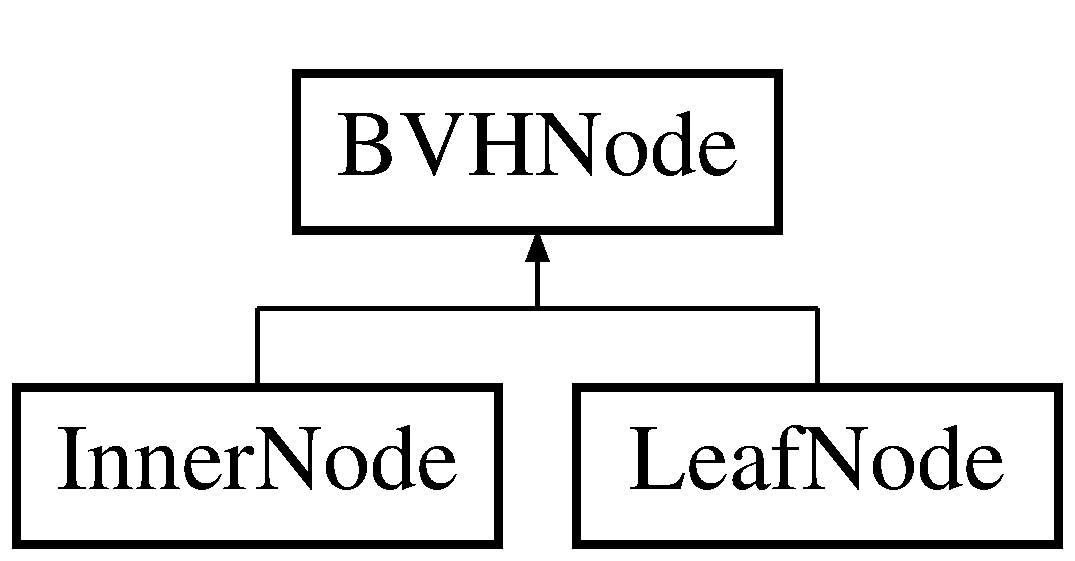
\includegraphics[height=2.000000cm]{classBVHNode}
\end{center}
\end{figure}
\subsection*{Public Member Functions}
\begin{DoxyCompactItemize}
\item 
\hypertarget{classBVHNode_abb536bca7ddda5cd8a21d6246193f3a5}{\hyperlink{classBVHNode_abb536bca7ddda5cd8a21d6246193f3a5}{B\-V\-H\-Node} ()}\label{classBVHNode_abb536bca7ddda5cd8a21d6246193f3a5}

\begin{DoxyCompactList}\small\item\em \hyperlink{classBVHNode}{B\-V\-H\-Node} Empty default ctor,. \end{DoxyCompactList}\item 
\hypertarget{classBVHNode_a77faa5107236f51786cf3e4782d302ac}{virtual \hyperlink{classBVHNode_a77faa5107236f51786cf3e4782d302ac}{$\sim$\-B\-V\-H\-Node} ()}\label{classBVHNode_a77faa5107236f51786cf3e4782d302ac}

\begin{DoxyCompactList}\small\item\em $\sim$\-B\-V\-H\-Node Default virtual dtor \end{DoxyCompactList}\item 
virtual \hyperlink{classBVHNode}{B\-V\-H\-Node} $\ast$ \hyperlink{classBVHNode_acf8b2130dd63bd66e35f130f86c65400}{child\-Node} (const unsigned int \&\-\_\-index) const =0
\begin{DoxyCompactList}\small\item\em child\-Node Virtual method to fetch child nodes of the current node \end{DoxyCompactList}\item 
virtual bool \hyperlink{classBVHNode_a9d6c31fcebf88cc4c128a2b3af1f4cbf}{is\-Leaf} () const =0
\begin{DoxyCompactList}\small\item\em is\-Leaf Whether the current node is a leaf node or not \end{DoxyCompactList}\item 
virtual unsigned int \hyperlink{classBVHNode_ae5ad50686b4c345c98d03f080afc403f}{num\-Child\-Nodes} () const =0
\begin{DoxyCompactList}\small\item\em num\-Child\-Nodes Get the number of child nodes for the current node \end{DoxyCompactList}\item 
virtual unsigned int \hyperlink{classBVHNode_a8a53277e44a407a75e32118ceb4fa425}{num\-Triangles} () const 
\begin{DoxyCompactList}\small\item\em num\-Triangles Get the number of triangles in the current node \end{DoxyCompactList}\item 
\hyperlink{classAABB}{A\-A\-B\-B} \hyperlink{classBVHNode_a6d818bf5517c223d8f7e3fdc9c1f3f37}{get\-Bounds} () const 
\begin{DoxyCompactList}\small\item\em get\-Bounds Get the \hyperlink{classAABB}{A\-A\-B\-B} of the current node \end{DoxyCompactList}\item 
unsigned int \hyperlink{classBVHNode_a5a35ddbaed7b4b4058571f7978938f28}{node\-Count} () const 
\begin{DoxyCompactList}\small\item\em node\-Count Recursively calculate the nodes beneath the current node \end{DoxyCompactList}\item 
float \hyperlink{classBVHNode_a2f6d380d0628de6245d6f364deb92460}{surface\-Area} () const 
\begin{DoxyCompactList}\small\item\em surface\-Area Get the surface area of the nodes \hyperlink{classAABB}{A\-A\-B\-B} \end{DoxyCompactList}\item 
\hypertarget{classBVHNode_a5cdee75dddb4cca21306cbe421772cbd}{void \hyperlink{classBVHNode_a5cdee75dddb4cca21306cbe421772cbd}{clean\-Up} ()}\label{classBVHNode_a5cdee75dddb4cca21306cbe421772cbd}

\begin{DoxyCompactList}\small\item\em clean\-Up Recursively free the allocated memory \end{DoxyCompactList}\end{DoxyCompactItemize}
\subsection*{Protected Attributes}
\begin{DoxyCompactItemize}
\item 
\hypertarget{classBVHNode_af56bc095197988eead3dfdb90c30e96e}{\hyperlink{classAABB}{A\-A\-B\-B} \hyperlink{classBVHNode_af56bc095197988eead3dfdb90c30e96e}{m\-\_\-bounds}}\label{classBVHNode_af56bc095197988eead3dfdb90c30e96e}

\begin{DoxyCompactList}\small\item\em m\-\_\-bounds \hyperlink{classAABB}{A\-A\-B\-B} of the node \end{DoxyCompactList}\end{DoxyCompactItemize}


\subsection{Detailed Description}
The \hyperlink{classBVHNode}{B\-V\-H\-Node} class Abstract base class for the nodes. 

\subsection{Member Function Documentation}
\hypertarget{classBVHNode_acf8b2130dd63bd66e35f130f86c65400}{\index{B\-V\-H\-Node@{B\-V\-H\-Node}!child\-Node@{child\-Node}}
\index{child\-Node@{child\-Node}!BVHNode@{B\-V\-H\-Node}}
\subsubsection[{child\-Node}]{\setlength{\rightskip}{0pt plus 5cm}virtual {\bf B\-V\-H\-Node}$\ast$ B\-V\-H\-Node\-::child\-Node (
\begin{DoxyParamCaption}
\item[{const unsigned int \&}]{\-\_\-index}
\end{DoxyParamCaption}
) const\hspace{0.3cm}{\ttfamily [pure virtual]}}}\label{classBVHNode_acf8b2130dd63bd66e35f130f86c65400}


child\-Node Virtual method to fetch child nodes of the current node 


\begin{DoxyParams}{Parameters}
{\em \-\_\-index} & Index of the child node to get \\
\hline
\end{DoxyParams}
\begin{DoxyReturn}{Returns}
Child node at given index 
\end{DoxyReturn}


Implemented in \hyperlink{classLeafNode_a5c8eac5f86f69e5cae6f41d902550d39}{Leaf\-Node}, and \hyperlink{classInnerNode_af4d76a6913d55b395b30f2ce244b882d}{Inner\-Node}.

\hypertarget{classBVHNode_a6d818bf5517c223d8f7e3fdc9c1f3f37}{\index{B\-V\-H\-Node@{B\-V\-H\-Node}!get\-Bounds@{get\-Bounds}}
\index{get\-Bounds@{get\-Bounds}!BVHNode@{B\-V\-H\-Node}}
\subsubsection[{get\-Bounds}]{\setlength{\rightskip}{0pt plus 5cm}{\bf A\-A\-B\-B} B\-V\-H\-Node\-::get\-Bounds (
\begin{DoxyParamCaption}
{}
\end{DoxyParamCaption}
) const\hspace{0.3cm}{\ttfamily [inline]}}}\label{classBVHNode_a6d818bf5517c223d8f7e3fdc9c1f3f37}


get\-Bounds Get the \hyperlink{classAABB}{A\-A\-B\-B} of the current node 

\begin{DoxyReturn}{Returns}
The aabb 
\end{DoxyReturn}
\hypertarget{classBVHNode_a9d6c31fcebf88cc4c128a2b3af1f4cbf}{\index{B\-V\-H\-Node@{B\-V\-H\-Node}!is\-Leaf@{is\-Leaf}}
\index{is\-Leaf@{is\-Leaf}!BVHNode@{B\-V\-H\-Node}}
\subsubsection[{is\-Leaf}]{\setlength{\rightskip}{0pt plus 5cm}virtual bool B\-V\-H\-Node\-::is\-Leaf (
\begin{DoxyParamCaption}
{}
\end{DoxyParamCaption}
) const\hspace{0.3cm}{\ttfamily [pure virtual]}}}\label{classBVHNode_a9d6c31fcebf88cc4c128a2b3af1f4cbf}


is\-Leaf Whether the current node is a leaf node or not 

\begin{DoxyReturn}{Returns}
True if a leaf node 
\end{DoxyReturn}


Implemented in \hyperlink{classLeafNode_a4971bdbac579dd2d7688aa8706a41ea1}{Leaf\-Node}, and \hyperlink{classInnerNode_a9132770448acf40a331114a350dbe249}{Inner\-Node}.

\hypertarget{classBVHNode_a5a35ddbaed7b4b4058571f7978938f28}{\index{B\-V\-H\-Node@{B\-V\-H\-Node}!node\-Count@{node\-Count}}
\index{node\-Count@{node\-Count}!BVHNode@{B\-V\-H\-Node}}
\subsubsection[{node\-Count}]{\setlength{\rightskip}{0pt plus 5cm}unsigned int B\-V\-H\-Node\-::node\-Count (
\begin{DoxyParamCaption}
{}
\end{DoxyParamCaption}
) const}}\label{classBVHNode_a5a35ddbaed7b4b4058571f7978938f28}


node\-Count Recursively calculate the nodes beneath the current node 

\begin{DoxyReturn}{Returns}
The number of nodes that are children to this node 
\end{DoxyReturn}
\hypertarget{classBVHNode_ae5ad50686b4c345c98d03f080afc403f}{\index{B\-V\-H\-Node@{B\-V\-H\-Node}!num\-Child\-Nodes@{num\-Child\-Nodes}}
\index{num\-Child\-Nodes@{num\-Child\-Nodes}!BVHNode@{B\-V\-H\-Node}}
\subsubsection[{num\-Child\-Nodes}]{\setlength{\rightskip}{0pt plus 5cm}virtual unsigned int B\-V\-H\-Node\-::num\-Child\-Nodes (
\begin{DoxyParamCaption}
{}
\end{DoxyParamCaption}
) const\hspace{0.3cm}{\ttfamily [pure virtual]}}}\label{classBVHNode_ae5ad50686b4c345c98d03f080afc403f}


num\-Child\-Nodes Get the number of child nodes for the current node 

\begin{DoxyReturn}{Returns}
Number of immediate child nodes 
\end{DoxyReturn}


Implemented in \hyperlink{classLeafNode_a897312601f3726f7d20b3d73959c111a}{Leaf\-Node}, and \hyperlink{classInnerNode_a685a9782d88772dfd2ac367025b65848}{Inner\-Node}.

\hypertarget{classBVHNode_a8a53277e44a407a75e32118ceb4fa425}{\index{B\-V\-H\-Node@{B\-V\-H\-Node}!num\-Triangles@{num\-Triangles}}
\index{num\-Triangles@{num\-Triangles}!BVHNode@{B\-V\-H\-Node}}
\subsubsection[{num\-Triangles}]{\setlength{\rightskip}{0pt plus 5cm}virtual unsigned int B\-V\-H\-Node\-::num\-Triangles (
\begin{DoxyParamCaption}
{}
\end{DoxyParamCaption}
) const\hspace{0.3cm}{\ttfamily [inline]}, {\ttfamily [virtual]}}}\label{classBVHNode_a8a53277e44a407a75e32118ceb4fa425}


num\-Triangles Get the number of triangles in the current node 

\begin{DoxyReturn}{Returns}
Number of triangles 
\end{DoxyReturn}


Reimplemented in \hyperlink{classLeafNode_a8c138df453e78a56905e9066fb246f4f}{Leaf\-Node}.

\hypertarget{classBVHNode_a2f6d380d0628de6245d6f364deb92460}{\index{B\-V\-H\-Node@{B\-V\-H\-Node}!surface\-Area@{surface\-Area}}
\index{surface\-Area@{surface\-Area}!BVHNode@{B\-V\-H\-Node}}
\subsubsection[{surface\-Area}]{\setlength{\rightskip}{0pt plus 5cm}float B\-V\-H\-Node\-::surface\-Area (
\begin{DoxyParamCaption}
{}
\end{DoxyParamCaption}
) const}}\label{classBVHNode_a2f6d380d0628de6245d6f364deb92460}


surface\-Area Get the surface area of the nodes \hyperlink{classAABB}{A\-A\-B\-B} 

\begin{DoxyReturn}{Returns}

\end{DoxyReturn}


The documentation for this class was generated from the following files\-:\begin{DoxyCompactItemize}
\item 
include/\hyperlink{BVHNodes_8h}{B\-V\-H\-Nodes.\-h}\item 
src/\hyperlink{BVHNodes_8cpp}{B\-V\-H\-Nodes.\-cpp}\end{DoxyCompactItemize}

\hypertarget{classCamera}{\section{Camera Class Reference}
\label{classCamera}\index{Camera@{Camera}}
}


The \hyperlink{classCamera}{Camera} class Simple camera class that handles movement and rotations, also keeps track whether the camera is dirty e.\-g. if the renderer needs to clear its buffers and start tracing from the beginning.  




{\ttfamily \#include $<$Camera.\-h$>$}

\subsection*{Public Member Functions}
\begin{DoxyCompactItemize}
\item 
\hypertarget{classCamera_a01f94c3543f56ede7af49dc778f19331}{\hyperlink{classCamera_a01f94c3543f56ede7af49dc778f19331}{Camera} ()}\label{classCamera_a01f94c3543f56ede7af49dc778f19331}

\begin{DoxyCompactList}\small\item\em \hyperlink{classCamera}{Camera} Default ctor. \end{DoxyCompactList}\item 
\hypertarget{classCamera_ad1897942d0ccf91052386388a497349f}{\hyperlink{classCamera_ad1897942d0ccf91052386388a497349f}{$\sim$\-Camera} ()}\label{classCamera_ad1897942d0ccf91052386388a497349f}

\begin{DoxyCompactList}\small\item\em $\sim$\-Camera Default dtor \end{DoxyCompactList}\item 
void \hyperlink{classCamera_a132f6e602fdcaabc5d361e6d9392bda2}{pitch} (const float \&\-\_\-angle)
\begin{DoxyCompactList}\small\item\em pitch Add pitch to the camera, triggers the dirty flag \end{DoxyCompactList}\item 
void \hyperlink{classCamera_ae6140b78de760fd0ef9a2c69d6d1018d}{yaw} (const float \&\-\_\-angle)
\begin{DoxyCompactList}\small\item\em yaw Add yaw to the camera, triggers the dirty flag \end{DoxyCompactList}\item 
void \hyperlink{classCamera_af7e91ff00e0259e2917c09d850c50364}{move\-Forward} (const float \&\-\_\-amt)
\begin{DoxyCompactList}\small\item\em move\-Forward Move forward/backward, triggers the dirty flag \end{DoxyCompactList}\item 
void \hyperlink{classCamera_a8d323c4dd7346ff6a46a611108e22e1f}{change\-Fov} (const float \&\-\_\-new\-Fov)
\begin{DoxyCompactList}\small\item\em change\-Fov Change the field of view of the camera, triggers the dirty flag \end{DoxyCompactList}\item 
ngl\-::\-Vec3 \hyperlink{classCamera_a609beb780b3bb52a4b94ec19ca831a9b}{get\-Orig} () const 
\begin{DoxyCompactList}\small\item\em get\-Orig Get the location of the camera \end{DoxyCompactList}\item 
ngl\-::\-Vec3 \hyperlink{classCamera_a2ccd198eae7f90000f53422b760876e0}{get\-Dir} () const 
\begin{DoxyCompactList}\small\item\em get\-Dir Get the direction of the camera \end{DoxyCompactList}\item 
ngl\-::\-Vec3 \hyperlink{classCamera_a375c97c35eb25d7839d85361d1858c3f}{get\-Up} () const 
\begin{DoxyCompactList}\small\item\em get\-Up Get the up vector of the camera \end{DoxyCompactList}\item 
ngl\-::\-Vec3 \hyperlink{classCamera_a19c7285d6919678bc1b11206bfe895fb}{get\-Right} () const 
\begin{DoxyCompactList}\small\item\em get\-Right Get the right vector of the camera \end{DoxyCompactList}\item 
float \hyperlink{classCamera_add207b5f24a14de6bfefb4425f200e15}{get\-Fov\-Scale} () const 
\begin{DoxyCompactList}\small\item\em get\-Fov\-Scale Get the scale used to calculate ray offsets based on the field of view \end{DoxyCompactList}\item 
\hypertarget{classCamera_a2da4f15a13acdc03870b0dca36de7986}{void \hyperlink{classCamera_a2da4f15a13acdc03870b0dca36de7986}{consume} ()}\label{classCamera_a2da4f15a13acdc03870b0dca36de7986}

\begin{DoxyCompactList}\small\item\em consume Update all the vectors and values and reset the dirty flag \end{DoxyCompactList}\item 
bool \hyperlink{classCamera_afd2d3859c75b0f8fa7288a4b70527bf3}{is\-Dirty} () const 
\begin{DoxyCompactList}\small\item\em is\-Dirty Used to check if the camera has updates that need to be consumed \end{DoxyCompactList}\end{DoxyCompactItemize}


\subsection{Detailed Description}
The \hyperlink{classCamera}{Camera} class Simple camera class that handles movement and rotations, also keeps track whether the camera is dirty e.\-g. if the renderer needs to clear its buffers and start tracing from the beginning. 

\subsection{Member Function Documentation}
\hypertarget{classCamera_a8d323c4dd7346ff6a46a611108e22e1f}{\index{Camera@{Camera}!change\-Fov@{change\-Fov}}
\index{change\-Fov@{change\-Fov}!Camera@{Camera}}
\subsubsection[{change\-Fov}]{\setlength{\rightskip}{0pt plus 5cm}void Camera\-::change\-Fov (
\begin{DoxyParamCaption}
\item[{const float \&}]{\-\_\-new\-Fov}
\end{DoxyParamCaption}
)}}\label{classCamera_a8d323c4dd7346ff6a46a611108e22e1f}


change\-Fov Change the field of view of the camera, triggers the dirty flag 


\begin{DoxyParams}{Parameters}
{\em \-\_\-new\-Fov} & New field of view to use \\
\hline
\end{DoxyParams}
\hypertarget{classCamera_a2ccd198eae7f90000f53422b760876e0}{\index{Camera@{Camera}!get\-Dir@{get\-Dir}}
\index{get\-Dir@{get\-Dir}!Camera@{Camera}}
\subsubsection[{get\-Dir}]{\setlength{\rightskip}{0pt plus 5cm}ngl\-::\-Vec3 Camera\-::get\-Dir (
\begin{DoxyParamCaption}
{}
\end{DoxyParamCaption}
) const}}\label{classCamera_a2ccd198eae7f90000f53422b760876e0}


get\-Dir Get the direction of the camera 

\begin{DoxyReturn}{Returns}
The direction, which is the negative forward vector 
\end{DoxyReturn}
\hypertarget{classCamera_add207b5f24a14de6bfefb4425f200e15}{\index{Camera@{Camera}!get\-Fov\-Scale@{get\-Fov\-Scale}}
\index{get\-Fov\-Scale@{get\-Fov\-Scale}!Camera@{Camera}}
\subsubsection[{get\-Fov\-Scale}]{\setlength{\rightskip}{0pt plus 5cm}float Camera\-::get\-Fov\-Scale (
\begin{DoxyParamCaption}
{}
\end{DoxyParamCaption}
) const}}\label{classCamera_add207b5f24a14de6bfefb4425f200e15}


get\-Fov\-Scale Get the scale used to calculate ray offsets based on the field of view 

\begin{DoxyReturn}{Returns}
The field of view scale 
\end{DoxyReturn}
\hypertarget{classCamera_a609beb780b3bb52a4b94ec19ca831a9b}{\index{Camera@{Camera}!get\-Orig@{get\-Orig}}
\index{get\-Orig@{get\-Orig}!Camera@{Camera}}
\subsubsection[{get\-Orig}]{\setlength{\rightskip}{0pt plus 5cm}ngl\-::\-Vec3 Camera\-::get\-Orig (
\begin{DoxyParamCaption}
{}
\end{DoxyParamCaption}
) const}}\label{classCamera_a609beb780b3bb52a4b94ec19ca831a9b}


get\-Orig Get the location of the camera 

\begin{DoxyReturn}{Returns}
Location of the camera in space 
\end{DoxyReturn}
\hypertarget{classCamera_a19c7285d6919678bc1b11206bfe895fb}{\index{Camera@{Camera}!get\-Right@{get\-Right}}
\index{get\-Right@{get\-Right}!Camera@{Camera}}
\subsubsection[{get\-Right}]{\setlength{\rightskip}{0pt plus 5cm}ngl\-::\-Vec3 Camera\-::get\-Right (
\begin{DoxyParamCaption}
{}
\end{DoxyParamCaption}
) const}}\label{classCamera_a19c7285d6919678bc1b11206bfe895fb}


get\-Right Get the right vector of the camera 

\begin{DoxyReturn}{Returns}
Vector perpendicular to the forward and up vectors, facing right 
\end{DoxyReturn}
\hypertarget{classCamera_a375c97c35eb25d7839d85361d1858c3f}{\index{Camera@{Camera}!get\-Up@{get\-Up}}
\index{get\-Up@{get\-Up}!Camera@{Camera}}
\subsubsection[{get\-Up}]{\setlength{\rightskip}{0pt plus 5cm}ngl\-::\-Vec3 Camera\-::get\-Up (
\begin{DoxyParamCaption}
{}
\end{DoxyParamCaption}
) const}}\label{classCamera_a375c97c35eb25d7839d85361d1858c3f}


get\-Up Get the up vector of the camera 

\begin{DoxyReturn}{Returns}
Vector perpendicular to the forward and right vectors, facing upwards 
\end{DoxyReturn}
\hypertarget{classCamera_afd2d3859c75b0f8fa7288a4b70527bf3}{\index{Camera@{Camera}!is\-Dirty@{is\-Dirty}}
\index{is\-Dirty@{is\-Dirty}!Camera@{Camera}}
\subsubsection[{is\-Dirty}]{\setlength{\rightskip}{0pt plus 5cm}bool Camera\-::is\-Dirty (
\begin{DoxyParamCaption}
{}
\end{DoxyParamCaption}
) const}}\label{classCamera_afd2d3859c75b0f8fa7288a4b70527bf3}


is\-Dirty Used to check if the camera has updates that need to be consumed 

\begin{DoxyReturn}{Returns}
Whether the camera is considered dirty 
\end{DoxyReturn}
\hypertarget{classCamera_af7e91ff00e0259e2917c09d850c50364}{\index{Camera@{Camera}!move\-Forward@{move\-Forward}}
\index{move\-Forward@{move\-Forward}!Camera@{Camera}}
\subsubsection[{move\-Forward}]{\setlength{\rightskip}{0pt plus 5cm}void Camera\-::move\-Forward (
\begin{DoxyParamCaption}
\item[{const float \&}]{\-\_\-amt}
\end{DoxyParamCaption}
)}}\label{classCamera_af7e91ff00e0259e2917c09d850c50364}


move\-Forward Move forward/backward, triggers the dirty flag 


\begin{DoxyParams}{Parameters}
{\em \-\_\-amt} & Amount to move \\
\hline
\end{DoxyParams}
\hypertarget{classCamera_a132f6e602fdcaabc5d361e6d9392bda2}{\index{Camera@{Camera}!pitch@{pitch}}
\index{pitch@{pitch}!Camera@{Camera}}
\subsubsection[{pitch}]{\setlength{\rightskip}{0pt plus 5cm}void Camera\-::pitch (
\begin{DoxyParamCaption}
\item[{const float \&}]{\-\_\-angle}
\end{DoxyParamCaption}
)}}\label{classCamera_a132f6e602fdcaabc5d361e6d9392bda2}


pitch Add pitch to the camera, triggers the dirty flag 


\begin{DoxyParams}{Parameters}
{\em \-\_\-angle} & Pitch to add \\
\hline
\end{DoxyParams}
\hypertarget{classCamera_ae6140b78de760fd0ef9a2c69d6d1018d}{\index{Camera@{Camera}!yaw@{yaw}}
\index{yaw@{yaw}!Camera@{Camera}}
\subsubsection[{yaw}]{\setlength{\rightskip}{0pt plus 5cm}void Camera\-::yaw (
\begin{DoxyParamCaption}
\item[{const float \&}]{\-\_\-angle}
\end{DoxyParamCaption}
)}}\label{classCamera_ae6140b78de760fd0ef9a2c69d6d1018d}


yaw Add yaw to the camera, triggers the dirty flag 


\begin{DoxyParams}{Parameters}
{\em \-\_\-angle} & Yaw to add \\
\hline
\end{DoxyParams}


The documentation for this class was generated from the following files\-:\begin{DoxyCompactItemize}
\item 
include/\hyperlink{Camera_8h}{Camera.\-h}\item 
src/\hyperlink{Camera_8cpp}{Camera.\-cpp}\end{DoxyCompactItemize}

\hypertarget{classInnerNode}{\section{Inner\-Node Class Reference}
\label{classInnerNode}\index{Inner\-Node@{Inner\-Node}}
}


The \hyperlink{classInnerNode}{Inner\-Node} class Inner node, e.\-g. a node with children.  




{\ttfamily \#include $<$B\-V\-H\-Nodes.\-h$>$}

Inheritance diagram for Inner\-Node\-:\begin{figure}[H]
\begin{center}
\leavevmode
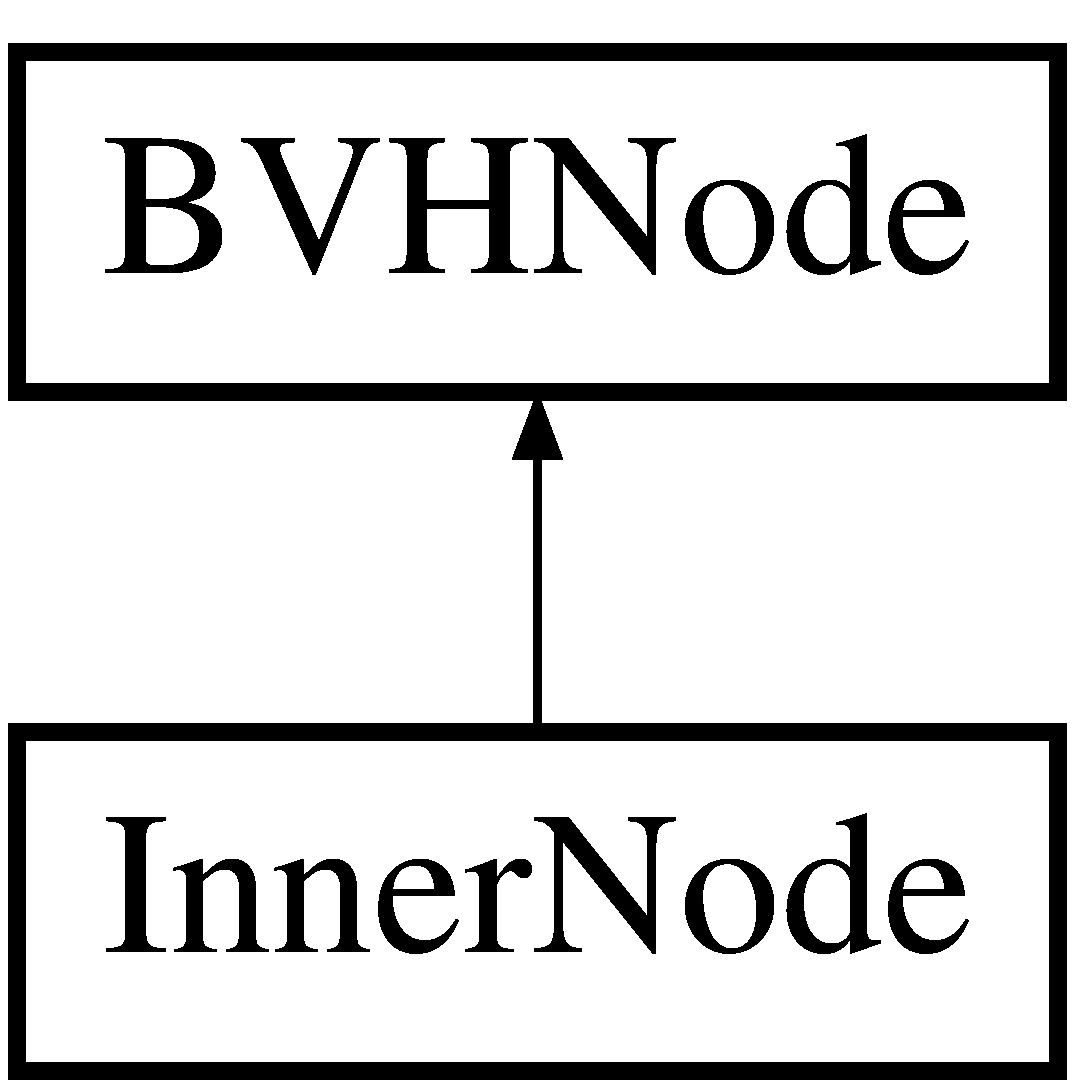
\includegraphics[height=2.000000cm]{classInnerNode}
\end{center}
\end{figure}
\subsection*{Public Member Functions}
\begin{DoxyCompactItemize}
\item 
\hyperlink{classInnerNode_a7ebac6f83b9cc6235b257fdae8e93552}{Inner\-Node} (const \hyperlink{classAABB}{A\-A\-B\-B} \&\-\_\-bounds, \hyperlink{classBVHNode}{B\-V\-H\-Node} $\ast$\-\_\-left\-Child, \hyperlink{classBVHNode}{B\-V\-H\-Node} $\ast$\-\_\-right\-Child)
\begin{DoxyCompactList}\small\item\em \hyperlink{classInnerNode}{Inner\-Node} Default dtor for the inner node, inner node consists of left and right children. \end{DoxyCompactList}\item 
bool \hyperlink{classInnerNode_a9132770448acf40a331114a350dbe249}{is\-Leaf} () const override
\begin{DoxyCompactList}\small\item\em is\-Leaf Inner node is never a leaf but needs to implement this to distinquish the abstract nodes from each other \end{DoxyCompactList}\item 
unsigned int \hyperlink{classInnerNode_a685a9782d88772dfd2ac367025b65848}{num\-Child\-Nodes} () const override
\begin{DoxyCompactList}\small\item\em num\-Child\-Nodes Number of child nodes, an inner node will always have two child nodes; left and right \end{DoxyCompactList}\item 
\hyperlink{classBVHNode}{B\-V\-H\-Node} $\ast$ \hyperlink{classInnerNode_af4d76a6913d55b395b30f2ce244b882d}{child\-Node} (const unsigned int \&\-\_\-index) const override
\begin{DoxyCompactList}\small\item\em child\-Node Get a child node of the current node \end{DoxyCompactList}\end{DoxyCompactItemize}
\subsection*{Additional Inherited Members}


\subsection{Detailed Description}
The \hyperlink{classInnerNode}{Inner\-Node} class Inner node, e.\-g. a node with children. 

\subsection{Constructor \& Destructor Documentation}
\hypertarget{classInnerNode_a7ebac6f83b9cc6235b257fdae8e93552}{\index{Inner\-Node@{Inner\-Node}!Inner\-Node@{Inner\-Node}}
\index{Inner\-Node@{Inner\-Node}!InnerNode@{Inner\-Node}}
\subsubsection[{Inner\-Node}]{\setlength{\rightskip}{0pt plus 5cm}Inner\-Node\-::\-Inner\-Node (
\begin{DoxyParamCaption}
\item[{const {\bf A\-A\-B\-B} \&}]{\-\_\-bounds, }
\item[{{\bf B\-V\-H\-Node} $\ast$}]{\-\_\-left\-Child, }
\item[{{\bf B\-V\-H\-Node} $\ast$}]{\-\_\-right\-Child}
\end{DoxyParamCaption}
)\hspace{0.3cm}{\ttfamily [inline]}}}\label{classInnerNode_a7ebac6f83b9cc6235b257fdae8e93552}


\hyperlink{classInnerNode}{Inner\-Node} Default dtor for the inner node, inner node consists of left and right children. 


\begin{DoxyParams}{Parameters}
{\em \-\_\-bounds} & \hyperlink{classAABB}{A\-A\-B\-B} of the node \\
\hline
{\em \-\_\-left\-Child} & Left child node of the inner node \\
\hline
{\em \-\_\-right\-Child} & Right child node of the inner node \\
\hline
\end{DoxyParams}


\subsection{Member Function Documentation}
\hypertarget{classInnerNode_af4d76a6913d55b395b30f2ce244b882d}{\index{Inner\-Node@{Inner\-Node}!child\-Node@{child\-Node}}
\index{child\-Node@{child\-Node}!InnerNode@{Inner\-Node}}
\subsubsection[{child\-Node}]{\setlength{\rightskip}{0pt plus 5cm}{\bf B\-V\-H\-Node}$\ast$ Inner\-Node\-::child\-Node (
\begin{DoxyParamCaption}
\item[{const unsigned int \&}]{\-\_\-index}
\end{DoxyParamCaption}
) const\hspace{0.3cm}{\ttfamily [inline]}, {\ttfamily [override]}, {\ttfamily [virtual]}}}\label{classInnerNode_af4d76a6913d55b395b30f2ce244b882d}


child\-Node Get a child node of the current node 


\begin{DoxyParams}{Parameters}
{\em \-\_\-index} & Index of the child wanted \\
\hline
\end{DoxyParams}
\begin{DoxyReturn}{Returns}
The child node 
\end{DoxyReturn}


Implements \hyperlink{classBVHNode_acf8b2130dd63bd66e35f130f86c65400}{B\-V\-H\-Node}.

\hypertarget{classInnerNode_a9132770448acf40a331114a350dbe249}{\index{Inner\-Node@{Inner\-Node}!is\-Leaf@{is\-Leaf}}
\index{is\-Leaf@{is\-Leaf}!InnerNode@{Inner\-Node}}
\subsubsection[{is\-Leaf}]{\setlength{\rightskip}{0pt plus 5cm}bool Inner\-Node\-::is\-Leaf (
\begin{DoxyParamCaption}
{}
\end{DoxyParamCaption}
) const\hspace{0.3cm}{\ttfamily [inline]}, {\ttfamily [override]}, {\ttfamily [virtual]}}}\label{classInnerNode_a9132770448acf40a331114a350dbe249}


is\-Leaf Inner node is never a leaf but needs to implement this to distinquish the abstract nodes from each other 

\begin{DoxyReturn}{Returns}
False 
\end{DoxyReturn}


Implements \hyperlink{classBVHNode_a9d6c31fcebf88cc4c128a2b3af1f4cbf}{B\-V\-H\-Node}.

\hypertarget{classInnerNode_a685a9782d88772dfd2ac367025b65848}{\index{Inner\-Node@{Inner\-Node}!num\-Child\-Nodes@{num\-Child\-Nodes}}
\index{num\-Child\-Nodes@{num\-Child\-Nodes}!InnerNode@{Inner\-Node}}
\subsubsection[{num\-Child\-Nodes}]{\setlength{\rightskip}{0pt plus 5cm}unsigned int Inner\-Node\-::num\-Child\-Nodes (
\begin{DoxyParamCaption}
{}
\end{DoxyParamCaption}
) const\hspace{0.3cm}{\ttfamily [inline]}, {\ttfamily [override]}, {\ttfamily [virtual]}}}\label{classInnerNode_a685a9782d88772dfd2ac367025b65848}


num\-Child\-Nodes Number of child nodes, an inner node will always have two child nodes; left and right 

\begin{DoxyReturn}{Returns}
2 
\end{DoxyReturn}


Implements \hyperlink{classBVHNode_ae5ad50686b4c345c98d03f080afc403f}{B\-V\-H\-Node}.



The documentation for this class was generated from the following file\-:\begin{DoxyCompactItemize}
\item 
include/\hyperlink{BVHNodes_8h}{B\-V\-H\-Nodes.\-h}\end{DoxyCompactItemize}

\hypertarget{classLeafNode}{\section{Leaf\-Node Class Reference}
\label{classLeafNode}\index{Leaf\-Node@{Leaf\-Node}}
}


The \hyperlink{classLeafNode}{Leaf\-Node} class Simple leaf node class, stores indices to triangles inside the node.  




{\ttfamily \#include $<$B\-V\-H\-Nodes.\-h$>$}

Inheritance diagram for Leaf\-Node\-:\begin{figure}[H]
\begin{center}
\leavevmode
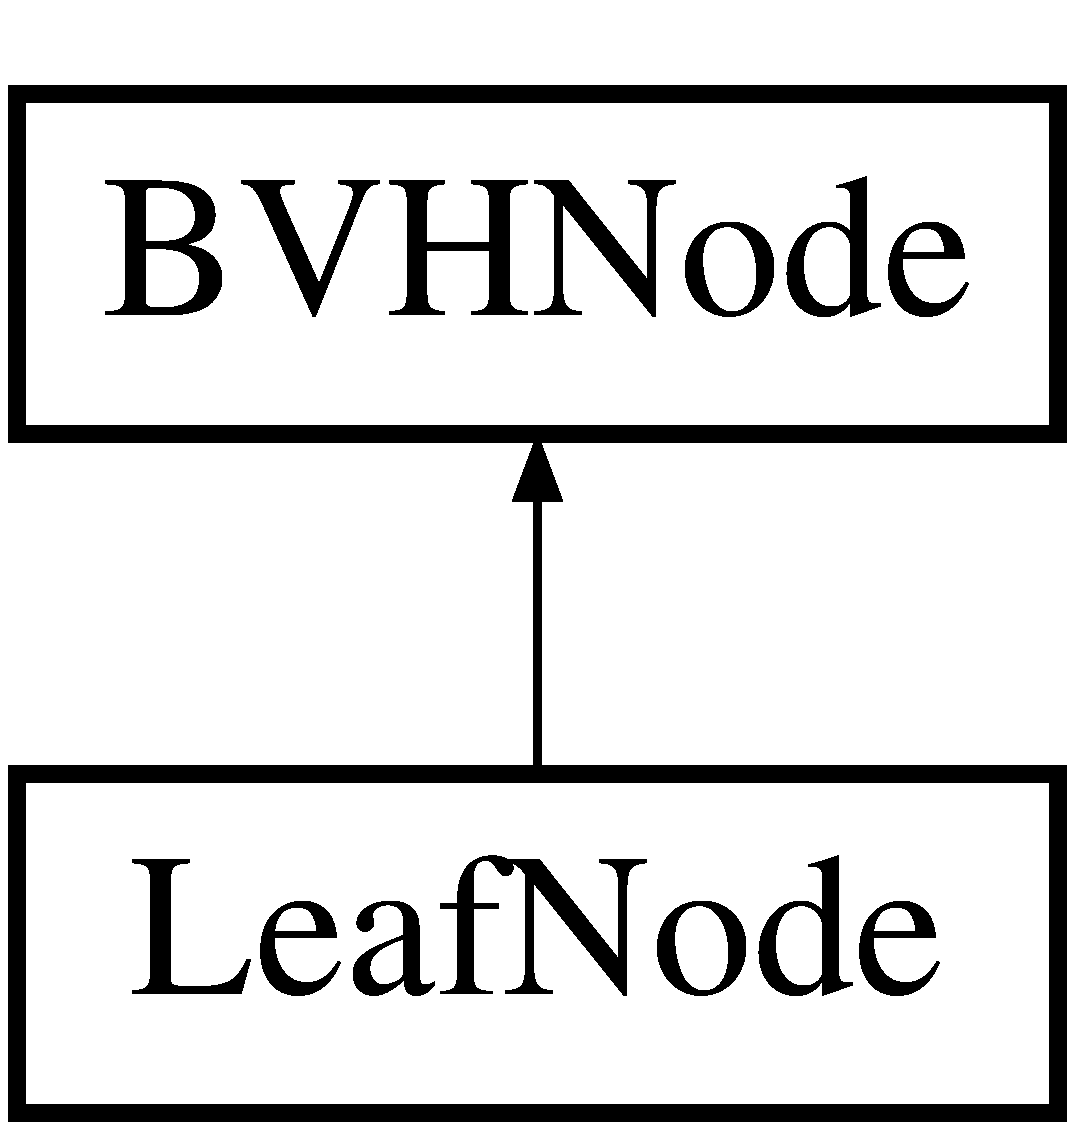
\includegraphics[height=2.000000cm]{classLeafNode}
\end{center}
\end{figure}
\subsection*{Public Member Functions}
\begin{DoxyCompactItemize}
\item 
\hyperlink{classLeafNode_a5d896a0ea632f27c4c62700123a353c5}{Leaf\-Node} (const \hyperlink{classAABB}{A\-A\-B\-B} \&\-\_\-bounds, const unsigned int \&\-\_\-first\-Ind, const unsigned int \&\-\_\-last\-Ind)
\begin{DoxyCompactList}\small\item\em \hyperlink{classLeafNode}{Leaf\-Node} Default ctor for a leaf node. \end{DoxyCompactList}\item 
bool \hyperlink{classLeafNode_a4971bdbac579dd2d7688aa8706a41ea1}{is\-Leaf} () const override
\begin{DoxyCompactList}\small\item\em is\-Leaf Used to distinquish the abstract nodes from each other, will always return true \end{DoxyCompactList}\item 
unsigned int \hyperlink{classLeafNode_a897312601f3726f7d20b3d73959c111a}{num\-Child\-Nodes} () const override
\begin{DoxyCompactList}\small\item\em num\-Child\-Nodes Leaf node has no children but needs to implement the virtual method \end{DoxyCompactList}\item 
\hyperlink{classBVHNode}{B\-V\-H\-Node} $\ast$ \hyperlink{classLeafNode_a5c8eac5f86f69e5cae6f41d902550d39}{child\-Node} (const unsigned int \&\-\_\-index) const override
\begin{DoxyCompactList}\small\item\em child\-Node Leaf node has no children but needs to implement the virtual method \end{DoxyCompactList}\item 
unsigned int \hyperlink{classLeafNode_a8c138df453e78a56905e9066fb246f4f}{num\-Triangles} () const override
\begin{DoxyCompactList}\small\item\em num\-Triangles Get the number of triangles inside the leaf node \end{DoxyCompactList}\item 
unsigned int \hyperlink{classLeafNode_ad354a711fb811f508b682c37ecf2b471}{first\-Index} () const 
\begin{DoxyCompactList}\small\item\em first\-Index Get the first triangle index \end{DoxyCompactList}\item 
unsigned int \hyperlink{classLeafNode_af096e8e428d5f02d02ed16ee182b56d4}{last\-Index} () const 
\begin{DoxyCompactList}\small\item\em last\-Index Get the last triangle index \end{DoxyCompactList}\end{DoxyCompactItemize}
\subsection*{Additional Inherited Members}


\subsection{Detailed Description}
The \hyperlink{classLeafNode}{Leaf\-Node} class Simple leaf node class, stores indices to triangles inside the node. 

\subsection{Constructor \& Destructor Documentation}
\hypertarget{classLeafNode_a5d896a0ea632f27c4c62700123a353c5}{\index{Leaf\-Node@{Leaf\-Node}!Leaf\-Node@{Leaf\-Node}}
\index{Leaf\-Node@{Leaf\-Node}!LeafNode@{Leaf\-Node}}
\subsubsection[{Leaf\-Node}]{\setlength{\rightskip}{0pt plus 5cm}Leaf\-Node\-::\-Leaf\-Node (
\begin{DoxyParamCaption}
\item[{const {\bf A\-A\-B\-B} \&}]{\-\_\-bounds, }
\item[{const unsigned int \&}]{\-\_\-first\-Ind, }
\item[{const unsigned int \&}]{\-\_\-last\-Ind}
\end{DoxyParamCaption}
)\hspace{0.3cm}{\ttfamily [inline]}}}\label{classLeafNode_a5d896a0ea632f27c4c62700123a353c5}


\hyperlink{classLeafNode}{Leaf\-Node} Default ctor for a leaf node. 


\begin{DoxyParams}{Parameters}
{\em \-\_\-bounds} & \hyperlink{classAABB}{A\-A\-B\-B} of the node \\
\hline
{\em \-\_\-first\-Ind} & Index to the first triangle contained by this node \\
\hline
{\em \-\_\-last\-Ind} & Index to the last triangle contained by this node \\
\hline
\end{DoxyParams}


\subsection{Member Function Documentation}
\hypertarget{classLeafNode_a5c8eac5f86f69e5cae6f41d902550d39}{\index{Leaf\-Node@{Leaf\-Node}!child\-Node@{child\-Node}}
\index{child\-Node@{child\-Node}!LeafNode@{Leaf\-Node}}
\subsubsection[{child\-Node}]{\setlength{\rightskip}{0pt plus 5cm}{\bf B\-V\-H\-Node}$\ast$ Leaf\-Node\-::child\-Node (
\begin{DoxyParamCaption}
\item[{const unsigned int \&}]{\-\_\-index}
\end{DoxyParamCaption}
) const\hspace{0.3cm}{\ttfamily [inline]}, {\ttfamily [override]}, {\ttfamily [virtual]}}}\label{classLeafNode_a5c8eac5f86f69e5cae6f41d902550d39}


child\-Node Leaf node has no children but needs to implement the virtual method 


\begin{DoxyParams}{Parameters}
{\em \-\_\-index} & Index to the child \\
\hline
\end{DoxyParams}
\begin{DoxyReturn}{Returns}
nullptr as there are no children 
\end{DoxyReturn}


Implements \hyperlink{classBVHNode_acf8b2130dd63bd66e35f130f86c65400}{B\-V\-H\-Node}.

\hypertarget{classLeafNode_ad354a711fb811f508b682c37ecf2b471}{\index{Leaf\-Node@{Leaf\-Node}!first\-Index@{first\-Index}}
\index{first\-Index@{first\-Index}!LeafNode@{Leaf\-Node}}
\subsubsection[{first\-Index}]{\setlength{\rightskip}{0pt plus 5cm}unsigned int Leaf\-Node\-::first\-Index (
\begin{DoxyParamCaption}
{}
\end{DoxyParamCaption}
) const\hspace{0.3cm}{\ttfamily [inline]}}}\label{classLeafNode_ad354a711fb811f508b682c37ecf2b471}


first\-Index Get the first triangle index 

\begin{DoxyReturn}{Returns}
Index to the first triangle 
\end{DoxyReturn}
\hypertarget{classLeafNode_a4971bdbac579dd2d7688aa8706a41ea1}{\index{Leaf\-Node@{Leaf\-Node}!is\-Leaf@{is\-Leaf}}
\index{is\-Leaf@{is\-Leaf}!LeafNode@{Leaf\-Node}}
\subsubsection[{is\-Leaf}]{\setlength{\rightskip}{0pt plus 5cm}bool Leaf\-Node\-::is\-Leaf (
\begin{DoxyParamCaption}
{}
\end{DoxyParamCaption}
) const\hspace{0.3cm}{\ttfamily [inline]}, {\ttfamily [override]}, {\ttfamily [virtual]}}}\label{classLeafNode_a4971bdbac579dd2d7688aa8706a41ea1}


is\-Leaf Used to distinquish the abstract nodes from each other, will always return true 

\begin{DoxyReturn}{Returns}
True 
\end{DoxyReturn}


Implements \hyperlink{classBVHNode_a9d6c31fcebf88cc4c128a2b3af1f4cbf}{B\-V\-H\-Node}.

\hypertarget{classLeafNode_af096e8e428d5f02d02ed16ee182b56d4}{\index{Leaf\-Node@{Leaf\-Node}!last\-Index@{last\-Index}}
\index{last\-Index@{last\-Index}!LeafNode@{Leaf\-Node}}
\subsubsection[{last\-Index}]{\setlength{\rightskip}{0pt plus 5cm}unsigned int Leaf\-Node\-::last\-Index (
\begin{DoxyParamCaption}
{}
\end{DoxyParamCaption}
) const\hspace{0.3cm}{\ttfamily [inline]}}}\label{classLeafNode_af096e8e428d5f02d02ed16ee182b56d4}


last\-Index Get the last triangle index 

\begin{DoxyReturn}{Returns}
Index to the last triangle 
\end{DoxyReturn}
\hypertarget{classLeafNode_a897312601f3726f7d20b3d73959c111a}{\index{Leaf\-Node@{Leaf\-Node}!num\-Child\-Nodes@{num\-Child\-Nodes}}
\index{num\-Child\-Nodes@{num\-Child\-Nodes}!LeafNode@{Leaf\-Node}}
\subsubsection[{num\-Child\-Nodes}]{\setlength{\rightskip}{0pt plus 5cm}unsigned int Leaf\-Node\-::num\-Child\-Nodes (
\begin{DoxyParamCaption}
{}
\end{DoxyParamCaption}
) const\hspace{0.3cm}{\ttfamily [inline]}, {\ttfamily [override]}, {\ttfamily [virtual]}}}\label{classLeafNode_a897312601f3726f7d20b3d73959c111a}


num\-Child\-Nodes Leaf node has no children but needs to implement the virtual method 

\begin{DoxyReturn}{Returns}
0 
\end{DoxyReturn}


Implements \hyperlink{classBVHNode_ae5ad50686b4c345c98d03f080afc403f}{B\-V\-H\-Node}.

\hypertarget{classLeafNode_a8c138df453e78a56905e9066fb246f4f}{\index{Leaf\-Node@{Leaf\-Node}!num\-Triangles@{num\-Triangles}}
\index{num\-Triangles@{num\-Triangles}!LeafNode@{Leaf\-Node}}
\subsubsection[{num\-Triangles}]{\setlength{\rightskip}{0pt plus 5cm}unsigned int Leaf\-Node\-::num\-Triangles (
\begin{DoxyParamCaption}
{}
\end{DoxyParamCaption}
) const\hspace{0.3cm}{\ttfamily [inline]}, {\ttfamily [override]}, {\ttfamily [virtual]}}}\label{classLeafNode_a8c138df453e78a56905e9066fb246f4f}


num\-Triangles Get the number of triangles inside the leaf node 

\begin{DoxyReturn}{Returns}
The number of triangles contained by the node, e.\-g. last index -\/ first index 
\end{DoxyReturn}


Reimplemented from \hyperlink{classBVHNode_a8a53277e44a407a75e32118ceb4fa425}{B\-V\-H\-Node}.



The documentation for this class was generated from the following file\-:\begin{DoxyCompactItemize}
\item 
include/\hyperlink{BVHNodes_8h}{B\-V\-H\-Nodes.\-h}\end{DoxyCompactItemize}

\hypertarget{classUi_1_1MainWindow}{\section{Ui\-:\-:Main\-Window Class Reference}
\label{classUi_1_1MainWindow}\index{Ui\-::\-Main\-Window@{Ui\-::\-Main\-Window}}
}
Inheritance diagram for Ui\-:\-:Main\-Window\-:\begin{figure}[H]
\begin{center}
\leavevmode
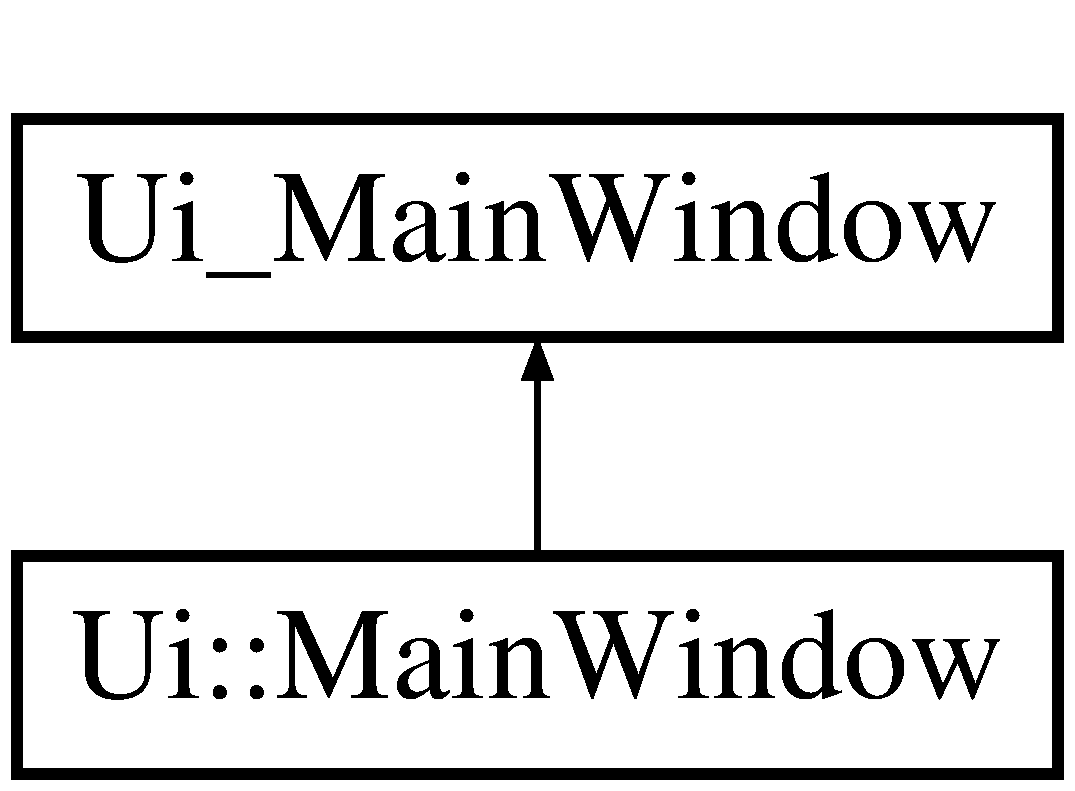
\includegraphics[height=2.000000cm]{classUi_1_1MainWindow}
\end{center}
\end{figure}
\subsection*{Additional Inherited Members}


The documentation for this class was generated from the following file\-:\begin{DoxyCompactItemize}
\item 
ui\-\_\-mainwindow.\-h\end{DoxyCompactItemize}

\hypertarget{classMainWindow}{\section{Main\-Window Class Reference}
\label{classMainWindow}\index{Main\-Window@{Main\-Window}}
}


The \hyperlink{classMainWindow}{Main\-Window} class.  




{\ttfamily \#include $<$mainwindow.\-h$>$}

Inheritance diagram for Main\-Window\-:\begin{figure}[H]
\begin{center}
\leavevmode
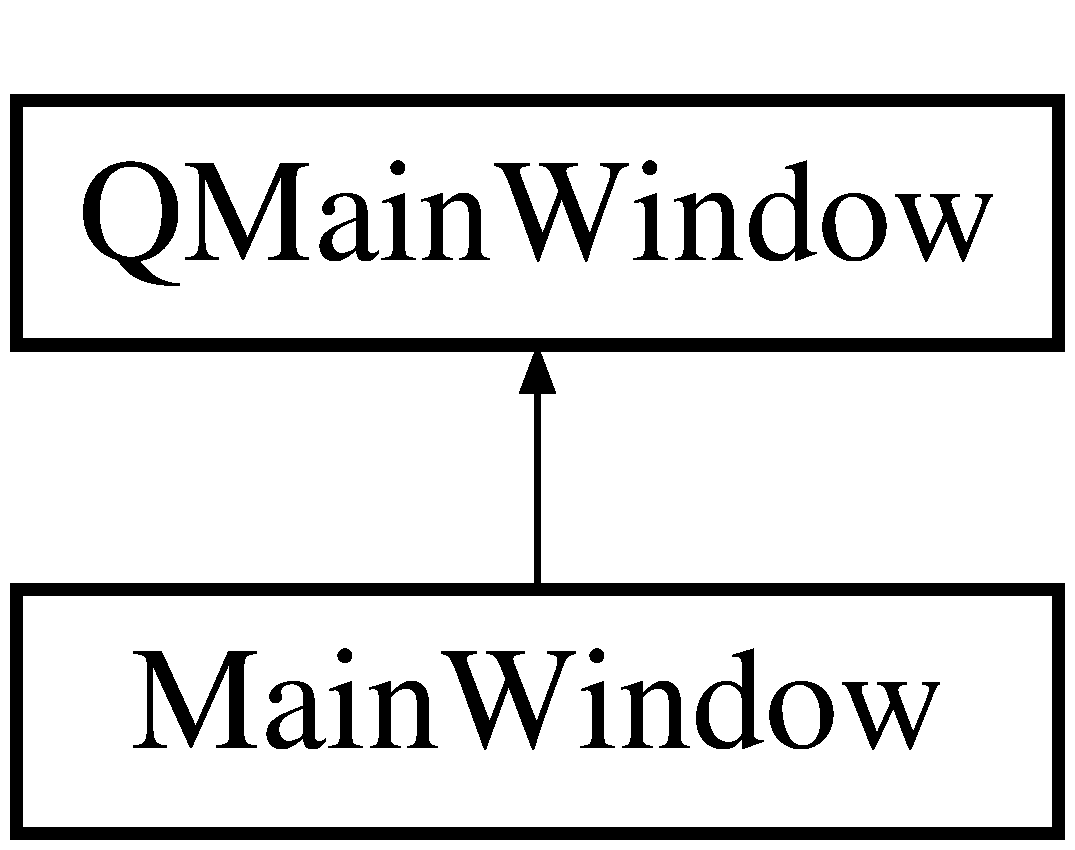
\includegraphics[height=2.000000cm]{classMainWindow}
\end{center}
\end{figure}
\subsection*{Public Slots}
\begin{DoxyCompactItemize}
\item 
void \hyperlink{classMainWindow_a8e0e73b8bba2c32a5f1a3c6a0ae5089d}{update\-U\-I\-Scene\-Tree} (const Q\-String \&\-\_\-mesh)
\begin{DoxyCompactList}\small\item\em update\-U\-I\-Scene\-Tree Adds new meshes to the scene tree in the U\-I \end{DoxyCompactList}\item 
void \hyperlink{classMainWindow_acf4fa9e3d00f6b0d368d6cf7868b618a}{update\-U\-I\-Texture} (const Q\-String \&\-\_\-texture, const unsigned int \&\-\_\-type)
\begin{DoxyCompactList}\small\item\em update\-U\-I\-Texture Updates the path of a loaded texture to the U\-I \end{DoxyCompactList}\item 
void \hyperlink{classMainWindow_a94c97346b7f1e4f0d35844e9d193a79c}{update\-U\-I\-B\-R\-D\-F} (const Q\-String \&\-\_\-brdf)
\begin{DoxyCompactList}\small\item\em update\-U\-I\-B\-R\-D\-F Updates the path of a loaded B\-R\-D\-F to the U\-I \end{DoxyCompactList}\item 
void \hyperlink{classMainWindow_ada92e077013a39ba4fffb39385b8f8d3}{update\-U\-I\-H\-D\-R\-I} (const Q\-String \&\-\_\-hdri)
\begin{DoxyCompactList}\small\item\em update\-U\-I\-H\-D\-R\-I Updates the path of a loaded H\-D\-R\-I to the U\-I \end{DoxyCompactList}\item 
void \hyperlink{classMainWindow_a3e635401d6f115c89799ccb4be12f4f2}{update\-U\-I\-F\-O\-V} (const int \&\-\_\-new\-Fov)
\begin{DoxyCompactList}\small\item\em update\-U\-I\-F\-O\-V Updates the Field of View display in the U\-I \end{DoxyCompactList}\item 
void \hyperlink{classMainWindow_aab6c5078d2405b7938278b53fc8b9c14}{update\-U\-I\-Fresnel\-Coef} (const int \&\-\_\-new\-Val)
\begin{DoxyCompactList}\small\item\em update\-U\-I\-Fresnel\-Coef Updates the fresnel coefficient display in the U\-I \end{DoxyCompactList}\item 
void \hyperlink{classMainWindow_aeee147386c4fe45b4982baa47bd1279f}{update\-U\-I\-Fresnel\-Pow} (const int \&\-\_\-new\-Val)
\begin{DoxyCompactList}\small\item\em update\-U\-I\-Fresnel\-Pow Updates the fresnel power display in the U\-I \end{DoxyCompactList}\item 
void \hyperlink{classMainWindow_a5d1e3243d8388757e82037391ffd677b}{update\-U\-I\-F\-X\-A\-A\-Softness} (const int \&\-\_\-new\-Val)
\begin{DoxyCompactList}\small\item\em update\-U\-I\-F\-X\-A\-A\-Softness Updates the F\-X\-A\-A softness/sharpness display in the U\-I \end{DoxyCompactList}\item 
void \hyperlink{classMainWindow_a6483ad1b0e680d1a1627295f76ce6f4a}{update\-U\-I\-F\-X\-A\-A\-Edge\-Threshold} (const int \&\-\_\-new\-Val)
\begin{DoxyCompactList}\small\item\em update\-U\-I\-F\-X\-A\-A\-Edge\-Threshold Updates the F\-X\-A\-A edge threshold display in the U\-I \end{DoxyCompactList}\item 
void \hyperlink{classMainWindow_ac5f09fce95033810b6fcb286547ad306}{update\-U\-I\-F\-X\-A\-A\-Subpix\-Quality} (const int \&\-\_\-new\-Val)
\begin{DoxyCompactList}\small\item\em update\-U\-I\-F\-X\-A\-A\-Subpix\-Quality Updates the F\-X\-A\-A subpixel quality display in the U\-I \end{DoxyCompactList}\end{DoxyCompactItemize}
\subsection*{Public Member Functions}
\begin{DoxyCompactItemize}
\item 
\hyperlink{classMainWindow_a93cfdcac35db98baf6a7d2c2738a2006}{Main\-Window} (Q\-Widget $\ast$\-\_\-parent=0)
\begin{DoxyCompactList}\small\item\em \hyperlink{classMainWindow}{Main\-Window} Default ctor, allocates the scene and connects used signals and slots. \end{DoxyCompactList}\item 
\hypertarget{classMainWindow_ae98d00a93bc118200eeef9f9bba1dba7}{\hyperlink{classMainWindow_ae98d00a93bc118200eeef9f9bba1dba7}{$\sim$\-Main\-Window} ()}\label{classMainWindow_ae98d00a93bc118200eeef9f9bba1dba7}

\begin{DoxyCompactList}\small\item\em Default dtor, handles basic clean up. \end{DoxyCompactList}\item 
void \hyperlink{classMainWindow_a96e417ae020ed57805409b2481a3d707}{key\-Press\-Event} (Q\-Key\-Event $\ast$\-\_\-event) override
\begin{DoxyCompactList}\small\item\em key\-Press\-Event Handles simple keypress events, \end{DoxyCompactList}\end{DoxyCompactItemize}


\subsection{Detailed Description}
The \hyperlink{classMainWindow}{Main\-Window} class. 

\subsection{Constructor \& Destructor Documentation}
\hypertarget{classMainWindow_a93cfdcac35db98baf6a7d2c2738a2006}{\index{Main\-Window@{Main\-Window}!Main\-Window@{Main\-Window}}
\index{Main\-Window@{Main\-Window}!MainWindow@{Main\-Window}}
\subsubsection[{Main\-Window}]{\setlength{\rightskip}{0pt plus 5cm}Main\-Window\-::\-Main\-Window (
\begin{DoxyParamCaption}
\item[{Q\-Widget $\ast$}]{\-\_\-parent = {\ttfamily 0}}
\end{DoxyParamCaption}
)\hspace{0.3cm}{\ttfamily [explicit]}}}\label{classMainWindow_a93cfdcac35db98baf6a7d2c2738a2006}


\hyperlink{classMainWindow}{Main\-Window} Default ctor, allocates the scene and connects used signals and slots. 


\begin{DoxyParams}{Parameters}
{\em \-\_\-parent} & Parent widget, passed on to the Q\-Main\-Window \\
\hline
\end{DoxyParams}
S\-I\-G\-N\-A\-L-\/\-S\-L\-O\-T connections 

\subsection{Member Function Documentation}
\hypertarget{classMainWindow_a96e417ae020ed57805409b2481a3d707}{\index{Main\-Window@{Main\-Window}!key\-Press\-Event@{key\-Press\-Event}}
\index{key\-Press\-Event@{key\-Press\-Event}!MainWindow@{Main\-Window}}
\subsubsection[{key\-Press\-Event}]{\setlength{\rightskip}{0pt plus 5cm}void Main\-Window\-::key\-Press\-Event (
\begin{DoxyParamCaption}
\item[{Q\-Key\-Event $\ast$}]{\-\_\-event}
\end{DoxyParamCaption}
)\hspace{0.3cm}{\ttfamily [override]}}}\label{classMainWindow_a96e417ae020ed57805409b2481a3d707}


key\-Press\-Event Handles simple keypress events, 


\begin{DoxyParams}{Parameters}
{\em \-\_\-event} & Event containing the keypress data \\
\hline
\end{DoxyParams}
\hypertarget{classMainWindow_a94c97346b7f1e4f0d35844e9d193a79c}{\index{Main\-Window@{Main\-Window}!update\-U\-I\-B\-R\-D\-F@{update\-U\-I\-B\-R\-D\-F}}
\index{update\-U\-I\-B\-R\-D\-F@{update\-U\-I\-B\-R\-D\-F}!MainWindow@{Main\-Window}}
\subsubsection[{update\-U\-I\-B\-R\-D\-F}]{\setlength{\rightskip}{0pt plus 5cm}void Main\-Window\-::update\-U\-I\-B\-R\-D\-F (
\begin{DoxyParamCaption}
\item[{const Q\-String \&}]{\-\_\-brdf}
\end{DoxyParamCaption}
)\hspace{0.3cm}{\ttfamily [slot]}}}\label{classMainWindow_a94c97346b7f1e4f0d35844e9d193a79c}


update\-U\-I\-B\-R\-D\-F Updates the path of a loaded B\-R\-D\-F to the U\-I 


\begin{DoxyParams}{Parameters}
{\em \-\_\-brdf} & Path to the loaded B\-R\-D\-F binary \\
\hline
\end{DoxyParams}
\hypertarget{classMainWindow_a3e635401d6f115c89799ccb4be12f4f2}{\index{Main\-Window@{Main\-Window}!update\-U\-I\-F\-O\-V@{update\-U\-I\-F\-O\-V}}
\index{update\-U\-I\-F\-O\-V@{update\-U\-I\-F\-O\-V}!MainWindow@{Main\-Window}}
\subsubsection[{update\-U\-I\-F\-O\-V}]{\setlength{\rightskip}{0pt plus 5cm}void Main\-Window\-::update\-U\-I\-F\-O\-V (
\begin{DoxyParamCaption}
\item[{const int \&}]{\-\_\-new\-Fov}
\end{DoxyParamCaption}
)\hspace{0.3cm}{\ttfamily [slot]}}}\label{classMainWindow_a3e635401d6f115c89799ccb4be12f4f2}


update\-U\-I\-F\-O\-V Updates the Field of View display in the U\-I 


\begin{DoxyParams}{Parameters}
{\em \-\_\-new\-Fov} & Updated F\-O\-V value \\
\hline
\end{DoxyParams}
\hypertarget{classMainWindow_aab6c5078d2405b7938278b53fc8b9c14}{\index{Main\-Window@{Main\-Window}!update\-U\-I\-Fresnel\-Coef@{update\-U\-I\-Fresnel\-Coef}}
\index{update\-U\-I\-Fresnel\-Coef@{update\-U\-I\-Fresnel\-Coef}!MainWindow@{Main\-Window}}
\subsubsection[{update\-U\-I\-Fresnel\-Coef}]{\setlength{\rightskip}{0pt plus 5cm}void Main\-Window\-::update\-U\-I\-Fresnel\-Coef (
\begin{DoxyParamCaption}
\item[{const int \&}]{\-\_\-new\-Val}
\end{DoxyParamCaption}
)\hspace{0.3cm}{\ttfamily [slot]}}}\label{classMainWindow_aab6c5078d2405b7938278b53fc8b9c14}


update\-U\-I\-Fresnel\-Coef Updates the fresnel coefficient display in the U\-I 


\begin{DoxyParams}{Parameters}
{\em \-\_\-new\-Val} & Updated fresnel coefficient \\
\hline
\end{DoxyParams}
\hypertarget{classMainWindow_aeee147386c4fe45b4982baa47bd1279f}{\index{Main\-Window@{Main\-Window}!update\-U\-I\-Fresnel\-Pow@{update\-U\-I\-Fresnel\-Pow}}
\index{update\-U\-I\-Fresnel\-Pow@{update\-U\-I\-Fresnel\-Pow}!MainWindow@{Main\-Window}}
\subsubsection[{update\-U\-I\-Fresnel\-Pow}]{\setlength{\rightskip}{0pt plus 5cm}void Main\-Window\-::update\-U\-I\-Fresnel\-Pow (
\begin{DoxyParamCaption}
\item[{const int \&}]{\-\_\-new\-Val}
\end{DoxyParamCaption}
)\hspace{0.3cm}{\ttfamily [slot]}}}\label{classMainWindow_aeee147386c4fe45b4982baa47bd1279f}


update\-U\-I\-Fresnel\-Pow Updates the fresnel power display in the U\-I 


\begin{DoxyParams}{Parameters}
{\em \-\_\-new\-Val} & Updated fresnel power \\
\hline
\end{DoxyParams}
\hypertarget{classMainWindow_a6483ad1b0e680d1a1627295f76ce6f4a}{\index{Main\-Window@{Main\-Window}!update\-U\-I\-F\-X\-A\-A\-Edge\-Threshold@{update\-U\-I\-F\-X\-A\-A\-Edge\-Threshold}}
\index{update\-U\-I\-F\-X\-A\-A\-Edge\-Threshold@{update\-U\-I\-F\-X\-A\-A\-Edge\-Threshold}!MainWindow@{Main\-Window}}
\subsubsection[{update\-U\-I\-F\-X\-A\-A\-Edge\-Threshold}]{\setlength{\rightskip}{0pt plus 5cm}void Main\-Window\-::update\-U\-I\-F\-X\-A\-A\-Edge\-Threshold (
\begin{DoxyParamCaption}
\item[{const int \&}]{\-\_\-new\-Val}
\end{DoxyParamCaption}
)\hspace{0.3cm}{\ttfamily [slot]}}}\label{classMainWindow_a6483ad1b0e680d1a1627295f76ce6f4a}


update\-U\-I\-F\-X\-A\-A\-Edge\-Threshold Updates the F\-X\-A\-A edge threshold display in the U\-I 


\begin{DoxyParams}{Parameters}
{\em \-\_\-new\-Val} & New edge threshold \\
\hline
\end{DoxyParams}
\hypertarget{classMainWindow_a5d1e3243d8388757e82037391ffd677b}{\index{Main\-Window@{Main\-Window}!update\-U\-I\-F\-X\-A\-A\-Softness@{update\-U\-I\-F\-X\-A\-A\-Softness}}
\index{update\-U\-I\-F\-X\-A\-A\-Softness@{update\-U\-I\-F\-X\-A\-A\-Softness}!MainWindow@{Main\-Window}}
\subsubsection[{update\-U\-I\-F\-X\-A\-A\-Softness}]{\setlength{\rightskip}{0pt plus 5cm}void Main\-Window\-::update\-U\-I\-F\-X\-A\-A\-Softness (
\begin{DoxyParamCaption}
\item[{const int \&}]{\-\_\-new\-Val}
\end{DoxyParamCaption}
)\hspace{0.3cm}{\ttfamily [slot]}}}\label{classMainWindow_a5d1e3243d8388757e82037391ffd677b}


update\-U\-I\-F\-X\-A\-A\-Softness Updates the F\-X\-A\-A softness/sharpness display in the U\-I 


\begin{DoxyParams}{Parameters}
{\em \-\_\-new\-Val} & Updated F\-X\-A\-A sharpness value \\
\hline
\end{DoxyParams}
\hypertarget{classMainWindow_ac5f09fce95033810b6fcb286547ad306}{\index{Main\-Window@{Main\-Window}!update\-U\-I\-F\-X\-A\-A\-Subpix\-Quality@{update\-U\-I\-F\-X\-A\-A\-Subpix\-Quality}}
\index{update\-U\-I\-F\-X\-A\-A\-Subpix\-Quality@{update\-U\-I\-F\-X\-A\-A\-Subpix\-Quality}!MainWindow@{Main\-Window}}
\subsubsection[{update\-U\-I\-F\-X\-A\-A\-Subpix\-Quality}]{\setlength{\rightskip}{0pt plus 5cm}void Main\-Window\-::update\-U\-I\-F\-X\-A\-A\-Subpix\-Quality (
\begin{DoxyParamCaption}
\item[{const int \&}]{\-\_\-new\-Val}
\end{DoxyParamCaption}
)\hspace{0.3cm}{\ttfamily [slot]}}}\label{classMainWindow_ac5f09fce95033810b6fcb286547ad306}


update\-U\-I\-F\-X\-A\-A\-Subpix\-Quality Updates the F\-X\-A\-A subpixel quality display in the U\-I 


\begin{DoxyParams}{Parameters}
{\em \-\_\-new\-Val} & Updated subpixel quality value \\
\hline
\end{DoxyParams}
\hypertarget{classMainWindow_ada92e077013a39ba4fffb39385b8f8d3}{\index{Main\-Window@{Main\-Window}!update\-U\-I\-H\-D\-R\-I@{update\-U\-I\-H\-D\-R\-I}}
\index{update\-U\-I\-H\-D\-R\-I@{update\-U\-I\-H\-D\-R\-I}!MainWindow@{Main\-Window}}
\subsubsection[{update\-U\-I\-H\-D\-R\-I}]{\setlength{\rightskip}{0pt plus 5cm}void Main\-Window\-::update\-U\-I\-H\-D\-R\-I (
\begin{DoxyParamCaption}
\item[{const Q\-String \&}]{\-\_\-hdri}
\end{DoxyParamCaption}
)\hspace{0.3cm}{\ttfamily [slot]}}}\label{classMainWindow_ada92e077013a39ba4fffb39385b8f8d3}


update\-U\-I\-H\-D\-R\-I Updates the path of a loaded H\-D\-R\-I to the U\-I 


\begin{DoxyParams}{Parameters}
{\em \-\_\-hdri} & Path to the loaded H\-D\-R\-I map \\
\hline
\end{DoxyParams}
\hypertarget{classMainWindow_a8e0e73b8bba2c32a5f1a3c6a0ae5089d}{\index{Main\-Window@{Main\-Window}!update\-U\-I\-Scene\-Tree@{update\-U\-I\-Scene\-Tree}}
\index{update\-U\-I\-Scene\-Tree@{update\-U\-I\-Scene\-Tree}!MainWindow@{Main\-Window}}
\subsubsection[{update\-U\-I\-Scene\-Tree}]{\setlength{\rightskip}{0pt plus 5cm}void Main\-Window\-::update\-U\-I\-Scene\-Tree (
\begin{DoxyParamCaption}
\item[{const Q\-String \&}]{\-\_\-mesh}
\end{DoxyParamCaption}
)\hspace{0.3cm}{\ttfamily [slot]}}}\label{classMainWindow_a8e0e73b8bba2c32a5f1a3c6a0ae5089d}


update\-U\-I\-Scene\-Tree Adds new meshes to the scene tree in the U\-I 


\begin{DoxyParams}{Parameters}
{\em \-\_\-mesh} & Name of the mesh \\
\hline
\end{DoxyParams}
\hypertarget{classMainWindow_acf4fa9e3d00f6b0d368d6cf7868b618a}{\index{Main\-Window@{Main\-Window}!update\-U\-I\-Texture@{update\-U\-I\-Texture}}
\index{update\-U\-I\-Texture@{update\-U\-I\-Texture}!MainWindow@{Main\-Window}}
\subsubsection[{update\-U\-I\-Texture}]{\setlength{\rightskip}{0pt plus 5cm}void Main\-Window\-::update\-U\-I\-Texture (
\begin{DoxyParamCaption}
\item[{const Q\-String \&}]{\-\_\-texture, }
\item[{const unsigned int \&}]{\-\_\-type}
\end{DoxyParamCaption}
)\hspace{0.3cm}{\ttfamily [slot]}}}\label{classMainWindow_acf4fa9e3d00f6b0d368d6cf7868b618a}


update\-U\-I\-Texture Updates the path of a loaded texture to the U\-I 


\begin{DoxyParams}{Parameters}
{\em \-\_\-texture} & Path to the loaded texture \\
\hline
{\em \-\_\-type} & Texture type, 0 = Diffuse, 1 = Normal, 2 = Specular \\
\hline
\end{DoxyParams}


The documentation for this class was generated from the following files\-:\begin{DoxyCompactItemize}
\item 
include/mainwindow.\-h\item 
src/mainwindow.\-cpp\end{DoxyCompactItemize}

\hypertarget{structmat4}{\section{mat4 Struct Reference}
\label{structmat4}\index{mat4@{mat4}}
}


Simple \hyperlink{structmat4}{mat4} struct used for normal map calculations.  


\subsection*{Public Member Functions}
\begin{DoxyCompactItemize}
\item 
\-\_\-\-\_\-device\-\_\-\-\_\- \hyperlink{structmat4_a5d51b0d9907ab69afff96ddc8a12aaba}{mat4} (const float4 \-\_\-a=make\-\_\-float4(1.f, 0.f, 0.f, 0.f), const float4 \-\_\-b=make\-\_\-float4(0.f, 1.f, 0.f, 0.f), const float4 \-\_\-c=make\-\_\-float4(0.f, 0.f, 1.f, 0.f), const float4 \-\_\-d=make\-\_\-float4(0.f, 0.f, 0.f, 1.f))
\begin{DoxyCompactList}\small\item\em \hyperlink{structmat4}{mat4} Default ctor for the matrix \end{DoxyCompactList}\end{DoxyCompactItemize}
\subsection*{Public Attributes}
\begin{DoxyCompactItemize}
\item 
\hypertarget{structmat4_a8164befea75e083db99208f2a1efc2d1}{float4 \hyperlink{structmat4_a8164befea75e083db99208f2a1efc2d1}{m\-\_\-0}}\label{structmat4_a8164befea75e083db99208f2a1efc2d1}

\begin{DoxyCompactList}\small\item\em m\-\_\-0 First row of the matrix \end{DoxyCompactList}\item 
\hypertarget{structmat4_ac4662700e6b5e12aca44fdc20eb9f1f9}{float4 \hyperlink{structmat4_ac4662700e6b5e12aca44fdc20eb9f1f9}{m\-\_\-1}}\label{structmat4_ac4662700e6b5e12aca44fdc20eb9f1f9}

\begin{DoxyCompactList}\small\item\em m\-\_\-1 Second row of the matrix \end{DoxyCompactList}\item 
\hypertarget{structmat4_abcc223150819c1d631d1ae43d19f797e}{float4 \hyperlink{structmat4_abcc223150819c1d631d1ae43d19f797e}{m\-\_\-2}}\label{structmat4_abcc223150819c1d631d1ae43d19f797e}

\begin{DoxyCompactList}\small\item\em m\-\_\-2 Third row of the matrix \end{DoxyCompactList}\item 
\hypertarget{structmat4_aa79915fc96128ebadd96c12385615c84}{float4 \hyperlink{structmat4_aa79915fc96128ebadd96c12385615c84}{m\-\_\-3}}\label{structmat4_aa79915fc96128ebadd96c12385615c84}

\begin{DoxyCompactList}\small\item\em m\-\_\-3 Fourth row of the matrix \end{DoxyCompactList}\end{DoxyCompactItemize}


\subsection{Detailed Description}
Simple \hyperlink{structmat4}{mat4} struct used for normal map calculations. 

\subsection{Constructor \& Destructor Documentation}
\hypertarget{structmat4_a5d51b0d9907ab69afff96ddc8a12aaba}{\index{mat4@{mat4}!mat4@{mat4}}
\index{mat4@{mat4}!mat4@{mat4}}
\subsubsection[{mat4}]{\setlength{\rightskip}{0pt plus 5cm}\-\_\-\-\_\-device\-\_\-\-\_\- mat4\-::mat4 (
\begin{DoxyParamCaption}
\item[{const float4}]{\-\_\-a = {\ttfamily make\-\_\-float4(1.f,~0.f,~0.f,~0.f)}, }
\item[{const float4}]{\-\_\-b = {\ttfamily make\-\_\-float4(0.f,~1.f,~0.f,~0.f)}, }
\item[{const float4}]{\-\_\-c = {\ttfamily make\-\_\-float4(0.f,~0.f,~1.f,~0.f)}, }
\item[{const float4}]{\-\_\-d = {\ttfamily make\-\_\-float4(0.f,~0.f,~0.f,~1.f)}}
\end{DoxyParamCaption}
)\hspace{0.3cm}{\ttfamily [inline]}}}\label{structmat4_a5d51b0d9907ab69afff96ddc8a12aaba}


\hyperlink{structmat4}{mat4} Default ctor for the matrix 


\begin{DoxyParams}{Parameters}
{\em \-\_\-a} & First row of the matrix \\
\hline
{\em \-\_\-b} & Second row of the matrix \\
\hline
{\em \-\_\-c} & Third row of the matrix \\
\hline
{\em \-\_\-d} & Fourth row of the matrix \\
\hline
\end{DoxyParams}
\begin{DoxyReturn}{Returns}

\end{DoxyReturn}


The documentation for this struct was generated from the following file\-:\begin{DoxyCompactItemize}
\item 
cuda/include/\hyperlink{MathHelpers_8cuh}{Math\-Helpers.\-cuh}\end{DoxyCompactItemize}

\hypertarget{classNGLScene}{\section{N\-G\-L\-Scene Class Reference}
\label{classNGLScene}\index{N\-G\-L\-Scene@{N\-G\-L\-Scene}}
}


our main glwindow widget for N\-G\-L applications all drawing elements are put in this file  




{\ttfamily \#include $<$N\-G\-L\-Scene.\-h$>$}

Inheritance diagram for N\-G\-L\-Scene\-:\begin{figure}[H]
\begin{center}
\leavevmode
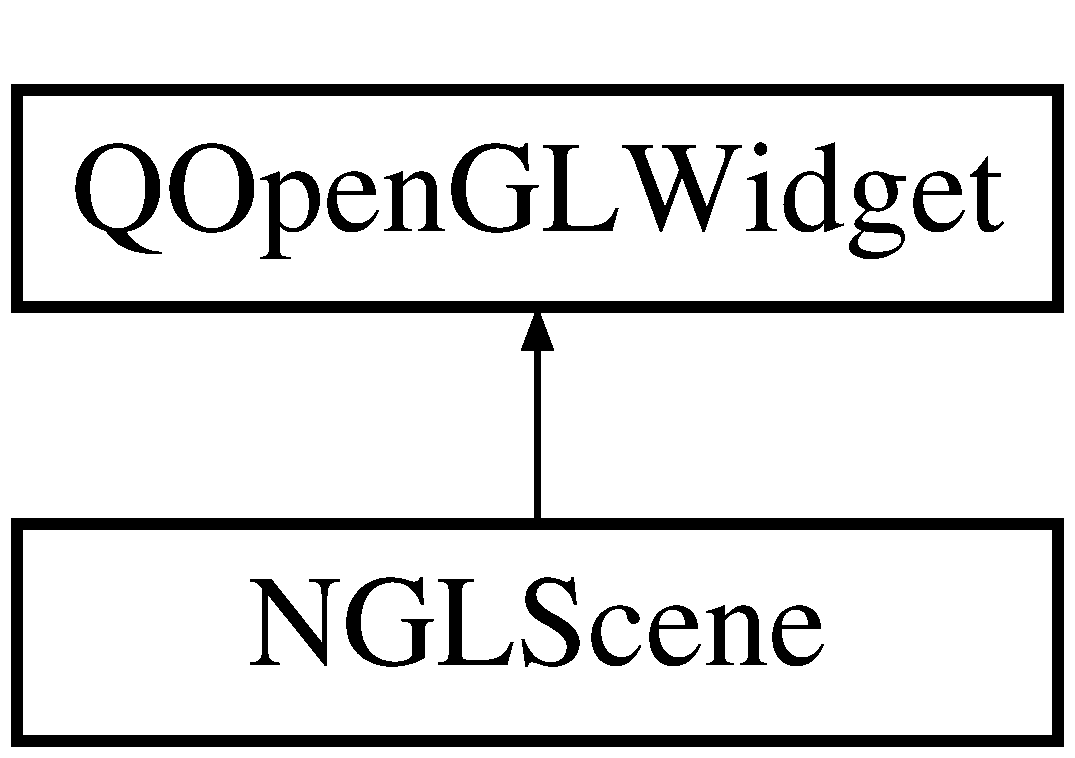
\includegraphics[height=2.000000cm]{classNGLScene}
\end{center}
\end{figure}
\subsection*{Public Slots}
\begin{DoxyCompactItemize}
\item 
\hypertarget{classNGLScene_aa484c5103aa3829f0495f13bc8fb8482}{void \hyperlink{classNGLScene_aa484c5103aa3829f0495f13bc8fb8482}{load\-Mesh} ()}\label{classNGLScene_aa484c5103aa3829f0495f13bc8fb8482}

\begin{DoxyCompactList}\small\item\em load\-Mesh Loads a mesh, generates a \hyperlink{classSBVH}{S\-B\-V\-H} acceleration structure for it and passes the data the renderer \end{DoxyCompactList}\item 
\hypertarget{classNGLScene_a954a5eb1691e9828aed8d180a42575eb}{void \hyperlink{classNGLScene_a954a5eb1691e9828aed8d180a42575eb}{load\-H\-D\-R} ()}\label{classNGLScene_a954a5eb1691e9828aed8d180a42575eb}

\begin{DoxyCompactList}\small\item\em load\-H\-D\-R Loads an E\-X\-R and passes the data to the renderer \end{DoxyCompactList}\item 
\hypertarget{classNGLScene_a6efc515d291011cd581480a4a4916e5c}{void \hyperlink{classNGLScene_a6efc515d291011cd581480a4a4916e5c}{load\-B\-R\-D\-F} ()}\label{classNGLScene_a6efc515d291011cd581480a4a4916e5c}

\begin{DoxyCompactList}\small\item\em load\-B\-R\-D\-F Loads M\-E\-R\-L B\-R\-D\-F data and passes it to the renderer \end{DoxyCompactList}\item 
void \hyperlink{classNGLScene_abee07cadf7d9342fa40e68576130b2ad}{use\-B\-R\-D\-F} (const bool \&\-\_\-val)
\begin{DoxyCompactList}\small\item\em use\-B\-R\-D\-F Passes an U\-I signal to the renderer whether to use the B\-R\-D\-F data or not \end{DoxyCompactList}\item 
void \hyperlink{classNGLScene_a2e02406936e4cbd1756301836533e476}{use\-Example\-Sphere} (const bool \&\-\_\-val)
\begin{DoxyCompactList}\small\item\em use\-Example\-Sphere Passes an U\-I signal to the renderer whether to use an example sphere \end{DoxyCompactList}\item 
void \hyperlink{classNGLScene_aa6b13cd9be96a0fb83224eca63ca9ca1}{use\-Cornell\-Env} (const bool \&\-\_\-val)
\begin{DoxyCompactList}\small\item\em use\-Cornell\-Env Passes an U\-I signal to the renderer whether to use the Cornell box or an H\-D\-R\-I environment \end{DoxyCompactList}\item 
\hypertarget{classNGLScene_a17174c3763736bc8e5de55eb551e91dd}{void \hyperlink{classNGLScene_a17174c3763736bc8e5de55eb551e91dd}{load\-Diffuse} ()}\label{classNGLScene_a17174c3763736bc8e5de55eb551e91dd}

\begin{DoxyCompactList}\small\item\em load\-Diffuse Pass through function to load in a diffuse texture \end{DoxyCompactList}\item 
\hypertarget{classNGLScene_a9e19c5d383822133d99d2c5359406ee8}{void \hyperlink{classNGLScene_a9e19c5d383822133d99d2c5359406ee8}{load\-Normal} ()}\label{classNGLScene_a9e19c5d383822133d99d2c5359406ee8}

\begin{DoxyCompactList}\small\item\em load\-Normal Pass through function to load in a normal texture \end{DoxyCompactList}\item 
\hypertarget{classNGLScene_a660fd684af6638405e2acefbd85c5508}{void \hyperlink{classNGLScene_a660fd684af6638405e2acefbd85c5508}{load\-Specular} ()}\label{classNGLScene_a660fd684af6638405e2acefbd85c5508}

\begin{DoxyCompactList}\small\item\em load\-Specular Pass through function to load in a specular texture \end{DoxyCompactList}\item 
void \hyperlink{classNGLScene_ae4242aaaa2dc60172a46d463621bb8a2}{change\-Fov} (const int \&\-\_\-new\-Fov)
\begin{DoxyCompactList}\small\item\em change\-Fov Updates the F\-O\-V from the U\-I to the renderer \end{DoxyCompactList}\item 
void \hyperlink{classNGLScene_a20182f83391c960705b3de402b064386}{change\-Fresnel\-Coef} (const int \&\-\_\-new\-Val)
\begin{DoxyCompactList}\small\item\em change\-Fresnel\-Coef Updates the fresnel coef from the U\-I to the renderer \end{DoxyCompactList}\item 
void \hyperlink{classNGLScene_ae4c42b19a25e4b43b804202c79c89bc2}{change\-Fresnel\-Power} (const int \&\-\_\-new\-Val)
\begin{DoxyCompactList}\small\item\em change\-Fresnel\-Power Updates the fresnel power from the U\-I to the renderer \end{DoxyCompactList}\item 
void \hyperlink{classNGLScene_a51c28cc0b7e022828003de95f1ea5523}{toggle\-F\-X\-A\-A} (const bool \&\-\_\-enabled)
\begin{DoxyCompactList}\small\item\em toggle\-F\-X\-A\-A Enable/disable F\-X\-A\-A based on the U\-I input \end{DoxyCompactList}\item 
void \hyperlink{classNGLScene_aebb9ebf6d1523bb0669da8c84113c943}{fxaa\-Sharpness} (const int \&\-\_\-new\-Val)
\begin{DoxyCompactList}\small\item\em fxaa\-Sharpness Updates the F\-X\-A\-A sharpness shader uniform \end{DoxyCompactList}\item 
void \hyperlink{classNGLScene_aa45b262a9ee4669f842a9ebf3716d338}{fxaa\-Subpix\-Quality} (const int \&\-\_\-new\-Val)
\begin{DoxyCompactList}\small\item\em fxaa\-Subpix\-Quality Updates the F\-X\-A\-A subpixel quality shader uniform \end{DoxyCompactList}\item 
void \hyperlink{classNGLScene_afeaf7b8feeedbed5ead3db706a07c9b6}{fxaa\-Edge\-Threshold} (const int \&\-\_\-new\-Val)
\begin{DoxyCompactList}\small\item\em fxaa\-Edge\-Threshold Updates the F\-X\-A\-A edge threshold shader uniform \end{DoxyCompactList}\end{DoxyCompactItemize}
\subsection*{Signals}
\begin{DoxyCompactItemize}
\item 
\hypertarget{classNGLScene_ab7b1e32434f2a2c2f0dd1ece6661ca79}{void \hyperlink{classNGLScene_ab7b1e32434f2a2c2f0dd1ece6661ca79}{mesh\-Loaded} (const Q\-String \&)}\label{classNGLScene_ab7b1e32434f2a2c2f0dd1ece6661ca79}

\begin{DoxyCompactList}\small\item\em mesh\-Loaded Signals the U\-I that a mesh has been loaded successfully \end{DoxyCompactList}\item 
\hypertarget{classNGLScene_acaf032b837c09feaf534779a216923cd}{void \hyperlink{classNGLScene_acaf032b837c09feaf534779a216923cd}{texture\-Loaded} (const Q\-String \&, const unsigned int \&)}\label{classNGLScene_acaf032b837c09feaf534779a216923cd}

\begin{DoxyCompactList}\small\item\em texture\-Loaded Signals the U\-I that a texture has been loaded successfully \end{DoxyCompactList}\item 
\hypertarget{classNGLScene_a219b32b4e420ecf8510b282e39f6c954}{void \hyperlink{classNGLScene_a219b32b4e420ecf8510b282e39f6c954}{brdf\-Loaded} (const Q\-String \&)}\label{classNGLScene_a219b32b4e420ecf8510b282e39f6c954}

\begin{DoxyCompactList}\small\item\em brdf\-Loaded Signals the U\-I that M\-E\-R\-L B\-R\-D\-F data has been loaded successfully \end{DoxyCompactList}\item 
\hypertarget{classNGLScene_ac31e02ed631b1d67aa1d43d31bb8e4fe}{void \hyperlink{classNGLScene_ac31e02ed631b1d67aa1d43d31bb8e4fe}{H\-D\-R\-I\-Loaded} (const Q\-String \&)}\label{classNGLScene_ac31e02ed631b1d67aa1d43d31bb8e4fe}

\begin{DoxyCompactList}\small\item\em H\-D\-R\-I\-Loaded Signals the U\-I that a H\-D\-R\-I map has been loaded successfully. \end{DoxyCompactList}\end{DoxyCompactItemize}
\subsection*{Public Member Functions}
\begin{DoxyCompactItemize}
\item 
\hyperlink{classNGLScene_a15c28d86bb9083dee9fa92b6941b76f1}{N\-G\-L\-Scene} (Q\-Widget $\ast$\-\_\-parent=nullptr)
\begin{DoxyCompactList}\small\item\em ctor for our N\-G\-L drawing class \end{DoxyCompactList}\item 
\hypertarget{classNGLScene_abda05d130945833bfbb6bad8d619f7f5}{\hyperlink{classNGLScene_abda05d130945833bfbb6bad8d619f7f5}{$\sim$\-N\-G\-L\-Scene} ()}\label{classNGLScene_abda05d130945833bfbb6bad8d619f7f5}

\begin{DoxyCompactList}\small\item\em dtor must close down ngl and release Open\-G\-L resources \end{DoxyCompactList}\item 
void \hyperlink{classNGLScene_aab2b866db534d286a56cc2240ed98790}{initialize\-G\-L} ()
\begin{DoxyCompactList}\small\item\em the initialize class is called once when the window is created and we have a valid G\-L context \end{DoxyCompactList}\item 
\hypertarget{classNGLScene_a37bec65bfba7b7a717d803d369221e2d}{void \hyperlink{classNGLScene_a37bec65bfba7b7a717d803d369221e2d}{paint\-G\-L} ()}\label{classNGLScene_a37bec65bfba7b7a717d803d369221e2d}

\begin{DoxyCompactList}\small\item\em this is called everytime we want to draw the scene \end{DoxyCompactList}\item 
\hypertarget{classNGLScene_ac228e4d41afa023733b163d2128c78fb}{void {\bfseries change\-Render\-Channel} ()}\label{classNGLScene_ac228e4d41afa023733b163d2128c78fb}

\end{DoxyCompactItemize}


\subsection{Detailed Description}
our main glwindow widget for N\-G\-L applications all drawing elements are put in this file 

\subsection{Constructor \& Destructor Documentation}
\hypertarget{classNGLScene_a15c28d86bb9083dee9fa92b6941b76f1}{\index{N\-G\-L\-Scene@{N\-G\-L\-Scene}!N\-G\-L\-Scene@{N\-G\-L\-Scene}}
\index{N\-G\-L\-Scene@{N\-G\-L\-Scene}!NGLScene@{N\-G\-L\-Scene}}
\subsubsection[{N\-G\-L\-Scene}]{\setlength{\rightskip}{0pt plus 5cm}N\-G\-L\-Scene\-::\-N\-G\-L\-Scene (
\begin{DoxyParamCaption}
\item[{Q\-Widget $\ast$}]{\-\_\-parent = {\ttfamily nullptr}}
\end{DoxyParamCaption}
)}}\label{classNGLScene_a15c28d86bb9083dee9fa92b6941b76f1}


ctor for our N\-G\-L drawing class 


\begin{DoxyParams}[1]{Parameters}
\mbox{\tt in}  & {\em parent} & the parent window to the class \\
\hline
\end{DoxyParams}


\subsection{Member Function Documentation}
\hypertarget{classNGLScene_ae4242aaaa2dc60172a46d463621bb8a2}{\index{N\-G\-L\-Scene@{N\-G\-L\-Scene}!change\-Fov@{change\-Fov}}
\index{change\-Fov@{change\-Fov}!NGLScene@{N\-G\-L\-Scene}}
\subsubsection[{change\-Fov}]{\setlength{\rightskip}{0pt plus 5cm}void N\-G\-L\-Scene\-::change\-Fov (
\begin{DoxyParamCaption}
\item[{const int \&}]{\-\_\-new\-Fov}
\end{DoxyParamCaption}
)\hspace{0.3cm}{\ttfamily [slot]}}}\label{classNGLScene_ae4242aaaa2dc60172a46d463621bb8a2}


change\-Fov Updates the F\-O\-V from the U\-I to the renderer 


\begin{DoxyParams}{Parameters}
{\em \-\_\-new\-Fov} & New field of view to be used \\
\hline
\end{DoxyParams}
\hypertarget{classNGLScene_a20182f83391c960705b3de402b064386}{\index{N\-G\-L\-Scene@{N\-G\-L\-Scene}!change\-Fresnel\-Coef@{change\-Fresnel\-Coef}}
\index{change\-Fresnel\-Coef@{change\-Fresnel\-Coef}!NGLScene@{N\-G\-L\-Scene}}
\subsubsection[{change\-Fresnel\-Coef}]{\setlength{\rightskip}{0pt plus 5cm}void N\-G\-L\-Scene\-::change\-Fresnel\-Coef (
\begin{DoxyParamCaption}
\item[{const int \&}]{\-\_\-new\-Val}
\end{DoxyParamCaption}
)\hspace{0.3cm}{\ttfamily [slot]}}}\label{classNGLScene_a20182f83391c960705b3de402b064386}


change\-Fresnel\-Coef Updates the fresnel coef from the U\-I to the renderer 


\begin{DoxyParams}{Parameters}
{\em \-\_\-new\-Val} & New fresnel coef \\
\hline
\end{DoxyParams}
\hypertarget{classNGLScene_ae4c42b19a25e4b43b804202c79c89bc2}{\index{N\-G\-L\-Scene@{N\-G\-L\-Scene}!change\-Fresnel\-Power@{change\-Fresnel\-Power}}
\index{change\-Fresnel\-Power@{change\-Fresnel\-Power}!NGLScene@{N\-G\-L\-Scene}}
\subsubsection[{change\-Fresnel\-Power}]{\setlength{\rightskip}{0pt plus 5cm}void N\-G\-L\-Scene\-::change\-Fresnel\-Power (
\begin{DoxyParamCaption}
\item[{const int \&}]{\-\_\-new\-Val}
\end{DoxyParamCaption}
)\hspace{0.3cm}{\ttfamily [slot]}}}\label{classNGLScene_ae4c42b19a25e4b43b804202c79c89bc2}


change\-Fresnel\-Power Updates the fresnel power from the U\-I to the renderer 


\begin{DoxyParams}{Parameters}
{\em \-\_\-new\-Val} & New fresnel power \\
\hline
\end{DoxyParams}
\hypertarget{classNGLScene_afeaf7b8feeedbed5ead3db706a07c9b6}{\index{N\-G\-L\-Scene@{N\-G\-L\-Scene}!fxaa\-Edge\-Threshold@{fxaa\-Edge\-Threshold}}
\index{fxaa\-Edge\-Threshold@{fxaa\-Edge\-Threshold}!NGLScene@{N\-G\-L\-Scene}}
\subsubsection[{fxaa\-Edge\-Threshold}]{\setlength{\rightskip}{0pt plus 5cm}void N\-G\-L\-Scene\-::fxaa\-Edge\-Threshold (
\begin{DoxyParamCaption}
\item[{const int \&}]{\-\_\-new\-Val}
\end{DoxyParamCaption}
)\hspace{0.3cm}{\ttfamily [inline]}, {\ttfamily [slot]}}}\label{classNGLScene_afeaf7b8feeedbed5ead3db706a07c9b6}


fxaa\-Edge\-Threshold Updates the F\-X\-A\-A edge threshold shader uniform 


\begin{DoxyParams}{Parameters}
{\em \-\_\-new\-Val} & New F\-X\-A\-A edge threshold value \\
\hline
\end{DoxyParams}
\hypertarget{classNGLScene_aebb9ebf6d1523bb0669da8c84113c943}{\index{N\-G\-L\-Scene@{N\-G\-L\-Scene}!fxaa\-Sharpness@{fxaa\-Sharpness}}
\index{fxaa\-Sharpness@{fxaa\-Sharpness}!NGLScene@{N\-G\-L\-Scene}}
\subsubsection[{fxaa\-Sharpness}]{\setlength{\rightskip}{0pt plus 5cm}void N\-G\-L\-Scene\-::fxaa\-Sharpness (
\begin{DoxyParamCaption}
\item[{const int \&}]{\-\_\-new\-Val}
\end{DoxyParamCaption}
)\hspace{0.3cm}{\ttfamily [inline]}, {\ttfamily [slot]}}}\label{classNGLScene_aebb9ebf6d1523bb0669da8c84113c943}


fxaa\-Sharpness Updates the F\-X\-A\-A sharpness shader uniform 


\begin{DoxyParams}{Parameters}
{\em \-\_\-new\-Val} & New F\-X\-A\-A sharpness value \\
\hline
\end{DoxyParams}
\hypertarget{classNGLScene_aa45b262a9ee4669f842a9ebf3716d338}{\index{N\-G\-L\-Scene@{N\-G\-L\-Scene}!fxaa\-Subpix\-Quality@{fxaa\-Subpix\-Quality}}
\index{fxaa\-Subpix\-Quality@{fxaa\-Subpix\-Quality}!NGLScene@{N\-G\-L\-Scene}}
\subsubsection[{fxaa\-Subpix\-Quality}]{\setlength{\rightskip}{0pt plus 5cm}void N\-G\-L\-Scene\-::fxaa\-Subpix\-Quality (
\begin{DoxyParamCaption}
\item[{const int \&}]{\-\_\-new\-Val}
\end{DoxyParamCaption}
)\hspace{0.3cm}{\ttfamily [inline]}, {\ttfamily [slot]}}}\label{classNGLScene_aa45b262a9ee4669f842a9ebf3716d338}


fxaa\-Subpix\-Quality Updates the F\-X\-A\-A subpixel quality shader uniform 


\begin{DoxyParams}{Parameters}
{\em \-\_\-new\-Val} & New F\-X\-A\-A subpixel quality value \\
\hline
\end{DoxyParams}
\hypertarget{classNGLScene_aab2b866db534d286a56cc2240ed98790}{\index{N\-G\-L\-Scene@{N\-G\-L\-Scene}!initialize\-G\-L@{initialize\-G\-L}}
\index{initialize\-G\-L@{initialize\-G\-L}!NGLScene@{N\-G\-L\-Scene}}
\subsubsection[{initialize\-G\-L}]{\setlength{\rightskip}{0pt plus 5cm}void N\-G\-L\-Scene\-::initialize\-G\-L (
\begin{DoxyParamCaption}
{}
\end{DoxyParamCaption}
)}}\label{classNGLScene_aab2b866db534d286a56cc2240ed98790}


the initialize class is called once when the window is created and we have a valid G\-L context 

use this to setup any default G\-L stuff Load in the normal screen quad and F\-X\-A\-A shaders \hypertarget{classNGLScene_a51c28cc0b7e022828003de95f1ea5523}{\index{N\-G\-L\-Scene@{N\-G\-L\-Scene}!toggle\-F\-X\-A\-A@{toggle\-F\-X\-A\-A}}
\index{toggle\-F\-X\-A\-A@{toggle\-F\-X\-A\-A}!NGLScene@{N\-G\-L\-Scene}}
\subsubsection[{toggle\-F\-X\-A\-A}]{\setlength{\rightskip}{0pt plus 5cm}void N\-G\-L\-Scene\-::toggle\-F\-X\-A\-A (
\begin{DoxyParamCaption}
\item[{const bool \&}]{\-\_\-enabled}
\end{DoxyParamCaption}
)\hspace{0.3cm}{\ttfamily [inline]}, {\ttfamily [slot]}}}\label{classNGLScene_a51c28cc0b7e022828003de95f1ea5523}


toggle\-F\-X\-A\-A Enable/disable F\-X\-A\-A based on the U\-I input 


\begin{DoxyParams}{Parameters}
{\em \-\_\-enabled} & Whether to use F\-X\-A\-A or not \\
\hline
\end{DoxyParams}
\hypertarget{classNGLScene_abee07cadf7d9342fa40e68576130b2ad}{\index{N\-G\-L\-Scene@{N\-G\-L\-Scene}!use\-B\-R\-D\-F@{use\-B\-R\-D\-F}}
\index{use\-B\-R\-D\-F@{use\-B\-R\-D\-F}!NGLScene@{N\-G\-L\-Scene}}
\subsubsection[{use\-B\-R\-D\-F}]{\setlength{\rightskip}{0pt plus 5cm}void N\-G\-L\-Scene\-::use\-B\-R\-D\-F (
\begin{DoxyParamCaption}
\item[{const bool \&}]{\-\_\-val}
\end{DoxyParamCaption}
)\hspace{0.3cm}{\ttfamily [slot]}}}\label{classNGLScene_abee07cadf7d9342fa40e68576130b2ad}


use\-B\-R\-D\-F Passes an U\-I signal to the renderer whether to use the B\-R\-D\-F data or not 


\begin{DoxyParams}{Parameters}
{\em \-\_\-val} & Whether to use B\-R\-D\-F or not \\
\hline
\end{DoxyParams}
\hypertarget{classNGLScene_aa6b13cd9be96a0fb83224eca63ca9ca1}{\index{N\-G\-L\-Scene@{N\-G\-L\-Scene}!use\-Cornell\-Env@{use\-Cornell\-Env}}
\index{use\-Cornell\-Env@{use\-Cornell\-Env}!NGLScene@{N\-G\-L\-Scene}}
\subsubsection[{use\-Cornell\-Env}]{\setlength{\rightskip}{0pt plus 5cm}void N\-G\-L\-Scene\-::use\-Cornell\-Env (
\begin{DoxyParamCaption}
\item[{const bool \&}]{\-\_\-val}
\end{DoxyParamCaption}
)\hspace{0.3cm}{\ttfamily [slot]}}}\label{classNGLScene_aa6b13cd9be96a0fb83224eca63ca9ca1}


use\-Cornell\-Env Passes an U\-I signal to the renderer whether to use the Cornell box or an H\-D\-R\-I environment 


\begin{DoxyParams}{Parameters}
{\em \-\_\-val} & \\
\hline
\end{DoxyParams}
\hypertarget{classNGLScene_a2e02406936e4cbd1756301836533e476}{\index{N\-G\-L\-Scene@{N\-G\-L\-Scene}!use\-Example\-Sphere@{use\-Example\-Sphere}}
\index{use\-Example\-Sphere@{use\-Example\-Sphere}!NGLScene@{N\-G\-L\-Scene}}
\subsubsection[{use\-Example\-Sphere}]{\setlength{\rightskip}{0pt plus 5cm}void N\-G\-L\-Scene\-::use\-Example\-Sphere (
\begin{DoxyParamCaption}
\item[{const bool \&}]{\-\_\-val}
\end{DoxyParamCaption}
)\hspace{0.3cm}{\ttfamily [slot]}}}\label{classNGLScene_a2e02406936e4cbd1756301836533e476}


use\-Example\-Sphere Passes an U\-I signal to the renderer whether to use an example sphere 


\begin{DoxyParams}{Parameters}
{\em \-\_\-val} & Whether to use the example shere or not \\
\hline
\end{DoxyParams}


The documentation for this class was generated from the following files\-:\begin{DoxyCompactItemize}
\item 
include/\hyperlink{NGLScene_8h}{N\-G\-L\-Scene.\-h}\item 
moc/moc\-\_\-\-N\-G\-L\-Scene.\-cpp\item 
src/\hyperlink{NGLScene_8cpp}{N\-G\-L\-Scene.\-cpp}\item 
src/N\-G\-L\-Scene\-Mouse\-Controls.\-cpp\end{DoxyCompactItemize}

\hypertarget{structqt__meta__stringdata__MainWindow__t}{\section{qt\-\_\-meta\-\_\-stringdata\-\_\-\-Main\-Window\-\_\-t Struct Reference}
\label{structqt__meta__stringdata__MainWindow__t}\index{qt\-\_\-meta\-\_\-stringdata\-\_\-\-Main\-Window\-\_\-t@{qt\-\_\-meta\-\_\-stringdata\-\_\-\-Main\-Window\-\_\-t}}
}
\subsection*{Public Attributes}
\begin{DoxyCompactItemize}
\item 
\hypertarget{structqt__meta__stringdata__MainWindow__t_afd67093eee085680898ad79aa678a6fe}{Q\-Byte\-Array\-Data {\bfseries data} \mbox{[}19\mbox{]}}\label{structqt__meta__stringdata__MainWindow__t_afd67093eee085680898ad79aa678a6fe}

\item 
\hypertarget{structqt__meta__stringdata__MainWindow__t_ac66323ffb3afc76c1ebf5d7e96be1b70}{char {\bfseries stringdata0} \mbox{[}245\mbox{]}}\label{structqt__meta__stringdata__MainWindow__t_ac66323ffb3afc76c1ebf5d7e96be1b70}

\end{DoxyCompactItemize}


The documentation for this struct was generated from the following file\-:\begin{DoxyCompactItemize}
\item 
moc/moc\-\_\-mainwindow.\-cpp\end{DoxyCompactItemize}

\hypertarget{structqt__meta__stringdata__NGLScene__t}{\section{qt\-\_\-meta\-\_\-stringdata\-\_\-\-N\-G\-L\-Scene\-\_\-t Struct Reference}
\label{structqt__meta__stringdata__NGLScene__t}\index{qt\-\_\-meta\-\_\-stringdata\-\_\-\-N\-G\-L\-Scene\-\_\-t@{qt\-\_\-meta\-\_\-stringdata\-\_\-\-N\-G\-L\-Scene\-\_\-t}}
}
\subsection*{Public Attributes}
\begin{DoxyCompactItemize}
\item 
\hypertarget{structqt__meta__stringdata__NGLScene__t_a728fa62392c3b5b85ed1cd408bc3f0e2}{Q\-Byte\-Array\-Data {\bfseries data} \mbox{[}26\mbox{]}}\label{structqt__meta__stringdata__NGLScene__t_a728fa62392c3b5b85ed1cd408bc3f0e2}

\item 
\hypertarget{structqt__meta__stringdata__NGLScene__t_a3c692b71b22d5950a17b11a0cd819cb0}{char {\bfseries stringdata0} \mbox{[}296\mbox{]}}\label{structqt__meta__stringdata__NGLScene__t_a3c692b71b22d5950a17b11a0cd819cb0}

\end{DoxyCompactItemize}


The documentation for this struct was generated from the following file\-:\begin{DoxyCompactItemize}
\item 
moc/moc\-\_\-\-N\-G\-L\-Scene.\-cpp\end{DoxyCompactItemize}

\hypertarget{structRay}{\section{Ray Struct Reference}
\label{structRay}\index{Ray@{Ray}}
}


\hyperlink{structRay}{Ray} Simple structure for a ray.  




{\ttfamily \#include $<$Path\-Tracer.\-h$>$}

\subsection*{Public Member Functions}
\begin{DoxyCompactItemize}
\item 
\-\_\-\-\_\-device\-\_\-\-\_\- \hyperlink{structRay_a66ef919841d94eafd0cd66974413dc4e}{Ray} (float4 \-\_\-o, float4 \-\_\-d)
\begin{DoxyCompactList}\small\item\em \hyperlink{structRay}{Ray} Default ctor for a ray. \end{DoxyCompactList}\end{DoxyCompactItemize}
\subsection*{Public Attributes}
\begin{DoxyCompactItemize}
\item 
\hypertarget{structRay_a6737aa9524fe3ff15ab2f52772477527}{float4 \hyperlink{structRay_a6737aa9524fe3ff15ab2f52772477527}{m\-\_\-origin}}\label{structRay_a6737aa9524fe3ff15ab2f52772477527}

\begin{DoxyCompactList}\small\item\em m\-\_\-origin Origin of the current ray \end{DoxyCompactList}\item 
\hypertarget{structRay_add4cc30ec7877e3e44713a21d189e4d1}{float4 \hyperlink{structRay_add4cc30ec7877e3e44713a21d189e4d1}{m\-\_\-dir}}\label{structRay_add4cc30ec7877e3e44713a21d189e4d1}

\begin{DoxyCompactList}\small\item\em m\-\_\-dir Direction of the ray \end{DoxyCompactList}\end{DoxyCompactItemize}


\subsection{Detailed Description}
\hyperlink{structRay}{Ray} Simple structure for a ray. 

\subsection{Constructor \& Destructor Documentation}
\hypertarget{structRay_a66ef919841d94eafd0cd66974413dc4e}{\index{Ray@{Ray}!Ray@{Ray}}
\index{Ray@{Ray}!Ray@{Ray}}
\subsubsection[{Ray}]{\setlength{\rightskip}{0pt plus 5cm}\-\_\-\-\_\-device\-\_\-\-\_\- Ray\-::\-Ray (
\begin{DoxyParamCaption}
\item[{float4}]{\-\_\-o, }
\item[{float4}]{\-\_\-d}
\end{DoxyParamCaption}
)\hspace{0.3cm}{\ttfamily [inline]}}}\label{structRay_a66ef919841d94eafd0cd66974413dc4e}


\hyperlink{structRay}{Ray} Default ctor for a ray. 


\begin{DoxyParams}{Parameters}
{\em \-\_\-o} & Origin of the ray \\
\hline
{\em \-\_\-d} & Direction of the ray \\
\hline
\end{DoxyParams}


The documentation for this struct was generated from the following files\-:\begin{DoxyCompactItemize}
\item 
cl/include/\hyperlink{PathTracer_8h}{Path\-Tracer.\-h}\item 
cuda/include/\hyperlink{RayIntersection_8cuh}{Ray\-Intersection.\-cuh}\end{DoxyCompactItemize}

\hypertarget{classSBVH}{\section{S\-B\-V\-H Class Reference}
\label{classSBVH}\index{S\-B\-V\-H@{S\-B\-V\-H}}
}


The \hyperlink{classSBVH}{S\-B\-V\-H} class The class builds the acceleration structure when given a vector of triangles and vertices.  




{\ttfamily \#include $<$S\-B\-V\-H.\-h$>$}

\subsection*{Public Member Functions}
\begin{DoxyCompactItemize}
\item 
\hyperlink{classSBVH_ae0fdf31d3d402ea09c63d261977f4192}{S\-B\-V\-H} (\hyperlink{structvHTriangle}{v\-H\-Triangle} $\ast$\-\_\-triangles, \hyperlink{structvHVert}{v\-H\-Vert} $\ast$\-\_\-verts, unsigned int \-\_\-num\-Tris)
\begin{DoxyCompactList}\small\item\em \hyperlink{classSBVH}{S\-B\-V\-H} Default ctor for the \hyperlink{classSBVH}{S\-B\-V\-H}, calculates the \hyperlink{classAABB}{A\-A\-B\-B} for the root node and builds the triangle reference vector and starts building the acceleration structure from the root. \end{DoxyCompactList}\item 
\hyperlink{classBVHNode}{B\-V\-H\-Node} $\ast$ \hyperlink{classSBVH_a7d65b77c45768401d3f7740698f01164}{get\-Root} () const 
\begin{DoxyCompactList}\small\item\em get\-Root Get the root node \end{DoxyCompactList}\item 
unsigned int \hyperlink{classSBVH_af7a06b4c346366f15b15730f10346c10}{get\-Tri\-Index} (const unsigned int \&\-\_\-i) const 
\begin{DoxyCompactList}\small\item\em get\-Tri\-Index Get the index of a triangle from the triangle reference stack \end{DoxyCompactList}\item 
unsigned int \hyperlink{classSBVH_ac30b20f84eebea2a929e2f201936e62f}{get\-Node\-Count} ()
\begin{DoxyCompactList}\small\item\em get\-Node\-Count Get the number of nodes in the final acceleration structure \end{DoxyCompactList}\end{DoxyCompactItemize}


\subsection{Detailed Description}
The \hyperlink{classSBVH}{S\-B\-V\-H} class The class builds the acceleration structure when given a vector of triangles and vertices. 

\subsection{Constructor \& Destructor Documentation}
\hypertarget{classSBVH_ae0fdf31d3d402ea09c63d261977f4192}{\index{S\-B\-V\-H@{S\-B\-V\-H}!S\-B\-V\-H@{S\-B\-V\-H}}
\index{S\-B\-V\-H@{S\-B\-V\-H}!SBVH@{S\-B\-V\-H}}
\subsubsection[{S\-B\-V\-H}]{\setlength{\rightskip}{0pt plus 5cm}S\-B\-V\-H\-::\-S\-B\-V\-H (
\begin{DoxyParamCaption}
\item[{{\bf v\-H\-Triangle} $\ast$}]{\-\_\-triangles, }
\item[{{\bf v\-H\-Vert} $\ast$}]{\-\_\-verts, }
\item[{unsigned int}]{\-\_\-num\-Tris}
\end{DoxyParamCaption}
)}}\label{classSBVH_ae0fdf31d3d402ea09c63d261977f4192}


\hyperlink{classSBVH}{S\-B\-V\-H} Default ctor for the \hyperlink{classSBVH}{S\-B\-V\-H}, calculates the \hyperlink{classAABB}{A\-A\-B\-B} for the root node and builds the triangle reference vector and starts building the acceleration structure from the root. 


\begin{DoxyParams}{Parameters}
{\em \-\_\-triangles} & Triangles of the mesh \\
\hline
{\em \-\_\-verts} & Vertices of the mesh \\
\hline
{\em \-\_\-num\-Tris} & Number of triangles in the mesh \\
\hline
\end{DoxyParams}


\subsection{Member Function Documentation}
\hypertarget{classSBVH_ac30b20f84eebea2a929e2f201936e62f}{\index{S\-B\-V\-H@{S\-B\-V\-H}!get\-Node\-Count@{get\-Node\-Count}}
\index{get\-Node\-Count@{get\-Node\-Count}!SBVH@{S\-B\-V\-H}}
\subsubsection[{get\-Node\-Count}]{\setlength{\rightskip}{0pt plus 5cm}unsigned int S\-B\-V\-H\-::get\-Node\-Count (
\begin{DoxyParamCaption}
{}
\end{DoxyParamCaption}
)\hspace{0.3cm}{\ttfamily [inline]}}}\label{classSBVH_ac30b20f84eebea2a929e2f201936e62f}


get\-Node\-Count Get the number of nodes in the final acceleration structure 

\begin{DoxyReturn}{Returns}
Number of nodes in the structure 
\end{DoxyReturn}
\hypertarget{classSBVH_a7d65b77c45768401d3f7740698f01164}{\index{S\-B\-V\-H@{S\-B\-V\-H}!get\-Root@{get\-Root}}
\index{get\-Root@{get\-Root}!SBVH@{S\-B\-V\-H}}
\subsubsection[{get\-Root}]{\setlength{\rightskip}{0pt plus 5cm}{\bf B\-V\-H\-Node}$\ast$ S\-B\-V\-H\-::get\-Root (
\begin{DoxyParamCaption}
{}
\end{DoxyParamCaption}
) const\hspace{0.3cm}{\ttfamily [inline]}}}\label{classSBVH_a7d65b77c45768401d3f7740698f01164}


get\-Root Get the root node 

\begin{DoxyReturn}{Returns}
The root node 
\end{DoxyReturn}
\hypertarget{classSBVH_af7a06b4c346366f15b15730f10346c10}{\index{S\-B\-V\-H@{S\-B\-V\-H}!get\-Tri\-Index@{get\-Tri\-Index}}
\index{get\-Tri\-Index@{get\-Tri\-Index}!SBVH@{S\-B\-V\-H}}
\subsubsection[{get\-Tri\-Index}]{\setlength{\rightskip}{0pt plus 5cm}unsigned int S\-B\-V\-H\-::get\-Tri\-Index (
\begin{DoxyParamCaption}
\item[{const unsigned int \&}]{\-\_\-i}
\end{DoxyParamCaption}
) const\hspace{0.3cm}{\ttfamily [inline]}}}\label{classSBVH_af7a06b4c346366f15b15730f10346c10}


get\-Tri\-Index Get the index of a triangle from the triangle reference stack 


\begin{DoxyParams}{Parameters}
{\em \-\_\-i} & Index to the reference stack \\
\hline
\end{DoxyParams}
\begin{DoxyReturn}{Returns}
Index of the triangle referenced 
\end{DoxyReturn}


The documentation for this class was generated from the following files\-:\begin{DoxyCompactItemize}
\item 
include/\hyperlink{SBVH_8h}{S\-B\-V\-H.\-h}\item 
src/S\-B\-V\-H.\-cpp\end{DoxyCompactItemize}

\hypertarget{structSphere}{\section{Sphere Struct Reference}
\label{structSphere}\index{Sphere@{Sphere}}
}


\hyperlink{structSphere}{Sphere} Simple sphere structure, used for the example sphere, cornell box scene and few others.  




{\ttfamily \#include $<$Path\-Tracer.\-h$>$}

\subsection*{Public Member Functions}
\begin{DoxyCompactItemize}
\item 
\-\_\-\-\_\-device\-\_\-\-\_\- float \hyperlink{structSphere_aff7f40563a36da274224cce2df67c5bb}{intersect} (const \hyperlink{structRay}{Ray} $\ast$\-\_\-r) const 
\begin{DoxyCompactList}\small\item\em intersect Check if a given ray intersects with the sphere \end{DoxyCompactList}\end{DoxyCompactItemize}
\subsection*{Public Attributes}
\begin{DoxyCompactItemize}
\item 
\hypertarget{structSphere_a2476da8402053c022436054f108bf8aa}{float \hyperlink{structSphere_a2476da8402053c022436054f108bf8aa}{m\-\_\-r}}\label{structSphere_a2476da8402053c022436054f108bf8aa}

\begin{DoxyCompactList}\small\item\em m\-\_\-r Radius of the sphere \end{DoxyCompactList}\item 
\hypertarget{structSphere_a2ab691669ddac359fa0b5ea7b219af26}{float4 \hyperlink{structSphere_a2ab691669ddac359fa0b5ea7b219af26}{m\-\_\-pos}}\label{structSphere_a2ab691669ddac359fa0b5ea7b219af26}

\begin{DoxyCompactList}\small\item\em m\-\_\-pos Position of the sphere \end{DoxyCompactList}\item 
\hypertarget{structSphere_ad64c90d5b23a0af4f9e3bc7d9fce9da4}{float4 \hyperlink{structSphere_ad64c90d5b23a0af4f9e3bc7d9fce9da4}{m\-\_\-emission}}\label{structSphere_ad64c90d5b23a0af4f9e3bc7d9fce9da4}

\begin{DoxyCompactList}\small\item\em m\-\_\-emission Emission of the sphere \end{DoxyCompactList}\item 
\hypertarget{structSphere_aa763efd3f99c9660f450b1925affc014}{float4 \hyperlink{structSphere_aa763efd3f99c9660f450b1925affc014}{m\-\_\-col}}\label{structSphere_aa763efd3f99c9660f450b1925affc014}

\begin{DoxyCompactList}\small\item\em m\-\_\-col Colour of the sphere \end{DoxyCompactList}\item 
\hypertarget{structSphere_a4b7464c09b9fe172751c5689e8f85561}{Refl\-\_\-t \hyperlink{structSphere_a4b7464c09b9fe172751c5689e8f85561}{m\-\_\-refl}}\label{structSphere_a4b7464c09b9fe172751c5689e8f85561}

\begin{DoxyCompactList}\small\item\em m\-\_\-refl Reflective type of the sphere \end{DoxyCompactList}\end{DoxyCompactItemize}


\subsection{Detailed Description}
\hyperlink{structSphere}{Sphere} Simple sphere structure, used for the example sphere, cornell box scene and few others. 

\subsection{Member Function Documentation}
\hypertarget{structSphere_aff7f40563a36da274224cce2df67c5bb}{\index{Sphere@{Sphere}!intersect@{intersect}}
\index{intersect@{intersect}!Sphere@{Sphere}}
\subsubsection[{intersect}]{\setlength{\rightskip}{0pt plus 5cm}\-\_\-\-\_\-device\-\_\-\-\_\- float Sphere\-::intersect (
\begin{DoxyParamCaption}
\item[{const {\bf Ray} $\ast$}]{\-\_\-r}
\end{DoxyParamCaption}
) const\hspace{0.3cm}{\ttfamily [inline]}}}\label{structSphere_aff7f40563a36da274224cce2df67c5bb}


intersect Check if a given ray intersects with the sphere 


\begin{DoxyParams}{Parameters}
{\em \-\_\-r} & \hyperlink{structRay}{Ray} to check against \\
\hline
\end{DoxyParams}
\begin{DoxyReturn}{Returns}
Distance to the intersection if there's on 
\end{DoxyReturn}


The documentation for this struct was generated from the following files\-:\begin{DoxyCompactItemize}
\item 
cl/include/\hyperlink{PathTracer_8h}{Path\-Tracer.\-h}\item 
cuda/src/\hyperlink{PathTracer_8cu}{Path\-Tracer.\-cu}\end{DoxyCompactItemize}

\hypertarget{classUi__MainWindow}{\section{Ui\-\_\-\-Main\-Window Class Reference}
\label{classUi__MainWindow}\index{Ui\-\_\-\-Main\-Window@{Ui\-\_\-\-Main\-Window}}
}
Inheritance diagram for Ui\-\_\-\-Main\-Window\-:\begin{figure}[H]
\begin{center}
\leavevmode
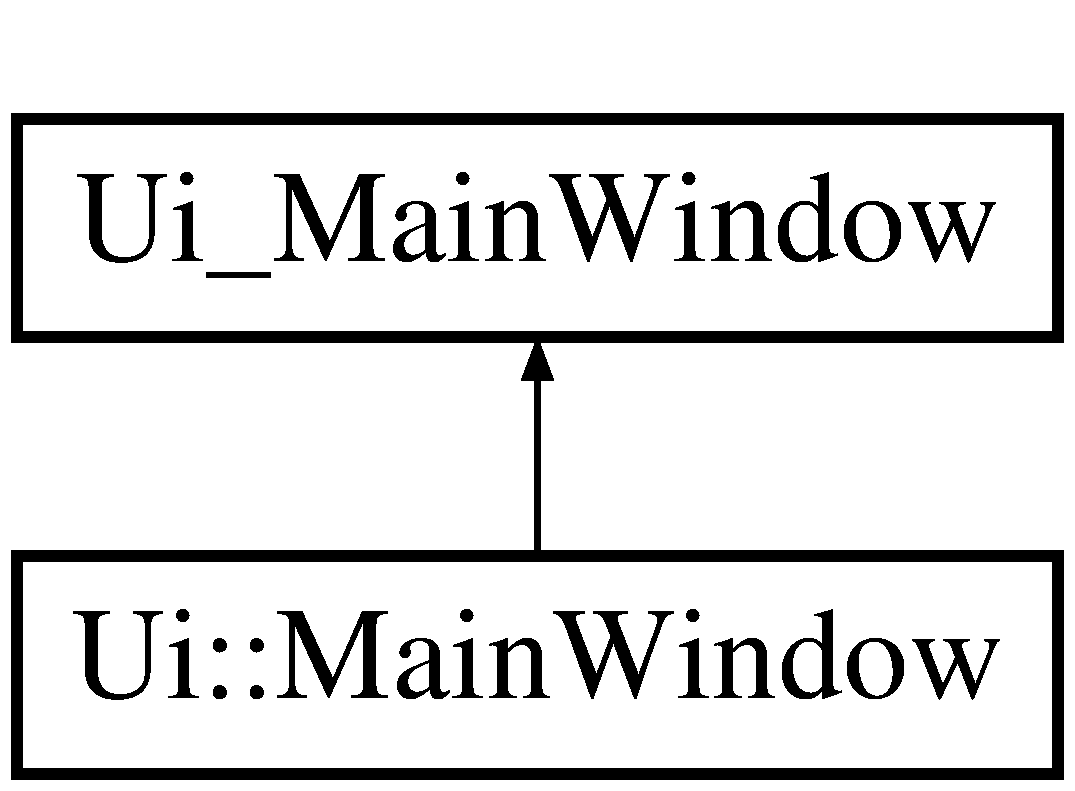
\includegraphics[height=2.000000cm]{classUi__MainWindow}
\end{center}
\end{figure}
\subsection*{Public Member Functions}
\begin{DoxyCompactItemize}
\item 
\hypertarget{classUi__MainWindow_acf4a0872c4c77d8f43a2ec66ed849b58}{void {\bfseries setup\-Ui} (Q\-Main\-Window $\ast$\hyperlink{classMainWindow}{Main\-Window})}\label{classUi__MainWindow_acf4a0872c4c77d8f43a2ec66ed849b58}

\item 
\hypertarget{classUi__MainWindow_a097dd160c3534a204904cb374412c618}{void {\bfseries retranslate\-Ui} (Q\-Main\-Window $\ast$\hyperlink{classMainWindow}{Main\-Window})}\label{classUi__MainWindow_a097dd160c3534a204904cb374412c618}

\end{DoxyCompactItemize}
\subsection*{Public Attributes}
\begin{DoxyCompactItemize}
\item 
\hypertarget{classUi__MainWindow_a30075506c2116c3ed4ff25e07ae75f81}{Q\-Widget $\ast$ {\bfseries central\-Widget}}\label{classUi__MainWindow_a30075506c2116c3ed4ff25e07ae75f81}

\item 
\hypertarget{classUi__MainWindow_a514e971a792abb051013b69a17f0f243}{Q\-Widget $\ast$ {\bfseries m\-\_\-left\-Widget}}\label{classUi__MainWindow_a514e971a792abb051013b69a17f0f243}

\item 
\hypertarget{classUi__MainWindow_a648c7f639f969e69e9b4c4522e209816}{Q\-V\-Box\-Layout $\ast$ {\bfseries m\-\_\-left\-Bar}}\label{classUi__MainWindow_a648c7f639f969e69e9b4c4522e209816}

\item 
\hypertarget{classUi__MainWindow_a64e41af8e7265491439c20298c173280}{Q\-V\-Box\-Layout $\ast$ {\bfseries m\-\_\-scene\-View\-Layout}}\label{classUi__MainWindow_a64e41af8e7265491439c20298c173280}

\item 
\hypertarget{classUi__MainWindow_ad67691cb32591de26ff3bb9234f979ab}{Q\-Label $\ast$ {\bfseries m\-\_\-scene\-Label}}\label{classUi__MainWindow_ad67691cb32591de26ff3bb9234f979ab}

\item 
\hypertarget{classUi__MainWindow_aa75a17fb593180faf058746a3d0f5435}{Q\-Tree\-View $\ast$ {\bfseries m\-\_\-scene\-Tree\-View}}\label{classUi__MainWindow_aa75a17fb593180faf058746a3d0f5435}

\item 
\hypertarget{classUi__MainWindow_ad54952c1d3762f0acf4e7e8e33c36b3d}{Q\-Push\-Button $\ast$ {\bfseries m\-\_\-load\-Mesh\-Btn}}\label{classUi__MainWindow_ad54952c1d3762f0acf4e7e8e33c36b3d}

\item 
\hypertarget{classUi__MainWindow_a711a120cdcd77c5f3030fb2863395364}{Q\-V\-Box\-Layout $\ast$ {\bfseries m\-\_\-env\-Layout}}\label{classUi__MainWindow_a711a120cdcd77c5f3030fb2863395364}

\item 
\hypertarget{classUi__MainWindow_a3f14111eb6b3d622f1dd651ae6e95490}{Q\-Label $\ast$ {\bfseries m\-\_\-env\-Label}}\label{classUi__MainWindow_a3f14111eb6b3d622f1dd651ae6e95490}

\item 
\hypertarget{classUi__MainWindow_a83cf8e88e731ea891bd270a115cdb0e9}{Q\-Radio\-Button $\ast$ {\bfseries m\-\_\-env\-H\-D\-R\-I}}\label{classUi__MainWindow_a83cf8e88e731ea891bd270a115cdb0e9}

\item 
\hypertarget{classUi__MainWindow_af522f7ddf11195c01f36a1578a6d11e4}{Q\-Radio\-Button $\ast$ {\bfseries m\-\_\-env\-Cornell}}\label{classUi__MainWindow_af522f7ddf11195c01f36a1578a6d11e4}

\item 
\hypertarget{classUi__MainWindow_a703ff1513ff398c7b5f61df969aa7ea6}{Q\-Push\-Button $\ast$ {\bfseries m\-\_\-load\-H\-D\-R\-Btn}}\label{classUi__MainWindow_a703ff1513ff398c7b5f61df969aa7ea6}

\item 
\hypertarget{classUi__MainWindow_aeff4caa85bba13d82137b17649aa612b}{Q\-Label $\ast$ {\bfseries m\-\_\-hdr\-Label}}\label{classUi__MainWindow_aeff4caa85bba13d82137b17649aa612b}

\item 
\hypertarget{classUi__MainWindow_a05bfb9646afa4e3e653ad3048a95cf32}{Q\-V\-Box\-Layout $\ast$ {\bfseries m\-\_\-test\-Space}}\label{classUi__MainWindow_a05bfb9646afa4e3e653ad3048a95cf32}

\item 
\hypertarget{classUi__MainWindow_a2e4c63737c14e5af736837df590fe004}{Q\-Spacer\-Item $\ast$ {\bfseries vertical\-Spacer\-\_\-6}}\label{classUi__MainWindow_a2e4c63737c14e5af736837df590fe004}

\item 
\hypertarget{classUi__MainWindow_a2e2516d755e4dd53fc905dabddf2738a}{Q\-Label $\ast$ {\bfseries label\-\_\-2}}\label{classUi__MainWindow_a2e2516d755e4dd53fc905dabddf2738a}

\item 
\hypertarget{classUi__MainWindow_a49cf25f777f2e2f9b4afe06d8fd809ce}{Q\-Push\-Button $\ast$ {\bfseries m\-\_\-load\-Diffuse\-Texture\-Btn}}\label{classUi__MainWindow_a49cf25f777f2e2f9b4afe06d8fd809ce}

\item 
\hypertarget{classUi__MainWindow_a723466a941b8d4798e82e7323dff37b0}{Q\-Label $\ast$ {\bfseries m\-\_\-diffuse\-Label}}\label{classUi__MainWindow_a723466a941b8d4798e82e7323dff37b0}

\item 
\hypertarget{classUi__MainWindow_a5a78a415eca27cce6e6bedf270dfacbb}{Q\-Push\-Button $\ast$ {\bfseries m\-\_\-load\-Normal\-Texture\-Btn}}\label{classUi__MainWindow_a5a78a415eca27cce6e6bedf270dfacbb}

\item 
\hypertarget{classUi__MainWindow_a5c7390575853badb8c830d25e914e546}{Q\-Label $\ast$ {\bfseries m\-\_\-normal\-Label}}\label{classUi__MainWindow_a5c7390575853badb8c830d25e914e546}

\item 
\hypertarget{classUi__MainWindow_a8be13798a456f5a322561e2280f45923}{Q\-Push\-Button $\ast$ {\bfseries m\-\_\-load\-Specular\-Texture\-Btn}}\label{classUi__MainWindow_a8be13798a456f5a322561e2280f45923}

\item 
\hypertarget{classUi__MainWindow_a2b7bba61145653a7d63e88831562bf1a}{Q\-Label $\ast$ {\bfseries m\-\_\-specular\-Label}}\label{classUi__MainWindow_a2b7bba61145653a7d63e88831562bf1a}

\item 
\hypertarget{classUi__MainWindow_ad34089ea5673db262ecdbf011a2f04fe}{Q\-V\-Box\-Layout $\ast$ {\bfseries m\-\_\-modifiers\-Layout}}\label{classUi__MainWindow_ad34089ea5673db262ecdbf011a2f04fe}

\item 
\hypertarget{classUi__MainWindow_a80867018070156432923d0266cc9fe25}{Q\-H\-Box\-Layout $\ast$ {\bfseries horizontal\-Layout\-\_\-2}}\label{classUi__MainWindow_a80867018070156432923d0266cc9fe25}

\item 
\hypertarget{classUi__MainWindow_afbe9f6572d4cecc14b20673bda67fd30}{Q\-Label $\ast$ {\bfseries m\-\_\-fresnel\-Label}}\label{classUi__MainWindow_afbe9f6572d4cecc14b20673bda67fd30}

\item 
\hypertarget{classUi__MainWindow_a1ab153c8c106897d0472ab898d48aa06}{Q\-L\-C\-D\-Number $\ast$ {\bfseries m\-\_\-fresnel\-Number}}\label{classUi__MainWindow_a1ab153c8c106897d0472ab898d48aa06}

\item 
\hypertarget{classUi__MainWindow_a181ed4ebd7b1223be18c6fc8eecfd57d}{Q\-Slider $\ast$ {\bfseries m\-\_\-fresnel\-Slider}}\label{classUi__MainWindow_a181ed4ebd7b1223be18c6fc8eecfd57d}

\item 
\hypertarget{classUi__MainWindow_a03ce63974cc69b067c91bbf285cceca8}{Q\-H\-Box\-Layout $\ast$ {\bfseries horizontal\-Layout\-\_\-3}}\label{classUi__MainWindow_a03ce63974cc69b067c91bbf285cceca8}

\item 
\hypertarget{classUi__MainWindow_aaba8c6a0afdb5ef7f9da1be6f16ce378}{Q\-Label $\ast$ {\bfseries m\-\_\-fresnel\-Pow\-Label}}\label{classUi__MainWindow_aaba8c6a0afdb5ef7f9da1be6f16ce378}

\item 
\hypertarget{classUi__MainWindow_a6b2d882c64d96ac26988f32b894014fd}{Q\-L\-C\-D\-Number $\ast$ {\bfseries m\-\_\-fresnel\-Pow\-Number}}\label{classUi__MainWindow_a6b2d882c64d96ac26988f32b894014fd}

\item 
\hypertarget{classUi__MainWindow_aedf6628fb3fe51184fb9cc01b3671d20}{Q\-Slider $\ast$ {\bfseries m\-\_\-fresnel\-Pow\-Slider}}\label{classUi__MainWindow_aedf6628fb3fe51184fb9cc01b3671d20}

\item 
\hypertarget{classUi__MainWindow_ac845bdf6b5b5237378a7b067808b7a31}{Q\-Spacer\-Item $\ast$ {\bfseries vertical\-Spacer\-\_\-3}}\label{classUi__MainWindow_ac845bdf6b5b5237378a7b067808b7a31}

\item 
\hypertarget{classUi__MainWindow_a7871ea8c4b6c595d7ccd53960b344719}{Q\-Spacer\-Item $\ast$ {\bfseries horizontal\-Spacer}}\label{classUi__MainWindow_a7871ea8c4b6c595d7ccd53960b344719}

\item 
\hypertarget{classUi__MainWindow_a9735695847b7e1faf51541b1ea1f97b8}{Q\-Widget $\ast$ {\bfseries m\-\_\-right\-Widget}}\label{classUi__MainWindow_a9735695847b7e1faf51541b1ea1f97b8}

\item 
\hypertarget{classUi__MainWindow_a0c9dd11670131f7b4ec83d375377f55e}{Q\-V\-Box\-Layout $\ast$ {\bfseries m\-\_\-right\-Bar}}\label{classUi__MainWindow_a0c9dd11670131f7b4ec83d375377f55e}

\item 
\hypertarget{classUi__MainWindow_aecc1c83b9a401c7853978e70a97c71e4}{Q\-V\-Box\-Layout $\ast$ {\bfseries m\-\_\-camera\-Layout}}\label{classUi__MainWindow_aecc1c83b9a401c7853978e70a97c71e4}

\item 
\hypertarget{classUi__MainWindow_a3ec0b70cb1537beb4d636da2e5752085}{Q\-Label $\ast$ {\bfseries m\-\_\-camera\-Label}}\label{classUi__MainWindow_a3ec0b70cb1537beb4d636da2e5752085}

\item 
\hypertarget{classUi__MainWindow_acd6fdc9ebacc4b25b834162380d75ce8}{Q\-H\-Box\-Layout $\ast$ {\bfseries horizontal\-Layout}}\label{classUi__MainWindow_acd6fdc9ebacc4b25b834162380d75ce8}

\item 
\hypertarget{classUi__MainWindow_a1cb8bb49dfbf231887a3cc41d00c673f}{Q\-Label $\ast$ {\bfseries m\-\_\-fov\-Label}}\label{classUi__MainWindow_a1cb8bb49dfbf231887a3cc41d00c673f}

\item 
\hypertarget{classUi__MainWindow_a54a527ff66b1b52992b145909d7f5bd1}{Q\-L\-C\-D\-Number $\ast$ {\bfseries m\-\_\-fov\-Number}}\label{classUi__MainWindow_a54a527ff66b1b52992b145909d7f5bd1}

\item 
\hypertarget{classUi__MainWindow_ad7176342f8122ffccf3fa4496a1ad585}{Q\-Slider $\ast$ {\bfseries m\-\_\-fov\-Slider}}\label{classUi__MainWindow_ad7176342f8122ffccf3fa4496a1ad585}

\item 
\hypertarget{classUi__MainWindow_adc1f5fdd97fb3729999c56902d0fa591}{Q\-Spacer\-Item $\ast$ {\bfseries vertical\-Spacer\-\_\-2}}\label{classUi__MainWindow_adc1f5fdd97fb3729999c56902d0fa591}

\item 
\hypertarget{classUi__MainWindow_a0c01bad60d9f422a1258e710635a2f65}{Q\-V\-Box\-Layout $\ast$ {\bfseries vertical\-Layout\-\_\-2}}\label{classUi__MainWindow_a0c01bad60d9f422a1258e710635a2f65}

\item 
\hypertarget{classUi__MainWindow_a7a61795eb6fd378863d131f29203d58f}{Q\-Label $\ast$ {\bfseries m\-\_\-fxaa\-Label}}\label{classUi__MainWindow_a7a61795eb6fd378863d131f29203d58f}

\item 
\hypertarget{classUi__MainWindow_a6699ab2c362685db77197dec1cb5c822}{Q\-Check\-Box $\ast$ {\bfseries m\-\_\-use\-F\-X\-A\-A}}\label{classUi__MainWindow_a6699ab2c362685db77197dec1cb5c822}

\item 
\hypertarget{classUi__MainWindow_ae183387a7d233b437a637b403ba39ffd}{Q\-H\-Box\-Layout $\ast$ {\bfseries horizontal\-Layout\-\_\-4}}\label{classUi__MainWindow_ae183387a7d233b437a637b403ba39ffd}

\item 
\hypertarget{classUi__MainWindow_a2275b1c2e84c61873a72261f11224721}{Q\-Label $\ast$ {\bfseries m\-\_\-fxaa\-Softness}}\label{classUi__MainWindow_a2275b1c2e84c61873a72261f11224721}

\item 
\hypertarget{classUi__MainWindow_a7a5eb115281338583a4e587fe9e2ee5a}{Q\-L\-C\-D\-Number $\ast$ {\bfseries m\-\_\-fxaa\-Softness\-Num}}\label{classUi__MainWindow_a7a5eb115281338583a4e587fe9e2ee5a}

\item 
\hypertarget{classUi__MainWindow_ab5e080eeaa257139b769ffed94f9cfb1}{Q\-Slider $\ast$ {\bfseries m\-\_\-fxaa\-Softness\-Slider}}\label{classUi__MainWindow_ab5e080eeaa257139b769ffed94f9cfb1}

\item 
\hypertarget{classUi__MainWindow_a14c9d4842c3e97e16e7873ef0aecdb1e}{Q\-H\-Box\-Layout $\ast$ {\bfseries horizontal\-Layout\-\_\-5}}\label{classUi__MainWindow_a14c9d4842c3e97e16e7873ef0aecdb1e}

\item 
\hypertarget{classUi__MainWindow_a306e98b848367bb675a3ed27efd9df55}{Q\-Label $\ast$ {\bfseries m\-\_\-fxaa\-Subpix\-Quality}}\label{classUi__MainWindow_a306e98b848367bb675a3ed27efd9df55}

\item 
\hypertarget{classUi__MainWindow_ab4f7e47f5f8b632322225e9c5aecba2b}{Q\-L\-C\-D\-Number $\ast$ {\bfseries m\-\_\-fxaa\-Subpix\-Quality\-Num}}\label{classUi__MainWindow_ab4f7e47f5f8b632322225e9c5aecba2b}

\item 
\hypertarget{classUi__MainWindow_a05ca585a3baa5ad33223afbc88cadebe}{Q\-Slider $\ast$ {\bfseries m\-\_\-fxaa\-Subpix\-Quality\-Slider}}\label{classUi__MainWindow_a05ca585a3baa5ad33223afbc88cadebe}

\item 
\hypertarget{classUi__MainWindow_a1351e317cba7ca711b6b4d2212b6bf36}{Q\-H\-Box\-Layout $\ast$ {\bfseries horizontal\-Layout\-\_\-6}}\label{classUi__MainWindow_a1351e317cba7ca711b6b4d2212b6bf36}

\item 
\hypertarget{classUi__MainWindow_ae68626f7f047952fb9a419c6c6a990df}{Q\-Label $\ast$ {\bfseries m\-\_\-fxaa\-Subpix\-Edge\-Threshold}}\label{classUi__MainWindow_ae68626f7f047952fb9a419c6c6a990df}

\item 
\hypertarget{classUi__MainWindow_a3c513b6b113fc3a1c8ac6206ebc200ce}{Q\-L\-C\-D\-Number $\ast$ {\bfseries m\-\_\-fxaa\-Subpix\-Edge\-Threshold\-Num}}\label{classUi__MainWindow_a3c513b6b113fc3a1c8ac6206ebc200ce}

\item 
\hypertarget{classUi__MainWindow_a1b88203c84c812285f8653ff5d7a845d}{Q\-Slider $\ast$ {\bfseries m\-\_\-fxaa\-Subpix\-Edge\-Threshold\-Slider}}\label{classUi__MainWindow_a1b88203c84c812285f8653ff5d7a845d}

\item 
\hypertarget{classUi__MainWindow_a9d4bfb2fa0d87ccf9f7a311116676be6}{Q\-Spacer\-Item $\ast$ {\bfseries vertical\-Spacer\-\_\-5}}\label{classUi__MainWindow_a9d4bfb2fa0d87ccf9f7a311116676be6}

\item 
\hypertarget{classUi__MainWindow_a0d1d3c1bf1f475b5854e6344c86bed22}{Q\-V\-Box\-Layout $\ast$ {\bfseries m\-\_\-brdf\-Layout}}\label{classUi__MainWindow_a0d1d3c1bf1f475b5854e6344c86bed22}

\item 
\hypertarget{classUi__MainWindow_a6960d14c9331af2ba6405466c761fcbb}{Q\-Label $\ast$ {\bfseries m\-\_\-sphere\-Label}}\label{classUi__MainWindow_a6960d14c9331af2ba6405466c761fcbb}

\item 
\hypertarget{classUi__MainWindow_a9c74fe4b379a7a8c85b76166bf547475}{Q\-Check\-Box $\ast$ {\bfseries m\-\_\-use\-Sphere}}\label{classUi__MainWindow_a9c74fe4b379a7a8c85b76166bf547475}

\item 
\hypertarget{classUi__MainWindow_a8384329c3663ff274e926a12024aab52}{Q\-Spacer\-Item $\ast$ {\bfseries vertical\-Spacer}}\label{classUi__MainWindow_a8384329c3663ff274e926a12024aab52}

\item 
\hypertarget{classUi__MainWindow_aecd96a04789fcfec3f98d80390ad8184}{Q\-V\-Box\-Layout $\ast$ {\bfseries vertical\-Layout}}\label{classUi__MainWindow_aecd96a04789fcfec3f98d80390ad8184}

\item 
\hypertarget{classUi__MainWindow_ad9c89133780f28e6efa2ec17ceb9cff5}{Q\-Label $\ast$ {\bfseries label}}\label{classUi__MainWindow_ad9c89133780f28e6efa2ec17ceb9cff5}

\item 
\hypertarget{classUi__MainWindow_a0ee75170858f9995db5b951a6510fe77}{Q\-Check\-Box $\ast$ {\bfseries m\-\_\-use\-B\-R\-D\-F}}\label{classUi__MainWindow_a0ee75170858f9995db5b951a6510fe77}

\item 
\hypertarget{classUi__MainWindow_ab640321727204e56cb7a292606eaa864}{Q\-Push\-Button $\ast$ {\bfseries m\-\_\-load\-B\-R\-D\-F\-Btn}}\label{classUi__MainWindow_ab640321727204e56cb7a292606eaa864}

\item 
\hypertarget{classUi__MainWindow_aef2cb49967c707d3e1d8e4bbd496bc04}{Q\-Label $\ast$ {\bfseries m\-\_\-brdf\-Location}}\label{classUi__MainWindow_aef2cb49967c707d3e1d8e4bbd496bc04}

\item 
\hypertarget{classUi__MainWindow_a298e82ba0cc2500cd61f393f493e4529}{Q\-Spacer\-Item $\ast$ {\bfseries vertical\-Spacer\-\_\-4}}\label{classUi__MainWindow_a298e82ba0cc2500cd61f393f493e4529}

\item 
\hypertarget{classUi__MainWindow_a9a022556cf8ce3fa47e51d79cb222ab0}{Q\-Spacer\-Item $\ast$ {\bfseries horizontal\-Spacer\-\_\-2}}\label{classUi__MainWindow_a9a022556cf8ce3fa47e51d79cb222ab0}

\item 
\hypertarget{classUi__MainWindow_abef6893087fd2a18d10d930b3562beba}{Q\-Widget $\ast$ {\bfseries m\-\_\-render\-Widget}}\label{classUi__MainWindow_abef6893087fd2a18d10d930b3562beba}

\item 
\hypertarget{classUi__MainWindow_a875c5226b3c786bdc82ed8a385122cde}{Q\-Grid\-Layout $\ast$ {\bfseries m\-\_\-render\-Widget\-Layout}}\label{classUi__MainWindow_a875c5226b3c786bdc82ed8a385122cde}

\item 
\hypertarget{classUi__MainWindow_ae2007c6e48638f819d3ac57be8daa4ca}{Q\-Spacer\-Item $\ast$ {\bfseries horizontal\-Spacer\-\_\-3}}\label{classUi__MainWindow_ae2007c6e48638f819d3ac57be8daa4ca}

\item 
\hypertarget{classUi__MainWindow_a50fa481337604bcc8bf68de18ab16ecd}{Q\-Status\-Bar $\ast$ {\bfseries status\-Bar}}\label{classUi__MainWindow_a50fa481337604bcc8bf68de18ab16ecd}

\item 
\hypertarget{classUi__MainWindow_a2be1c24ec9adfca18e1dcc951931457f}{Q\-Menu\-Bar $\ast$ {\bfseries menu\-Bar}}\label{classUi__MainWindow_a2be1c24ec9adfca18e1dcc951931457f}

\end{DoxyCompactItemize}


The documentation for this class was generated from the following file\-:\begin{DoxyCompactItemize}
\item 
ui\-\_\-mainwindow.\-h\end{DoxyCompactItemize}

\hypertarget{classvBRDFLoader}{\section{v\-B\-R\-D\-F\-Loader Class Reference}
\label{classvBRDFLoader}\index{v\-B\-R\-D\-F\-Loader@{v\-B\-R\-D\-F\-Loader}}
}


The \hyperlink{classvBRDFLoader}{v\-B\-R\-D\-F\-Loader} class Currently only handles simple loading of the brdf binary data.  




{\ttfamily \#include $<$B\-R\-D\-F\-Loader.\-h$>$}

\subsection*{Static Public Member Functions}
\begin{DoxyCompactItemize}
\item 
static float $\ast$ \hyperlink{classvBRDFLoader_afa20ea1635d599c1237330cb0c2cc7b8}{load\-Binary} (const std\-::string \&\-\_\-brdf\-File)
\begin{DoxyCompactList}\small\item\em load\-Binary Reads in the B\-R\-D\-F binary file and returns a float pointer to the R\-G\-B data \end{DoxyCompactList}\end{DoxyCompactItemize}


\subsection{Detailed Description}
The \hyperlink{classvBRDFLoader}{v\-B\-R\-D\-F\-Loader} class Currently only handles simple loading of the brdf binary data. 

\subsection{Member Function Documentation}
\hypertarget{classvBRDFLoader_afa20ea1635d599c1237330cb0c2cc7b8}{\index{v\-B\-R\-D\-F\-Loader@{v\-B\-R\-D\-F\-Loader}!load\-Binary@{load\-Binary}}
\index{load\-Binary@{load\-Binary}!vBRDFLoader@{v\-B\-R\-D\-F\-Loader}}
\subsubsection[{load\-Binary}]{\setlength{\rightskip}{0pt plus 5cm}float $\ast$ v\-B\-R\-D\-F\-Loader\-::load\-Binary (
\begin{DoxyParamCaption}
\item[{const std\-::string \&}]{\-\_\-brdf\-File}
\end{DoxyParamCaption}
)\hspace{0.3cm}{\ttfamily [static]}}}\label{classvBRDFLoader_afa20ea1635d599c1237330cb0c2cc7b8}


load\-Binary Reads in the B\-R\-D\-F binary file and returns a float pointer to the R\-G\-B data 


\begin{DoxyParams}{Parameters}
{\em \-\_\-brdf\-File} & File to read in \\
\hline
\end{DoxyParams}
\begin{DoxyReturn}{Returns}
Floating point pointer to R\-B\-G data of the measured B\-R\-D\-F 
\end{DoxyReturn}


The documentation for this class was generated from the following files\-:\begin{DoxyCompactItemize}
\item 
include/\hyperlink{BRDFLoader_8h}{B\-R\-D\-F\-Loader.\-h}\item 
src/\hyperlink{BRDFLoader_8cpp}{B\-R\-D\-F\-Loader.\-cpp}\end{DoxyCompactItemize}

\hypertarget{structvCamera}{\section{v\-Camera Struct Reference}
\label{structvCamera}\index{v\-Camera@{v\-Camera}}
}


\hyperlink{structvCamera}{v\-Camera} Simple structure to hold the camera on the G\-P\-U  




{\ttfamily \#include $<$Path\-Tracer.\-h$>$}

\subsection*{Public Attributes}
\begin{DoxyCompactItemize}
\item 
\hypertarget{structvCamera_ab0b2fc7d0dbbea6b9eb3bbe9f28316fa}{float4 \hyperlink{structvCamera_ab0b2fc7d0dbbea6b9eb3bbe9f28316fa}{m\-\_\-origin}}\label{structvCamera_ab0b2fc7d0dbbea6b9eb3bbe9f28316fa}

\begin{DoxyCompactList}\small\item\em m\-\_\-origin Location of the camera \end{DoxyCompactList}\item 
\hypertarget{structvCamera_ad3792e67a6316c4c128df4713c35266d}{float4 \hyperlink{structvCamera_ad3792e67a6316c4c128df4713c35266d}{m\-\_\-dir}}\label{structvCamera_ad3792e67a6316c4c128df4713c35266d}

\begin{DoxyCompactList}\small\item\em m\-\_\-dir Direction of the camera \end{DoxyCompactList}\item 
\hypertarget{structvCamera_ad0a4bf049e26a87745cd803a7969d0f2}{float4 \hyperlink{structvCamera_ad0a4bf049e26a87745cd803a7969d0f2}{m\-\_\-up\-V}}\label{structvCamera_ad0a4bf049e26a87745cd803a7969d0f2}

\begin{DoxyCompactList}\small\item\em m\-\_\-up\-V Up vector of the camera \end{DoxyCompactList}\item 
\hypertarget{structvCamera_a6ebf14620a18b30cf24b017cc3ea001f}{float4 \hyperlink{structvCamera_a6ebf14620a18b30cf24b017cc3ea001f}{m\-\_\-right\-V}}\label{structvCamera_a6ebf14620a18b30cf24b017cc3ea001f}

\begin{DoxyCompactList}\small\item\em m\-\_\-right\-V Right vector of the camera \end{DoxyCompactList}\item 
\hypertarget{structvCamera_a683785970e2632d52b0968b91e3db680}{float \hyperlink{structvCamera_a683785970e2632d52b0968b91e3db680}{m\-\_\-fov\-Scale}}\label{structvCamera_a683785970e2632d52b0968b91e3db680}

\begin{DoxyCompactList}\small\item\em m\-\_\-fov\-Scale Field of view scale for ray offsets \end{DoxyCompactList}\end{DoxyCompactItemize}


\subsection{Detailed Description}
\hyperlink{structvCamera}{v\-Camera} Simple structure to hold the camera on the G\-P\-U 

The documentation for this struct was generated from the following files\-:\begin{DoxyCompactItemize}
\item 
cl/include/\hyperlink{PathTracer_8h}{Path\-Tracer.\-h}\item 
cuda/include/\hyperlink{PathTracer_8cuh}{Path\-Tracer.\-cuh}\end{DoxyCompactItemize}

\hypertarget{structvHitData}{\section{v\-Hit\-Data Struct Reference}
\label{structvHitData}\index{v\-Hit\-Data@{v\-Hit\-Data}}
}


\hyperlink{structvHitData}{v\-Hit\-Data} Simple structure to contain the details of a ray intersection  




{\ttfamily \#include $<$Path\-Tracer.\-h$>$}

\subsection*{Public Attributes}
\begin{DoxyCompactItemize}
\item 
\hypertarget{structvHitData_af4cd4b35fd4395c2dcf10a5fc2250a5e}{float4 \hyperlink{structvHitData_af4cd4b35fd4395c2dcf10a5fc2250a5e}{m\-\_\-hit\-Point}}\label{structvHitData_af4cd4b35fd4395c2dcf10a5fc2250a5e}

\begin{DoxyCompactList}\small\item\em m\-\_\-hit\-Point Point in space where the intersection happened \end{DoxyCompactList}\item 
\hypertarget{structvHitData_a2fb269e253faea67892c5ee3f293d235}{float4 \hyperlink{structvHitData_a2fb269e253faea67892c5ee3f293d235}{m\-\_\-normal}}\label{structvHitData_a2fb269e253faea67892c5ee3f293d235}

\begin{DoxyCompactList}\small\item\em m\-\_\-normal Normal of the intersected point \end{DoxyCompactList}\item 
\hypertarget{structvHitData_a7aa6afed75a79e89f4501f1124f1c51b}{float4 \hyperlink{structvHitData_a7aa6afed75a79e89f4501f1124f1c51b}{m\-\_\-tangent}}\label{structvHitData_a7aa6afed75a79e89f4501f1124f1c51b}

\begin{DoxyCompactList}\small\item\em m\-\_\-tangent Tangent of the intersected point \end{DoxyCompactList}\item 
\hypertarget{structvHitData_a75a0edf2ecba13f55529c90e9451b9bb}{float4 \hyperlink{structvHitData_a75a0edf2ecba13f55529c90e9451b9bb}{m\-\_\-emission}}\label{structvHitData_a75a0edf2ecba13f55529c90e9451b9bb}

\begin{DoxyCompactList}\small\item\em m\-\_\-emission Emission of the intersected object \end{DoxyCompactList}\item 
\hypertarget{structvHitData_a60941cabc95c8725b735e347a7bfb131}{float4 \hyperlink{structvHitData_a60941cabc95c8725b735e347a7bfb131}{m\-\_\-color}}\label{structvHitData_a60941cabc95c8725b735e347a7bfb131}

\begin{DoxyCompactList}\small\item\em m\-\_\-color Colour of the intersected point \end{DoxyCompactList}\item 
\hypertarget{structvHitData_a545715c83cca1fc45d163ec25c73a4d4}{float4 \hyperlink{structvHitData_a545715c83cca1fc45d163ec25c73a4d4}{m\-\_\-specular\-Color}}\label{structvHitData_a545715c83cca1fc45d163ec25c73a4d4}

\begin{DoxyCompactList}\small\item\em m\-\_\-specular\-Color Specular colour of the intersected point \end{DoxyCompactList}\item 
\hypertarget{structvHitData_a88bbaac303b8d1286ff4dbb83ecfbe01}{unsigned int \hyperlink{structvHitData_a88bbaac303b8d1286ff4dbb83ecfbe01}{m\-\_\-hit\-Type}}\label{structvHitData_a88bbaac303b8d1286ff4dbb83ecfbe01}

\begin{DoxyCompactList}\small\item\em m\-\_\-hit\-Type Type of the object hit \end{DoxyCompactList}\end{DoxyCompactItemize}


\subsection{Detailed Description}
\hyperlink{structvHitData}{v\-Hit\-Data} Simple structure to contain the details of a ray intersection 

The documentation for this struct was generated from the following files\-:\begin{DoxyCompactItemize}
\item 
cl/include/\hyperlink{PathTracer_8h}{Path\-Tracer.\-h}\item 
cuda/include/\hyperlink{PathTracer_8cuh}{Path\-Tracer.\-cuh}\end{DoxyCompactItemize}

\hypertarget{structvHTriangle}{\section{v\-H\-Triangle Struct Reference}
\label{structvHTriangle}\index{v\-H\-Triangle@{v\-H\-Triangle}}
}


\hyperlink{structvHTriangle}{v\-H\-Triangle} Simple triangle structure containing the vertex indices of a triangle, used to contain normal and other triangle specific data  




{\ttfamily \#include $<$v\-Data\-Types.\-h$>$}

\subsection*{Public Attributes}
\begin{DoxyCompactItemize}
\item 
\hypertarget{structvHTriangle_a378daa3259c938a008de9b81c53436b1}{unsigned int \hyperlink{structvHTriangle_a378daa3259c938a008de9b81c53436b1}{m\-\_\-indices} \mbox{[}3\mbox{]}}\label{structvHTriangle_a378daa3259c938a008de9b81c53436b1}

\begin{DoxyCompactList}\small\item\em m\-\_\-indices Vertex indices of the triangle \end{DoxyCompactList}\end{DoxyCompactItemize}


\subsection{Detailed Description}
\hyperlink{structvHTriangle}{v\-H\-Triangle} Simple triangle structure containing the vertex indices of a triangle, used to contain normal and other triangle specific data 

The documentation for this struct was generated from the following file\-:\begin{DoxyCompactItemize}
\item 
include/\hyperlink{vDataTypes_8h}{v\-Data\-Types.\-h}\end{DoxyCompactItemize}

\hypertarget{structvHVert}{\section{v\-H\-Vert Struct Reference}
\label{structvHVert}\index{v\-H\-Vert@{v\-H\-Vert}}
}


\hyperlink{structvHVert}{v\-H\-Vert} Simple vertex structure, contains the position, normal, tangent and uv-\/coordinates of a vertex  




{\ttfamily \#include $<$v\-Data\-Types.\-h$>$}

\subsection*{Public Attributes}
\begin{DoxyCompactItemize}
\item 
\hypertarget{structvHVert_a7e721e8efe35dffeb03012573d62ff03}{ngl\-::\-Vec3 \hyperlink{structvHVert_a7e721e8efe35dffeb03012573d62ff03}{m\-\_\-vert}}\label{structvHVert_a7e721e8efe35dffeb03012573d62ff03}

\begin{DoxyCompactList}\small\item\em m\-\_\-vert Position of the vertex \end{DoxyCompactList}\item 
\hypertarget{structvHVert_a2e4685e344557cfe0349e82024b95a04}{ngl\-::\-Vec3 \hyperlink{structvHVert_a2e4685e344557cfe0349e82024b95a04}{m\-\_\-normal}}\label{structvHVert_a2e4685e344557cfe0349e82024b95a04}

\begin{DoxyCompactList}\small\item\em m\-\_\-normal Normal of the vertex \end{DoxyCompactList}\item 
\hypertarget{structvHVert_aa0b7acd4d261c5d15a76259a7aa1da96}{ngl\-::\-Vec3 \hyperlink{structvHVert_aa0b7acd4d261c5d15a76259a7aa1da96}{m\-\_\-tangent}}\label{structvHVert_aa0b7acd4d261c5d15a76259a7aa1da96}

\begin{DoxyCompactList}\small\item\em m\-\_\-tangent Tangent of the vertex \end{DoxyCompactList}\item 
\hypertarget{structvHVert_a3505f771b38733d4e8c6993ca7666828}{float \hyperlink{structvHVert_a3505f771b38733d4e8c6993ca7666828}{m\-\_\-u}}\label{structvHVert_a3505f771b38733d4e8c6993ca7666828}

\begin{DoxyCompactList}\small\item\em m\-\_\-u U-\/texture coordinate \end{DoxyCompactList}\item 
\hypertarget{structvHVert_ab0e75c7d2e43c3265aa3810b86249adb}{float \hyperlink{structvHVert_ab0e75c7d2e43c3265aa3810b86249adb}{m\-\_\-v}}\label{structvHVert_ab0e75c7d2e43c3265aa3810b86249adb}

\begin{DoxyCompactList}\small\item\em m\-\_\-v V-\/texture coordinate \end{DoxyCompactList}\end{DoxyCompactItemize}


\subsection{Detailed Description}
\hyperlink{structvHVert}{v\-H\-Vert} Simple vertex structure, contains the position, normal, tangent and uv-\/coordinates of a vertex 

The documentation for this struct was generated from the following file\-:\begin{DoxyCompactItemize}
\item 
include/\hyperlink{vDataTypes_8h}{v\-Data\-Types.\-h}\end{DoxyCompactItemize}

\hypertarget{structvMeshData}{\section{v\-Mesh\-Data Struct Reference}
\label{structvMeshData}\index{v\-Mesh\-Data@{v\-Mesh\-Data}}
}


Simple structure to hold the data needed by the G\-P\-U.  




{\ttfamily \#include $<$Mesh\-Loader.\-h$>$}

\subsection*{Public Member Functions}
\begin{DoxyCompactItemize}
\item 
\hyperlink{structvMeshData_a1e9694b28cbc64feac060f1786bd9ec5}{v\-Mesh\-Data} (const std\-::vector$<$ \hyperlink{structvHTriangle}{v\-H\-Triangle} $>$ \&\-\_\-tris, const std\-::vector$<$ \hyperlink{structvHVert}{v\-H\-Vert} $>$ \&\-\_\-verts, const \hyperlink{classSBVH}{S\-B\-V\-H} \&\-\_\-bvh, const Q\-String \&\-\_\-name)
\begin{DoxyCompactList}\small\item\em \hyperlink{structvMeshData}{v\-Mesh\-Data} Simple dtor that sets the member variables correctly \end{DoxyCompactList}\end{DoxyCompactItemize}
\subsection*{Public Attributes}
\begin{DoxyCompactItemize}
\item 
\hypertarget{structvMeshData_a9b71b0f933387ec2d4a551cbf649ba6a}{std\-::vector$<$ \hyperlink{structvHTriangle}{v\-H\-Triangle} $>$ \hyperlink{structvMeshData_a9b71b0f933387ec2d4a551cbf649ba6a}{m\-\_\-triangles}}\label{structvMeshData_a9b71b0f933387ec2d4a551cbf649ba6a}

\begin{DoxyCompactList}\small\item\em m\-\_\-triangles Triangles of the mesh \end{DoxyCompactList}\item 
\hypertarget{structvMeshData_a580438b3578af1943217d2dddd2f60bf}{std\-::vector$<$ \hyperlink{structvHVert}{v\-H\-Vert} $>$ \hyperlink{structvMeshData_a580438b3578af1943217d2dddd2f60bf}{m\-\_\-vertices}}\label{structvMeshData_a580438b3578af1943217d2dddd2f60bf}

\begin{DoxyCompactList}\small\item\em m\-\_\-vertices Vertices of the mesh \end{DoxyCompactList}\item 
\hypertarget{structvMeshData_a0e3db8fa9921c618ce54d477d24bd316}{\hyperlink{classSBVH}{S\-B\-V\-H} \hyperlink{structvMeshData_a0e3db8fa9921c618ce54d477d24bd316}{m\-\_\-bvh}}\label{structvMeshData_a0e3db8fa9921c618ce54d477d24bd316}

\begin{DoxyCompactList}\small\item\em m\-\_\-bvh Generated acceleration structure \end{DoxyCompactList}\item 
\hypertarget{structvMeshData_a84cab94917191b88a3888dd60cfd9e88}{Q\-String \hyperlink{structvMeshData_a84cab94917191b88a3888dd60cfd9e88}{m\-\_\-name}}\label{structvMeshData_a84cab94917191b88a3888dd60cfd9e88}

\begin{DoxyCompactList}\small\item\em m\-\_\-name Name of the mesh \end{DoxyCompactList}\end{DoxyCompactItemize}


\subsection{Detailed Description}
Simple structure to hold the data needed by the G\-P\-U. 

\subsection{Constructor \& Destructor Documentation}
\hypertarget{structvMeshData_a1e9694b28cbc64feac060f1786bd9ec5}{\index{v\-Mesh\-Data@{v\-Mesh\-Data}!v\-Mesh\-Data@{v\-Mesh\-Data}}
\index{v\-Mesh\-Data@{v\-Mesh\-Data}!vMeshData@{v\-Mesh\-Data}}
\subsubsection[{v\-Mesh\-Data}]{\setlength{\rightskip}{0pt plus 5cm}v\-Mesh\-Data\-::v\-Mesh\-Data (
\begin{DoxyParamCaption}
\item[{const std\-::vector$<$ {\bf v\-H\-Triangle} $>$ \&}]{\-\_\-tris, }
\item[{const std\-::vector$<$ {\bf v\-H\-Vert} $>$ \&}]{\-\_\-verts, }
\item[{const {\bf S\-B\-V\-H} \&}]{\-\_\-bvh, }
\item[{const Q\-String \&}]{\-\_\-name}
\end{DoxyParamCaption}
)\hspace{0.3cm}{\ttfamily [inline]}}}\label{structvMeshData_a1e9694b28cbc64feac060f1786bd9ec5}


\hyperlink{structvMeshData}{v\-Mesh\-Data} Simple dtor that sets the member variables correctly 


\begin{DoxyParams}{Parameters}
{\em \-\_\-tris} & Triangles \\
\hline
{\em \-\_\-verts} & Vertices \\
\hline
{\em \-\_\-bvh} & \hyperlink{classSBVH}{S\-B\-V\-H} acceleration structure \\
\hline
{\em \-\_\-name} & Name of the mesh \\
\hline
\end{DoxyParams}


The documentation for this struct was generated from the following file\-:\begin{DoxyCompactItemize}
\item 
include/\hyperlink{MeshLoader_8h}{Mesh\-Loader.\-h}\end{DoxyCompactItemize}

\hypertarget{classvMeshLoader}{\section{v\-Mesh\-Loader Class Reference}
\label{classvMeshLoader}\index{v\-Mesh\-Loader@{v\-Mesh\-Loader}}
}


The \hyperlink{classvMeshLoader}{v\-Mesh\-Loader} class Mesh loader class that reads in a 3d model using assimp and generates the \hyperlink{classSBVH}{S\-B\-V\-H} acceleration structure.  




{\ttfamily \#include $<$Mesh\-Loader.\-h$>$}

\subsection*{Public Member Functions}
\begin{DoxyCompactItemize}
\item 
\hypertarget{classvMeshLoader_ab54fba0ea56588e6b17f82a5c760c35e}{\hyperlink{classvMeshLoader_ab54fba0ea56588e6b17f82a5c760c35e}{$\sim$v\-Mesh\-Loader} ()}\label{classvMeshLoader_ab54fba0ea56588e6b17f82a5c760c35e}

\begin{DoxyCompactList}\small\item\em $\sim$v\-Mesh\-Loader Default dtor \end{DoxyCompactList}\end{DoxyCompactItemize}
\subsection*{Static Public Member Functions}
\begin{DoxyCompactItemize}
\item 
static \hyperlink{structvMeshData}{v\-Mesh\-Data} \hyperlink{classvMeshLoader_aec9bf22ad29c757c73f071f6b0455b25}{load\-Mesh} (const std\-::string \&\-\_\-mesh)
\begin{DoxyCompactList}\small\item\em load\-Mesh Loads the mesh and passes the data to the \hyperlink{classSBVH}{S\-B\-V\-H} builder \end{DoxyCompactList}\end{DoxyCompactItemize}


\subsection{Detailed Description}
The \hyperlink{classvMeshLoader}{v\-Mesh\-Loader} class Mesh loader class that reads in a 3d model using assimp and generates the \hyperlink{classSBVH}{S\-B\-V\-H} acceleration structure. 

\subsection{Member Function Documentation}
\hypertarget{classvMeshLoader_aec9bf22ad29c757c73f071f6b0455b25}{\index{v\-Mesh\-Loader@{v\-Mesh\-Loader}!load\-Mesh@{load\-Mesh}}
\index{load\-Mesh@{load\-Mesh}!vMeshLoader@{v\-Mesh\-Loader}}
\subsubsection[{load\-Mesh}]{\setlength{\rightskip}{0pt plus 5cm}{\bf v\-Mesh\-Data} v\-Mesh\-Loader\-::load\-Mesh (
\begin{DoxyParamCaption}
\item[{const std\-::string \&}]{\-\_\-mesh}
\end{DoxyParamCaption}
)\hspace{0.3cm}{\ttfamily [static]}}}\label{classvMeshLoader_aec9bf22ad29c757c73f071f6b0455b25}


load\-Mesh Loads the mesh and passes the data to the \hyperlink{classSBVH}{S\-B\-V\-H} builder 


\begin{DoxyParams}{Parameters}
{\em \-\_\-mesh} & Location of the 3d model \\
\hline
\end{DoxyParams}
\begin{DoxyReturn}{Returns}
Data structure containing the acceleration structure and the mesh data 
\end{DoxyReturn}


The documentation for this class was generated from the following files\-:\begin{DoxyCompactItemize}
\item 
include/\hyperlink{MeshLoader_8h}{Mesh\-Loader.\-h}\item 
src/\hyperlink{MeshLoader_8cpp}{Mesh\-Loader.\-cpp}\end{DoxyCompactItemize}

\hypertarget{classvRenderer}{\section{v\-Renderer Class Reference}
\label{classvRenderer}\index{v\-Renderer@{v\-Renderer}}
}


The \hyperlink{classvRenderer}{v\-Renderer} class Abstract base class for the path tracer.  




{\ttfamily \#include $<$v\-Renderer.\-h$>$}

Inheritance diagram for v\-Renderer\-:\begin{figure}[H]
\begin{center}
\leavevmode
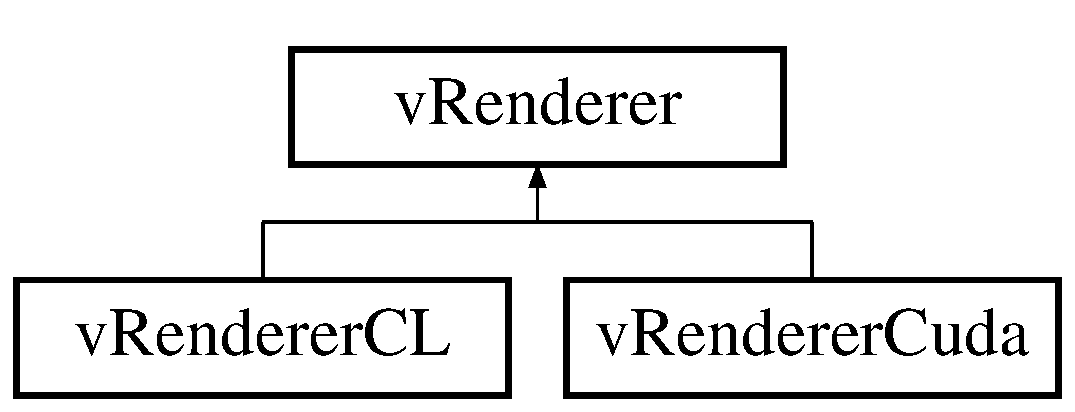
\includegraphics[height=2.000000cm]{classvRenderer}
\end{center}
\end{figure}
\subsection*{Public Member Functions}
\begin{DoxyCompactItemize}
\item 
\hypertarget{classvRenderer_a1ae1d94f9eb933cab90812dd24d5a425}{\hyperlink{classvRenderer_a1ae1d94f9eb933cab90812dd24d5a425}{v\-Renderer} ()}\label{classvRenderer_a1ae1d94f9eb933cab90812dd24d5a425}

\begin{DoxyCompactList}\small\item\em \hyperlink{classvRenderer}{v\-Renderer} Default ctor \end{DoxyCompactList}\item 
\hypertarget{classvRenderer_ad90f4d86e010009e2c7bf2d5ac2cb73e}{virtual \hyperlink{classvRenderer_ad90f4d86e010009e2c7bf2d5ac2cb73e}{$\sim$v\-Renderer} ()}\label{classvRenderer_ad90f4d86e010009e2c7bf2d5ac2cb73e}

\begin{DoxyCompactList}\small\item\em $\sim$v\-Renderer Default virtual dtor \end{DoxyCompactList}\item 
virtual void \hyperlink{classvRenderer_aded5e62557a8e73c5ba81ef2dae422b3}{init} (const unsigned int \&\-\_\-w=0, const unsigned int \&\-\_\-h=0)=0
\begin{DoxyCompactList}\small\item\em init Used to initialise everything that the renderer needs before it can render \end{DoxyCompactList}\item 
virtual void \hyperlink{classvRenderer_adb2aafca5b39b1e6c9b8cf04a7bf4f84}{register\-Texture\-Buffer} (G\-Luint \&\-\_\-texture)=0
\begin{DoxyCompactList}\small\item\em register\-Texture\-Buffer Register the Open\-G\-L texture for Cuda/\-Open\-C\-L interop \end{DoxyCompactList}\item 
virtual void \hyperlink{classvRenderer_a9ffabf6f4fcceac59ad192ef78c4f1b5}{register\-Depth\-Buffer} (G\-Luint \&\-\_\-depth\-Texture)=0
\begin{DoxyCompactList}\small\item\em register\-Depth\-Buffer Register the Open\-G\-L depth texture for Cuda/\-Open\-C\-L interop \end{DoxyCompactList}\item 
\hypertarget{classvRenderer_a2d8fbb867093b06cfa19b099ce3eedb0}{virtual void \hyperlink{classvRenderer_a2d8fbb867093b06cfa19b099ce3eedb0}{render} ()=0}\label{classvRenderer_a2d8fbb867093b06cfa19b099ce3eedb0}

\begin{DoxyCompactList}\small\item\em render Main render function, maps and reserves the needed opengl buffers once available, performs few tracing samples and frees the mapped buffers for drawing \end{DoxyCompactList}\item 
\hypertarget{classvRenderer_a7d9cedd13f2d3e87477a570af14ed7cf}{virtual void \hyperlink{classvRenderer_a7d9cedd13f2d3e87477a570af14ed7cf}{clean\-Up} ()=0}\label{classvRenderer_a7d9cedd13f2d3e87477a570af14ed7cf}

\begin{DoxyCompactList}\small\item\em clean\-Up Cleans the allocated memory and G\-P\-U buffers \end{DoxyCompactList}\item 
\hypertarget{classvRenderer_a19141ca681f34f6ae43919087e6cd83c}{virtual void \hyperlink{classvRenderer_a19141ca681f34f6ae43919087e6cd83c}{update\-Camera} ()=0}\label{classvRenderer_a19141ca681f34f6ae43919087e6cd83c}

\begin{DoxyCompactList}\small\item\em update\-Camera Consumes the updates from the virtual camera and passes the data to the G\-P\-U \end{DoxyCompactList}\item 
virtual void \hyperlink{classvRenderer_aa8e0dd2ed5b56dc3b10a3035d9678557}{init\-Mesh} (const \hyperlink{structvMeshData}{v\-Mesh\-Data} \&\-\_\-sbvh\-Data)=0
\begin{DoxyCompactList}\small\item\em init\-Mesh Takes in 3d mesh data and the \hyperlink{classSBVH}{S\-B\-V\-H} acceleration structure, packs and copies the data to the G\-P\-U \end{DoxyCompactList}\item 
virtual void \hyperlink{classvRenderer_aac0b1a8021d071e0816de34995488f6b}{load\-H\-D\-R} (const Imf\-::\-Rgba $\ast$\-\_\-pixel\-Buffer, const unsigned int \&\-\_\-w, const unsigned int \&\-\_\-h)=0
\begin{DoxyCompactList}\small\item\em load\-H\-D\-R Loads an E\-X\-R pixelbuffer to the G\-P\-U \end{DoxyCompactList}\item 
virtual void \hyperlink{classvRenderer_a904bc18544cfe877fc7e33d12d449c05}{load\-Texture} (const Q\-Image \&\-\_\-texture, const float \&\-\_\-gamma, const unsigned int \&\-\_\-type)=0
\begin{DoxyCompactList}\small\item\em load\-Texture Loads a texture to the G\-P\-U, performs \char`\"{}inverse gamma correction\char`\"{} if needed as gamma correction is applied at the end of each trace step \end{DoxyCompactList}\item 
virtual void \hyperlink{classvRenderer_af2d6b7f027ea76018a83b3c11177c9cf}{use\-B\-R\-D\-F} (const bool \&\-\_\-new\-Val)=0
\begin{DoxyCompactList}\small\item\em use\-B\-R\-D\-F Passes the data to the tracer, whether to use the loaded B\-R\-D\-F data \end{DoxyCompactList}\item 
virtual void \hyperlink{classvRenderer_ac4e01b762661e82813c8909d1c7a47c3}{use\-Example\-Sphere} (const bool \&\-\_\-new\-Val)=0
\begin{DoxyCompactList}\small\item\em use\-Example\-Sphere Passes the info to the tracer, whether to use the example sphere \end{DoxyCompactList}\item 
virtual void \hyperlink{classvRenderer_ad5664d5c12c8869f94f9a65d4d3b2cb9}{use\-Cornell\-Box} (const bool \&\-\_\-new\-Val)=0
\begin{DoxyCompactList}\small\item\em use\-Cornell\-Box Passes the info to the tracer, whether to use the cornell box scene or H\-D\-R\-I environment map \end{DoxyCompactList}\item 
\hypertarget{classvRenderer_a14def36b2a1d0f9c8d346200d81a8e0f}{virtual void \hyperlink{classvRenderer_a14def36b2a1d0f9c8d346200d81a8e0f}{clear\-Buffer} ()=0}\label{classvRenderer_a14def36b2a1d0f9c8d346200d81a8e0f}

\begin{DoxyCompactList}\small\item\em clear\-Buffer Clears the colour buffer, used when something changes in the scene \end{DoxyCompactList}\item 
virtual bool \hyperlink{classvRenderer_a5ef0c07cbcc1d5bbdfd7fe290de700c5}{load\-B\-R\-D\-F} (const float $\ast$\-\_\-brdf)=0
\begin{DoxyCompactList}\small\item\em load\-B\-R\-D\-F Loads the B\-R\-D\-F data to the G\-P\-U \end{DoxyCompactList}\item 
virtual unsigned int \hyperlink{classvRenderer_a623eb6b3f67b6b22137783de6c788e49}{get\-Frame\-Count} () const =0
\begin{DoxyCompactList}\small\item\em get\-Frame\-Count Get the number of frames the current trace has performed \end{DoxyCompactList}\item 
void \hyperlink{classvRenderer_a34b0760641ec58f48eb1029d7f56c82c}{set\-Fresnel\-Coef} (const float \&\-\_\-new\-Val)
\begin{DoxyCompactList}\small\item\em set\-Fresnel\-Coef Set the fresnel coefficient for fresnel-\/like reflections, also clears the colour buffer \end{DoxyCompactList}\item 
void \hyperlink{classvRenderer_a17188eb1567d612d3f27d290e3fd237b}{set\-Fresnel\-Power} (const float \&\-\_\-new\-Val)
\begin{DoxyCompactList}\small\item\em set\-Fresnel\-Power Set the fresnel power for fresnel-\/life reflections, also clears the colour buffer \end{DoxyCompactList}\item 
void \hyperlink{classvRenderer_a329c3c3b1977f7cb6fd465bcd0e13c9f}{set\-Camera} (\hyperlink{classCamera}{Camera} $\ast$\-\_\-cam)
\begin{DoxyCompactList}\small\item\em set\-Camera Initialises the virtual camera for the renderer \end{DoxyCompactList}\end{DoxyCompactItemize}
\subsection*{Protected Attributes}
\begin{DoxyCompactItemize}
\item 
\hypertarget{classvRenderer_adce32b13617ef4ae296b89d622cfab2f}{\hyperlink{classCamera}{Camera} $\ast$ \hyperlink{classvRenderer_adce32b13617ef4ae296b89d622cfab2f}{m\-\_\-virtual\-Camera}}\label{classvRenderer_adce32b13617ef4ae296b89d622cfab2f}

\begin{DoxyCompactList}\small\item\em m\-\_\-virtual\-Camera Pointer to the camera \end{DoxyCompactList}\item 
\hypertarget{classvRenderer_a1aba28d9b3d67626d0fccb0ab02ceda8}{float \hyperlink{classvRenderer_a1aba28d9b3d67626d0fccb0ab02ceda8}{m\-\_\-fresnel\-Coef}}\label{classvRenderer_a1aba28d9b3d67626d0fccb0ab02ceda8}

\begin{DoxyCompactList}\small\item\em m\-\_\-fresnel\-Coef Fresnel coefficient \end{DoxyCompactList}\item 
\hypertarget{classvRenderer_aa0521c8cd17ef469ddccb770b34161dc}{float \hyperlink{classvRenderer_aa0521c8cd17ef469ddccb770b34161dc}{m\-\_\-fresnel\-Pow}}\label{classvRenderer_aa0521c8cd17ef469ddccb770b34161dc}

\begin{DoxyCompactList}\small\item\em m\-\_\-fresnel\-Pow Fresnel power \end{DoxyCompactList}\end{DoxyCompactItemize}


\subsection{Detailed Description}
The \hyperlink{classvRenderer}{v\-Renderer} class Abstract base class for the path tracer. 

\subsection{Member Function Documentation}
\hypertarget{classvRenderer_a623eb6b3f67b6b22137783de6c788e49}{\index{v\-Renderer@{v\-Renderer}!get\-Frame\-Count@{get\-Frame\-Count}}
\index{get\-Frame\-Count@{get\-Frame\-Count}!vRenderer@{v\-Renderer}}
\subsubsection[{get\-Frame\-Count}]{\setlength{\rightskip}{0pt plus 5cm}virtual unsigned int v\-Renderer\-::get\-Frame\-Count (
\begin{DoxyParamCaption}
{}
\end{DoxyParamCaption}
) const\hspace{0.3cm}{\ttfamily [pure virtual]}}}\label{classvRenderer_a623eb6b3f67b6b22137783de6c788e49}


get\-Frame\-Count Get the number of frames the current trace has performed 

\begin{DoxyReturn}{Returns}
The number of frames 
\end{DoxyReturn}


Implemented in \hyperlink{classvRendererCL_a30e02c917778a288dd83a7a29882d030}{v\-Renderer\-C\-L}, and \hyperlink{classvRendererCuda_a59adae8a97ef2a63fc542f64d4686f37}{v\-Renderer\-Cuda}.

\hypertarget{classvRenderer_aded5e62557a8e73c5ba81ef2dae422b3}{\index{v\-Renderer@{v\-Renderer}!init@{init}}
\index{init@{init}!vRenderer@{v\-Renderer}}
\subsubsection[{init}]{\setlength{\rightskip}{0pt plus 5cm}virtual void v\-Renderer\-::init (
\begin{DoxyParamCaption}
\item[{const unsigned int \&}]{\-\_\-w = {\ttfamily 0}, }
\item[{const unsigned int \&}]{\-\_\-h = {\ttfamily 0}}
\end{DoxyParamCaption}
)\hspace{0.3cm}{\ttfamily [pure virtual]}}}\label{classvRenderer_aded5e62557a8e73c5ba81ef2dae422b3}


init Used to initialise everything that the renderer needs before it can render 


\begin{DoxyParams}{Parameters}
{\em \-\_\-w} & Width of the screen \\
\hline
{\em \-\_\-h} & Height of the screen \\
\hline
\end{DoxyParams}


Implemented in \hyperlink{classvRendererCL_a01207b7fea56df11fc2af4cb87cad7e4}{v\-Renderer\-C\-L}, and \hyperlink{classvRendererCuda_a1f6382acd2ad665c724c65a535ed86d1}{v\-Renderer\-Cuda}.

\hypertarget{classvRenderer_aa8e0dd2ed5b56dc3b10a3035d9678557}{\index{v\-Renderer@{v\-Renderer}!init\-Mesh@{init\-Mesh}}
\index{init\-Mesh@{init\-Mesh}!vRenderer@{v\-Renderer}}
\subsubsection[{init\-Mesh}]{\setlength{\rightskip}{0pt plus 5cm}virtual void v\-Renderer\-::init\-Mesh (
\begin{DoxyParamCaption}
\item[{const {\bf v\-Mesh\-Data} \&}]{\-\_\-sbvh\-Data}
\end{DoxyParamCaption}
)\hspace{0.3cm}{\ttfamily [pure virtual]}}}\label{classvRenderer_aa8e0dd2ed5b56dc3b10a3035d9678557}


init\-Mesh Takes in 3d mesh data and the \hyperlink{classSBVH}{S\-B\-V\-H} acceleration structure, packs and copies the data to the G\-P\-U 


\begin{DoxyParams}{Parameters}
{\em \-\_\-sbvh\-Data} & Structure containing the needed data \\
\hline
\end{DoxyParams}


Implemented in \hyperlink{classvRendererCL_a06033a095680d83224fa3d12b703d213}{v\-Renderer\-C\-L}, and \hyperlink{classvRendererCuda_aaad1a6c4a4ada9bbbbce2db3cfb02f32}{v\-Renderer\-Cuda}.

\hypertarget{classvRenderer_a5ef0c07cbcc1d5bbdfd7fe290de700c5}{\index{v\-Renderer@{v\-Renderer}!load\-B\-R\-D\-F@{load\-B\-R\-D\-F}}
\index{load\-B\-R\-D\-F@{load\-B\-R\-D\-F}!vRenderer@{v\-Renderer}}
\subsubsection[{load\-B\-R\-D\-F}]{\setlength{\rightskip}{0pt plus 5cm}virtual bool v\-Renderer\-::load\-B\-R\-D\-F (
\begin{DoxyParamCaption}
\item[{const float $\ast$}]{\-\_\-brdf}
\end{DoxyParamCaption}
)\hspace{0.3cm}{\ttfamily [pure virtual]}}}\label{classvRenderer_a5ef0c07cbcc1d5bbdfd7fe290de700c5}


load\-B\-R\-D\-F Loads the B\-R\-D\-F data to the G\-P\-U 


\begin{DoxyParams}{Parameters}
{\em \-\_\-brdf} & B\-R\-D\-F data read from a binary file \\
\hline
\end{DoxyParams}
\begin{DoxyReturn}{Returns}
True if the data was loaded correctly 
\end{DoxyReturn}


Implemented in \hyperlink{classvRendererCL_a80988c343d250965cc184695fafc7a10}{v\-Renderer\-C\-L}, and \hyperlink{classvRendererCuda_a77eb1673efa671d9a21353fe22f576d7}{v\-Renderer\-Cuda}.

\hypertarget{classvRenderer_aac0b1a8021d071e0816de34995488f6b}{\index{v\-Renderer@{v\-Renderer}!load\-H\-D\-R@{load\-H\-D\-R}}
\index{load\-H\-D\-R@{load\-H\-D\-R}!vRenderer@{v\-Renderer}}
\subsubsection[{load\-H\-D\-R}]{\setlength{\rightskip}{0pt plus 5cm}virtual void v\-Renderer\-::load\-H\-D\-R (
\begin{DoxyParamCaption}
\item[{const Imf\-::\-Rgba $\ast$}]{\-\_\-pixel\-Buffer, }
\item[{const unsigned int \&}]{\-\_\-w, }
\item[{const unsigned int \&}]{\-\_\-h}
\end{DoxyParamCaption}
)\hspace{0.3cm}{\ttfamily [pure virtual]}}}\label{classvRenderer_aac0b1a8021d071e0816de34995488f6b}


load\-H\-D\-R Loads an E\-X\-R pixelbuffer to the G\-P\-U 


\begin{DoxyParams}{Parameters}
{\em \-\_\-pixel\-Buffer} & Loaded pixelbuffer \\
\hline
{\em \-\_\-w} & Width of the H\-D\-R\-I map \\
\hline
{\em \-\_\-h} & Height of the H\-D\-R\-I map \\
\hline
\end{DoxyParams}


Implemented in \hyperlink{classvRendererCL_a4df104a5f4a9e19db7d9c8678ada7cd6}{v\-Renderer\-C\-L}, and \hyperlink{classvRendererCuda_a0994f4f68ad6973f6e80664714eb44e8}{v\-Renderer\-Cuda}.

\hypertarget{classvRenderer_a904bc18544cfe877fc7e33d12d449c05}{\index{v\-Renderer@{v\-Renderer}!load\-Texture@{load\-Texture}}
\index{load\-Texture@{load\-Texture}!vRenderer@{v\-Renderer}}
\subsubsection[{load\-Texture}]{\setlength{\rightskip}{0pt plus 5cm}virtual void v\-Renderer\-::load\-Texture (
\begin{DoxyParamCaption}
\item[{const Q\-Image \&}]{\-\_\-texture, }
\item[{const float \&}]{\-\_\-gamma, }
\item[{const unsigned int \&}]{\-\_\-type}
\end{DoxyParamCaption}
)\hspace{0.3cm}{\ttfamily [pure virtual]}}}\label{classvRenderer_a904bc18544cfe877fc7e33d12d449c05}


load\-Texture Loads a texture to the G\-P\-U, performs \char`\"{}inverse gamma correction\char`\"{} if needed as gamma correction is applied at the end of each trace step 


\begin{DoxyParams}{Parameters}
{\em \-\_\-texture} & Q\-Image to read the texture data from \\
\hline
{\em \-\_\-gamma} & Gamma value of the texture \\
\hline
{\em \-\_\-type} & Type of the texture, 0 = Diffuse, 1 = Normal, 2 = Specular \\
\hline
\end{DoxyParams}


Implemented in \hyperlink{classvRendererCL_aeb2feac32793ba1ab9c74ff3abf9ff78}{v\-Renderer\-C\-L}, and \hyperlink{classvRendererCuda_a1eca8504cfb3287725cef2bbca08180f}{v\-Renderer\-Cuda}.

\hypertarget{classvRenderer_a9ffabf6f4fcceac59ad192ef78c4f1b5}{\index{v\-Renderer@{v\-Renderer}!register\-Depth\-Buffer@{register\-Depth\-Buffer}}
\index{register\-Depth\-Buffer@{register\-Depth\-Buffer}!vRenderer@{v\-Renderer}}
\subsubsection[{register\-Depth\-Buffer}]{\setlength{\rightskip}{0pt plus 5cm}virtual void v\-Renderer\-::register\-Depth\-Buffer (
\begin{DoxyParamCaption}
\item[{G\-Luint \&}]{\-\_\-depth\-Texture}
\end{DoxyParamCaption}
)\hspace{0.3cm}{\ttfamily [pure virtual]}}}\label{classvRenderer_a9ffabf6f4fcceac59ad192ef78c4f1b5}


register\-Depth\-Buffer Register the Open\-G\-L depth texture for Cuda/\-Open\-C\-L interop 


\begin{DoxyParams}{Parameters}
{\em \-\_\-depth\-Texture} & Open\-G\-L depth texture object \\
\hline
\end{DoxyParams}


Implemented in \hyperlink{classvRendererCL_a663d4055fdcc26820c769a3ed11a7cfd}{v\-Renderer\-C\-L}, and \hyperlink{classvRendererCuda_a3374740da969eb673531d99da8a2b2fd}{v\-Renderer\-Cuda}.

\hypertarget{classvRenderer_adb2aafca5b39b1e6c9b8cf04a7bf4f84}{\index{v\-Renderer@{v\-Renderer}!register\-Texture\-Buffer@{register\-Texture\-Buffer}}
\index{register\-Texture\-Buffer@{register\-Texture\-Buffer}!vRenderer@{v\-Renderer}}
\subsubsection[{register\-Texture\-Buffer}]{\setlength{\rightskip}{0pt plus 5cm}virtual void v\-Renderer\-::register\-Texture\-Buffer (
\begin{DoxyParamCaption}
\item[{G\-Luint \&}]{\-\_\-texture}
\end{DoxyParamCaption}
)\hspace{0.3cm}{\ttfamily [pure virtual]}}}\label{classvRenderer_adb2aafca5b39b1e6c9b8cf04a7bf4f84}


register\-Texture\-Buffer Register the Open\-G\-L texture for Cuda/\-Open\-C\-L interop 


\begin{DoxyParams}{Parameters}
{\em \-\_\-texture} & Open\-G\-L texture object \\
\hline
\end{DoxyParams}


Implemented in \hyperlink{classvRendererCL_a124b31960cb2e8cfe821acf888e712a9}{v\-Renderer\-C\-L}, and \hyperlink{classvRendererCuda_aee52063dd808dd194ceb81f54935f099}{v\-Renderer\-Cuda}.

\hypertarget{classvRenderer_a329c3c3b1977f7cb6fd465bcd0e13c9f}{\index{v\-Renderer@{v\-Renderer}!set\-Camera@{set\-Camera}}
\index{set\-Camera@{set\-Camera}!vRenderer@{v\-Renderer}}
\subsubsection[{set\-Camera}]{\setlength{\rightskip}{0pt plus 5cm}void v\-Renderer\-::set\-Camera (
\begin{DoxyParamCaption}
\item[{{\bf Camera} $\ast$}]{\-\_\-cam}
\end{DoxyParamCaption}
)\hspace{0.3cm}{\ttfamily [inline]}}}\label{classvRenderer_a329c3c3b1977f7cb6fd465bcd0e13c9f}


set\-Camera Initialises the virtual camera for the renderer 


\begin{DoxyParams}{Parameters}
{\em \-\_\-cam} & Virtual camera that the renderer will use \\
\hline
\end{DoxyParams}
\hypertarget{classvRenderer_a34b0760641ec58f48eb1029d7f56c82c}{\index{v\-Renderer@{v\-Renderer}!set\-Fresnel\-Coef@{set\-Fresnel\-Coef}}
\index{set\-Fresnel\-Coef@{set\-Fresnel\-Coef}!vRenderer@{v\-Renderer}}
\subsubsection[{set\-Fresnel\-Coef}]{\setlength{\rightskip}{0pt plus 5cm}void v\-Renderer\-::set\-Fresnel\-Coef (
\begin{DoxyParamCaption}
\item[{const float \&}]{\-\_\-new\-Val}
\end{DoxyParamCaption}
)\hspace{0.3cm}{\ttfamily [inline]}}}\label{classvRenderer_a34b0760641ec58f48eb1029d7f56c82c}


set\-Fresnel\-Coef Set the fresnel coefficient for fresnel-\/like reflections, also clears the colour buffer 


\begin{DoxyParams}{Parameters}
{\em \-\_\-new\-Val} & New coefficient \\
\hline
\end{DoxyParams}
\hypertarget{classvRenderer_a17188eb1567d612d3f27d290e3fd237b}{\index{v\-Renderer@{v\-Renderer}!set\-Fresnel\-Power@{set\-Fresnel\-Power}}
\index{set\-Fresnel\-Power@{set\-Fresnel\-Power}!vRenderer@{v\-Renderer}}
\subsubsection[{set\-Fresnel\-Power}]{\setlength{\rightskip}{0pt plus 5cm}void v\-Renderer\-::set\-Fresnel\-Power (
\begin{DoxyParamCaption}
\item[{const float \&}]{\-\_\-new\-Val}
\end{DoxyParamCaption}
)\hspace{0.3cm}{\ttfamily [inline]}}}\label{classvRenderer_a17188eb1567d612d3f27d290e3fd237b}


set\-Fresnel\-Power Set the fresnel power for fresnel-\/life reflections, also clears the colour buffer 


\begin{DoxyParams}{Parameters}
{\em \-\_\-new\-Val} & New power \\
\hline
\end{DoxyParams}
\hypertarget{classvRenderer_af2d6b7f027ea76018a83b3c11177c9cf}{\index{v\-Renderer@{v\-Renderer}!use\-B\-R\-D\-F@{use\-B\-R\-D\-F}}
\index{use\-B\-R\-D\-F@{use\-B\-R\-D\-F}!vRenderer@{v\-Renderer}}
\subsubsection[{use\-B\-R\-D\-F}]{\setlength{\rightskip}{0pt plus 5cm}virtual void v\-Renderer\-::use\-B\-R\-D\-F (
\begin{DoxyParamCaption}
\item[{const bool \&}]{\-\_\-new\-Val}
\end{DoxyParamCaption}
)\hspace{0.3cm}{\ttfamily [pure virtual]}}}\label{classvRenderer_af2d6b7f027ea76018a83b3c11177c9cf}


use\-B\-R\-D\-F Passes the data to the tracer, whether to use the loaded B\-R\-D\-F data 


\begin{DoxyParams}{Parameters}
{\em \-\_\-new\-Val} & Whether to use the loaded B\-R\-D\-F data \\
\hline
\end{DoxyParams}


Implemented in \hyperlink{classvRendererCL_ad08264f1738f5a2effdef21fc3852758}{v\-Renderer\-C\-L}, and \hyperlink{classvRendererCuda_a8bc09351a8cd99d86d36963e430025d7}{v\-Renderer\-Cuda}.

\hypertarget{classvRenderer_ad5664d5c12c8869f94f9a65d4d3b2cb9}{\index{v\-Renderer@{v\-Renderer}!use\-Cornell\-Box@{use\-Cornell\-Box}}
\index{use\-Cornell\-Box@{use\-Cornell\-Box}!vRenderer@{v\-Renderer}}
\subsubsection[{use\-Cornell\-Box}]{\setlength{\rightskip}{0pt plus 5cm}virtual void v\-Renderer\-::use\-Cornell\-Box (
\begin{DoxyParamCaption}
\item[{const bool \&}]{\-\_\-new\-Val}
\end{DoxyParamCaption}
)\hspace{0.3cm}{\ttfamily [pure virtual]}}}\label{classvRenderer_ad5664d5c12c8869f94f9a65d4d3b2cb9}


use\-Cornell\-Box Passes the info to the tracer, whether to use the cornell box scene or H\-D\-R\-I environment map 


\begin{DoxyParams}{Parameters}
{\em \-\_\-new\-Val} & Whether to use cornell box or not \\
\hline
\end{DoxyParams}


Implemented in \hyperlink{classvRendererCL_ae9991460d59a4a86cc19c436a98cd346}{v\-Renderer\-C\-L}, and \hyperlink{classvRendererCuda_a40978e8a1b32dbad5b683b0f097d9c60}{v\-Renderer\-Cuda}.

\hypertarget{classvRenderer_ac4e01b762661e82813c8909d1c7a47c3}{\index{v\-Renderer@{v\-Renderer}!use\-Example\-Sphere@{use\-Example\-Sphere}}
\index{use\-Example\-Sphere@{use\-Example\-Sphere}!vRenderer@{v\-Renderer}}
\subsubsection[{use\-Example\-Sphere}]{\setlength{\rightskip}{0pt plus 5cm}virtual void v\-Renderer\-::use\-Example\-Sphere (
\begin{DoxyParamCaption}
\item[{const bool \&}]{\-\_\-new\-Val}
\end{DoxyParamCaption}
)\hspace{0.3cm}{\ttfamily [pure virtual]}}}\label{classvRenderer_ac4e01b762661e82813c8909d1c7a47c3}


use\-Example\-Sphere Passes the info to the tracer, whether to use the example sphere 


\begin{DoxyParams}{Parameters}
{\em \-\_\-new\-Val} & Whether to use the example sphere \\
\hline
\end{DoxyParams}


Implemented in \hyperlink{classvRendererCL_ace3572b0e58f9ef81ad3853a719d8537}{v\-Renderer\-C\-L}, and \hyperlink{classvRendererCuda_ab552724c473de30893fe9dc21ee2c961}{v\-Renderer\-Cuda}.



The documentation for this class was generated from the following file\-:\begin{DoxyCompactItemize}
\item 
include/\hyperlink{vRenderer_8h}{v\-Renderer.\-h}\end{DoxyCompactItemize}

\hypertarget{classvRendererCL}{\section{v\-Renderer\-C\-L Class Reference}
\label{classvRendererCL}\index{v\-Renderer\-C\-L@{v\-Renderer\-C\-L}}
}


The \hyperlink{classvRendererCL}{v\-Renderer\-C\-L} class Open\-C\-L implementation of the renderer.  




{\ttfamily \#include $<$v\-Renderer\-C\-L.\-h$>$}

Inheritance diagram for v\-Renderer\-C\-L\-:\begin{figure}[H]
\begin{center}
\leavevmode
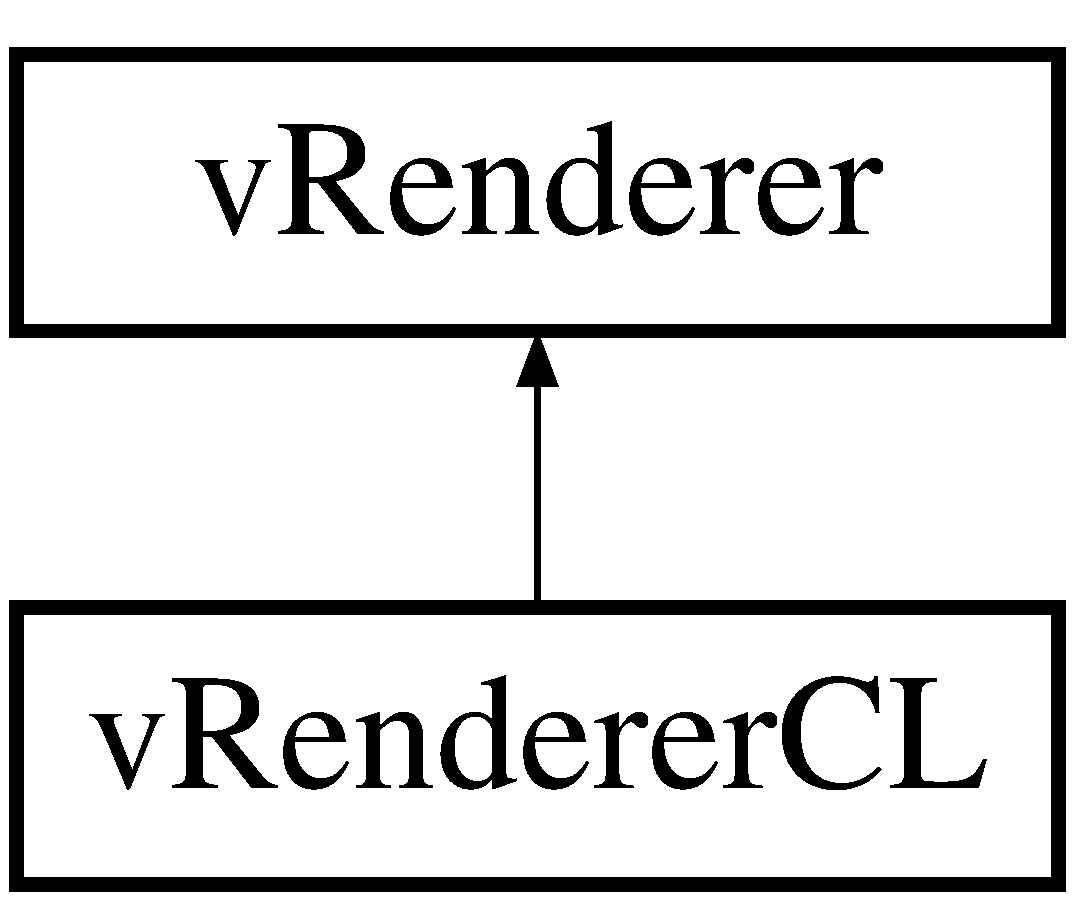
\includegraphics[height=2.000000cm]{classvRendererCL}
\end{center}
\end{figure}
\subsection*{Public Member Functions}
\begin{DoxyCompactItemize}
\item 
\hypertarget{classvRendererCL_a2cc108d7d1b229d5e7ee864e4ba887fb}{\hyperlink{classvRendererCL_a2cc108d7d1b229d5e7ee864e4ba887fb}{v\-Renderer\-C\-L} ()}\label{classvRendererCL_a2cc108d7d1b229d5e7ee864e4ba887fb}

\begin{DoxyCompactList}\small\item\em \hyperlink{classvRendererCL}{v\-Renderer\-C\-L} Default ctor \end{DoxyCompactList}\item 
\hypertarget{classvRendererCL_a30d5cceb0fe2a0592707730a8c61ddf2}{\hyperlink{classvRendererCL_a30d5cceb0fe2a0592707730a8c61ddf2}{$\sim$v\-Renderer\-C\-L} ()}\label{classvRendererCL_a30d5cceb0fe2a0592707730a8c61ddf2}

\begin{DoxyCompactList}\small\item\em $\sim$v\-Renderer\-C\-L Default dtor \end{DoxyCompactList}\item 
void \hyperlink{classvRendererCL_a01207b7fea56df11fc2af4cb87cad7e4}{init} (const unsigned int \&\-\_\-w, const unsigned int \&\-\_\-h) override
\begin{DoxyCompactList}\small\item\em init Creates the Open\-C\-L/\-Open\-G\-L interop context and initialises buffers that are needed at the beginning. Compiles the trace kernels \end{DoxyCompactList}\item 
void \hyperlink{classvRendererCL_a124b31960cb2e8cfe821acf888e712a9}{register\-Texture\-Buffer} (G\-Luint \&\-\_\-texture) override
\begin{DoxyCompactList}\small\item\em register\-Texture\-Buffer Register the Open\-G\-L texture for Open\-C\-L interop \end{DoxyCompactList}\item 
void \hyperlink{classvRendererCL_a663d4055fdcc26820c769a3ed11a7cfd}{register\-Depth\-Buffer} (G\-Luint \&\-\_\-depth\-Texture) override
\begin{DoxyCompactList}\small\item\em register\-Depth\-Buffer Register the Open\-G\-L depth texture for Open\-C\-L interop, not implemented for now \end{DoxyCompactList}\item 
\hypertarget{classvRendererCL_a7bc6f37f611bc3d356ca25c6e2cd200b}{void \hyperlink{classvRendererCL_a7bc6f37f611bc3d356ca25c6e2cd200b}{render} () override}\label{classvRendererCL_a7bc6f37f611bc3d356ca25c6e2cd200b}

\begin{DoxyCompactList}\small\item\em render Render function, passes the G\-P\-U buffers and arguments to the kernel and reserves the needed Open\-G\-L resources and frees them once done \end{DoxyCompactList}\item 
\hypertarget{classvRendererCL_a8b72cc2f7d637774e285105437af33d1}{void \hyperlink{classvRendererCL_a8b72cc2f7d637774e285105437af33d1}{clean\-Up} () override}\label{classvRendererCL_a8b72cc2f7d637774e285105437af33d1}

\begin{DoxyCompactList}\small\item\em clean\-Up Clears and frees the allocated memory and buffers \end{DoxyCompactList}\item 
\hypertarget{classvRendererCL_a9f8885e7a31fb62fdd32304ac422b56b}{void \hyperlink{classvRendererCL_a9f8885e7a31fb62fdd32304ac422b56b}{update\-Camera} () override}\label{classvRendererCL_a9f8885e7a31fb62fdd32304ac422b56b}

\begin{DoxyCompactList}\small\item\em update\-Camera Consumes the updates from the virtual camera and passes the data to the G\-P\-U \end{DoxyCompactList}\item 
void \hyperlink{classvRendererCL_a06033a095680d83224fa3d12b703d213}{init\-Mesh} (const \hyperlink{structvMeshData}{v\-Mesh\-Data} \&\-\_\-mesh\-Data) override
\begin{DoxyCompactList}\small\item\em init\-Mesh Takes in 3d mesh data and the \hyperlink{classSBVH}{S\-B\-V\-H} acceleration structure, packs and copies the data to the G\-P\-U \end{DoxyCompactList}\item 
void \hyperlink{classvRendererCL_a4df104a5f4a9e19db7d9c8678ada7cd6}{load\-H\-D\-R} (const Imf\-::\-Rgba $\ast$\-\_\-colours, const unsigned int \&\-\_\-w, const unsigned int \&\-\_\-h) override
\begin{DoxyCompactList}\small\item\em load\-H\-D\-R Loads an E\-X\-R pixelbuffer to the G\-P\-U \end{DoxyCompactList}\item 
void \hyperlink{classvRendererCL_aeb2feac32793ba1ab9c74ff3abf9ff78}{load\-Texture} (const Q\-Image \&\-\_\-texture, const float \&\-\_\-gamma, const unsigned int \&\-\_\-type) override
\begin{DoxyCompactList}\small\item\em load\-Texture Loads a texture to the G\-P\-U, performs \char`\"{}inverse gamma correction\char`\"{} if needed as gamma correction is applied at the end of each trace step \end{DoxyCompactList}\item 
void \hyperlink{classvRendererCL_ad08264f1738f5a2effdef21fc3852758}{use\-B\-R\-D\-F} (const bool \&\-\_\-new\-Val) override
\begin{DoxyCompactList}\small\item\em use\-B\-R\-D\-F Passes the data to the tracer, whether to use the loaded B\-R\-D\-F data \end{DoxyCompactList}\item 
void \hyperlink{classvRendererCL_ace3572b0e58f9ef81ad3853a719d8537}{use\-Example\-Sphere} (const bool \&\-\_\-new\-Val) override
\begin{DoxyCompactList}\small\item\em use\-Example\-Sphere Passes the info to the tracer, whether to use the example sphere \end{DoxyCompactList}\item 
void \hyperlink{classvRendererCL_ae9991460d59a4a86cc19c436a98cd346}{use\-Cornell\-Box} (const bool \&\-\_\-new\-Val) override
\begin{DoxyCompactList}\small\item\em use\-Cornell\-Box Passes the info to the tracer, whether to use the cornell box scene or H\-D\-R\-I environment map \end{DoxyCompactList}\item 
\hypertarget{classvRendererCL_aeee2cef9e03af6095ea0b8237d2ab184}{void \hyperlink{classvRendererCL_aeee2cef9e03af6095ea0b8237d2ab184}{clear\-Buffer} () override}\label{classvRendererCL_aeee2cef9e03af6095ea0b8237d2ab184}

\begin{DoxyCompactList}\small\item\em clear\-Buffer Clears the colour buffer, used when something changes in the scene \end{DoxyCompactList}\item 
bool \hyperlink{classvRendererCL_a80988c343d250965cc184695fafc7a10}{load\-B\-R\-D\-F} (const float $\ast$\-\_\-brdf) override
\begin{DoxyCompactList}\small\item\em load\-B\-R\-D\-F Loads the B\-R\-D\-F data to the G\-P\-U \end{DoxyCompactList}\item 
unsigned int \hyperlink{classvRendererCL_a30e02c917778a288dd83a7a29882d030}{get\-Frame\-Count} () const override
\begin{DoxyCompactList}\small\item\em get\-Frame\-Count Get the number of frames the current trace has performed \end{DoxyCompactList}\end{DoxyCompactItemize}
\subsection*{Additional Inherited Members}


\subsection{Detailed Description}
The \hyperlink{classvRendererCL}{v\-Renderer\-C\-L} class Open\-C\-L implementation of the renderer. 

\subsection{Member Function Documentation}
\hypertarget{classvRendererCL_a30e02c917778a288dd83a7a29882d030}{\index{v\-Renderer\-C\-L@{v\-Renderer\-C\-L}!get\-Frame\-Count@{get\-Frame\-Count}}
\index{get\-Frame\-Count@{get\-Frame\-Count}!vRendererCL@{v\-Renderer\-C\-L}}
\subsubsection[{get\-Frame\-Count}]{\setlength{\rightskip}{0pt plus 5cm}unsigned int v\-Renderer\-C\-L\-::get\-Frame\-Count (
\begin{DoxyParamCaption}
{}
\end{DoxyParamCaption}
) const\hspace{0.3cm}{\ttfamily [inline]}, {\ttfamily [override]}, {\ttfamily [virtual]}}}\label{classvRendererCL_a30e02c917778a288dd83a7a29882d030}


get\-Frame\-Count Get the number of frames the current trace has performed 

\begin{DoxyReturn}{Returns}
The number of frames 
\end{DoxyReturn}


Implements \hyperlink{classvRenderer_a623eb6b3f67b6b22137783de6c788e49}{v\-Renderer}.

\hypertarget{classvRendererCL_a01207b7fea56df11fc2af4cb87cad7e4}{\index{v\-Renderer\-C\-L@{v\-Renderer\-C\-L}!init@{init}}
\index{init@{init}!vRendererCL@{v\-Renderer\-C\-L}}
\subsubsection[{init}]{\setlength{\rightskip}{0pt plus 5cm}void v\-Renderer\-C\-L\-::init (
\begin{DoxyParamCaption}
\item[{const unsigned int \&}]{\-\_\-w, }
\item[{const unsigned int \&}]{\-\_\-h}
\end{DoxyParamCaption}
)\hspace{0.3cm}{\ttfamily [override]}, {\ttfamily [virtual]}}}\label{classvRendererCL_a01207b7fea56df11fc2af4cb87cad7e4}


init Creates the Open\-C\-L/\-Open\-G\-L interop context and initialises buffers that are needed at the beginning. Compiles the trace kernels 


\begin{DoxyParams}{Parameters}
{\em \-\_\-w} & Width of the screen \\
\hline
{\em \-\_\-h} & Height of the screen \\
\hline
\end{DoxyParams}
Get and create Open\-C\-L/\-Open\-G\-L interop context

Implements \hyperlink{classvRenderer_aded5e62557a8e73c5ba81ef2dae422b3}{v\-Renderer}.

\hypertarget{classvRendererCL_a06033a095680d83224fa3d12b703d213}{\index{v\-Renderer\-C\-L@{v\-Renderer\-C\-L}!init\-Mesh@{init\-Mesh}}
\index{init\-Mesh@{init\-Mesh}!vRendererCL@{v\-Renderer\-C\-L}}
\subsubsection[{init\-Mesh}]{\setlength{\rightskip}{0pt plus 5cm}void v\-Renderer\-C\-L\-::init\-Mesh (
\begin{DoxyParamCaption}
\item[{const {\bf v\-Mesh\-Data} \&}]{\-\_\-mesh\-Data}
\end{DoxyParamCaption}
)\hspace{0.3cm}{\ttfamily [override]}, {\ttfamily [virtual]}}}\label{classvRendererCL_a06033a095680d83224fa3d12b703d213}


init\-Mesh Takes in 3d mesh data and the \hyperlink{classSBVH}{S\-B\-V\-H} acceleration structure, packs and copies the data to the G\-P\-U 


\begin{DoxyParams}{Parameters}
{\em \-\_\-sbvh\-Data} & Structure containing the needed data \\
\hline
\end{DoxyParams}


Implements \hyperlink{classvRenderer_aa8e0dd2ed5b56dc3b10a3035d9678557}{v\-Renderer}.

\hypertarget{classvRendererCL_a80988c343d250965cc184695fafc7a10}{\index{v\-Renderer\-C\-L@{v\-Renderer\-C\-L}!load\-B\-R\-D\-F@{load\-B\-R\-D\-F}}
\index{load\-B\-R\-D\-F@{load\-B\-R\-D\-F}!vRendererCL@{v\-Renderer\-C\-L}}
\subsubsection[{load\-B\-R\-D\-F}]{\setlength{\rightskip}{0pt plus 5cm}bool v\-Renderer\-C\-L\-::load\-B\-R\-D\-F (
\begin{DoxyParamCaption}
\item[{const float $\ast$}]{\-\_\-brdf}
\end{DoxyParamCaption}
)\hspace{0.3cm}{\ttfamily [override]}, {\ttfamily [virtual]}}}\label{classvRendererCL_a80988c343d250965cc184695fafc7a10}


load\-B\-R\-D\-F Loads the B\-R\-D\-F data to the G\-P\-U 


\begin{DoxyParams}{Parameters}
{\em \-\_\-brdf} & B\-R\-D\-F data read from a binary file \\
\hline
\end{DoxyParams}
\begin{DoxyReturn}{Returns}
True if the data was loaded correctly 
\end{DoxyReturn}


Implements \hyperlink{classvRenderer_a5ef0c07cbcc1d5bbdfd7fe290de700c5}{v\-Renderer}.

\hypertarget{classvRendererCL_a4df104a5f4a9e19db7d9c8678ada7cd6}{\index{v\-Renderer\-C\-L@{v\-Renderer\-C\-L}!load\-H\-D\-R@{load\-H\-D\-R}}
\index{load\-H\-D\-R@{load\-H\-D\-R}!vRendererCL@{v\-Renderer\-C\-L}}
\subsubsection[{load\-H\-D\-R}]{\setlength{\rightskip}{0pt plus 5cm}void v\-Renderer\-C\-L\-::load\-H\-D\-R (
\begin{DoxyParamCaption}
\item[{const Imf\-::\-Rgba $\ast$}]{\-\_\-colours, }
\item[{const unsigned int \&}]{\-\_\-w, }
\item[{const unsigned int \&}]{\-\_\-h}
\end{DoxyParamCaption}
)\hspace{0.3cm}{\ttfamily [override]}, {\ttfamily [virtual]}}}\label{classvRendererCL_a4df104a5f4a9e19db7d9c8678ada7cd6}


load\-H\-D\-R Loads an E\-X\-R pixelbuffer to the G\-P\-U 


\begin{DoxyParams}{Parameters}
{\em \-\_\-pixel\-Buffer} & Loaded pixelbuffer \\
\hline
{\em \-\_\-w} & Width of the H\-D\-R\-I map \\
\hline
{\em \-\_\-h} & Height of the H\-D\-R\-I map \\
\hline
\end{DoxyParams}


Implements \hyperlink{classvRenderer_aac0b1a8021d071e0816de34995488f6b}{v\-Renderer}.

\hypertarget{classvRendererCL_aeb2feac32793ba1ab9c74ff3abf9ff78}{\index{v\-Renderer\-C\-L@{v\-Renderer\-C\-L}!load\-Texture@{load\-Texture}}
\index{load\-Texture@{load\-Texture}!vRendererCL@{v\-Renderer\-C\-L}}
\subsubsection[{load\-Texture}]{\setlength{\rightskip}{0pt plus 5cm}void v\-Renderer\-C\-L\-::load\-Texture (
\begin{DoxyParamCaption}
\item[{const Q\-Image \&}]{\-\_\-texture, }
\item[{const float \&}]{\-\_\-gamma, }
\item[{const unsigned int \&}]{\-\_\-type}
\end{DoxyParamCaption}
)\hspace{0.3cm}{\ttfamily [override]}, {\ttfamily [virtual]}}}\label{classvRendererCL_aeb2feac32793ba1ab9c74ff3abf9ff78}


load\-Texture Loads a texture to the G\-P\-U, performs \char`\"{}inverse gamma correction\char`\"{} if needed as gamma correction is applied at the end of each trace step 


\begin{DoxyParams}{Parameters}
{\em \-\_\-texture} & Q\-Image to read the texture data from \\
\hline
{\em \-\_\-gamma} & Gamma value of the texture \\
\hline
{\em \-\_\-type} & Type of the texture, 0 = Diffuse, 1 = Normal, 2 = Specular \\
\hline
\end{DoxyParams}


Implements \hyperlink{classvRenderer_a904bc18544cfe877fc7e33d12d449c05}{v\-Renderer}.

\hypertarget{classvRendererCL_a663d4055fdcc26820c769a3ed11a7cfd}{\index{v\-Renderer\-C\-L@{v\-Renderer\-C\-L}!register\-Depth\-Buffer@{register\-Depth\-Buffer}}
\index{register\-Depth\-Buffer@{register\-Depth\-Buffer}!vRendererCL@{v\-Renderer\-C\-L}}
\subsubsection[{register\-Depth\-Buffer}]{\setlength{\rightskip}{0pt plus 5cm}void v\-Renderer\-C\-L\-::register\-Depth\-Buffer (
\begin{DoxyParamCaption}
\item[{G\-Luint \&}]{\-\_\-depth\-Texture}
\end{DoxyParamCaption}
)\hspace{0.3cm}{\ttfamily [override]}, {\ttfamily [virtual]}}}\label{classvRendererCL_a663d4055fdcc26820c769a3ed11a7cfd}


register\-Depth\-Buffer Register the Open\-G\-L depth texture for Open\-C\-L interop, not implemented for now 


\begin{DoxyParams}{Parameters}
{\em \-\_\-depth\-Texture} & Open\-G\-L depth texture object \\
\hline
\end{DoxyParams}


Implements \hyperlink{classvRenderer_a9ffabf6f4fcceac59ad192ef78c4f1b5}{v\-Renderer}.

\hypertarget{classvRendererCL_a124b31960cb2e8cfe821acf888e712a9}{\index{v\-Renderer\-C\-L@{v\-Renderer\-C\-L}!register\-Texture\-Buffer@{register\-Texture\-Buffer}}
\index{register\-Texture\-Buffer@{register\-Texture\-Buffer}!vRendererCL@{v\-Renderer\-C\-L}}
\subsubsection[{register\-Texture\-Buffer}]{\setlength{\rightskip}{0pt plus 5cm}void v\-Renderer\-C\-L\-::register\-Texture\-Buffer (
\begin{DoxyParamCaption}
\item[{G\-Luint \&}]{\-\_\-texture}
\end{DoxyParamCaption}
)\hspace{0.3cm}{\ttfamily [override]}, {\ttfamily [virtual]}}}\label{classvRendererCL_a124b31960cb2e8cfe821acf888e712a9}


register\-Texture\-Buffer Register the Open\-G\-L texture for Open\-C\-L interop 


\begin{DoxyParams}{Parameters}
{\em \-\_\-texture} & Open\-G\-L texture object \\
\hline
\end{DoxyParams}


Implements \hyperlink{classvRenderer_adb2aafca5b39b1e6c9b8cf04a7bf4f84}{v\-Renderer}.

\hypertarget{classvRendererCL_ad08264f1738f5a2effdef21fc3852758}{\index{v\-Renderer\-C\-L@{v\-Renderer\-C\-L}!use\-B\-R\-D\-F@{use\-B\-R\-D\-F}}
\index{use\-B\-R\-D\-F@{use\-B\-R\-D\-F}!vRendererCL@{v\-Renderer\-C\-L}}
\subsubsection[{use\-B\-R\-D\-F}]{\setlength{\rightskip}{0pt plus 5cm}void v\-Renderer\-C\-L\-::use\-B\-R\-D\-F (
\begin{DoxyParamCaption}
\item[{const bool \&}]{\-\_\-new\-Val}
\end{DoxyParamCaption}
)\hspace{0.3cm}{\ttfamily [override]}, {\ttfamily [virtual]}}}\label{classvRendererCL_ad08264f1738f5a2effdef21fc3852758}


use\-B\-R\-D\-F Passes the data to the tracer, whether to use the loaded B\-R\-D\-F data 


\begin{DoxyParams}{Parameters}
{\em \-\_\-new\-Val} & Whether to use the loaded B\-R\-D\-F data \\
\hline
\end{DoxyParams}


Implements \hyperlink{classvRenderer_af2d6b7f027ea76018a83b3c11177c9cf}{v\-Renderer}.

\hypertarget{classvRendererCL_ae9991460d59a4a86cc19c436a98cd346}{\index{v\-Renderer\-C\-L@{v\-Renderer\-C\-L}!use\-Cornell\-Box@{use\-Cornell\-Box}}
\index{use\-Cornell\-Box@{use\-Cornell\-Box}!vRendererCL@{v\-Renderer\-C\-L}}
\subsubsection[{use\-Cornell\-Box}]{\setlength{\rightskip}{0pt plus 5cm}void v\-Renderer\-C\-L\-::use\-Cornell\-Box (
\begin{DoxyParamCaption}
\item[{const bool \&}]{\-\_\-new\-Val}
\end{DoxyParamCaption}
)\hspace{0.3cm}{\ttfamily [override]}, {\ttfamily [virtual]}}}\label{classvRendererCL_ae9991460d59a4a86cc19c436a98cd346}


use\-Cornell\-Box Passes the info to the tracer, whether to use the cornell box scene or H\-D\-R\-I environment map 


\begin{DoxyParams}{Parameters}
{\em \-\_\-new\-Val} & Whether to use cornell box or not \\
\hline
\end{DoxyParams}


Implements \hyperlink{classvRenderer_ad5664d5c12c8869f94f9a65d4d3b2cb9}{v\-Renderer}.

\hypertarget{classvRendererCL_ace3572b0e58f9ef81ad3853a719d8537}{\index{v\-Renderer\-C\-L@{v\-Renderer\-C\-L}!use\-Example\-Sphere@{use\-Example\-Sphere}}
\index{use\-Example\-Sphere@{use\-Example\-Sphere}!vRendererCL@{v\-Renderer\-C\-L}}
\subsubsection[{use\-Example\-Sphere}]{\setlength{\rightskip}{0pt plus 5cm}void v\-Renderer\-C\-L\-::use\-Example\-Sphere (
\begin{DoxyParamCaption}
\item[{const bool \&}]{\-\_\-new\-Val}
\end{DoxyParamCaption}
)\hspace{0.3cm}{\ttfamily [override]}, {\ttfamily [virtual]}}}\label{classvRendererCL_ace3572b0e58f9ef81ad3853a719d8537}


use\-Example\-Sphere Passes the info to the tracer, whether to use the example sphere 


\begin{DoxyParams}{Parameters}
{\em \-\_\-new\-Val} & Whether to use the example sphere \\
\hline
\end{DoxyParams}


Implements \hyperlink{classvRenderer_ac4e01b762661e82813c8909d1c7a47c3}{v\-Renderer}.



The documentation for this class was generated from the following files\-:\begin{DoxyCompactItemize}
\item 
include/\hyperlink{vRendererCL_8h}{v\-Renderer\-C\-L.\-h}\item 
src/\hyperlink{vRendererCL_8cpp}{v\-Renderer\-C\-L.\-cpp}\end{DoxyCompactItemize}

\hypertarget{classvRendererCuda}{\section{v\-Renderer\-Cuda Class Reference}
\label{classvRendererCuda}\index{v\-Renderer\-Cuda@{v\-Renderer\-Cuda}}
}


The \hyperlink{classvRendererCuda}{v\-Renderer\-Cuda} class Cuda implementation of the renderer.  




{\ttfamily \#include $<$v\-Renderer\-Cuda.\-h$>$}

Inheritance diagram for v\-Renderer\-Cuda\-:\begin{figure}[H]
\begin{center}
\leavevmode
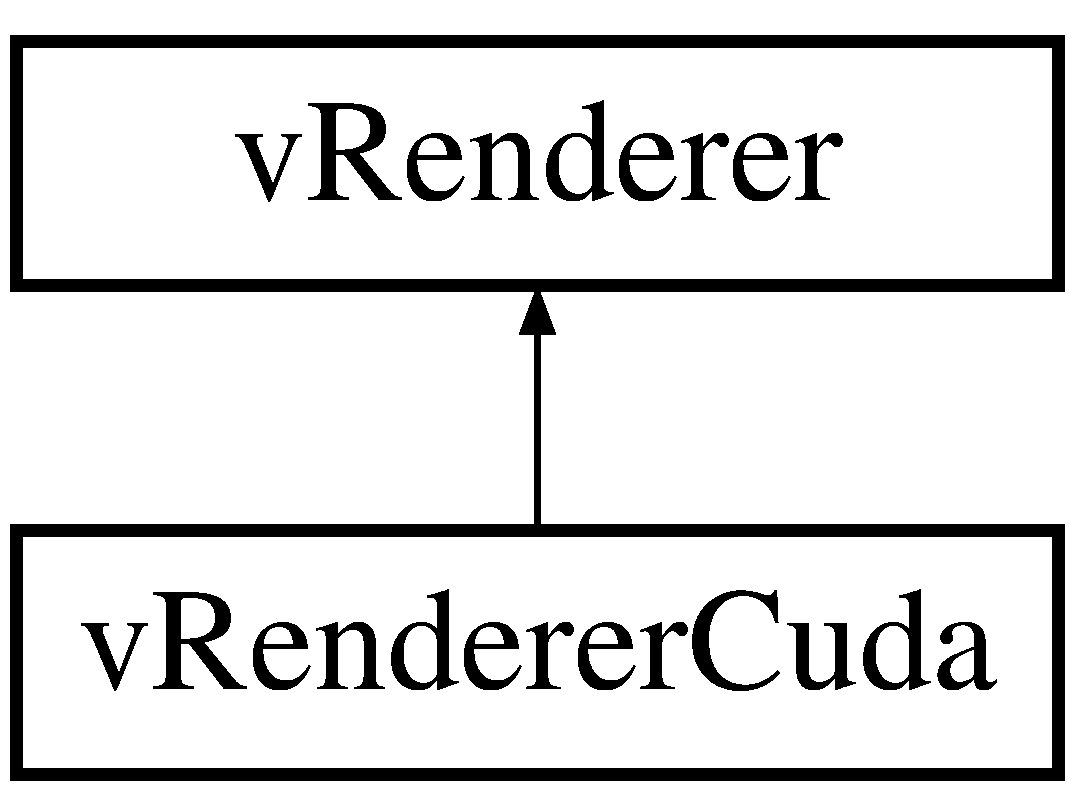
\includegraphics[height=2.000000cm]{classvRendererCuda}
\end{center}
\end{figure}
\subsection*{Public Member Functions}
\begin{DoxyCompactItemize}
\item 
\hypertarget{classvRendererCuda_ab221aa7875d1a7ec689e64e771bbde4c}{\hyperlink{classvRendererCuda_ab221aa7875d1a7ec689e64e771bbde4c}{v\-Renderer\-Cuda} ()}\label{classvRendererCuda_ab221aa7875d1a7ec689e64e771bbde4c}

\begin{DoxyCompactList}\small\item\em \hyperlink{classvRendererCuda}{v\-Renderer\-Cuda} Default ctor \end{DoxyCompactList}\item 
\hypertarget{classvRendererCuda_a16481f8b297fbe0e74dfb6e93b6b4047}{\hyperlink{classvRendererCuda_a16481f8b297fbe0e74dfb6e93b6b4047}{$\sim$v\-Renderer\-Cuda} ()}\label{classvRendererCuda_a16481f8b297fbe0e74dfb6e93b6b4047}

\begin{DoxyCompactList}\small\item\em $\sim$v\-Renderer\-Cuda Default dtor, calls the cleanup routine \end{DoxyCompactList}\item 
void \hyperlink{classvRendererCuda_a1f6382acd2ad665c724c65a535ed86d1}{init} (const unsigned int \&\-\_\-w, const unsigned int \&\-\_\-h) override
\begin{DoxyCompactList}\small\item\em init \end{DoxyCompactList}\item 
void \hyperlink{classvRendererCuda_aee52063dd808dd194ceb81f54935f099}{register\-Texture\-Buffer} (G\-Luint \&\-\_\-texture) override
\begin{DoxyCompactList}\small\item\em register\-Texture\-Buffer Register the Open\-G\-L texture for Cuda interop \end{DoxyCompactList}\item 
void \hyperlink{classvRendererCuda_a3374740da969eb673531d99da8a2b2fd}{register\-Depth\-Buffer} (G\-Luint \&\-\_\-depth\-Texture) override
\begin{DoxyCompactList}\small\item\em register\-Depth\-Buffer Register the Open\-G\-L depth texture for Cuda interop \end{DoxyCompactList}\item 
\hypertarget{classvRendererCuda_a8a4f054aadca6b47f885d92f3d8460c3}{void \hyperlink{classvRendererCuda_a8a4f054aadca6b47f885d92f3d8460c3}{render} () override}\label{classvRendererCuda_a8a4f054aadca6b47f885d92f3d8460c3}

\begin{DoxyCompactList}\small\item\em render Render function, passes the G\-P\-U buffers and arguments to the kernel and reserves the needed Open\-G\-L resources and frees them once done \end{DoxyCompactList}\item 
\hypertarget{classvRendererCuda_afa14d96fa05a162a51f8d644cdd1ed1f}{void \hyperlink{classvRendererCuda_afa14d96fa05a162a51f8d644cdd1ed1f}{clean\-Up} () override}\label{classvRendererCuda_afa14d96fa05a162a51f8d644cdd1ed1f}

\begin{DoxyCompactList}\small\item\em clean\-Up Clears and frees the allocated memory and buffers \end{DoxyCompactList}\item 
\hypertarget{classvRendererCuda_a07f5dc38a31d3d165192e85543fb1781}{void \hyperlink{classvRendererCuda_a07f5dc38a31d3d165192e85543fb1781}{update\-Camera} () override}\label{classvRendererCuda_a07f5dc38a31d3d165192e85543fb1781}

\begin{DoxyCompactList}\small\item\em update\-Camera Consumes the updates from the virtual camera and passes the data to the G\-P\-U \end{DoxyCompactList}\item 
void \hyperlink{classvRendererCuda_aaad1a6c4a4ada9bbbbce2db3cfb02f32}{init\-Mesh} (const \hyperlink{structvMeshData}{v\-Mesh\-Data} \&\-\_\-mesh\-Data) override
\begin{DoxyCompactList}\small\item\em init\-Mesh Takes in 3d mesh data and the \hyperlink{classSBVH}{S\-B\-V\-H} acceleration structure, packs and copies the data to the G\-P\-U \end{DoxyCompactList}\item 
void \hyperlink{classvRendererCuda_a0994f4f68ad6973f6e80664714eb44e8}{load\-H\-D\-R} (const Imf\-::\-Rgba $\ast$\-\_\-colours, const unsigned int \&\-\_\-w, const unsigned int \&\-\_\-h) override
\begin{DoxyCompactList}\small\item\em load\-H\-D\-R Loads an E\-X\-R pixelbuffer to the G\-P\-U \end{DoxyCompactList}\item 
void \hyperlink{classvRendererCuda_a1eca8504cfb3287725cef2bbca08180f}{load\-Texture} (const Q\-Image \&\-\_\-texture, const float \&\-\_\-gamma, const unsigned int \&\-\_\-type) override
\begin{DoxyCompactList}\small\item\em load\-Texture Loads a texture to the G\-P\-U, performs \char`\"{}inverse gamma correction\char`\"{} if needed as gamma correction is applied at the end of each trace step \end{DoxyCompactList}\item 
void \hyperlink{classvRendererCuda_a8bc09351a8cd99d86d36963e430025d7}{use\-B\-R\-D\-F} (const bool \&\-\_\-new\-Val) override
\begin{DoxyCompactList}\small\item\em use\-B\-R\-D\-F Passes the data to the tracer, whether to use the loaded B\-R\-D\-F data \end{DoxyCompactList}\item 
void \hyperlink{classvRendererCuda_ab552724c473de30893fe9dc21ee2c961}{use\-Example\-Sphere} (const bool \&\-\_\-new\-Val) override
\begin{DoxyCompactList}\small\item\em use\-Example\-Sphere Passes the info to the tracer, whether to use the example sphere \end{DoxyCompactList}\item 
void \hyperlink{classvRendererCuda_a40978e8a1b32dbad5b683b0f097d9c60}{use\-Cornell\-Box} (const bool \&\-\_\-new\-Val) override
\begin{DoxyCompactList}\small\item\em use\-Cornell\-Box Passes the info to the tracer, whether to use the cornell box scene or H\-D\-R\-I environment map \end{DoxyCompactList}\item 
\hypertarget{classvRendererCuda_a1fd902cd1f41af0baca67bb50b88226c}{void \hyperlink{classvRendererCuda_a1fd902cd1f41af0baca67bb50b88226c}{clear\-Buffer} () override}\label{classvRendererCuda_a1fd902cd1f41af0baca67bb50b88226c}

\begin{DoxyCompactList}\small\item\em clear\-Buffer Clears the colour buffer, used when something changes in the scene \end{DoxyCompactList}\item 
bool \hyperlink{classvRendererCuda_a77eb1673efa671d9a21353fe22f576d7}{load\-B\-R\-D\-F} (const float $\ast$\-\_\-brdf) override
\begin{DoxyCompactList}\small\item\em load\-B\-R\-D\-F Loads the B\-R\-D\-F data to the G\-P\-U \end{DoxyCompactList}\item 
unsigned int \hyperlink{classvRendererCuda_a59adae8a97ef2a63fc542f64d4686f37}{get\-Frame\-Count} () const override
\begin{DoxyCompactList}\small\item\em get\-Frame\-Count Get the number of frames the current trace has performed \end{DoxyCompactList}\end{DoxyCompactItemize}
\subsection*{Additional Inherited Members}


\subsection{Detailed Description}
The \hyperlink{classvRendererCuda}{v\-Renderer\-Cuda} class Cuda implementation of the renderer. 

\subsection{Member Function Documentation}
\hypertarget{classvRendererCuda_a59adae8a97ef2a63fc542f64d4686f37}{\index{v\-Renderer\-Cuda@{v\-Renderer\-Cuda}!get\-Frame\-Count@{get\-Frame\-Count}}
\index{get\-Frame\-Count@{get\-Frame\-Count}!vRendererCuda@{v\-Renderer\-Cuda}}
\subsubsection[{get\-Frame\-Count}]{\setlength{\rightskip}{0pt plus 5cm}unsigned int v\-Renderer\-Cuda\-::get\-Frame\-Count (
\begin{DoxyParamCaption}
{}
\end{DoxyParamCaption}
) const\hspace{0.3cm}{\ttfamily [inline]}, {\ttfamily [override]}, {\ttfamily [virtual]}}}\label{classvRendererCuda_a59adae8a97ef2a63fc542f64d4686f37}


get\-Frame\-Count Get the number of frames the current trace has performed 

\begin{DoxyReturn}{Returns}
The number of frames 
\end{DoxyReturn}


Implements \hyperlink{classvRenderer_a623eb6b3f67b6b22137783de6c788e49}{v\-Renderer}.

\hypertarget{classvRendererCuda_a1f6382acd2ad665c724c65a535ed86d1}{\index{v\-Renderer\-Cuda@{v\-Renderer\-Cuda}!init@{init}}
\index{init@{init}!vRendererCuda@{v\-Renderer\-Cuda}}
\subsubsection[{init}]{\setlength{\rightskip}{0pt plus 5cm}void v\-Renderer\-Cuda\-::init (
\begin{DoxyParamCaption}
\item[{const unsigned int \&}]{\-\_\-w, }
\item[{const unsigned int \&}]{\-\_\-h}
\end{DoxyParamCaption}
)\hspace{0.3cm}{\ttfamily [override]}, {\ttfamily [virtual]}}}\label{classvRendererCuda_a1f6382acd2ad665c724c65a535ed86d1}


init 


\begin{DoxyParams}{Parameters}
{\em \-\_\-w} & \\
\hline
{\em \-\_\-h} & \\
\hline
\end{DoxyParams}


Implements \hyperlink{classvRenderer_aded5e62557a8e73c5ba81ef2dae422b3}{v\-Renderer}.

\hypertarget{classvRendererCuda_aaad1a6c4a4ada9bbbbce2db3cfb02f32}{\index{v\-Renderer\-Cuda@{v\-Renderer\-Cuda}!init\-Mesh@{init\-Mesh}}
\index{init\-Mesh@{init\-Mesh}!vRendererCuda@{v\-Renderer\-Cuda}}
\subsubsection[{init\-Mesh}]{\setlength{\rightskip}{0pt plus 5cm}void v\-Renderer\-Cuda\-::init\-Mesh (
\begin{DoxyParamCaption}
\item[{const {\bf v\-Mesh\-Data} \&}]{\-\_\-mesh\-Data}
\end{DoxyParamCaption}
)\hspace{0.3cm}{\ttfamily [override]}, {\ttfamily [virtual]}}}\label{classvRendererCuda_aaad1a6c4a4ada9bbbbce2db3cfb02f32}


init\-Mesh Takes in 3d mesh data and the \hyperlink{classSBVH}{S\-B\-V\-H} acceleration structure, packs and copies the data to the G\-P\-U 


\begin{DoxyParams}{Parameters}
{\em \-\_\-sbvh\-Data} & Structure containing the needed data \\
\hline
\end{DoxyParams}


Implements \hyperlink{classvRenderer_aa8e0dd2ed5b56dc3b10a3035d9678557}{v\-Renderer}.

\hypertarget{classvRendererCuda_a77eb1673efa671d9a21353fe22f576d7}{\index{v\-Renderer\-Cuda@{v\-Renderer\-Cuda}!load\-B\-R\-D\-F@{load\-B\-R\-D\-F}}
\index{load\-B\-R\-D\-F@{load\-B\-R\-D\-F}!vRendererCuda@{v\-Renderer\-Cuda}}
\subsubsection[{load\-B\-R\-D\-F}]{\setlength{\rightskip}{0pt plus 5cm}bool v\-Renderer\-Cuda\-::load\-B\-R\-D\-F (
\begin{DoxyParamCaption}
\item[{const float $\ast$}]{\-\_\-brdf}
\end{DoxyParamCaption}
)\hspace{0.3cm}{\ttfamily [override]}, {\ttfamily [virtual]}}}\label{classvRendererCuda_a77eb1673efa671d9a21353fe22f576d7}


load\-B\-R\-D\-F Loads the B\-R\-D\-F data to the G\-P\-U 


\begin{DoxyParams}{Parameters}
{\em \-\_\-brdf} & B\-R\-D\-F data read from a binary file \\
\hline
\end{DoxyParams}
\begin{DoxyReturn}{Returns}
True if the data was loaded correctly 
\end{DoxyReturn}


Implements \hyperlink{classvRenderer_a5ef0c07cbcc1d5bbdfd7fe290de700c5}{v\-Renderer}.

\hypertarget{classvRendererCuda_a0994f4f68ad6973f6e80664714eb44e8}{\index{v\-Renderer\-Cuda@{v\-Renderer\-Cuda}!load\-H\-D\-R@{load\-H\-D\-R}}
\index{load\-H\-D\-R@{load\-H\-D\-R}!vRendererCuda@{v\-Renderer\-Cuda}}
\subsubsection[{load\-H\-D\-R}]{\setlength{\rightskip}{0pt plus 5cm}void v\-Renderer\-Cuda\-::load\-H\-D\-R (
\begin{DoxyParamCaption}
\item[{const Imf\-::\-Rgba $\ast$}]{\-\_\-colours, }
\item[{const unsigned int \&}]{\-\_\-w, }
\item[{const unsigned int \&}]{\-\_\-h}
\end{DoxyParamCaption}
)\hspace{0.3cm}{\ttfamily [override]}, {\ttfamily [virtual]}}}\label{classvRendererCuda_a0994f4f68ad6973f6e80664714eb44e8}


load\-H\-D\-R Loads an E\-X\-R pixelbuffer to the G\-P\-U 


\begin{DoxyParams}{Parameters}
{\em \-\_\-pixel\-Buffer} & Loaded pixelbuffer \\
\hline
{\em \-\_\-w} & Width of the H\-D\-R\-I map \\
\hline
{\em \-\_\-h} & Height of the H\-D\-R\-I map \\
\hline
\end{DoxyParams}


Implements \hyperlink{classvRenderer_aac0b1a8021d071e0816de34995488f6b}{v\-Renderer}.

\hypertarget{classvRendererCuda_a1eca8504cfb3287725cef2bbca08180f}{\index{v\-Renderer\-Cuda@{v\-Renderer\-Cuda}!load\-Texture@{load\-Texture}}
\index{load\-Texture@{load\-Texture}!vRendererCuda@{v\-Renderer\-Cuda}}
\subsubsection[{load\-Texture}]{\setlength{\rightskip}{0pt plus 5cm}void v\-Renderer\-Cuda\-::load\-Texture (
\begin{DoxyParamCaption}
\item[{const Q\-Image \&}]{\-\_\-texture, }
\item[{const float \&}]{\-\_\-gamma, }
\item[{const unsigned int \&}]{\-\_\-type}
\end{DoxyParamCaption}
)\hspace{0.3cm}{\ttfamily [override]}, {\ttfamily [virtual]}}}\label{classvRendererCuda_a1eca8504cfb3287725cef2bbca08180f}


load\-Texture Loads a texture to the G\-P\-U, performs \char`\"{}inverse gamma correction\char`\"{} if needed as gamma correction is applied at the end of each trace step 


\begin{DoxyParams}{Parameters}
{\em \-\_\-texture} & Q\-Image to read the texture data from \\
\hline
{\em \-\_\-gamma} & Gamma value of the texture \\
\hline
{\em \-\_\-type} & Type of the texture, 0 = Diffuse, 1 = Normal, 2 = Specular \\
\hline
\end{DoxyParams}


Implements \hyperlink{classvRenderer_a904bc18544cfe877fc7e33d12d449c05}{v\-Renderer}.

\hypertarget{classvRendererCuda_a3374740da969eb673531d99da8a2b2fd}{\index{v\-Renderer\-Cuda@{v\-Renderer\-Cuda}!register\-Depth\-Buffer@{register\-Depth\-Buffer}}
\index{register\-Depth\-Buffer@{register\-Depth\-Buffer}!vRendererCuda@{v\-Renderer\-Cuda}}
\subsubsection[{register\-Depth\-Buffer}]{\setlength{\rightskip}{0pt plus 5cm}void v\-Renderer\-Cuda\-::register\-Depth\-Buffer (
\begin{DoxyParamCaption}
\item[{G\-Luint \&}]{\-\_\-depth\-Texture}
\end{DoxyParamCaption}
)\hspace{0.3cm}{\ttfamily [override]}, {\ttfamily [virtual]}}}\label{classvRendererCuda_a3374740da969eb673531d99da8a2b2fd}


register\-Depth\-Buffer Register the Open\-G\-L depth texture for Cuda interop 


\begin{DoxyParams}{Parameters}
{\em \-\_\-depth\-Texture} & Open\-G\-L depth texture object \\
\hline
\end{DoxyParams}


Implements \hyperlink{classvRenderer_a9ffabf6f4fcceac59ad192ef78c4f1b5}{v\-Renderer}.

\hypertarget{classvRendererCuda_aee52063dd808dd194ceb81f54935f099}{\index{v\-Renderer\-Cuda@{v\-Renderer\-Cuda}!register\-Texture\-Buffer@{register\-Texture\-Buffer}}
\index{register\-Texture\-Buffer@{register\-Texture\-Buffer}!vRendererCuda@{v\-Renderer\-Cuda}}
\subsubsection[{register\-Texture\-Buffer}]{\setlength{\rightskip}{0pt plus 5cm}void v\-Renderer\-Cuda\-::register\-Texture\-Buffer (
\begin{DoxyParamCaption}
\item[{G\-Luint \&}]{\-\_\-texture}
\end{DoxyParamCaption}
)\hspace{0.3cm}{\ttfamily [override]}, {\ttfamily [virtual]}}}\label{classvRendererCuda_aee52063dd808dd194ceb81f54935f099}


register\-Texture\-Buffer Register the Open\-G\-L texture for Cuda interop 


\begin{DoxyParams}{Parameters}
{\em \-\_\-texture} & Open\-G\-L texture object \\
\hline
\end{DoxyParams}


Implements \hyperlink{classvRenderer_adb2aafca5b39b1e6c9b8cf04a7bf4f84}{v\-Renderer}.

\hypertarget{classvRendererCuda_a8bc09351a8cd99d86d36963e430025d7}{\index{v\-Renderer\-Cuda@{v\-Renderer\-Cuda}!use\-B\-R\-D\-F@{use\-B\-R\-D\-F}}
\index{use\-B\-R\-D\-F@{use\-B\-R\-D\-F}!vRendererCuda@{v\-Renderer\-Cuda}}
\subsubsection[{use\-B\-R\-D\-F}]{\setlength{\rightskip}{0pt plus 5cm}void v\-Renderer\-Cuda\-::use\-B\-R\-D\-F (
\begin{DoxyParamCaption}
\item[{const bool \&}]{\-\_\-new\-Val}
\end{DoxyParamCaption}
)\hspace{0.3cm}{\ttfamily [override]}, {\ttfamily [virtual]}}}\label{classvRendererCuda_a8bc09351a8cd99d86d36963e430025d7}


use\-B\-R\-D\-F Passes the data to the tracer, whether to use the loaded B\-R\-D\-F data 


\begin{DoxyParams}{Parameters}
{\em \-\_\-new\-Val} & Whether to use the loaded B\-R\-D\-F data \\
\hline
\end{DoxyParams}


Implements \hyperlink{classvRenderer_af2d6b7f027ea76018a83b3c11177c9cf}{v\-Renderer}.

\hypertarget{classvRendererCuda_a40978e8a1b32dbad5b683b0f097d9c60}{\index{v\-Renderer\-Cuda@{v\-Renderer\-Cuda}!use\-Cornell\-Box@{use\-Cornell\-Box}}
\index{use\-Cornell\-Box@{use\-Cornell\-Box}!vRendererCuda@{v\-Renderer\-Cuda}}
\subsubsection[{use\-Cornell\-Box}]{\setlength{\rightskip}{0pt plus 5cm}void v\-Renderer\-Cuda\-::use\-Cornell\-Box (
\begin{DoxyParamCaption}
\item[{const bool \&}]{\-\_\-new\-Val}
\end{DoxyParamCaption}
)\hspace{0.3cm}{\ttfamily [override]}, {\ttfamily [virtual]}}}\label{classvRendererCuda_a40978e8a1b32dbad5b683b0f097d9c60}


use\-Cornell\-Box Passes the info to the tracer, whether to use the cornell box scene or H\-D\-R\-I environment map 


\begin{DoxyParams}{Parameters}
{\em \-\_\-new\-Val} & Whether to use cornell box or not \\
\hline
\end{DoxyParams}


Implements \hyperlink{classvRenderer_ad5664d5c12c8869f94f9a65d4d3b2cb9}{v\-Renderer}.

\hypertarget{classvRendererCuda_ab552724c473de30893fe9dc21ee2c961}{\index{v\-Renderer\-Cuda@{v\-Renderer\-Cuda}!use\-Example\-Sphere@{use\-Example\-Sphere}}
\index{use\-Example\-Sphere@{use\-Example\-Sphere}!vRendererCuda@{v\-Renderer\-Cuda}}
\subsubsection[{use\-Example\-Sphere}]{\setlength{\rightskip}{0pt plus 5cm}void v\-Renderer\-Cuda\-::use\-Example\-Sphere (
\begin{DoxyParamCaption}
\item[{const bool \&}]{\-\_\-new\-Val}
\end{DoxyParamCaption}
)\hspace{0.3cm}{\ttfamily [override]}, {\ttfamily [virtual]}}}\label{classvRendererCuda_ab552724c473de30893fe9dc21ee2c961}


use\-Example\-Sphere Passes the info to the tracer, whether to use the example sphere 


\begin{DoxyParams}{Parameters}
{\em \-\_\-new\-Val} & Whether to use the example sphere \\
\hline
\end{DoxyParams}


Implements \hyperlink{classvRenderer_ac4e01b762661e82813c8909d1c7a47c3}{v\-Renderer}.



The documentation for this class was generated from the following files\-:\begin{DoxyCompactItemize}
\item 
include/\hyperlink{vRendererCuda_8h}{v\-Renderer\-Cuda.\-h}\item 
src/\hyperlink{vRendererCuda_8cpp}{v\-Renderer\-Cuda.\-cpp}\end{DoxyCompactItemize}

\hypertarget{structWinParams}{\section{Win\-Params Struct Reference}
\label{structWinParams}\index{Win\-Params@{Win\-Params}}
}
\subsection*{Public Attributes}
\begin{DoxyCompactItemize}
\item 
\hypertarget{structWinParams_ae834d382a91e06699778caf8abf8b6a0}{int \hyperlink{structWinParams_ae834d382a91e06699778caf8abf8b6a0}{spin\-X\-Face} =0}\label{structWinParams_ae834d382a91e06699778caf8abf8b6a0}

\begin{DoxyCompactList}\small\item\em used to store the x rotation mouse value \end{DoxyCompactList}\item 
\hypertarget{structWinParams_adf538a60ecec846bb85fb790cdf02ef6}{int \hyperlink{structWinParams_adf538a60ecec846bb85fb790cdf02ef6}{spin\-Y\-Face} =0}\label{structWinParams_adf538a60ecec846bb85fb790cdf02ef6}

\begin{DoxyCompactList}\small\item\em used to store the y rotation mouse value \end{DoxyCompactList}\item 
\hypertarget{structWinParams_a255e3c376110315e2a4ff63ccc312360}{bool \hyperlink{structWinParams_a255e3c376110315e2a4ff63ccc312360}{rotate} =false}\label{structWinParams_a255e3c376110315e2a4ff63ccc312360}

\begin{DoxyCompactList}\small\item\em flag to indicate if the mouse button is pressed when dragging \end{DoxyCompactList}\item 
\hypertarget{structWinParams_adcfa86195240b478c94bfecc5e33e8e7}{bool \hyperlink{structWinParams_adcfa86195240b478c94bfecc5e33e8e7}{translate} =false}\label{structWinParams_adcfa86195240b478c94bfecc5e33e8e7}

\begin{DoxyCompactList}\small\item\em flag to indicate if the Right mouse button is pressed when dragging \end{DoxyCompactList}\item 
\hypertarget{structWinParams_ab9ddf234ba11eb4460eb48469cd73c3a}{int \hyperlink{structWinParams_ab9ddf234ba11eb4460eb48469cd73c3a}{orig\-X} =0}\label{structWinParams_ab9ddf234ba11eb4460eb48469cd73c3a}

\begin{DoxyCompactList}\small\item\em the previous x mouse value \end{DoxyCompactList}\item 
\hypertarget{structWinParams_a9e4ef1b5ef96c1f6bbe46bb10c11d59b}{int \hyperlink{structWinParams_a9e4ef1b5ef96c1f6bbe46bb10c11d59b}{orig\-Y} =0}\label{structWinParams_a9e4ef1b5ef96c1f6bbe46bb10c11d59b}

\begin{DoxyCompactList}\small\item\em the previous y mouse value \end{DoxyCompactList}\item 
\hypertarget{structWinParams_ab07a11274084415333c1fd0a5fc03667}{int \hyperlink{structWinParams_ab07a11274084415333c1fd0a5fc03667}{orig\-X\-Pos} =0}\label{structWinParams_ab07a11274084415333c1fd0a5fc03667}

\begin{DoxyCompactList}\small\item\em the previous x mouse value for Position changes \end{DoxyCompactList}\item 
\hypertarget{structWinParams_a5dc76afc1f5486221ee40eee3cb9a5ac}{int \hyperlink{structWinParams_a5dc76afc1f5486221ee40eee3cb9a5ac}{orig\-Y\-Pos} =0}\label{structWinParams_a5dc76afc1f5486221ee40eee3cb9a5ac}

\begin{DoxyCompactList}\small\item\em the previous y mouse value for Position changes \end{DoxyCompactList}\item 
\hypertarget{structWinParams_abe7daa1f3fc56dc639141bcbee759c02}{int \hyperlink{structWinParams_abe7daa1f3fc56dc639141bcbee759c02}{width} =1024}\label{structWinParams_abe7daa1f3fc56dc639141bcbee759c02}

\begin{DoxyCompactList}\small\item\em window width \end{DoxyCompactList}\item 
\hypertarget{structWinParams_a9b7c0ae0270bc1f7cfad6d95524b886b}{int \hyperlink{structWinParams_a9b7c0ae0270bc1f7cfad6d95524b886b}{height} =720}\label{structWinParams_a9b7c0ae0270bc1f7cfad6d95524b886b}

\begin{DoxyCompactList}\small\item\em window height \end{DoxyCompactList}\end{DoxyCompactItemize}


The documentation for this struct was generated from the following file\-:\begin{DoxyCompactItemize}
\item 
include/Window\-Params.\-h\end{DoxyCompactItemize}

\chapter{File Documentation}
\hypertarget{PathTracer_8h}{\section{cl/include/\-Path\-Tracer.h File Reference}
\label{PathTracer_8h}\index{cl/include/\-Path\-Tracer.\-h@{cl/include/\-Path\-Tracer.\-h}}
}


Open\-C\-L device path tracer function definitions and structs.  


\subsection*{Classes}
\begin{DoxyCompactItemize}
\item 
struct \hyperlink{structRay}{Ray}
\begin{DoxyCompactList}\small\item\em \hyperlink{structRay}{Ray} Simple structure for a ray. \end{DoxyCompactList}\item 
struct \hyperlink{structSphere}{Sphere}
\begin{DoxyCompactList}\small\item\em \hyperlink{structSphere}{Sphere} Simple sphere structure, used for the example sphere, cornell box scene and few others. \end{DoxyCompactList}\item 
struct \hyperlink{structvCamera}{v\-Camera}
\begin{DoxyCompactList}\small\item\em \hyperlink{structvCamera}{v\-Camera} Simple structure to hold the camera on the G\-P\-U \end{DoxyCompactList}\item 
struct \hyperlink{structvHitData}{v\-Hit\-Data}
\begin{DoxyCompactList}\small\item\em \hyperlink{structvHitData}{v\-Hit\-Data} Simple structure to contain the details of a ray intersection \end{DoxyCompactList}\end{DoxyCompactItemize}
\subsection*{Typedefs}
\begin{DoxyCompactItemize}
\item 
\hypertarget{PathTracer_8h_aa08215526385b2d57ee607bc7dccc607}{typedef enum Refl\-\_\-t {\bfseries Refl\-\_\-t}}\label{PathTracer_8h_aa08215526385b2d57ee607bc7dccc607}

\item 
\hypertarget{PathTracer_8h_a93828196c8c7f7356a7a2e029724a122}{typedef enum v\-Texture\-Type {\bfseries v\-Texture\-Type}}\label{PathTracer_8h_a93828196c8c7f7356a7a2e029724a122}

\item 
\hypertarget{PathTracer_8h_a4fc512e3e9c530910caef2d9d9d1bd18}{typedef struct \hyperlink{structRay}{Ray} \hyperlink{PathTracer_8h_a4fc512e3e9c530910caef2d9d9d1bd18}{Ray}}\label{PathTracer_8h_a4fc512e3e9c530910caef2d9d9d1bd18}

\begin{DoxyCompactList}\small\item\em \hyperlink{structRay}{Ray} Simple structure for a ray. \end{DoxyCompactList}\item 
\hypertarget{PathTracer_8h_a8ed9f74716eba6a3b5dd5d8c4f04fea6}{typedef struct \hyperlink{structSphere}{Sphere} \hyperlink{PathTracer_8h_a8ed9f74716eba6a3b5dd5d8c4f04fea6}{Sphere}}\label{PathTracer_8h_a8ed9f74716eba6a3b5dd5d8c4f04fea6}

\begin{DoxyCompactList}\small\item\em \hyperlink{structSphere}{Sphere} Simple sphere structure, used for the example sphere, cornell box scene and few others. \end{DoxyCompactList}\item 
\hypertarget{PathTracer_8h_adbedd15ec953599468bbe7ae8bf171d6}{typedef struct \hyperlink{structvCamera}{v\-Camera} \hyperlink{PathTracer_8h_adbedd15ec953599468bbe7ae8bf171d6}{v\-Camera}}\label{PathTracer_8h_adbedd15ec953599468bbe7ae8bf171d6}

\begin{DoxyCompactList}\small\item\em \hyperlink{structvCamera}{v\-Camera} Simple structure to hold the camera on the G\-P\-U \end{DoxyCompactList}\item 
\hypertarget{PathTracer_8h_ab0980ebae247252f2beee460a03cf862}{typedef struct \hyperlink{structvHitData}{v\-Hit\-Data} \hyperlink{PathTracer_8h_ab0980ebae247252f2beee460a03cf862}{v\-Hit\-Data}}\label{PathTracer_8h_ab0980ebae247252f2beee460a03cf862}

\begin{DoxyCompactList}\small\item\em \hyperlink{structvHitData}{v\-Hit\-Data} Simple structure to contain the details of a ray intersection \end{DoxyCompactList}\end{DoxyCompactItemize}
\subsection*{Enumerations}
\begin{DoxyCompactItemize}
\item 
enum {\bfseries Refl\-\_\-t} \{ \\*
{\bfseries S\-P\-E\-C}, 
{\bfseries D\-I\-F\-F}, 
{\bfseries B\-R\-D\-F}, 
{\bfseries S\-P\-E\-C}, 
\\*
{\bfseries D\-I\-F\-F}, 
{\bfseries B\-R\-D\-F}
 \}
\item 
enum {\bfseries v\-Texture\-Type} \{ \\*
{\bfseries D\-I\-F\-F\-U\-S\-E}, 
{\bfseries N\-O\-R\-M\-A\-L}, 
{\bfseries S\-P\-E\-C\-U\-L\-A\-R}, 
{\bfseries D\-I\-F\-F\-U\-S\-E}, 
\\*
{\bfseries N\-O\-R\-M\-A\-L}, 
{\bfseries S\-P\-E\-C\-U\-L\-A\-R}, 
{\bfseries D\-I\-F\-F\-U\-S\-E}, 
{\bfseries N\-O\-R\-M\-A\-L}, 
\\*
{\bfseries S\-P\-E\-C\-U\-L\-A\-R}
 \}
\end{DoxyCompactItemize}
\subsection*{Functions}
\begin{DoxyCompactItemize}
\item 
unsigned int \hyperlink{PathTracer_8h_a96d1b38c698388294674aa643d3d26b2}{float\-As\-Int} (const float \-\_\-a)
\begin{DoxyCompactList}\small\item\em float\-As\-Int Returns the bit-\/wise equal value as integer \end{DoxyCompactList}\item 
\hyperlink{structRay}{Ray} \hyperlink{PathTracer_8h_a0f62dc685261380c888f930d3f04b813}{create\-Ray} (float4 \-\_\-o, float4 \-\_\-d)
\begin{DoxyCompactList}\small\item\em create\-Ray Builds a ray given an origin and a direction \end{DoxyCompactList}\item 
bool \hyperlink{PathTracer_8h_afb411f9e358bb79de9a6704a28ac9915}{intersect\-Scene} (const \hyperlink{structRay}{Ray} $\ast$\-\_\-ray, \-\_\-\-\_\-global const float4 $\ast$\-\_\-vertices, \-\_\-\-\_\-global const float4 $\ast$\-\_\-normals, \-\_\-\-\_\-global const float4 $\ast$\-\_\-tangents, \-\_\-\-\_\-global const float4 $\ast$\-\_\-bvh\-Nodes, \-\_\-\-\_\-global const float2 $\ast$\-\_\-uvs, \-\_\-\-\_\-read\-\_\-only image2d\-\_\-t \-\_\-diffuse, \-\_\-\-\_\-read\-\_\-only image2d\-\_\-t \-\_\-normal, \-\_\-\-\_\-read\-\_\-only image2d\-\_\-t \-\_\-specular, bool \-\_\-has\-Diffuse\-Map, bool \-\_\-has\-Normal\-Map, bool \-\_\-has\-Specular\-Map, bool \-\_\-use\-Cornell\-Box, bool \-\_\-use\-Example\-Sphere, bool \-\_\-mesh\-Initialised, bool \-\_\-view\-B\-R\-D\-F, \hyperlink{structvHitData}{v\-Hit\-Data} $\ast$\-\_\-hit\-Data)
\begin{DoxyCompactList}\small\item\em intersect\-Scene Check the intersections of a given ray with the scene, checks for the intersections with the triangle meshes and spheres \end{DoxyCompactList}\item 
float4 \hyperlink{PathTracer_8h_ac306c49657ea889e7de220b37dfcfc46}{trace} (const \hyperlink{structRay}{Ray} $\ast$\-\_\-camray, \-\_\-\-\_\-global const float4 $\ast$\-\_\-vertices, \-\_\-\-\_\-global const float4 $\ast$\-\_\-normals, \-\_\-\-\_\-global const float4 $\ast$\-\_\-tangents, \-\_\-\-\_\-global const float4 $\ast$\-\_\-bvh\-Nodes, \-\_\-\-\_\-global const float2 $\ast$\-\_\-uvs, \-\_\-\-\_\-read\-\_\-only image2d\-\_\-t \-\_\-hdr, \-\_\-\-\_\-read\-\_\-only image2d\-\_\-t \-\_\-diffuse, \-\_\-\-\_\-read\-\_\-only image2d\-\_\-t \-\_\-normal, \-\_\-\-\_\-read\-\_\-only image2d\-\_\-t \-\_\-specular, float \-\_\-fresnel\-Pow, float \-\_\-fresnel\-Coef, bool \-\_\-has\-Diffuse\-Map, bool \-\_\-has\-Normal\-Map, bool \-\_\-has\-Specular\-Map, bool \-\_\-use\-Cornell\-Box, bool \-\_\-use\-Example\-Sphere, bool \-\_\-mesh\-Initialised, bool \-\_\-view\-B\-R\-D\-F, bool \-\_\-has\-B\-R\-D\-F, \-\_\-\-\_\-global const float $\ast$\-\_\-brdf, unsigned int $\ast$\-\_\-seed0, unsigned int $\ast$\-\_\-seed1)
\begin{DoxyCompactList}\small\item\em trace Performs ray bounces, checks for the intersections and does colour accumulation calculations based on the emission and colour data from the intersections \end{DoxyCompactList}\end{DoxyCompactItemize}


\subsection{Detailed Description}
Open\-C\-L device path tracer function definitions and structs. \begin{DoxyAuthor}{Authors}
Teemu Lindborg 
\end{DoxyAuthor}
\begin{DoxyVersion}{Version}
1.\-0 
\end{DoxyVersion}
\begin{DoxyDate}{Date}
04/05/17 Updated to N\-C\-C\-A Coding standard Revision History \-: Initial Version 08/12/16 
\end{DoxyDate}
\begin{DoxyRefDesc}{Todo}
\item[\hyperlink{todo__todo000001}{Todo}]
\begin{DoxyItemize}
\item 
\end{DoxyItemize}\end{DoxyRefDesc}


\subsection{Function Documentation}
\hypertarget{PathTracer_8h_a0f62dc685261380c888f930d3f04b813}{\index{Path\-Tracer.\-h@{Path\-Tracer.\-h}!create\-Ray@{create\-Ray}}
\index{create\-Ray@{create\-Ray}!PathTracer.h@{Path\-Tracer.\-h}}
\subsubsection[{create\-Ray}]{\setlength{\rightskip}{0pt plus 5cm}{\bf Ray} create\-Ray (
\begin{DoxyParamCaption}
\item[{float4}]{\-\_\-o, }
\item[{float4}]{\-\_\-d}
\end{DoxyParamCaption}
)}}\label{PathTracer_8h_a0f62dc685261380c888f930d3f04b813}


create\-Ray Builds a ray given an origin and a direction 


\begin{DoxyParams}{Parameters}
{\em \-\_\-o} & Origin of the ray \\
\hline
{\em \-\_\-d} & Direction of the ray \\
\hline
\end{DoxyParams}
\begin{DoxyReturn}{Returns}
Resulting ray 
\end{DoxyReturn}
\hypertarget{PathTracer_8h_a96d1b38c698388294674aa643d3d26b2}{\index{Path\-Tracer.\-h@{Path\-Tracer.\-h}!float\-As\-Int@{float\-As\-Int}}
\index{float\-As\-Int@{float\-As\-Int}!PathTracer.h@{Path\-Tracer.\-h}}
\subsubsection[{float\-As\-Int}]{\setlength{\rightskip}{0pt plus 5cm}unsigned int float\-As\-Int (
\begin{DoxyParamCaption}
\item[{const float}]{\-\_\-a}
\end{DoxyParamCaption}
)}}\label{PathTracer_8h_a96d1b38c698388294674aa643d3d26b2}


float\-As\-Int Returns the bit-\/wise equal value as integer 


\begin{DoxyParams}{Parameters}
{\em \-\_\-a} & Float to conver \\
\hline
\end{DoxyParams}
\begin{DoxyReturn}{Returns}
Bit-\/wise equal value as an integer 
\end{DoxyReturn}
\hypertarget{PathTracer_8h_afb411f9e358bb79de9a6704a28ac9915}{\index{Path\-Tracer.\-h@{Path\-Tracer.\-h}!intersect\-Scene@{intersect\-Scene}}
\index{intersect\-Scene@{intersect\-Scene}!PathTracer.h@{Path\-Tracer.\-h}}
\subsubsection[{intersect\-Scene}]{\setlength{\rightskip}{0pt plus 5cm}bool intersect\-Scene (
\begin{DoxyParamCaption}
\item[{const {\bf Ray} $\ast$}]{\-\_\-ray, }
\item[{\-\_\-\-\_\-global const float4 $\ast$}]{\-\_\-vertices, }
\item[{\-\_\-\-\_\-global const float4 $\ast$}]{\-\_\-normals, }
\item[{\-\_\-\-\_\-global const float4 $\ast$}]{\-\_\-tangents, }
\item[{\-\_\-\-\_\-global const float4 $\ast$}]{\-\_\-bvh\-Nodes, }
\item[{\-\_\-\-\_\-global const float2 $\ast$}]{\-\_\-uvs, }
\item[{\-\_\-\-\_\-read\-\_\-only image2d\-\_\-t}]{\-\_\-diffuse, }
\item[{\-\_\-\-\_\-read\-\_\-only image2d\-\_\-t}]{\-\_\-normal, }
\item[{\-\_\-\-\_\-read\-\_\-only image2d\-\_\-t}]{\-\_\-specular, }
\item[{bool}]{\-\_\-has\-Diffuse\-Map, }
\item[{bool}]{\-\_\-has\-Normal\-Map, }
\item[{bool}]{\-\_\-has\-Specular\-Map, }
\item[{bool}]{\-\_\-use\-Cornell\-Box, }
\item[{bool}]{\-\_\-use\-Example\-Sphere, }
\item[{bool}]{\-\_\-mesh\-Initialised, }
\item[{bool}]{\-\_\-view\-B\-R\-D\-F, }
\item[{{\bf v\-Hit\-Data} $\ast$}]{\-\_\-hit\-Data}
\end{DoxyParamCaption}
)}}\label{PathTracer_8h_afb411f9e358bb79de9a6704a28ac9915}


intersect\-Scene Check the intersections of a given ray with the scene, checks for the intersections with the triangle meshes and spheres 


\begin{DoxyParams}{Parameters}
{\em \-\_\-ray} & \hyperlink{structRay}{Ray} to check intersections against \\
\hline
{\em \-\_\-vertices} & Vertices of a triangle mesh \\
\hline
{\em \-\_\-normals} & Normals of a triangle mesh \\
\hline
{\em \-\_\-tangents} & Tangents of a triangle mesh \\
\hline
{\em \-\_\-bvh\-Data} & \hyperlink{classSBVH}{S\-B\-V\-H} structure \\
\hline
{\em \-\_\-uvs} & U\-Vs of a triangle mesh \\
\hline
{\em \-\_\-diffuse} & Diffuse texture \\
\hline
{\em \-\_\-normal} & Normal texture \\
\hline
{\em \-\_\-specular} & Specular texture \\
\hline
{\em \-\_\-has\-Diffuse\-Map} & Does diffuse texture exist? \\
\hline
{\em \-\_\-has\-Normal\-Map} & Does normal texture exist? \\
\hline
{\em \-\_\-has\-Specular\-Map} & Does specular texture exist? \\
\hline
{\em \-\_\-use\-Cornell\-Box} & Should cornell box or H\-D\-R\-I environment be used \\
\hline
{\em \-\_\-use\-Example\-Sphere} & Should the example sphere be used \\
\hline
{\em \-\_\-mesh\-Initialised} & Has a mesh been initialised \\
\hline
{\em \-\_\-view\-B\-R\-D\-F} & Should B\-R\-D\-Fs be used \\
\hline
{\em \-\_\-hit\-Data} & Structure to store the hit results to \\
\hline
\end{DoxyParams}
\begin{DoxyReturn}{Returns}
true if an intersection was found 
\end{DoxyReturn}
\hypertarget{PathTracer_8h_ac306c49657ea889e7de220b37dfcfc46}{\index{Path\-Tracer.\-h@{Path\-Tracer.\-h}!trace@{trace}}
\index{trace@{trace}!PathTracer.h@{Path\-Tracer.\-h}}
\subsubsection[{trace}]{\setlength{\rightskip}{0pt plus 5cm}float4 trace (
\begin{DoxyParamCaption}
\item[{const {\bf Ray} $\ast$}]{\-\_\-camray, }
\item[{\-\_\-\-\_\-global const float4 $\ast$}]{\-\_\-vertices, }
\item[{\-\_\-\-\_\-global const float4 $\ast$}]{\-\_\-normals, }
\item[{\-\_\-\-\_\-global const float4 $\ast$}]{\-\_\-tangents, }
\item[{\-\_\-\-\_\-global const float4 $\ast$}]{\-\_\-bvh\-Nodes, }
\item[{\-\_\-\-\_\-global const float2 $\ast$}]{\-\_\-uvs, }
\item[{\-\_\-\-\_\-read\-\_\-only image2d\-\_\-t}]{\-\_\-hdr, }
\item[{\-\_\-\-\_\-read\-\_\-only image2d\-\_\-t}]{\-\_\-diffuse, }
\item[{\-\_\-\-\_\-read\-\_\-only image2d\-\_\-t}]{\-\_\-normal, }
\item[{\-\_\-\-\_\-read\-\_\-only image2d\-\_\-t}]{\-\_\-specular, }
\item[{float}]{\-\_\-fresnel\-Pow, }
\item[{float}]{\-\_\-fresnel\-Coef, }
\item[{bool}]{\-\_\-has\-Diffuse\-Map, }
\item[{bool}]{\-\_\-has\-Normal\-Map, }
\item[{bool}]{\-\_\-has\-Specular\-Map, }
\item[{bool}]{\-\_\-use\-Cornell\-Box, }
\item[{bool}]{\-\_\-use\-Example\-Sphere, }
\item[{bool}]{\-\_\-mesh\-Initialised, }
\item[{bool}]{\-\_\-view\-B\-R\-D\-F, }
\item[{bool}]{\-\_\-has\-B\-R\-D\-F, }
\item[{\-\_\-\-\_\-global const float $\ast$}]{\-\_\-brdf, }
\item[{unsigned int $\ast$}]{\-\_\-seed0, }
\item[{unsigned int $\ast$}]{\-\_\-seed1}
\end{DoxyParamCaption}
)}}\label{PathTracer_8h_ac306c49657ea889e7de220b37dfcfc46}


trace Performs ray bounces, checks for the intersections and does colour accumulation calculations based on the emission and colour data from the intersections 


\begin{DoxyParams}{Parameters}
{\em \-\_\-camray} & Initial ray for the trace \\
\hline
{\em \-\_\-vertices} & Vertices of a triangle mesh \\
\hline
{\em \-\_\-normals} & Normals of a triangle mesh \\
\hline
{\em \-\_\-tangents} & Tangents of a triangle mesh \\
\hline
{\em \-\_\-bvh\-Nodes} & \hyperlink{classSBVH}{S\-B\-V\-H} structure \\
\hline
{\em \-\_\-uvs} & U\-Vs of a triangle mesh \\
\hline
{\em \-\_\-hdr} & H\-D\-R\-I map \\
\hline
{\em \-\_\-diffuse} & Diffuse texture \\
\hline
{\em \-\_\-normal} & Normal texture \\
\hline
{\em \-\_\-specular} & Specular texture \\
\hline
{\em \-\_\-fresnel\-Pow} & Fresnel power \\
\hline
{\em \-\_\-fresnel\-Coef} & Fresnel coefficient \\
\hline
{\em \-\_\-has\-Diffuse\-Map} & Does diffuse texture exist? \\
\hline
{\em \-\_\-has\-Normal\-Map} & Does normal texture exist? \\
\hline
{\em \-\_\-has\-Specular\-Map} & Does specular texture exist? \\
\hline
{\em \-\_\-use\-Cornell\-Box} & Should cornell box or H\-D\-R\-I environment be used \\
\hline
{\em \-\_\-use\-Example\-Sphere} & Should the example sphere be used \\
\hline
{\em \-\_\-mesh\-Initialised} & Has a mesh been initialised \\
\hline
{\em \-\_\-view\-B\-R\-D\-F} & Should B\-R\-D\-Fs be used \\
\hline
{\em \-\_\-has\-B\-R\-D\-F} & Does B\-R\-D\-F table exist \\
\hline
{\em \-\_\-brdf} & B\-R\-D\-F table \\
\hline
{\em \-\_\-seed0} & First initial seed for rng \\
\hline
{\em \-\_\-seed1} & Second initial seed for rng \\
\hline
\end{DoxyParams}

\hypertarget{PathTracer_8cl}{\section{cl/src/\-Path\-Tracer.cl File Reference}
\label{PathTracer_8cl}\index{cl/src/\-Path\-Tracer.\-cl@{cl/src/\-Path\-Tracer.\-cl}}
}


Device (Open\-C\-L) implementation of the path tracer. As the implementation is pretty much the same as the Cuda one. The documentation for most everything can be found under the cuda docs.  


{\ttfamily \#include \char`\"{}cl/include/\-Path\-Tracer.\-h\char`\"{}}\\*
{\ttfamily \#include \char`\"{}cl/include/\-Ray\-Intersection.\-h\char`\"{}}\\*
{\ttfamily \#include \char`\"{}cl/include/\-Utilities.\-h\char`\"{}}\\*
\subsection*{Macros}
\begin{DoxyCompactItemize}
\item 
\hypertarget{PathTracer_8cl_a8dc71902a3c956140d3533820b1ef731}{\#define {\bfseries B\-R\-D\-F\-\_\-\-S\-A\-M\-P\-L\-I\-N\-G\-\_\-\-R\-E\-S\-\_\-\-T\-H\-E\-T\-A\-\_\-\-H}~90}\label{PathTracer_8cl_a8dc71902a3c956140d3533820b1ef731}

\item 
\hypertarget{PathTracer_8cl_a91bb2b846851bbcfbf4d5e0040c867df}{\#define {\bfseries B\-R\-D\-F\-\_\-\-S\-A\-M\-P\-L\-I\-N\-G\-\_\-\-R\-E\-S\-\_\-\-T\-H\-E\-T\-A\-\_\-\-D}~90}\label{PathTracer_8cl_a91bb2b846851bbcfbf4d5e0040c867df}

\item 
\hypertarget{PathTracer_8cl_aa2ccfe1ed7a38e1147f3ede37fadc3cc}{\#define {\bfseries B\-R\-D\-F\-\_\-\-S\-A\-M\-P\-L\-I\-N\-G\-\_\-\-R\-E\-S\-\_\-\-P\-H\-I\-\_\-\-D}~360}\label{PathTracer_8cl_aa2ccfe1ed7a38e1147f3ede37fadc3cc}

\item 
\hypertarget{PathTracer_8cl_acf3f1b403789e38a95ccb2407c151be5}{\#define {\bfseries R\-E\-D\-\_\-\-S\-C\-A\-L\-E}~(1.\-0/1500.\-0)}\label{PathTracer_8cl_acf3f1b403789e38a95ccb2407c151be5}

\item 
\hypertarget{PathTracer_8cl_adcde58c7b09df0bb410fbabd1fddaf3c}{\#define {\bfseries G\-R\-E\-E\-N\-\_\-\-S\-C\-A\-L\-E}~(1.\-15/1500.\-0)}\label{PathTracer_8cl_adcde58c7b09df0bb410fbabd1fddaf3c}

\item 
\hypertarget{PathTracer_8cl_ab4be50e26575571331b47f2df98916a5}{\#define {\bfseries B\-L\-U\-E\-\_\-\-S\-C\-A\-L\-E}~(1.\-66/1500.\-0)}\label{PathTracer_8cl_ab4be50e26575571331b47f2df98916a5}

\end{DoxyCompactItemize}
\subsection*{Functions}
\begin{DoxyCompactItemize}
\item 
\hyperlink{structRay}{Ray} \hyperlink{PathTracer_8cl_a0f62dc685261380c888f930d3f04b813}{create\-Ray} (float4 \-\_\-o, float4 \-\_\-d)
\begin{DoxyCompactList}\small\item\em create\-Ray Builds a ray given an origin and a direction \end{DoxyCompactList}\item 
unsigned int \hyperlink{PathTracer_8cl_a96d1b38c698388294674aa643d3d26b2}{float\-As\-Int} (const float \-\_\-a)
\begin{DoxyCompactList}\small\item\em float\-As\-Int Returns the bit-\/wise equal value as integer \end{DoxyCompactList}\item 
bool \hyperlink{PathTracer_8cl_a329fb07255626c74d97267a19b2e6dce}{intersect\-Scene} (const \hyperlink{structRay}{Ray} $\ast$\-\_\-ray, \-\_\-\-\_\-global const float4 $\ast$\-\_\-vertices, \-\_\-\-\_\-global const float4 $\ast$\-\_\-normals, \-\_\-\-\_\-global const float4 $\ast$\-\_\-tangents, \-\_\-\-\_\-global const float4 $\ast$normal\-Mapvh\-Nodes, \-\_\-\-\_\-global const float2 $\ast$\-\_\-uvs, \-\_\-\-\_\-read\-\_\-only image2d\-\_\-t \-\_\-diffuse, \-\_\-\-\_\-read\-\_\-only image2d\-\_\-t \-\_\-normal, \-\_\-\-\_\-read\-\_\-only image2d\-\_\-t \-\_\-specular, bool \-\_\-has\-Diffuse\-Map, bool \-\_\-has\-Normal\-Map, bool \-\_\-has\-Specular\-Map, bool \-\_\-use\-Cornell\-Box, bool \-\_\-use\-Example\-Sphere, bool \-\_\-mesh\-Initialised, bool \-\_\-view\-B\-R\-D\-F, \hyperlink{structvHitData}{v\-Hit\-Data} $\ast$\-\_\-hit\-Data)
\begin{DoxyCompactList}\small\item\em intersect\-Scene Check the intersections of a given ray with the scene, checks for the intersections with the triangle meshes and spheres \end{DoxyCompactList}\item 
\hypertarget{PathTracer_8cl_a06667f67750cd42ea614e89817657f79}{int {\bfseries phi\-\_\-diff\-\_\-index} (float phi\-\_\-diff)}\label{PathTracer_8cl_a06667f67750cd42ea614e89817657f79}

\item 
\hypertarget{PathTracer_8cl_aee1dde35c1c9bb558ce06da59dd34b7e}{int {\bfseries theta\-\_\-half\-\_\-index} (float theta\-\_\-half)}\label{PathTracer_8cl_aee1dde35c1c9bb558ce06da59dd34b7e}

\item 
\hypertarget{PathTracer_8cl_a13e99c424c0d5f3621b36dad4549c95b}{int {\bfseries theta\-\_\-diff\-\_\-index} (float theta\-\_\-diff)}\label{PathTracer_8cl_a13e99c424c0d5f3621b36dad4549c95b}

\item 
\hypertarget{PathTracer_8cl_a2fbc21ce9eec28e072932dba078d3523}{float4 {\bfseries lookup\-B\-R\-D\-F} (\-\_\-\-\_\-global const float $\ast$normal\-Maprdf, const float4 \-\_\-reflected\-Dir, const float4 \-\_\-current\-Dir, const float4 \-\_\-normal, const float4 \-\_\-tangent)}\label{PathTracer_8cl_a2fbc21ce9eec28e072932dba078d3523}

\item 
float4 \hyperlink{PathTracer_8cl_a0f5c7ab05243deb2bd02999b5ad1d716}{trace} (const \hyperlink{structRay}{Ray} $\ast$\-\_\-camray, \-\_\-\-\_\-global const float4 $\ast$\-\_\-vertices, \-\_\-\-\_\-global const float4 $\ast$\-\_\-normals, \-\_\-\-\_\-global const float4 $\ast$\-\_\-tangents, \-\_\-\-\_\-global const float4 $\ast$normal\-Mapvh\-Nodes, \-\_\-\-\_\-global const float2 $\ast$\-\_\-uvs, \-\_\-\-\_\-read\-\_\-only image2d\-\_\-t \-\_\-hdr, \-\_\-\-\_\-read\-\_\-only image2d\-\_\-t \-\_\-diffuse, \-\_\-\-\_\-read\-\_\-only image2d\-\_\-t \-\_\-normal, \-\_\-\-\_\-read\-\_\-only image2d\-\_\-t \-\_\-specular, float \-\_\-fresnel\-Pow, float \-\_\-fresnel\-Coef, bool \-\_\-has\-Diffuse\-Map, bool \-\_\-has\-Normal\-Map, bool \-\_\-has\-Specular\-Map, bool \-\_\-use\-Cornell\-Box, bool \-\_\-use\-Example\-Sphere, bool \-\_\-mesh\-Initialised, bool \-\_\-view\-B\-R\-D\-F, bool \-\_\-has\-B\-R\-D\-F, \-\_\-\-\_\-global const float $\ast$normal\-Maprdf, unsigned int $\ast$\-\_\-seed0, unsigned int $\ast$\-\_\-seed1)
\begin{DoxyCompactList}\small\item\em trace Performs ray bounces, checks for the intersections and does colour accumulation calculations based on the emission and colour data from the intersections \end{DoxyCompactList}\item 
\hypertarget{PathTracer_8cl_aa38e4d4f2454ce31644167af3a6b1483}{\-\_\-\-\_\-kernel void {\bfseries render} (\-\_\-\-\_\-write\-\_\-only image2d\-\_\-t \-\_\-texture, \-\_\-\-\_\-global const float4 $\ast$\-\_\-vertices, \-\_\-\-\_\-global const float4 $\ast$\-\_\-normals, \-\_\-\-\_\-global const float4 $\ast$\-\_\-tangents, \-\_\-\-\_\-global const float4 $\ast$normal\-Mapvh\-Nodes, \-\_\-\-\_\-global const float2 $\ast$\-\_\-uvs, \-\_\-\-\_\-global const float $\ast$normal\-Maprdf, \-\_\-\-\_\-global float4 $\ast$\-\_\-colors, \-\_\-\-\_\-read\-\_\-only image2d\-\_\-t \-\_\-hdr, \-\_\-\-\_\-read\-\_\-only image2d\-\_\-t \-\_\-diffuse, \-\_\-\-\_\-read\-\_\-only image2d\-\_\-t \-\_\-normal, \-\_\-\-\_\-read\-\_\-only image2d\-\_\-t \-\_\-specular, float \-\_\-fresnel\-Pow, float \-\_\-fresnel\-Coef, unsigned int \-\_\-has\-Diffuse\-Map, unsigned int \-\_\-has\-Normal\-Map, unsigned int \-\_\-has\-Specular\-Map, unsigned int \-\_\-use\-Cornell\-Box, unsigned int \-\_\-use\-Example\-Sphere, unsigned int \-\_\-mesh\-Initialised, unsigned int \-\_\-view\-B\-R\-D\-F, unsigned int \-\_\-has\-B\-R\-D\-F, \hyperlink{structvCamera}{v\-Camera} \-\_\-cam, unsigned int \-\_\-w, unsigned int \-\_\-h, unsigned int \-\_\-frame, unsigned int \-\_\-time)}\label{PathTracer_8cl_aa38e4d4f2454ce31644167af3a6b1483}

\end{DoxyCompactItemize}
\subsection*{Variables}
\begin{DoxyCompactItemize}
\item 
\hypertarget{PathTracer_8cl_a4058774024cb25b39c7ce3425b656479}{\-\_\-\-\_\-constant float {\bfseries inv\-Gamma} = 1.f/2.\-2f}\label{PathTracer_8cl_a4058774024cb25b39c7ce3425b656479}

\item 
\hypertarget{PathTracer_8cl_a3983269547766d6b0f419bc9e087b9de}{\-\_\-\-\_\-constant float {\bfseries inv\-Samps} = 1.f/2.f}\label{PathTracer_8cl_a3983269547766d6b0f419bc9e087b9de}

\item 
\hypertarget{PathTracer_8cl_a54f691129a0710a068d80cb38d668277}{\-\_\-\-\_\-constant unsigned int {\bfseries samps} = 2}\label{PathTracer_8cl_a54f691129a0710a068d80cb38d668277}

\item 
\-\_\-\-\_\-constant \hyperlink{structSphere}{Sphere} {\bfseries spheres} \mbox{[}$\,$\mbox{]}
\item 
\-\_\-\-\_\-constant \hyperlink{structSphere}{Sphere} {\bfseries cornell\-Box} \mbox{[}$\,$\mbox{]}
\item 
\hypertarget{PathTracer_8cl_ae5f24e46e2b92034a831fb57647afc4b}{\-\_\-\-\_\-constant \hyperlink{structSphere}{Sphere} {\bfseries example\-Sphere} = \{ 10.f, \{ 0.f, 0.f, 0.f, 0.f \},\{ 0.f, 0.f, 0.f, 0.f \}, \{ 1.f, 1.f, 1.f, 0.f \}, D\-I\-F\-F \}}\label{PathTracer_8cl_ae5f24e46e2b92034a831fb57647afc4b}

\end{DoxyCompactItemize}


\subsection{Detailed Description}
Device (Open\-C\-L) implementation of the path tracer. As the implementation is pretty much the same as the Cuda one. The documentation for most everything can be found under the cuda docs. 

\subsection{Function Documentation}
\hypertarget{PathTracer_8cl_a0f62dc685261380c888f930d3f04b813}{\index{Path\-Tracer.\-cl@{Path\-Tracer.\-cl}!create\-Ray@{create\-Ray}}
\index{create\-Ray@{create\-Ray}!PathTracer.cl@{Path\-Tracer.\-cl}}
\subsubsection[{create\-Ray}]{\setlength{\rightskip}{0pt plus 5cm}{\bf Ray} create\-Ray (
\begin{DoxyParamCaption}
\item[{float4}]{\-\_\-o, }
\item[{float4}]{\-\_\-d}
\end{DoxyParamCaption}
)}}\label{PathTracer_8cl_a0f62dc685261380c888f930d3f04b813}


create\-Ray Builds a ray given an origin and a direction 


\begin{DoxyParams}{Parameters}
{\em \-\_\-o} & Origin of the ray \\
\hline
{\em \-\_\-d} & Direction of the ray \\
\hline
\end{DoxyParams}
\begin{DoxyReturn}{Returns}
Resulting ray 
\end{DoxyReturn}
\hypertarget{PathTracer_8cl_a96d1b38c698388294674aa643d3d26b2}{\index{Path\-Tracer.\-cl@{Path\-Tracer.\-cl}!float\-As\-Int@{float\-As\-Int}}
\index{float\-As\-Int@{float\-As\-Int}!PathTracer.cl@{Path\-Tracer.\-cl}}
\subsubsection[{float\-As\-Int}]{\setlength{\rightskip}{0pt plus 5cm}unsigned int float\-As\-Int (
\begin{DoxyParamCaption}
\item[{const float}]{\-\_\-a}
\end{DoxyParamCaption}
)}}\label{PathTracer_8cl_a96d1b38c698388294674aa643d3d26b2}


float\-As\-Int Returns the bit-\/wise equal value as integer 


\begin{DoxyParams}{Parameters}
{\em \-\_\-a} & Float to conver \\
\hline
\end{DoxyParams}
\begin{DoxyReturn}{Returns}
Bit-\/wise equal value as an integer 
\end{DoxyReturn}
\hypertarget{PathTracer_8cl_a329fb07255626c74d97267a19b2e6dce}{\index{Path\-Tracer.\-cl@{Path\-Tracer.\-cl}!intersect\-Scene@{intersect\-Scene}}
\index{intersect\-Scene@{intersect\-Scene}!PathTracer.cl@{Path\-Tracer.\-cl}}
\subsubsection[{intersect\-Scene}]{\setlength{\rightskip}{0pt plus 5cm}bool intersect\-Scene (
\begin{DoxyParamCaption}
\item[{const {\bf Ray} $\ast$}]{\-\_\-ray, }
\item[{\-\_\-\-\_\-global const float4 $\ast$}]{\-\_\-vertices, }
\item[{\-\_\-\-\_\-global const float4 $\ast$}]{\-\_\-normals, }
\item[{\-\_\-\-\_\-global const float4 $\ast$}]{\-\_\-tangents, }
\item[{\-\_\-\-\_\-global const float4 $\ast$}]{\-\_\-bvh\-Nodes, }
\item[{\-\_\-\-\_\-global const float2 $\ast$}]{\-\_\-uvs, }
\item[{\-\_\-\-\_\-read\-\_\-only image2d\-\_\-t}]{\-\_\-diffuse, }
\item[{\-\_\-\-\_\-read\-\_\-only image2d\-\_\-t}]{\-\_\-normal, }
\item[{\-\_\-\-\_\-read\-\_\-only image2d\-\_\-t}]{\-\_\-specular, }
\item[{bool}]{\-\_\-has\-Diffuse\-Map, }
\item[{bool}]{\-\_\-has\-Normal\-Map, }
\item[{bool}]{\-\_\-has\-Specular\-Map, }
\item[{bool}]{\-\_\-use\-Cornell\-Box, }
\item[{bool}]{\-\_\-use\-Example\-Sphere, }
\item[{bool}]{\-\_\-mesh\-Initialised, }
\item[{bool}]{\-\_\-view\-B\-R\-D\-F, }
\item[{{\bf v\-Hit\-Data} $\ast$}]{\-\_\-hit\-Data}
\end{DoxyParamCaption}
)}}\label{PathTracer_8cl_a329fb07255626c74d97267a19b2e6dce}


intersect\-Scene Check the intersections of a given ray with the scene, checks for the intersections with the triangle meshes and spheres 


\begin{DoxyParams}{Parameters}
{\em \-\_\-ray} & \hyperlink{structRay}{Ray} to check intersections against \\
\hline
{\em \-\_\-vertices} & Vertices of a triangle mesh \\
\hline
{\em \-\_\-normals} & Normals of a triangle mesh \\
\hline
{\em \-\_\-tangents} & Tangents of a triangle mesh \\
\hline
{\em \-\_\-bvh\-Data} & \hyperlink{classSBVH}{S\-B\-V\-H} structure \\
\hline
{\em \-\_\-uvs} & U\-Vs of a triangle mesh \\
\hline
{\em \-\_\-diffuse} & Diffuse texture \\
\hline
{\em \-\_\-normal} & Normal texture \\
\hline
{\em \-\_\-specular} & Specular texture \\
\hline
{\em \-\_\-has\-Diffuse\-Map} & Does diffuse texture exist? \\
\hline
{\em \-\_\-has\-Normal\-Map} & Does normal texture exist? \\
\hline
{\em \-\_\-has\-Specular\-Map} & Does specular texture exist? \\
\hline
{\em \-\_\-use\-Cornell\-Box} & Should cornell box or H\-D\-R\-I environment be used \\
\hline
{\em \-\_\-use\-Example\-Sphere} & Should the example sphere be used \\
\hline
{\em \-\_\-mesh\-Initialised} & Has a mesh been initialised \\
\hline
{\em \-\_\-view\-B\-R\-D\-F} & Should B\-R\-D\-Fs be used \\
\hline
{\em \-\_\-hit\-Data} & Structure to store the hit results to \\
\hline
\end{DoxyParams}
\begin{DoxyReturn}{Returns}
true if an intersection was found 
\end{DoxyReturn}
\hypertarget{PathTracer_8cl_a0f5c7ab05243deb2bd02999b5ad1d716}{\index{Path\-Tracer.\-cl@{Path\-Tracer.\-cl}!trace@{trace}}
\index{trace@{trace}!PathTracer.cl@{Path\-Tracer.\-cl}}
\subsubsection[{trace}]{\setlength{\rightskip}{0pt plus 5cm}float4 trace (
\begin{DoxyParamCaption}
\item[{const {\bf Ray} $\ast$}]{\-\_\-camray, }
\item[{\-\_\-\-\_\-global const float4 $\ast$}]{\-\_\-vertices, }
\item[{\-\_\-\-\_\-global const float4 $\ast$}]{\-\_\-normals, }
\item[{\-\_\-\-\_\-global const float4 $\ast$}]{\-\_\-tangents, }
\item[{\-\_\-\-\_\-global const float4 $\ast$}]{\-\_\-bvh\-Nodes, }
\item[{\-\_\-\-\_\-global const float2 $\ast$}]{\-\_\-uvs, }
\item[{\-\_\-\-\_\-read\-\_\-only image2d\-\_\-t}]{\-\_\-hdr, }
\item[{\-\_\-\-\_\-read\-\_\-only image2d\-\_\-t}]{\-\_\-diffuse, }
\item[{\-\_\-\-\_\-read\-\_\-only image2d\-\_\-t}]{\-\_\-normal, }
\item[{\-\_\-\-\_\-read\-\_\-only image2d\-\_\-t}]{\-\_\-specular, }
\item[{float}]{\-\_\-fresnel\-Pow, }
\item[{float}]{\-\_\-fresnel\-Coef, }
\item[{bool}]{\-\_\-has\-Diffuse\-Map, }
\item[{bool}]{\-\_\-has\-Normal\-Map, }
\item[{bool}]{\-\_\-has\-Specular\-Map, }
\item[{bool}]{\-\_\-use\-Cornell\-Box, }
\item[{bool}]{\-\_\-use\-Example\-Sphere, }
\item[{bool}]{\-\_\-mesh\-Initialised, }
\item[{bool}]{\-\_\-view\-B\-R\-D\-F, }
\item[{bool}]{\-\_\-has\-B\-R\-D\-F, }
\item[{\-\_\-\-\_\-global const float $\ast$}]{\-\_\-brdf, }
\item[{unsigned int $\ast$}]{\-\_\-seed0, }
\item[{unsigned int $\ast$}]{\-\_\-seed1}
\end{DoxyParamCaption}
)}}\label{PathTracer_8cl_a0f5c7ab05243deb2bd02999b5ad1d716}


trace Performs ray bounces, checks for the intersections and does colour accumulation calculations based on the emission and colour data from the intersections 


\begin{DoxyParams}{Parameters}
{\em \-\_\-camray} & Initial ray for the trace \\
\hline
{\em \-\_\-vertices} & Vertices of a triangle mesh \\
\hline
{\em \-\_\-normals} & Normals of a triangle mesh \\
\hline
{\em \-\_\-tangents} & Tangents of a triangle mesh \\
\hline
{\em \-\_\-bvh\-Nodes} & \hyperlink{classSBVH}{S\-B\-V\-H} structure \\
\hline
{\em \-\_\-uvs} & U\-Vs of a triangle mesh \\
\hline
{\em \-\_\-hdr} & H\-D\-R\-I map \\
\hline
{\em \-\_\-diffuse} & Diffuse texture \\
\hline
{\em \-\_\-normal} & Normal texture \\
\hline
{\em \-\_\-specular} & Specular texture \\
\hline
{\em \-\_\-fresnel\-Pow} & Fresnel power \\
\hline
{\em \-\_\-fresnel\-Coef} & Fresnel coefficient \\
\hline
{\em \-\_\-has\-Diffuse\-Map} & Does diffuse texture exist? \\
\hline
{\em \-\_\-has\-Normal\-Map} & Does normal texture exist? \\
\hline
{\em \-\_\-has\-Specular\-Map} & Does specular texture exist? \\
\hline
{\em \-\_\-use\-Cornell\-Box} & Should cornell box or H\-D\-R\-I environment be used \\
\hline
{\em \-\_\-use\-Example\-Sphere} & Should the example sphere be used \\
\hline
{\em \-\_\-mesh\-Initialised} & Has a mesh been initialised \\
\hline
{\em \-\_\-view\-B\-R\-D\-F} & Should B\-R\-D\-Fs be used \\
\hline
{\em \-\_\-has\-B\-R\-D\-F} & Does B\-R\-D\-F table exist \\
\hline
{\em \-\_\-brdf} & B\-R\-D\-F table \\
\hline
{\em \-\_\-seed0} & First initial seed for rng \\
\hline
{\em \-\_\-seed1} & Second initial seed for rng \\
\hline
\end{DoxyParams}


\subsection{Variable Documentation}
\hypertarget{PathTracer_8cl_a31f3f434b7447198473191c794da0659}{\index{Path\-Tracer.\-cl@{Path\-Tracer.\-cl}!cornell\-Box@{cornell\-Box}}
\index{cornell\-Box@{cornell\-Box}!PathTracer.cl@{Path\-Tracer.\-cl}}
\subsubsection[{cornell\-Box}]{\setlength{\rightskip}{0pt plus 5cm}\-\_\-\-\_\-constant {\bf Sphere} cornell\-Box\mbox{[}$\,$\mbox{]}}}\label{PathTracer_8cl_a31f3f434b7447198473191c794da0659}
{\bfseries Initial value\-:}
\begin{DoxyCode}
=
\{
    \{ 160.f, \{ 0.f, 160.f + 49.f, 0.f, 0.f \}, \{ 4.f, 3.6f, 3.2f, 0.f \}, \{ 0.f, 0.f, 0.f, 0.f \}, DIFF \}, 
    \{ 1e5f, \{ 1e5f + 50.f, 0.f, 0.f, 0.f \}, \{ 0.075f, 0.025f, 0.025f, 0.f \}, \{ 0.75f, 0.25f, 0.25f, 0.f \}, 
      DIFF \}, 
    \{ 1e5f, \{ -1e5f - 50.f, 0.f, 0.f, 0.f \}, \{ 0.025f, 0.075f, 0.025f, 0.f \}, \{ 0.25f, 0.75f, 0.25f, 0.f \},
       DIFF \}, 
    \{ 1e5f, \{ 0.f, 0.f, -1e5f - 100.f, 0.f \}, \{ 0.f, 0.f, 0.f, 0.f \}, \{ 1.f, 1.f, 1.f, 0.f \}, DIFF \}, 
    \{ 1e5f, \{ 0.f, 1e5f + 50.f, 0.f, 0.f \}, \{ 0.f, 0.f, 0.f, 0.f \}, \{ 1.f, 1.f, 1.f, 0.f \}, DIFF \}, 
    \{ 1e5f, \{ 0.f, -1e5f - 50.f, 0.f, 0.f \}, \{ 0.f, 0.f, 0.f, 0.f \}, \{ 1.f, 1.f, 1.f, 0.f \}, DIFF \} 
\}
\end{DoxyCode}
\hypertarget{PathTracer_8cl_aca5b8ab7e4ead122457254e2678c4f7e}{\index{Path\-Tracer.\-cl@{Path\-Tracer.\-cl}!spheres@{spheres}}
\index{spheres@{spheres}!PathTracer.cl@{Path\-Tracer.\-cl}}
\subsubsection[{spheres}]{\setlength{\rightskip}{0pt plus 5cm}\-\_\-\-\_\-constant {\bf Sphere} spheres\mbox{[}$\,$\mbox{]}}}\label{PathTracer_8cl_aca5b8ab7e4ead122457254e2678c4f7e}
{\bfseries Initial value\-:}
\begin{DoxyCode}
=
\{
    \{ 3.5f, \{ 15.f, 0.f, 15.f, 0.f \}, \{ 0.f, 0.f, 0.f, 0.f \}, \{ 0.f, 0.f, 0.f, 0.f \}, SPEC \}, 
    \{ 3.5f, \{ 25.f, 0.f, 15.f, 0.f \}, \{ 0.f, 0.f, 0.f, 0.f \}, \{ 1.f, 1.f, 1.f, 0.f \}, DIFF \}, 
\}
\end{DoxyCode}

\hypertarget{MathHelpers_8cuh}{\section{cuda/include/\-Math\-Helpers.cuh File Reference}
\label{MathHelpers_8cuh}\index{cuda/include/\-Math\-Helpers.\-cuh@{cuda/include/\-Math\-Helpers.\-cuh}}
}


Device math helper functions.  


{\ttfamily \#include $<$cuda\-\_\-runtime.\-h$>$}\\*
\subsection*{Classes}
\begin{DoxyCompactItemize}
\item 
struct \hyperlink{structmat4}{mat4}
\begin{DoxyCompactList}\small\item\em Simple \hyperlink{structmat4}{mat4} struct used for normal map calculations. \end{DoxyCompactList}\end{DoxyCompactItemize}
\subsection*{Typedefs}
\begin{DoxyCompactItemize}
\item 
\hypertarget{MathHelpers_8cuh_a31bcd5c31fc67c7eaa2e81d722d2fcff}{typedef struct \hyperlink{structmat4}{mat4} \hyperlink{MathHelpers_8cuh_a31bcd5c31fc67c7eaa2e81d722d2fcff}{mat4}}\label{MathHelpers_8cuh_a31bcd5c31fc67c7eaa2e81d722d2fcff}

\begin{DoxyCompactList}\small\item\em Simple \hyperlink{structmat4}{mat4} struct used for normal map calculations. \end{DoxyCompactList}\end{DoxyCompactItemize}
\subsection*{Functions}
\begin{DoxyCompactItemize}
\item 
\-\_\-\-\_\-device\-\_\-\-\_\- float4 \hyperlink{MathHelpers_8cuh_a6c4b60926b6de2cc4677b88a0eb38592}{operator$\ast$} (const \hyperlink{structmat4}{mat4} \&\-\_\-a, const float4 \&\-\_\-b)
\begin{DoxyCompactList}\small\item\em operator$\ast$ Matrix-\/\-Vector multiplication, used for normal map calculations \end{DoxyCompactList}\item 
\-\_\-\-\_\-device\-\_\-\-\_\- float4 \hyperlink{MathHelpers_8cuh_a6c05ec280b580976b827526db2241e83}{operator+} (const float4 \&\-\_\-a, const float4 \&\-\_\-b)
\begin{DoxyCompactList}\small\item\em operator+ Vector-\/\-Vector addition \end{DoxyCompactList}\item 
\-\_\-\-\_\-device\-\_\-\-\_\- float4 \hyperlink{MathHelpers_8cuh_a7dc2dab63123e6b57bd81d3105e3bc89}{operator-\/} (const float4 \&\-\_\-a, const float4 \&\-\_\-b)
\begin{DoxyCompactList}\small\item\em operator-\/ Vector-\/\-Vector subtraction \end{DoxyCompactList}\item 
\-\_\-\-\_\-device\-\_\-\-\_\- void \hyperlink{MathHelpers_8cuh_aebfed131f08629907ecd235839a55955}{operator+=} (float4 \&\-\_\-a, const float4 \&\-\_\-b)
\begin{DoxyCompactList}\small\item\em operator+= Vector-\/\-Vector addition \end{DoxyCompactList}\item 
\-\_\-\-\_\-device\-\_\-\-\_\- void \hyperlink{MathHelpers_8cuh_ad74d65299664baf9e31b9fd5b80ffaaf}{operator$\ast$=} (float4 \&\-\_\-a, const float4 \&\-\_\-b)
\begin{DoxyCompactList}\small\item\em operator$\ast$= Vector-\/\-Vector multiplication \end{DoxyCompactList}\item 
\-\_\-\-\_\-device\-\_\-\-\_\- void \hyperlink{MathHelpers_8cuh_a4b0908aeb68c540e1d8eab24be0457f2}{operator$\ast$=} (float4 \&\-\_\-a, const float \&\-\_\-b)
\begin{DoxyCompactList}\small\item\em operator+= Vector-\/\-Float addition \end{DoxyCompactList}\item 
\-\_\-\-\_\-device\-\_\-\-\_\- void \hyperlink{MathHelpers_8cuh_aa0079d65f459311e3a405303341117a6}{operator/=} (float4 \&\-\_\-a, const float \&\-\_\-b)
\begin{DoxyCompactList}\small\item\em operator/= Vector-\/\-Float division \end{DoxyCompactList}\item 
\-\_\-\-\_\-device\-\_\-\-\_\- float4 \hyperlink{MathHelpers_8cuh_afb9acd59ace59f5399422dfc0961e8e8}{operator/} (const float \&\-\_\-a, float4 \&\-\_\-b)
\begin{DoxyCompactList}\small\item\em operator/ Float-\/\-Vector division \end{DoxyCompactList}\item 
\-\_\-\-\_\-device\-\_\-\-\_\- float4 \hyperlink{MathHelpers_8cuh_ac85bdc63747d2660f8239b6ffb07ac68}{operator$\ast$} (const float4 \&\-\_\-a, const float4 \&\-\_\-b)
\begin{DoxyCompactList}\small\item\em operator$\ast$ Vector-\/\-Vector multiplication \end{DoxyCompactList}\item 
\-\_\-\-\_\-device\-\_\-\-\_\- float4 \hyperlink{MathHelpers_8cuh_a7fb5ca8f0fa9f285c63371ec6b96f44e}{operator$\ast$} (const float4 \&\-\_\-a, const float \&\-\_\-b)
\begin{DoxyCompactList}\small\item\em operator$\ast$ Vector-\/\-Float multiplication \end{DoxyCompactList}\item 
\-\_\-\-\_\-device\-\_\-\-\_\- float4 \hyperlink{MathHelpers_8cuh_a8e5e570ecc2fd4b44ea25472f0f995d2}{operator$\ast$} (const float \&\-\_\-a, const float4 \&\-\_\-b)
\begin{DoxyCompactList}\small\item\em operator$\ast$ Float-\/\-Vector multiplication \end{DoxyCompactList}\item 
\-\_\-\-\_\-device\-\_\-\-\_\- float2 \hyperlink{MathHelpers_8cuh_a48abcf7bba893357551375e9438d6f3b}{operator+} (const float2 \&\-\_\-a, const float2 \&\-\_\-b)
\begin{DoxyCompactList}\small\item\em operator+ Vector-\/\-Vector addition \end{DoxyCompactList}\item 
\-\_\-\-\_\-device\-\_\-\-\_\- float2 \hyperlink{MathHelpers_8cuh_a679e7ae0603882bbc3410dedfa37ed52}{operator-\/} (const float2 \&\-\_\-a, const float2 \&\-\_\-b)
\begin{DoxyCompactList}\small\item\em operator-\/ Vector-\/\-Vector subtraction \end{DoxyCompactList}\item 
\-\_\-\-\_\-device\-\_\-\-\_\- void \hyperlink{MathHelpers_8cuh_ac99554ab5f9a33bda703e865f7843f62}{operator+=} (float2 \&\-\_\-a, const float2 \&\-\_\-b)
\begin{DoxyCompactList}\small\item\em operator+= Vector-\/\-Vector addition \end{DoxyCompactList}\item 
\-\_\-\-\_\-device\-\_\-\-\_\- void \hyperlink{MathHelpers_8cuh_afaff943e572e0afdb79e12072d04603b}{operator$\ast$=} (float2 \&\-\_\-a, const float2 \&\-\_\-b)
\begin{DoxyCompactList}\small\item\em operator$\ast$= Vector-\/\-Vector multiplication \end{DoxyCompactList}\item 
\-\_\-\-\_\-device\-\_\-\-\_\- void \hyperlink{MathHelpers_8cuh_af0cf6e6b14ba2dc47b261f4706e9930a}{operator$\ast$=} (float2 \&\-\_\-a, const float \&\-\_\-b)
\begin{DoxyCompactList}\small\item\em operator$\ast$= Vector-\/\-Float multiplication \end{DoxyCompactList}\item 
\-\_\-\-\_\-device\-\_\-\-\_\- void \hyperlink{MathHelpers_8cuh_adf398ce3423b85758d94a34cafc99c9a}{operator/=} (float2 \&\-\_\-a, const float \&\-\_\-b)
\begin{DoxyCompactList}\small\item\em operator/= Vector-\/\-Vector divison \end{DoxyCompactList}\item 
\-\_\-\-\_\-device\-\_\-\-\_\- float2 \hyperlink{MathHelpers_8cuh_af24dd0cf2f2fb216ba4187fdae04e520}{operator/} (const float \&\-\_\-a, float2 \&\-\_\-b)
\begin{DoxyCompactList}\small\item\em operator/ Float-\/\-Vector divison \end{DoxyCompactList}\item 
\-\_\-\-\_\-device\-\_\-\-\_\- float2 \hyperlink{MathHelpers_8cuh_a8b844332829230fc87333cd82cbb6a03}{operator$\ast$} (const float2 \&\-\_\-a, const float2 \&\-\_\-b)
\begin{DoxyCompactList}\small\item\em operator$\ast$ Vector-\/\-Vector multiplication \end{DoxyCompactList}\item 
\-\_\-\-\_\-device\-\_\-\-\_\- float2 \hyperlink{MathHelpers_8cuh_aea83e7300751487dd17c6bc918e326d4}{operator$\ast$} (const float2 \&\-\_\-a, const float \&\-\_\-b)
\begin{DoxyCompactList}\small\item\em operator$\ast$ Vector-\/\-Float multiplication \end{DoxyCompactList}\item 
\-\_\-\-\_\-device\-\_\-\-\_\- float2 \hyperlink{MathHelpers_8cuh_a9a67ff307ea6af26e06754d0db14c8bc}{operator$\ast$} (const float \&\-\_\-a, const float2 \&\-\_\-b)
\begin{DoxyCompactList}\small\item\em operator$\ast$ Float-\/\-Vector multiplication \end{DoxyCompactList}\item 
\-\_\-\-\_\-device\-\_\-\-\_\- void \hyperlink{MathHelpers_8cuh_a32ff41e712ed04ea8b45f8a3915d74c4}{operator/=} (float2 \&\-\_\-a, const float2 \&\-\_\-b)
\begin{DoxyCompactList}\small\item\em operator/= Vector-\/\-Vector division \end{DoxyCompactList}\item 
\-\_\-\-\_\-device\-\_\-\-\_\- float \hyperlink{MathHelpers_8cuh_ab32ad31d03f2fc9d78ae15ae00571950}{dot} (const float4 \&\-\_\-a, const float4 \&\-\_\-b)
\begin{DoxyCompactList}\small\item\em dot Dot product \end{DoxyCompactList}\item 
\-\_\-\-\_\-device\-\_\-\-\_\- float4 \hyperlink{MathHelpers_8cuh_a70bbccab5c43317c98743fcbb16f1fe9}{cross} (const float4 \&\-\_\-a, const float4 \&\-\_\-b)
\begin{DoxyCompactList}\small\item\em cross Vector cross product \end{DoxyCompactList}\item 
\-\_\-\-\_\-device\-\_\-\-\_\- float4 \hyperlink{MathHelpers_8cuh_ab505c6170599adb7d8cd7c983da3b0ad}{normalize} (const float4 \&\-\_\-a)
\begin{DoxyCompactList}\small\item\em normalize Normalizes a given vector \end{DoxyCompactList}\item 
\-\_\-\-\_\-device\-\_\-\-\_\- float \hyperlink{MathHelpers_8cuh_a9e940177924516937ce79892653e50fd}{clamp} (const int \&\-\_\-val, const int \&\-\_\-low, const int \&\-\_\-hi)
\begin{DoxyCompactList}\small\item\em clamp Clamps an integer between two values \end{DoxyCompactList}\item 
\-\_\-\-\_\-device\-\_\-\-\_\- float \hyperlink{MathHelpers_8cuh_a2a072dabd84a1dfb096792d5eb0d7601}{clamp} (const float \&\-\_\-val, const float \&\-\_\-low, const float \&\-\_\-hi)
\begin{DoxyCompactList}\small\item\em clamp Clamps a float between two values \end{DoxyCompactList}\item 
\-\_\-\-\_\-device\-\_\-\-\_\- float4 \hyperlink{MathHelpers_8cuh_a1f38a602055e97b6ea06e2b2da3e6772}{clamp} (const float4 \&\-\_\-val, const float \&\-\_\-low, const float \&\-\_\-hi)
\begin{DoxyCompactList}\small\item\em clamp Clamps a vector between two values \end{DoxyCompactList}\item 
\-\_\-\-\_\-device\-\_\-\-\_\- float4 \hyperlink{MathHelpers_8cuh_ab63a29e23d6a3a7f99f537d1f73bc659}{max} (const float4 \&\-\_\-a, const float4 \&\-\_\-b)
\begin{DoxyCompactList}\small\item\em max Returns a component-\/wise max vector from two vectors \end{DoxyCompactList}\item 
\-\_\-\-\_\-device\-\_\-\-\_\- float \hyperlink{MathHelpers_8cuh_adb5b67ae0abd3db51000d69d0d0d9b85}{distance\-Squared} (const float4 \&\-\_\-v)
\begin{DoxyCompactList}\small\item\em distance\-Squared Gets the squared distance of a given vector \end{DoxyCompactList}\item 
\-\_\-\-\_\-device\-\_\-\-\_\- float \hyperlink{MathHelpers_8cuh_a02992387188f814d8d426432e9dc40e8}{distance} (const float4 \&\-\_\-v)
\begin{DoxyCompactList}\small\item\em distance Calculates and returns the length of a given vector \end{DoxyCompactList}\item 
\-\_\-\-\_\-device\-\_\-\-\_\- float4 \hyperlink{MathHelpers_8cuh_a6d88746ea92fc75d76dbabf90bf189f9}{powf} (const float4 \&\-\_\-a, const float \&\-\_\-pow)
\begin{DoxyCompactList}\small\item\em powf Calculate a vector to a given power \end{DoxyCompactList}\item 
\-\_\-\-\_\-device\-\_\-\-\_\- float \hyperlink{MathHelpers_8cuh_a58869102c1eb50c1e1476fcee48a240b}{lerp} (const float \&\-\_\-a, const float \&\-\_\-b, const float \&\-\_\-w)
\begin{DoxyCompactList}\small\item\em lerp Calculate the linear interpolation between the two given values \end{DoxyCompactList}\item 
\-\_\-\-\_\-device\-\_\-\-\_\- int \hyperlink{MathHelpers_8cuh_a78cf7ac0b1a34e13feb284871f698604}{min\-\_\-min} (const int \&\-\_\-a, const int \&\-\_\-b, const int \&\-\_\-c)
\item 
\hypertarget{MathHelpers_8cuh_ae5945e834beb12796bbd16cefdda33d1}{\-\_\-\-\_\-device\-\_\-\-\_\- int {\bfseries min\-\_\-max} (const int \&\-\_\-a, const int \&\-\_\-b, const int \&\-\_\-c)}\label{MathHelpers_8cuh_ae5945e834beb12796bbd16cefdda33d1}

\item 
\hypertarget{MathHelpers_8cuh_a3f474b285d9ba547ee45c40231bb227e}{\-\_\-\-\_\-device\-\_\-\-\_\- int {\bfseries max\-\_\-min} (const int \&\-\_\-a, const int \&\-\_\-b, const int \&\-\_\-c)}\label{MathHelpers_8cuh_a3f474b285d9ba547ee45c40231bb227e}

\item 
\hypertarget{MathHelpers_8cuh_a6be66ab1dc348834263e5160a8e6dbae}{\-\_\-\-\_\-device\-\_\-\-\_\- int {\bfseries max\-\_\-max} (const int \&\-\_\-a, const int \&\-\_\-b, const int \&\-\_\-c)}\label{MathHelpers_8cuh_a6be66ab1dc348834263e5160a8e6dbae}

\item 
\hypertarget{MathHelpers_8cuh_ab0973c241c8ffcf6990be1d15b504b06}{\-\_\-\-\_\-device\-\_\-\-\_\- float {\bfseries fmin\-\_\-fmin} (const float \&\-\_\-a, const float \&\-\_\-b, const float \&\-\_\-c)}\label{MathHelpers_8cuh_ab0973c241c8ffcf6990be1d15b504b06}

\item 
\hypertarget{MathHelpers_8cuh_a803e7bc317092b4a518c01665c42bd16}{\-\_\-\-\_\-device\-\_\-\-\_\- float {\bfseries fmin\-\_\-fmax} (const float \&\-\_\-a, const float \&\-\_\-b, const float \&\-\_\-c)}\label{MathHelpers_8cuh_a803e7bc317092b4a518c01665c42bd16}

\item 
\hypertarget{MathHelpers_8cuh_aaf48f2af61e0c6b973de0d961acd16b0}{\-\_\-\-\_\-device\-\_\-\-\_\- float {\bfseries fmax\-\_\-fmin} (const float \&\-\_\-a, const float \&\-\_\-b, const float \&\-\_\-c)}\label{MathHelpers_8cuh_aaf48f2af61e0c6b973de0d961acd16b0}

\item 
\hypertarget{MathHelpers_8cuh_a937b9ff47af7eb505a037fa86e1523a9}{\-\_\-\-\_\-device\-\_\-\-\_\- float {\bfseries fmax\-\_\-fmax} (const float \&\-\_\-a, const float \&\-\_\-b, const float \&\-\_\-c)}\label{MathHelpers_8cuh_a937b9ff47af7eb505a037fa86e1523a9}

\item 
\hypertarget{MathHelpers_8cuh_a17a7bff6cc0b6d64ab41e1fa53b976ee}{\-\_\-\-\_\-device\-\_\-\-\_\- float {\bfseries span\-Begin\-Kepler} (const float \&\-\_\-a0, const float \&\-\_\-a1, const float \&\-\_\-b0, const float \&\-\_\-b1, const float \&\-\_\-c0, const float \&\-\_\-c1, const float \&\-\_\-d)}\label{MathHelpers_8cuh_a17a7bff6cc0b6d64ab41e1fa53b976ee}

\item 
\hypertarget{MathHelpers_8cuh_a85b98f5676293e397b05185edbeb416e}{\-\_\-\-\_\-device\-\_\-\-\_\- float {\bfseries span\-End\-Kepler} (const float \&\-\_\-a0, const float \&\-\_\-a1, const float \&\-\_\-b0, const float \&\-\_\-b1, const float \&\-\_\-c0, const float \&\-\_\-c1, const float \&\-\_\-d)}\label{MathHelpers_8cuh_a85b98f5676293e397b05185edbeb416e}

\end{DoxyCompactItemize}
\subsection*{Variables}
\begin{DoxyCompactItemize}
\item 
\hypertarget{MathHelpers_8cuh_a6139c42f2db8c596bda238a11dbbc8d8}{\-\_\-\-\_\-constant\-\_\-\-\_\- \-\_\-\-\_\-device\-\_\-\-\_\- float {\bfseries P\-I} = 3.\-14159265359f}\label{MathHelpers_8cuh_a6139c42f2db8c596bda238a11dbbc8d8}

\item 
\hypertarget{MathHelpers_8cuh_aff7a0c4d113adf3ffba39244d3ea8c5b}{\-\_\-\-\_\-constant\-\_\-\-\_\- \-\_\-\-\_\-device\-\_\-\-\_\- float {\bfseries epsilon} = 0.\-0000000003f}\label{MathHelpers_8cuh_aff7a0c4d113adf3ffba39244d3ea8c5b}

\end{DoxyCompactItemize}


\subsection{Detailed Description}
Device math helper functions. \begin{DoxyAuthor}{Authors}
Teemu Lindborg 
\end{DoxyAuthor}
\begin{DoxyVersion}{Version}
1.\-0 
\end{DoxyVersion}
\begin{DoxyDate}{Date}
04/05/17 Updated to N\-C\-C\-A Coding standard Revision History \-: Initial Version 08/12/16 
\end{DoxyDate}
\begin{DoxyRefDesc}{Todo}
\item[\hyperlink{todo__todo000002}{Todo}]
\begin{DoxyItemize}
\item 
\end{DoxyItemize}\end{DoxyRefDesc}


\subsection{Function Documentation}
\hypertarget{MathHelpers_8cuh_a9e940177924516937ce79892653e50fd}{\index{Math\-Helpers.\-cuh@{Math\-Helpers.\-cuh}!clamp@{clamp}}
\index{clamp@{clamp}!MathHelpers.cuh@{Math\-Helpers.\-cuh}}
\subsubsection[{clamp}]{\setlength{\rightskip}{0pt plus 5cm}\-\_\-\-\_\-device\-\_\-\-\_\- float clamp (
\begin{DoxyParamCaption}
\item[{const int \&}]{\-\_\-val, }
\item[{const int \&}]{\-\_\-low, }
\item[{const int \&}]{\-\_\-hi}
\end{DoxyParamCaption}
)\hspace{0.3cm}{\ttfamily [inline]}}}\label{MathHelpers_8cuh_a9e940177924516937ce79892653e50fd}


clamp Clamps an integer between two values 


\begin{DoxyParams}{Parameters}
{\em \-\_\-val} & Value to clamp \\
\hline
{\em \-\_\-low} & Lower limit of the clamp \\
\hline
{\em \-\_\-hi} & Higher limit of the clamp \\
\hline
\end{DoxyParams}
\begin{DoxyReturn}{Returns}
Clamped value 
\end{DoxyReturn}
\hypertarget{MathHelpers_8cuh_a2a072dabd84a1dfb096792d5eb0d7601}{\index{Math\-Helpers.\-cuh@{Math\-Helpers.\-cuh}!clamp@{clamp}}
\index{clamp@{clamp}!MathHelpers.cuh@{Math\-Helpers.\-cuh}}
\subsubsection[{clamp}]{\setlength{\rightskip}{0pt plus 5cm}\-\_\-\-\_\-device\-\_\-\-\_\- float clamp (
\begin{DoxyParamCaption}
\item[{const float \&}]{\-\_\-val, }
\item[{const float \&}]{\-\_\-low, }
\item[{const float \&}]{\-\_\-hi}
\end{DoxyParamCaption}
)\hspace{0.3cm}{\ttfamily [inline]}}}\label{MathHelpers_8cuh_a2a072dabd84a1dfb096792d5eb0d7601}


clamp Clamps a float between two values 


\begin{DoxyParams}{Parameters}
{\em \-\_\-val} & Value to clamp \\
\hline
{\em \-\_\-low} & Lower limit of the clamp \\
\hline
{\em \-\_\-hi} & Higher limit of the clamp \\
\hline
\end{DoxyParams}
\begin{DoxyReturn}{Returns}
Clamped value 
\end{DoxyReturn}
\hypertarget{MathHelpers_8cuh_a1f38a602055e97b6ea06e2b2da3e6772}{\index{Math\-Helpers.\-cuh@{Math\-Helpers.\-cuh}!clamp@{clamp}}
\index{clamp@{clamp}!MathHelpers.cuh@{Math\-Helpers.\-cuh}}
\subsubsection[{clamp}]{\setlength{\rightskip}{0pt plus 5cm}\-\_\-\-\_\-device\-\_\-\-\_\- float4 clamp (
\begin{DoxyParamCaption}
\item[{const float4 \&}]{\-\_\-val, }
\item[{const float \&}]{\-\_\-low, }
\item[{const float \&}]{\-\_\-hi}
\end{DoxyParamCaption}
)\hspace{0.3cm}{\ttfamily [inline]}}}\label{MathHelpers_8cuh_a1f38a602055e97b6ea06e2b2da3e6772}


clamp Clamps a vector between two values 


\begin{DoxyParams}{Parameters}
{\em \-\_\-val} & Vector to clamp \\
\hline
{\em \-\_\-low} & Lower limit of the clamp \\
\hline
{\em \-\_\-hi} & Higher limit of the clamp \\
\hline
\end{DoxyParams}
\begin{DoxyReturn}{Returns}
Clamped vector 
\end{DoxyReturn}
\hypertarget{MathHelpers_8cuh_a70bbccab5c43317c98743fcbb16f1fe9}{\index{Math\-Helpers.\-cuh@{Math\-Helpers.\-cuh}!cross@{cross}}
\index{cross@{cross}!MathHelpers.cuh@{Math\-Helpers.\-cuh}}
\subsubsection[{cross}]{\setlength{\rightskip}{0pt plus 5cm}\-\_\-\-\_\-device\-\_\-\-\_\- float4 cross (
\begin{DoxyParamCaption}
\item[{const float4 \&}]{\-\_\-a, }
\item[{const float4 \&}]{\-\_\-b}
\end{DoxyParamCaption}
)\hspace{0.3cm}{\ttfamily [inline]}}}\label{MathHelpers_8cuh_a70bbccab5c43317c98743fcbb16f1fe9}


cross Vector cross product 


\begin{DoxyParams}{Parameters}
{\em \-\_\-a} & First vector \\
\hline
{\em \-\_\-b} & Second vector \\
\hline
\end{DoxyParams}
\begin{DoxyReturn}{Returns}
Resulting vector 
\end{DoxyReturn}
\hypertarget{MathHelpers_8cuh_a02992387188f814d8d426432e9dc40e8}{\index{Math\-Helpers.\-cuh@{Math\-Helpers.\-cuh}!distance@{distance}}
\index{distance@{distance}!MathHelpers.cuh@{Math\-Helpers.\-cuh}}
\subsubsection[{distance}]{\setlength{\rightskip}{0pt plus 5cm}\-\_\-\-\_\-device\-\_\-\-\_\- float distance (
\begin{DoxyParamCaption}
\item[{const float4 \&}]{\-\_\-v}
\end{DoxyParamCaption}
)\hspace{0.3cm}{\ttfamily [inline]}}}\label{MathHelpers_8cuh_a02992387188f814d8d426432e9dc40e8}


distance Calculates and returns the length of a given vector 


\begin{DoxyParams}{Parameters}
{\em \-\_\-v} & Vector to check \\
\hline
\end{DoxyParams}
\begin{DoxyReturn}{Returns}
Length of the vector 
\end{DoxyReturn}
\hypertarget{MathHelpers_8cuh_adb5b67ae0abd3db51000d69d0d0d9b85}{\index{Math\-Helpers.\-cuh@{Math\-Helpers.\-cuh}!distance\-Squared@{distance\-Squared}}
\index{distance\-Squared@{distance\-Squared}!MathHelpers.cuh@{Math\-Helpers.\-cuh}}
\subsubsection[{distance\-Squared}]{\setlength{\rightskip}{0pt plus 5cm}\-\_\-\-\_\-device\-\_\-\-\_\- float distance\-Squared (
\begin{DoxyParamCaption}
\item[{const float4 \&}]{\-\_\-v}
\end{DoxyParamCaption}
)\hspace{0.3cm}{\ttfamily [inline]}}}\label{MathHelpers_8cuh_adb5b67ae0abd3db51000d69d0d0d9b85}


distance\-Squared Gets the squared distance of a given vector 


\begin{DoxyParams}{Parameters}
{\em \-\_\-v} & Vector to get the squared distance from \\
\hline
\end{DoxyParams}
\begin{DoxyReturn}{Returns}
Squared length 
\end{DoxyReturn}
\hypertarget{MathHelpers_8cuh_ab32ad31d03f2fc9d78ae15ae00571950}{\index{Math\-Helpers.\-cuh@{Math\-Helpers.\-cuh}!dot@{dot}}
\index{dot@{dot}!MathHelpers.cuh@{Math\-Helpers.\-cuh}}
\subsubsection[{dot}]{\setlength{\rightskip}{0pt plus 5cm}\-\_\-\-\_\-device\-\_\-\-\_\- float dot (
\begin{DoxyParamCaption}
\item[{const float4 \&}]{\-\_\-a, }
\item[{const float4 \&}]{\-\_\-b}
\end{DoxyParamCaption}
)\hspace{0.3cm}{\ttfamily [inline]}}}\label{MathHelpers_8cuh_ab32ad31d03f2fc9d78ae15ae00571950}


dot Dot product 


\begin{DoxyParams}{Parameters}
{\em \-\_\-a} & First vector \\
\hline
{\em \-\_\-b} & Second vector \\
\hline
\end{DoxyParams}
\begin{DoxyReturn}{Returns}
Result of the dot product 
\end{DoxyReturn}
\hypertarget{MathHelpers_8cuh_a58869102c1eb50c1e1476fcee48a240b}{\index{Math\-Helpers.\-cuh@{Math\-Helpers.\-cuh}!lerp@{lerp}}
\index{lerp@{lerp}!MathHelpers.cuh@{Math\-Helpers.\-cuh}}
\subsubsection[{lerp}]{\setlength{\rightskip}{0pt plus 5cm}\-\_\-\-\_\-device\-\_\-\-\_\- float lerp (
\begin{DoxyParamCaption}
\item[{const float \&}]{\-\_\-a, }
\item[{const float \&}]{\-\_\-b, }
\item[{const float \&}]{\-\_\-w}
\end{DoxyParamCaption}
)\hspace{0.3cm}{\ttfamily [inline]}}}\label{MathHelpers_8cuh_a58869102c1eb50c1e1476fcee48a240b}


lerp Calculate the linear interpolation between the two given values 


\begin{DoxyParams}{Parameters}
{\em \-\_\-a} & Value a \\
\hline
{\em \-\_\-b} & Value b \\
\hline
{\em \-\_\-w} & Alpha \\
\hline
\end{DoxyParams}
\begin{DoxyReturn}{Returns}
Interpolated value 
\end{DoxyReturn}
\hypertarget{MathHelpers_8cuh_ab63a29e23d6a3a7f99f537d1f73bc659}{\index{Math\-Helpers.\-cuh@{Math\-Helpers.\-cuh}!max@{max}}
\index{max@{max}!MathHelpers.cuh@{Math\-Helpers.\-cuh}}
\subsubsection[{max}]{\setlength{\rightskip}{0pt plus 5cm}\-\_\-\-\_\-device\-\_\-\-\_\- float4 max (
\begin{DoxyParamCaption}
\item[{const float4 \&}]{\-\_\-a, }
\item[{const float4 \&}]{\-\_\-b}
\end{DoxyParamCaption}
)\hspace{0.3cm}{\ttfamily [inline]}}}\label{MathHelpers_8cuh_ab63a29e23d6a3a7f99f537d1f73bc659}


max Returns a component-\/wise max vector from two vectors 


\begin{DoxyParams}{Parameters}
{\em \-\_\-a} & First vector \\
\hline
{\em \-\_\-b} & Second vector \\
\hline
\end{DoxyParams}
\begin{DoxyReturn}{Returns}
Vector with maximum components from the two given vectors 
\end{DoxyReturn}
\hypertarget{MathHelpers_8cuh_a78cf7ac0b1a34e13feb284871f698604}{\index{Math\-Helpers.\-cuh@{Math\-Helpers.\-cuh}!min\-\_\-min@{min\-\_\-min}}
\index{min\-\_\-min@{min\-\_\-min}!MathHelpers.cuh@{Math\-Helpers.\-cuh}}
\subsubsection[{min\-\_\-min}]{\setlength{\rightskip}{0pt plus 5cm}\-\_\-\-\_\-device\-\_\-\-\_\- int min\-\_\-min (
\begin{DoxyParamCaption}
\item[{const int \&}]{\-\_\-a, }
\item[{const int \&}]{\-\_\-b, }
\item[{const int \&}]{\-\_\-c}
\end{DoxyParamCaption}
)\hspace{0.3cm}{\ttfamily [inline]}}}\label{MathHelpers_8cuh_a78cf7ac0b1a34e13feb284871f698604}
Based on the Cuda\-Tracer\-Lib by Hannes Hergeth (\href{https://github.com/hhergeth/CudaTracerLib}{\tt https\-://github.\-com/hhergeth/\-Cuda\-Tracer\-Lib}) \hypertarget{MathHelpers_8cuh_ab505c6170599adb7d8cd7c983da3b0ad}{\index{Math\-Helpers.\-cuh@{Math\-Helpers.\-cuh}!normalize@{normalize}}
\index{normalize@{normalize}!MathHelpers.cuh@{Math\-Helpers.\-cuh}}
\subsubsection[{normalize}]{\setlength{\rightskip}{0pt plus 5cm}\-\_\-\-\_\-device\-\_\-\-\_\- float4 normalize (
\begin{DoxyParamCaption}
\item[{const float4 \&}]{\-\_\-a}
\end{DoxyParamCaption}
)\hspace{0.3cm}{\ttfamily [inline]}}}\label{MathHelpers_8cuh_ab505c6170599adb7d8cd7c983da3b0ad}


normalize Normalizes a given vector 


\begin{DoxyParams}{Parameters}
{\em \-\_\-a} & Vector to normalize \\
\hline
\end{DoxyParams}
\begin{DoxyReturn}{Returns}
Vector with the same direction as \-\_\-a but length of 1 
\end{DoxyReturn}
\hypertarget{MathHelpers_8cuh_a6c4b60926b6de2cc4677b88a0eb38592}{\index{Math\-Helpers.\-cuh@{Math\-Helpers.\-cuh}!operator$\ast$@{operator$\ast$}}
\index{operator$\ast$@{operator$\ast$}!MathHelpers.cuh@{Math\-Helpers.\-cuh}}
\subsubsection[{operator$\ast$}]{\setlength{\rightskip}{0pt plus 5cm}\-\_\-\-\_\-device\-\_\-\-\_\- float4 operator$\ast$ (
\begin{DoxyParamCaption}
\item[{const {\bf mat4} \&}]{\-\_\-a, }
\item[{const float4 \&}]{\-\_\-b}
\end{DoxyParamCaption}
)\hspace{0.3cm}{\ttfamily [inline]}}}\label{MathHelpers_8cuh_a6c4b60926b6de2cc4677b88a0eb38592}


operator$\ast$ Matrix-\/\-Vector multiplication, used for normal map calculations 


\begin{DoxyParams}{Parameters}
{\em \-\_\-a} & Matrix component \\
\hline
{\em \-\_\-b} & Vector component \\
\hline
\end{DoxyParams}
\begin{DoxyReturn}{Returns}
Resulting vector 
\end{DoxyReturn}
\hypertarget{MathHelpers_8cuh_ac85bdc63747d2660f8239b6ffb07ac68}{\index{Math\-Helpers.\-cuh@{Math\-Helpers.\-cuh}!operator$\ast$@{operator$\ast$}}
\index{operator$\ast$@{operator$\ast$}!MathHelpers.cuh@{Math\-Helpers.\-cuh}}
\subsubsection[{operator$\ast$}]{\setlength{\rightskip}{0pt plus 5cm}\-\_\-\-\_\-device\-\_\-\-\_\- float4 operator$\ast$ (
\begin{DoxyParamCaption}
\item[{const float4 \&}]{\-\_\-a, }
\item[{const float4 \&}]{\-\_\-b}
\end{DoxyParamCaption}
)\hspace{0.3cm}{\ttfamily [inline]}}}\label{MathHelpers_8cuh_ac85bdc63747d2660f8239b6ffb07ac68}


operator$\ast$ Vector-\/\-Vector multiplication 


\begin{DoxyParams}{Parameters}
{\em \-\_\-a} & First vector \\
\hline
{\em \-\_\-b} & Second vector \\
\hline
\end{DoxyParams}
\begin{DoxyReturn}{Returns}
Resulting vector 
\end{DoxyReturn}
\hypertarget{MathHelpers_8cuh_a7fb5ca8f0fa9f285c63371ec6b96f44e}{\index{Math\-Helpers.\-cuh@{Math\-Helpers.\-cuh}!operator$\ast$@{operator$\ast$}}
\index{operator$\ast$@{operator$\ast$}!MathHelpers.cuh@{Math\-Helpers.\-cuh}}
\subsubsection[{operator$\ast$}]{\setlength{\rightskip}{0pt plus 5cm}\-\_\-\-\_\-device\-\_\-\-\_\- float4 operator$\ast$ (
\begin{DoxyParamCaption}
\item[{const float4 \&}]{\-\_\-a, }
\item[{const float \&}]{\-\_\-b}
\end{DoxyParamCaption}
)\hspace{0.3cm}{\ttfamily [inline]}}}\label{MathHelpers_8cuh_a7fb5ca8f0fa9f285c63371ec6b96f44e}


operator$\ast$ Vector-\/\-Float multiplication 


\begin{DoxyParams}{Parameters}
{\em \-\_\-a} & First vector \\
\hline
{\em \-\_\-b} & Float multiplier \\
\hline
\end{DoxyParams}
\begin{DoxyReturn}{Returns}
Resulting vector 
\end{DoxyReturn}
\hypertarget{MathHelpers_8cuh_a8e5e570ecc2fd4b44ea25472f0f995d2}{\index{Math\-Helpers.\-cuh@{Math\-Helpers.\-cuh}!operator$\ast$@{operator$\ast$}}
\index{operator$\ast$@{operator$\ast$}!MathHelpers.cuh@{Math\-Helpers.\-cuh}}
\subsubsection[{operator$\ast$}]{\setlength{\rightskip}{0pt plus 5cm}\-\_\-\-\_\-device\-\_\-\-\_\- float4 operator$\ast$ (
\begin{DoxyParamCaption}
\item[{const float \&}]{\-\_\-a, }
\item[{const float4 \&}]{\-\_\-b}
\end{DoxyParamCaption}
)\hspace{0.3cm}{\ttfamily [inline]}}}\label{MathHelpers_8cuh_a8e5e570ecc2fd4b44ea25472f0f995d2}


operator$\ast$ Float-\/\-Vector multiplication 


\begin{DoxyParams}{Parameters}
{\em \-\_\-a} & First vector \\
\hline
{\em \-\_\-b} & Vector multiplier \\
\hline
\end{DoxyParams}
\begin{DoxyReturn}{Returns}
Resulting vector 
\end{DoxyReturn}
\hypertarget{MathHelpers_8cuh_a8b844332829230fc87333cd82cbb6a03}{\index{Math\-Helpers.\-cuh@{Math\-Helpers.\-cuh}!operator$\ast$@{operator$\ast$}}
\index{operator$\ast$@{operator$\ast$}!MathHelpers.cuh@{Math\-Helpers.\-cuh}}
\subsubsection[{operator$\ast$}]{\setlength{\rightskip}{0pt plus 5cm}\-\_\-\-\_\-device\-\_\-\-\_\- float2 operator$\ast$ (
\begin{DoxyParamCaption}
\item[{const float2 \&}]{\-\_\-a, }
\item[{const float2 \&}]{\-\_\-b}
\end{DoxyParamCaption}
)\hspace{0.3cm}{\ttfamily [inline]}}}\label{MathHelpers_8cuh_a8b844332829230fc87333cd82cbb6a03}


operator$\ast$ Vector-\/\-Vector multiplication 


\begin{DoxyParams}{Parameters}
{\em \-\_\-a} & First vector \\
\hline
{\em \-\_\-b} & Second vector \\
\hline
\end{DoxyParams}
\begin{DoxyReturn}{Returns}
Resulting vector 
\end{DoxyReturn}
\hypertarget{MathHelpers_8cuh_aea83e7300751487dd17c6bc918e326d4}{\index{Math\-Helpers.\-cuh@{Math\-Helpers.\-cuh}!operator$\ast$@{operator$\ast$}}
\index{operator$\ast$@{operator$\ast$}!MathHelpers.cuh@{Math\-Helpers.\-cuh}}
\subsubsection[{operator$\ast$}]{\setlength{\rightskip}{0pt plus 5cm}\-\_\-\-\_\-device\-\_\-\-\_\- float2 operator$\ast$ (
\begin{DoxyParamCaption}
\item[{const float2 \&}]{\-\_\-a, }
\item[{const float \&}]{\-\_\-b}
\end{DoxyParamCaption}
)\hspace{0.3cm}{\ttfamily [inline]}}}\label{MathHelpers_8cuh_aea83e7300751487dd17c6bc918e326d4}


operator$\ast$ Vector-\/\-Float multiplication 


\begin{DoxyParams}{Parameters}
{\em \-\_\-a} & First vector \\
\hline
{\em \-\_\-b} & Float multiplier \\
\hline
\end{DoxyParams}
\begin{DoxyReturn}{Returns}
Resulting vector 
\end{DoxyReturn}
\hypertarget{MathHelpers_8cuh_a9a67ff307ea6af26e06754d0db14c8bc}{\index{Math\-Helpers.\-cuh@{Math\-Helpers.\-cuh}!operator$\ast$@{operator$\ast$}}
\index{operator$\ast$@{operator$\ast$}!MathHelpers.cuh@{Math\-Helpers.\-cuh}}
\subsubsection[{operator$\ast$}]{\setlength{\rightskip}{0pt plus 5cm}\-\_\-\-\_\-device\-\_\-\-\_\- float2 operator$\ast$ (
\begin{DoxyParamCaption}
\item[{const float \&}]{\-\_\-a, }
\item[{const float2 \&}]{\-\_\-b}
\end{DoxyParamCaption}
)\hspace{0.3cm}{\ttfamily [inline]}}}\label{MathHelpers_8cuh_a9a67ff307ea6af26e06754d0db14c8bc}


operator$\ast$ Float-\/\-Vector multiplication 


\begin{DoxyParams}{Parameters}
{\em \-\_\-a} & Float \\
\hline
{\em \-\_\-b} & Vector multiplier \\
\hline
\end{DoxyParams}
\begin{DoxyReturn}{Returns}
Resulting vector 
\end{DoxyReturn}
\hypertarget{MathHelpers_8cuh_ad74d65299664baf9e31b9fd5b80ffaaf}{\index{Math\-Helpers.\-cuh@{Math\-Helpers.\-cuh}!operator$\ast$=@{operator$\ast$=}}
\index{operator$\ast$=@{operator$\ast$=}!MathHelpers.cuh@{Math\-Helpers.\-cuh}}
\subsubsection[{operator$\ast$=}]{\setlength{\rightskip}{0pt plus 5cm}\-\_\-\-\_\-device\-\_\-\-\_\- void operator$\ast$= (
\begin{DoxyParamCaption}
\item[{float4 \&}]{\-\_\-a, }
\item[{const float4 \&}]{\-\_\-b}
\end{DoxyParamCaption}
)\hspace{0.3cm}{\ttfamily [inline]}}}\label{MathHelpers_8cuh_ad74d65299664baf9e31b9fd5b80ffaaf}


operator$\ast$= Vector-\/\-Vector multiplication 


\begin{DoxyParams}{Parameters}
{\em \-\_\-a} & First vector \\
\hline
{\em \-\_\-b} & Second vector \\
\hline
\end{DoxyParams}
\hypertarget{MathHelpers_8cuh_a4b0908aeb68c540e1d8eab24be0457f2}{\index{Math\-Helpers.\-cuh@{Math\-Helpers.\-cuh}!operator$\ast$=@{operator$\ast$=}}
\index{operator$\ast$=@{operator$\ast$=}!MathHelpers.cuh@{Math\-Helpers.\-cuh}}
\subsubsection[{operator$\ast$=}]{\setlength{\rightskip}{0pt plus 5cm}\-\_\-\-\_\-device\-\_\-\-\_\- void operator$\ast$= (
\begin{DoxyParamCaption}
\item[{float4 \&}]{\-\_\-a, }
\item[{const float \&}]{\-\_\-b}
\end{DoxyParamCaption}
)\hspace{0.3cm}{\ttfamily [inline]}}}\label{MathHelpers_8cuh_a4b0908aeb68c540e1d8eab24be0457f2}


operator+= Vector-\/\-Float addition 


\begin{DoxyParams}{Parameters}
{\em \-\_\-a} & First vector \\
\hline
{\em \-\_\-b} & Float to add to vector components \\
\hline
\end{DoxyParams}
\hypertarget{MathHelpers_8cuh_afaff943e572e0afdb79e12072d04603b}{\index{Math\-Helpers.\-cuh@{Math\-Helpers.\-cuh}!operator$\ast$=@{operator$\ast$=}}
\index{operator$\ast$=@{operator$\ast$=}!MathHelpers.cuh@{Math\-Helpers.\-cuh}}
\subsubsection[{operator$\ast$=}]{\setlength{\rightskip}{0pt plus 5cm}\-\_\-\-\_\-device\-\_\-\-\_\- void operator$\ast$= (
\begin{DoxyParamCaption}
\item[{float2 \&}]{\-\_\-a, }
\item[{const float2 \&}]{\-\_\-b}
\end{DoxyParamCaption}
)\hspace{0.3cm}{\ttfamily [inline]}}}\label{MathHelpers_8cuh_afaff943e572e0afdb79e12072d04603b}


operator$\ast$= Vector-\/\-Vector multiplication 


\begin{DoxyParams}{Parameters}
{\em \-\_\-a} & First vector \\
\hline
{\em \-\_\-b} & Second vector \\
\hline
\end{DoxyParams}
\hypertarget{MathHelpers_8cuh_af0cf6e6b14ba2dc47b261f4706e9930a}{\index{Math\-Helpers.\-cuh@{Math\-Helpers.\-cuh}!operator$\ast$=@{operator$\ast$=}}
\index{operator$\ast$=@{operator$\ast$=}!MathHelpers.cuh@{Math\-Helpers.\-cuh}}
\subsubsection[{operator$\ast$=}]{\setlength{\rightskip}{0pt plus 5cm}\-\_\-\-\_\-device\-\_\-\-\_\- void operator$\ast$= (
\begin{DoxyParamCaption}
\item[{float2 \&}]{\-\_\-a, }
\item[{const float \&}]{\-\_\-b}
\end{DoxyParamCaption}
)\hspace{0.3cm}{\ttfamily [inline]}}}\label{MathHelpers_8cuh_af0cf6e6b14ba2dc47b261f4706e9930a}


operator$\ast$= Vector-\/\-Float multiplication 


\begin{DoxyParams}{Parameters}
{\em \-\_\-a} & First vector \\
\hline
{\em \-\_\-b} & Float multiplier \\
\hline
\end{DoxyParams}
\hypertarget{MathHelpers_8cuh_a6c05ec280b580976b827526db2241e83}{\index{Math\-Helpers.\-cuh@{Math\-Helpers.\-cuh}!operator+@{operator+}}
\index{operator+@{operator+}!MathHelpers.cuh@{Math\-Helpers.\-cuh}}
\subsubsection[{operator+}]{\setlength{\rightskip}{0pt plus 5cm}\-\_\-\-\_\-device\-\_\-\-\_\- float4 operator+ (
\begin{DoxyParamCaption}
\item[{const float4 \&}]{\-\_\-a, }
\item[{const float4 \&}]{\-\_\-b}
\end{DoxyParamCaption}
)\hspace{0.3cm}{\ttfamily [inline]}}}\label{MathHelpers_8cuh_a6c05ec280b580976b827526db2241e83}


operator+ Vector-\/\-Vector addition 


\begin{DoxyParams}{Parameters}
{\em \-\_\-a} & First vector \\
\hline
{\em \-\_\-b} & second vector \\
\hline
\end{DoxyParams}
\begin{DoxyReturn}{Returns}
Resulting vector 
\end{DoxyReturn}
\hypertarget{MathHelpers_8cuh_a48abcf7bba893357551375e9438d6f3b}{\index{Math\-Helpers.\-cuh@{Math\-Helpers.\-cuh}!operator+@{operator+}}
\index{operator+@{operator+}!MathHelpers.cuh@{Math\-Helpers.\-cuh}}
\subsubsection[{operator+}]{\setlength{\rightskip}{0pt plus 5cm}\-\_\-\-\_\-device\-\_\-\-\_\- float2 operator+ (
\begin{DoxyParamCaption}
\item[{const float2 \&}]{\-\_\-a, }
\item[{const float2 \&}]{\-\_\-b}
\end{DoxyParamCaption}
)\hspace{0.3cm}{\ttfamily [inline]}}}\label{MathHelpers_8cuh_a48abcf7bba893357551375e9438d6f3b}


operator+ Vector-\/\-Vector addition 


\begin{DoxyParams}{Parameters}
{\em \-\_\-a} & First vector \\
\hline
{\em \-\_\-b} & Second vector \\
\hline
\end{DoxyParams}
\begin{DoxyReturn}{Returns}
Resulting vector 
\end{DoxyReturn}
\hypertarget{MathHelpers_8cuh_aebfed131f08629907ecd235839a55955}{\index{Math\-Helpers.\-cuh@{Math\-Helpers.\-cuh}!operator+=@{operator+=}}
\index{operator+=@{operator+=}!MathHelpers.cuh@{Math\-Helpers.\-cuh}}
\subsubsection[{operator+=}]{\setlength{\rightskip}{0pt plus 5cm}\-\_\-\-\_\-device\-\_\-\-\_\- void operator+= (
\begin{DoxyParamCaption}
\item[{float4 \&}]{\-\_\-a, }
\item[{const float4 \&}]{\-\_\-b}
\end{DoxyParamCaption}
)\hspace{0.3cm}{\ttfamily [inline]}}}\label{MathHelpers_8cuh_aebfed131f08629907ecd235839a55955}


operator+= Vector-\/\-Vector addition 


\begin{DoxyParams}{Parameters}
{\em \-\_\-a} & First vector \\
\hline
{\em \-\_\-b} & Second vector \\
\hline
\end{DoxyParams}
\hypertarget{MathHelpers_8cuh_ac99554ab5f9a33bda703e865f7843f62}{\index{Math\-Helpers.\-cuh@{Math\-Helpers.\-cuh}!operator+=@{operator+=}}
\index{operator+=@{operator+=}!MathHelpers.cuh@{Math\-Helpers.\-cuh}}
\subsubsection[{operator+=}]{\setlength{\rightskip}{0pt plus 5cm}\-\_\-\-\_\-device\-\_\-\-\_\- void operator+= (
\begin{DoxyParamCaption}
\item[{float2 \&}]{\-\_\-a, }
\item[{const float2 \&}]{\-\_\-b}
\end{DoxyParamCaption}
)\hspace{0.3cm}{\ttfamily [inline]}}}\label{MathHelpers_8cuh_ac99554ab5f9a33bda703e865f7843f62}


operator+= Vector-\/\-Vector addition 


\begin{DoxyParams}{Parameters}
{\em \-\_\-a} & First vector \\
\hline
{\em \-\_\-b} & Second vector \\
\hline
\end{DoxyParams}
\hypertarget{MathHelpers_8cuh_a7dc2dab63123e6b57bd81d3105e3bc89}{\index{Math\-Helpers.\-cuh@{Math\-Helpers.\-cuh}!operator-\/@{operator-\/}}
\index{operator-\/@{operator-\/}!MathHelpers.cuh@{Math\-Helpers.\-cuh}}
\subsubsection[{operator-\/}]{\setlength{\rightskip}{0pt plus 5cm}\-\_\-\-\_\-device\-\_\-\-\_\- float4 operator-\/ (
\begin{DoxyParamCaption}
\item[{const float4 \&}]{\-\_\-a, }
\item[{const float4 \&}]{\-\_\-b}
\end{DoxyParamCaption}
)\hspace{0.3cm}{\ttfamily [inline]}}}\label{MathHelpers_8cuh_a7dc2dab63123e6b57bd81d3105e3bc89}


operator-\/ Vector-\/\-Vector subtraction 


\begin{DoxyParams}{Parameters}
{\em \-\_\-a} & First vector \\
\hline
{\em \-\_\-b} & Second vector \\
\hline
\end{DoxyParams}
\begin{DoxyReturn}{Returns}
Resulting vector 
\end{DoxyReturn}
\hypertarget{MathHelpers_8cuh_a679e7ae0603882bbc3410dedfa37ed52}{\index{Math\-Helpers.\-cuh@{Math\-Helpers.\-cuh}!operator-\/@{operator-\/}}
\index{operator-\/@{operator-\/}!MathHelpers.cuh@{Math\-Helpers.\-cuh}}
\subsubsection[{operator-\/}]{\setlength{\rightskip}{0pt plus 5cm}\-\_\-\-\_\-device\-\_\-\-\_\- float2 operator-\/ (
\begin{DoxyParamCaption}
\item[{const float2 \&}]{\-\_\-a, }
\item[{const float2 \&}]{\-\_\-b}
\end{DoxyParamCaption}
)\hspace{0.3cm}{\ttfamily [inline]}}}\label{MathHelpers_8cuh_a679e7ae0603882bbc3410dedfa37ed52}


operator-\/ Vector-\/\-Vector subtraction 


\begin{DoxyParams}{Parameters}
{\em \-\_\-a} & First vector \\
\hline
{\em \-\_\-b} & Second vector \\
\hline
\end{DoxyParams}
\begin{DoxyReturn}{Returns}
Resulting vector 
\end{DoxyReturn}
\hypertarget{MathHelpers_8cuh_afb9acd59ace59f5399422dfc0961e8e8}{\index{Math\-Helpers.\-cuh@{Math\-Helpers.\-cuh}!operator/@{operator/}}
\index{operator/@{operator/}!MathHelpers.cuh@{Math\-Helpers.\-cuh}}
\subsubsection[{operator/}]{\setlength{\rightskip}{0pt plus 5cm}\-\_\-\-\_\-device\-\_\-\-\_\- float4 operator/ (
\begin{DoxyParamCaption}
\item[{const float \&}]{\-\_\-a, }
\item[{float4 \&}]{\-\_\-b}
\end{DoxyParamCaption}
)\hspace{0.3cm}{\ttfamily [inline]}}}\label{MathHelpers_8cuh_afb9acd59ace59f5399422dfc0961e8e8}


operator/ Float-\/\-Vector division 


\begin{DoxyParams}{Parameters}
{\em \-\_\-a} & Float \\
\hline
{\em \-\_\-b} & Vector divisor \\
\hline
\end{DoxyParams}
\begin{DoxyReturn}{Returns}
Resulting vector 
\end{DoxyReturn}
\hypertarget{MathHelpers_8cuh_af24dd0cf2f2fb216ba4187fdae04e520}{\index{Math\-Helpers.\-cuh@{Math\-Helpers.\-cuh}!operator/@{operator/}}
\index{operator/@{operator/}!MathHelpers.cuh@{Math\-Helpers.\-cuh}}
\subsubsection[{operator/}]{\setlength{\rightskip}{0pt plus 5cm}\-\_\-\-\_\-device\-\_\-\-\_\- float2 operator/ (
\begin{DoxyParamCaption}
\item[{const float \&}]{\-\_\-a, }
\item[{float2 \&}]{\-\_\-b}
\end{DoxyParamCaption}
)\hspace{0.3cm}{\ttfamily [inline]}}}\label{MathHelpers_8cuh_af24dd0cf2f2fb216ba4187fdae04e520}


operator/ Float-\/\-Vector divison 


\begin{DoxyParams}{Parameters}
{\em \-\_\-a} & Float \\
\hline
{\em \-\_\-b} & Vector divisor \\
\hline
\end{DoxyParams}
\begin{DoxyReturn}{Returns}
Resulting vector 
\end{DoxyReturn}
\hypertarget{MathHelpers_8cuh_aa0079d65f459311e3a405303341117a6}{\index{Math\-Helpers.\-cuh@{Math\-Helpers.\-cuh}!operator/=@{operator/=}}
\index{operator/=@{operator/=}!MathHelpers.cuh@{Math\-Helpers.\-cuh}}
\subsubsection[{operator/=}]{\setlength{\rightskip}{0pt plus 5cm}\-\_\-\-\_\-device\-\_\-\-\_\- void operator/= (
\begin{DoxyParamCaption}
\item[{float4 \&}]{\-\_\-a, }
\item[{const float \&}]{\-\_\-b}
\end{DoxyParamCaption}
)\hspace{0.3cm}{\ttfamily [inline]}}}\label{MathHelpers_8cuh_aa0079d65f459311e3a405303341117a6}


operator/= Vector-\/\-Float division 


\begin{DoxyParams}{Parameters}
{\em \-\_\-a} & First vector \\
\hline
{\em \-\_\-b} & Divisor float \\
\hline
\end{DoxyParams}
\hypertarget{MathHelpers_8cuh_adf398ce3423b85758d94a34cafc99c9a}{\index{Math\-Helpers.\-cuh@{Math\-Helpers.\-cuh}!operator/=@{operator/=}}
\index{operator/=@{operator/=}!MathHelpers.cuh@{Math\-Helpers.\-cuh}}
\subsubsection[{operator/=}]{\setlength{\rightskip}{0pt plus 5cm}\-\_\-\-\_\-device\-\_\-\-\_\- void operator/= (
\begin{DoxyParamCaption}
\item[{float2 \&}]{\-\_\-a, }
\item[{const float \&}]{\-\_\-b}
\end{DoxyParamCaption}
)\hspace{0.3cm}{\ttfamily [inline]}}}\label{MathHelpers_8cuh_adf398ce3423b85758d94a34cafc99c9a}


operator/= Vector-\/\-Vector divison 


\begin{DoxyParams}{Parameters}
{\em \-\_\-a} & First vector \\
\hline
{\em \-\_\-b} & Vector divisor \\
\hline
\end{DoxyParams}
\hypertarget{MathHelpers_8cuh_a32ff41e712ed04ea8b45f8a3915d74c4}{\index{Math\-Helpers.\-cuh@{Math\-Helpers.\-cuh}!operator/=@{operator/=}}
\index{operator/=@{operator/=}!MathHelpers.cuh@{Math\-Helpers.\-cuh}}
\subsubsection[{operator/=}]{\setlength{\rightskip}{0pt plus 5cm}\-\_\-\-\_\-device\-\_\-\-\_\- void operator/= (
\begin{DoxyParamCaption}
\item[{float2 \&}]{\-\_\-a, }
\item[{const float2 \&}]{\-\_\-b}
\end{DoxyParamCaption}
)\hspace{0.3cm}{\ttfamily [inline]}}}\label{MathHelpers_8cuh_a32ff41e712ed04ea8b45f8a3915d74c4}


operator/= Vector-\/\-Vector division 


\begin{DoxyParams}{Parameters}
{\em \-\_\-a} & First vector \\
\hline
{\em \-\_\-b} & Second vector \\
\hline
\end{DoxyParams}
\begin{DoxyReturn}{Returns}
Resulting vector 
\end{DoxyReturn}
\hypertarget{MathHelpers_8cuh_a6d88746ea92fc75d76dbabf90bf189f9}{\index{Math\-Helpers.\-cuh@{Math\-Helpers.\-cuh}!powf@{powf}}
\index{powf@{powf}!MathHelpers.cuh@{Math\-Helpers.\-cuh}}
\subsubsection[{powf}]{\setlength{\rightskip}{0pt plus 5cm}\-\_\-\-\_\-device\-\_\-\-\_\- float4 powf (
\begin{DoxyParamCaption}
\item[{const float4 \&}]{\-\_\-a, }
\item[{const float \&}]{\-\_\-pow}
\end{DoxyParamCaption}
)\hspace{0.3cm}{\ttfamily [inline]}}}\label{MathHelpers_8cuh_a6d88746ea92fc75d76dbabf90bf189f9}


powf Calculate a vector to a given power 


\begin{DoxyParams}{Parameters}
{\em \-\_\-a} & Vector whose components to raise \\
\hline
{\em \-\_\-pow} & Power to raise the vector's components to \\
\hline
\end{DoxyParams}
\begin{DoxyReturn}{Returns}
Resulting vector 
\end{DoxyReturn}

\hypertarget{PathTracer_8cuh}{\section{cuda/include/\-Path\-Tracer.cuh File Reference}
\label{PathTracer_8cuh}\index{cuda/include/\-Path\-Tracer.\-cuh@{cuda/include/\-Path\-Tracer.\-cuh}}
}


C\-P\-U-\/\-G\-P\-U header file for the path tracer.  


\subsection*{Classes}
\begin{DoxyCompactItemize}
\item 
struct \hyperlink{structvHitData}{v\-Hit\-Data}
\begin{DoxyCompactList}\small\item\em \hyperlink{structvHitData}{v\-Hit\-Data} Simple structure to contain the details of a ray intersection \end{DoxyCompactList}\item 
struct \hyperlink{structvCamera}{v\-Camera}
\begin{DoxyCompactList}\small\item\em \hyperlink{structvCamera}{v\-Camera} Simple structure to hold the camera on the G\-P\-U \end{DoxyCompactList}\end{DoxyCompactItemize}
\subsection*{Typedefs}
\begin{DoxyCompactItemize}
\item 
\hypertarget{PathTracer_8cuh_ab0980ebae247252f2beee460a03cf862}{typedef struct \hyperlink{structvHitData}{v\-Hit\-Data} \hyperlink{PathTracer_8cuh_ab0980ebae247252f2beee460a03cf862}{v\-Hit\-Data}}\label{PathTracer_8cuh_ab0980ebae247252f2beee460a03cf862}

\begin{DoxyCompactList}\small\item\em \hyperlink{structvHitData}{v\-Hit\-Data} Simple structure to contain the details of a ray intersection \end{DoxyCompactList}\item 
\hypertarget{PathTracer_8cuh_adbedd15ec953599468bbe7ae8bf171d6}{typedef struct \hyperlink{structvCamera}{v\-Camera} \hyperlink{PathTracer_8cuh_adbedd15ec953599468bbe7ae8bf171d6}{v\-Camera}}\label{PathTracer_8cuh_adbedd15ec953599468bbe7ae8bf171d6}

\begin{DoxyCompactList}\small\item\em \hyperlink{structvCamera}{v\-Camera} Simple structure to hold the camera on the G\-P\-U \end{DoxyCompactList}\item 
\hypertarget{PathTracer_8cuh_a93828196c8c7f7356a7a2e029724a122}{typedef enum v\-Texture\-Type {\bfseries v\-Texture\-Type}}\label{PathTracer_8cuh_a93828196c8c7f7356a7a2e029724a122}

\end{DoxyCompactItemize}
\subsection*{Enumerations}
\begin{DoxyCompactItemize}
\item 
enum {\bfseries v\-Texture\-Type} \{ \\*
{\bfseries D\-I\-F\-F\-U\-S\-E}, 
{\bfseries N\-O\-R\-M\-A\-L}, 
{\bfseries S\-P\-E\-C\-U\-L\-A\-R}, 
{\bfseries D\-I\-F\-F\-U\-S\-E}, 
\\*
{\bfseries N\-O\-R\-M\-A\-L}, 
{\bfseries S\-P\-E\-C\-U\-L\-A\-R}, 
{\bfseries D\-I\-F\-F\-U\-S\-E}, 
{\bfseries N\-O\-R\-M\-A\-L}, 
\\*
{\bfseries S\-P\-E\-C\-U\-L\-A\-R}
 \}
\end{DoxyCompactItemize}
\subsection*{Functions}
\begin{DoxyCompactItemize}
\item 
void \hyperlink{PathTracer_8cuh_ac928700f7e1284e9c48b3e9972057216}{cu\-\_\-run\-Render\-Kernel} (cuda\-Surface\-Object\-\_\-t o\-\_\-texture, cuda\-Surface\-Object\-\_\-t o\-\_\-depth, float4 $\ast$\-\_\-hdr, float4 $\ast$\-\_\-vertices, float4 $\ast$\-\_\-normals, float4 $\ast$\-\_\-tangents, float4 $\ast$\-\_\-bvh\-Data, float2 $\ast$\-\_\-uvs, float4 $\ast$io\-\_\-color\-Arr, \hyperlink{structvCamera}{v\-Camera} \-\_\-cam, unsigned int \-\_\-w, unsigned int \-\_\-h, unsigned int \-\_\-frame, unsigned int \-\_\-time, float \-\_\-fresnel\-Coef, float \-\_\-fresnel\-Pow)
\begin{DoxyCompactList}\small\item\em cu\-\_\-run\-Render\-Kernel C\-P\-U function that calls the G\-P\-U kernel \end{DoxyCompactList}\item 
void \hyperlink{PathTracer_8cuh_a3c5a077c055656ec04072e241cb8abd9}{cu\-\_\-bind\-Texture} (const float4 $\ast$\-\_\-device\-Texture, const unsigned int \-\_\-w, const unsigned int \-\_\-h, const v\-Texture\-Type \&\-\_\-type)
\begin{DoxyCompactList}\small\item\em cu\-\_\-bind\-Texture Binds a given buffer to a cuda texture \end{DoxyCompactList}\item 
void \hyperlink{PathTracer_8cuh_a96b4e745cacc70a0e1007d7df5176864}{cu\-\_\-bind\-B\-R\-D\-F} (const float $\ast$\-\_\-brdf)
\begin{DoxyCompactList}\small\item\em cu\-\_\-bind\-B\-R\-D\-F Binds the B\-R\-D\-F data to a cuda texture \end{DoxyCompactList}\item 
void \hyperlink{PathTracer_8cuh_adf3705d0e2ca2e89001457104fefd218}{cu\-\_\-use\-B\-R\-D\-F} (const bool \&\-\_\-new\-Val)
\begin{DoxyCompactList}\small\item\em cu\-\_\-use\-B\-R\-D\-F Toggles a device symbol for B\-R\-D\-F usage \end{DoxyCompactList}\item 
void \hyperlink{PathTracer_8cuh_a0ebc9aa3ce310c2cd3c99793c212aefa}{cu\-\_\-use\-Example\-Sphere} (const bool \&\-\_\-new\-Val)
\begin{DoxyCompactList}\small\item\em cu\-\_\-use\-Example\-Sphere Toggles a device symbol for example sphere usage \end{DoxyCompactList}\item 
void \hyperlink{PathTracer_8cuh_a84c7787fce87bcd3aecd756480fba258}{cu\-\_\-use\-Cornell\-Box} (const bool \&\-\_\-new\-Val)
\begin{DoxyCompactList}\small\item\em cu\-\_\-use\-Cornell\-Box Toggles a device symbol for whether to use the cornell box or H\-D\-R\-I \end{DoxyCompactList}\item 
void \hyperlink{PathTracer_8cuh_a57be5801cbad9c51e6ab73ea59a32c62}{cu\-\_\-set\-H\-D\-R\-Dim} (const unsigned int \&\-\_\-w, const unsigned int \&\-\_\-h)
\begin{DoxyCompactList}\small\item\em cu\-\_\-set\-H\-D\-R\-Dim Set the dimensions of the H\-D\-R\-I map, as it's stored in a float4 buffer rather than a texture \end{DoxyCompactList}\item 
\hypertarget{PathTracer_8cuh_aed211bb31208e488f637a15f9a68587e}{void \hyperlink{PathTracer_8cuh_aed211bb31208e488f637a15f9a68587e}{cu\-\_\-mesh\-Initialised} ()}\label{PathTracer_8cuh_aed211bb31208e488f637a15f9a68587e}

\begin{DoxyCompactList}\small\item\em cu\-\_\-mesh\-Initialised Propagate the info that a mesh has been initialised to the G\-P\-U \end{DoxyCompactList}\item 
void \hyperlink{PathTracer_8cuh_a7cfaf8db845b7c5c5af7361d54a10ca0}{cu\-\_\-fill\-Float4} (float4 $\ast$\-\_\-d\-Ptr, const float4 \-\_\-val, const unsigned int \-\_\-size)
\begin{DoxyCompactList}\small\item\em cu\-\_\-fill\-Float4 Fill a device float4 pointer with a given value \end{DoxyCompactList}\item 
\hypertarget{PathTracer_8cuh_a6a3d532cae6d73f9efe5bf195eb14d1e}{void \hyperlink{PathTracer_8cuh_a6a3d532cae6d73f9efe5bf195eb14d1e}{cu\-\_\-clean\-Up} ()}\label{PathTracer_8cuh_a6a3d532cae6d73f9efe5bf195eb14d1e}

\begin{DoxyCompactList}\small\item\em cu\-\_\-clean\-Up Cleans up the textures etc from the device \end{DoxyCompactList}\end{DoxyCompactItemize}


\subsection{Detailed Description}
C\-P\-U-\/\-G\-P\-U header file for the path tracer. \begin{DoxyAuthor}{Authors}
Teemu Lindborg 
\end{DoxyAuthor}
\begin{DoxyVersion}{Version}
1.\-0 
\end{DoxyVersion}
\begin{DoxyDate}{Date}
04/05/17 Updated to N\-C\-C\-A Coding standard Revision History \-: Initial Version 08/12/16 
\end{DoxyDate}
\begin{DoxyRefDesc}{Todo}
\item[\hyperlink{todo__todo000003}{Todo}]
\begin{DoxyItemize}
\item 
\end{DoxyItemize}\end{DoxyRefDesc}


\subsection{Function Documentation}
\hypertarget{PathTracer_8cuh_a96b4e745cacc70a0e1007d7df5176864}{\index{Path\-Tracer.\-cuh@{Path\-Tracer.\-cuh}!cu\-\_\-bind\-B\-R\-D\-F@{cu\-\_\-bind\-B\-R\-D\-F}}
\index{cu\-\_\-bind\-B\-R\-D\-F@{cu\-\_\-bind\-B\-R\-D\-F}!PathTracer.cuh@{Path\-Tracer.\-cuh}}
\subsubsection[{cu\-\_\-bind\-B\-R\-D\-F}]{\setlength{\rightskip}{0pt plus 5cm}void cu\-\_\-bind\-B\-R\-D\-F (
\begin{DoxyParamCaption}
\item[{const float $\ast$}]{\-\_\-brdf}
\end{DoxyParamCaption}
)}}\label{PathTracer_8cuh_a96b4e745cacc70a0e1007d7df5176864}


cu\-\_\-bind\-B\-R\-D\-F Binds the B\-R\-D\-F data to a cuda texture 


\begin{DoxyParams}{Parameters}
{\em \-\_\-brdf} & Device brdf buffer \\
\hline
\end{DoxyParams}
\hypertarget{PathTracer_8cuh_a3c5a077c055656ec04072e241cb8abd9}{\index{Path\-Tracer.\-cuh@{Path\-Tracer.\-cuh}!cu\-\_\-bind\-Texture@{cu\-\_\-bind\-Texture}}
\index{cu\-\_\-bind\-Texture@{cu\-\_\-bind\-Texture}!PathTracer.cuh@{Path\-Tracer.\-cuh}}
\subsubsection[{cu\-\_\-bind\-Texture}]{\setlength{\rightskip}{0pt plus 5cm}void cu\-\_\-bind\-Texture (
\begin{DoxyParamCaption}
\item[{const float4 $\ast$}]{\-\_\-device\-Texture, }
\item[{const unsigned int}]{\-\_\-w, }
\item[{const unsigned int}]{\-\_\-h, }
\item[{const v\-Texture\-Type \&}]{\-\_\-type}
\end{DoxyParamCaption}
)}}\label{PathTracer_8cuh_a3c5a077c055656ec04072e241cb8abd9}


cu\-\_\-bind\-Texture Binds a given buffer to a cuda texture 


\begin{DoxyParams}{Parameters}
{\em \-\_\-device\-Texture} & Device texture buffer \\
\hline
{\em \-\_\-w} & Width of the texture \\
\hline
{\em \-\_\-h} & Height of the texture \\
\hline
{\em \-\_\-type} & Type of the texture, 0 = Diffuse, 1 = Normal, 2 = Specular \\
\hline
\end{DoxyParams}
\hypertarget{PathTracer_8cuh_a7cfaf8db845b7c5c5af7361d54a10ca0}{\index{Path\-Tracer.\-cuh@{Path\-Tracer.\-cuh}!cu\-\_\-fill\-Float4@{cu\-\_\-fill\-Float4}}
\index{cu\-\_\-fill\-Float4@{cu\-\_\-fill\-Float4}!PathTracer.cuh@{Path\-Tracer.\-cuh}}
\subsubsection[{cu\-\_\-fill\-Float4}]{\setlength{\rightskip}{0pt plus 5cm}void cu\-\_\-fill\-Float4 (
\begin{DoxyParamCaption}
\item[{float4 $\ast$}]{\-\_\-d\-Ptr, }
\item[{const float4}]{\-\_\-val, }
\item[{const unsigned int}]{\-\_\-size}
\end{DoxyParamCaption}
)}}\label{PathTracer_8cuh_a7cfaf8db845b7c5c5af7361d54a10ca0}


cu\-\_\-fill\-Float4 Fill a device float4 pointer with a given value 


\begin{DoxyParams}{Parameters}
{\em \-\_\-d\-Ptr} & Device pointer \\
\hline
{\em \-\_\-val} & Value to fill the pointer with \\
\hline
{\em \-\_\-size} & Size of the device pointer \\
\hline
\end{DoxyParams}
\hypertarget{PathTracer_8cuh_ac928700f7e1284e9c48b3e9972057216}{\index{Path\-Tracer.\-cuh@{Path\-Tracer.\-cuh}!cu\-\_\-run\-Render\-Kernel@{cu\-\_\-run\-Render\-Kernel}}
\index{cu\-\_\-run\-Render\-Kernel@{cu\-\_\-run\-Render\-Kernel}!PathTracer.cuh@{Path\-Tracer.\-cuh}}
\subsubsection[{cu\-\_\-run\-Render\-Kernel}]{\setlength{\rightskip}{0pt plus 5cm}void cu\-\_\-run\-Render\-Kernel (
\begin{DoxyParamCaption}
\item[{cuda\-Surface\-Object\-\_\-t}]{o\-\_\-texture, }
\item[{cuda\-Surface\-Object\-\_\-t}]{o\-\_\-depth, }
\item[{float4 $\ast$}]{\-\_\-hdr, }
\item[{float4 $\ast$}]{\-\_\-vertices, }
\item[{float4 $\ast$}]{\-\_\-normals, }
\item[{float4 $\ast$}]{\-\_\-tangents, }
\item[{float4 $\ast$}]{\-\_\-bvh\-Data, }
\item[{float2 $\ast$}]{\-\_\-uvs, }
\item[{float4 $\ast$}]{io\-\_\-color\-Arr, }
\item[{{\bf v\-Camera}}]{\-\_\-cam, }
\item[{unsigned int}]{\-\_\-w, }
\item[{unsigned int}]{\-\_\-h, }
\item[{unsigned int}]{\-\_\-frame, }
\item[{unsigned int}]{\-\_\-time, }
\item[{float}]{\-\_\-fresnel\-Coef, }
\item[{float}]{\-\_\-fresnel\-Pow}
\end{DoxyParamCaption}
)}}\label{PathTracer_8cuh_ac928700f7e1284e9c48b3e9972057216}


cu\-\_\-run\-Render\-Kernel C\-P\-U function that calls the G\-P\-U kernel 


\begin{DoxyParams}{Parameters}
{\em o\-\_\-texture} & G\-L texture to write the result to \\
\hline
{\em o\-\_\-depth} & G\-L depth texture to write the depth to \\
\hline
{\em \-\_\-hdr} & H\-D\-R\-I map \\
\hline
{\em \-\_\-vertices} & Mesh vertices \\
\hline
{\em \-\_\-normals} & Mesh normals \\
\hline
{\em \-\_\-tangents} & Mesh tangents \\
\hline
{\em \-\_\-bvh\-Data} & \hyperlink{classSBVH}{S\-B\-V\-H} acceleration structure \\
\hline
{\em \-\_\-uvs} & Mesh U\-Vs \\
\hline
{\em io\-\_\-color\-Arr} & Colour accumulation buffer \\
\hline
{\em \-\_\-cam} & \hyperlink{classCamera}{Camera} \\
\hline
{\em \-\_\-w} & Width of the screen/render area \\
\hline
{\em \-\_\-h} & Height of the screen/render area \\
\hline
{\em \-\_\-frame} & Current frame number \\
\hline
{\em \-\_\-time} & Elapsed time (used as a seed for rng) \\
\hline
{\em \-\_\-fresnel\-Coef} & Fresnel coefficient \\
\hline
{\em \-\_\-fresnel\-Pow} & Fresnel power \\
\hline
\end{DoxyParams}
\hypertarget{PathTracer_8cuh_a57be5801cbad9c51e6ab73ea59a32c62}{\index{Path\-Tracer.\-cuh@{Path\-Tracer.\-cuh}!cu\-\_\-set\-H\-D\-R\-Dim@{cu\-\_\-set\-H\-D\-R\-Dim}}
\index{cu\-\_\-set\-H\-D\-R\-Dim@{cu\-\_\-set\-H\-D\-R\-Dim}!PathTracer.cuh@{Path\-Tracer.\-cuh}}
\subsubsection[{cu\-\_\-set\-H\-D\-R\-Dim}]{\setlength{\rightskip}{0pt plus 5cm}void cu\-\_\-set\-H\-D\-R\-Dim (
\begin{DoxyParamCaption}
\item[{const unsigned int \&}]{\-\_\-w, }
\item[{const unsigned int \&}]{\-\_\-h}
\end{DoxyParamCaption}
)}}\label{PathTracer_8cuh_a57be5801cbad9c51e6ab73ea59a32c62}


cu\-\_\-set\-H\-D\-R\-Dim Set the dimensions of the H\-D\-R\-I map, as it's stored in a float4 buffer rather than a texture 


\begin{DoxyParams}{Parameters}
{\em \-\_\-w} & Width of the H\-D\-R\-I map \\
\hline
{\em \-\_\-h} & Height of the H\-D\-R\-I map \\
\hline
\end{DoxyParams}
\hypertarget{PathTracer_8cuh_adf3705d0e2ca2e89001457104fefd218}{\index{Path\-Tracer.\-cuh@{Path\-Tracer.\-cuh}!cu\-\_\-use\-B\-R\-D\-F@{cu\-\_\-use\-B\-R\-D\-F}}
\index{cu\-\_\-use\-B\-R\-D\-F@{cu\-\_\-use\-B\-R\-D\-F}!PathTracer.cuh@{Path\-Tracer.\-cuh}}
\subsubsection[{cu\-\_\-use\-B\-R\-D\-F}]{\setlength{\rightskip}{0pt plus 5cm}void cu\-\_\-use\-B\-R\-D\-F (
\begin{DoxyParamCaption}
\item[{const bool \&}]{\-\_\-new\-Val}
\end{DoxyParamCaption}
)}}\label{PathTracer_8cuh_adf3705d0e2ca2e89001457104fefd218}


cu\-\_\-use\-B\-R\-D\-F Toggles a device symbol for B\-R\-D\-F usage 


\begin{DoxyParams}{Parameters}
{\em \-\_\-new\-Val} & New value, whether to use B\-R\-D\-F or not \\
\hline
\end{DoxyParams}
\hypertarget{PathTracer_8cuh_a84c7787fce87bcd3aecd756480fba258}{\index{Path\-Tracer.\-cuh@{Path\-Tracer.\-cuh}!cu\-\_\-use\-Cornell\-Box@{cu\-\_\-use\-Cornell\-Box}}
\index{cu\-\_\-use\-Cornell\-Box@{cu\-\_\-use\-Cornell\-Box}!PathTracer.cuh@{Path\-Tracer.\-cuh}}
\subsubsection[{cu\-\_\-use\-Cornell\-Box}]{\setlength{\rightskip}{0pt plus 5cm}void cu\-\_\-use\-Cornell\-Box (
\begin{DoxyParamCaption}
\item[{const bool \&}]{\-\_\-new\-Val}
\end{DoxyParamCaption}
)}}\label{PathTracer_8cuh_a84c7787fce87bcd3aecd756480fba258}


cu\-\_\-use\-Cornell\-Box Toggles a device symbol for whether to use the cornell box or H\-D\-R\-I 


\begin{DoxyParams}{Parameters}
{\em \-\_\-new\-Val} & New value, whether to use cornell box or not \\
\hline
\end{DoxyParams}
\hypertarget{PathTracer_8cuh_a0ebc9aa3ce310c2cd3c99793c212aefa}{\index{Path\-Tracer.\-cuh@{Path\-Tracer.\-cuh}!cu\-\_\-use\-Example\-Sphere@{cu\-\_\-use\-Example\-Sphere}}
\index{cu\-\_\-use\-Example\-Sphere@{cu\-\_\-use\-Example\-Sphere}!PathTracer.cuh@{Path\-Tracer.\-cuh}}
\subsubsection[{cu\-\_\-use\-Example\-Sphere}]{\setlength{\rightskip}{0pt plus 5cm}void cu\-\_\-use\-Example\-Sphere (
\begin{DoxyParamCaption}
\item[{const bool \&}]{\-\_\-new\-Val}
\end{DoxyParamCaption}
)}}\label{PathTracer_8cuh_a0ebc9aa3ce310c2cd3c99793c212aefa}


cu\-\_\-use\-Example\-Sphere Toggles a device symbol for example sphere usage 


\begin{DoxyParams}{Parameters}
{\em \-\_\-new\-Val} & New value, whether to use the example sphere or not \\
\hline
\end{DoxyParams}

\hypertarget{RayIntersection_8cuh}{\section{cuda/include/\-Ray\-Intersection.cuh File Reference}
\label{RayIntersection_8cuh}\index{cuda/include/\-Ray\-Intersection.\-cuh@{cuda/include/\-Ray\-Intersection.\-cuh}}
}


Ray-\/\-X\-X intersection functions.  


{\ttfamily \#include $<$float.\-h$>$}\\*
{\ttfamily \#include $<$cuda.\-h$>$}\\*
{\ttfamily \#include $<$cuda\-\_\-runtime.\-h$>$}\\*
{\ttfamily \#include \char`\"{}Path\-Tracer.\-cuh\char`\"{}}\\*
{\ttfamily \#include \char`\"{}Math\-Helpers.\-cuh\char`\"{}}\\*
\subsection*{Classes}
\begin{DoxyCompactItemize}
\item 
struct \hyperlink{structRay}{Ray}
\begin{DoxyCompactList}\small\item\em \hyperlink{structRay}{Ray} Simple structure for a ray. \end{DoxyCompactList}\end{DoxyCompactItemize}
\subsection*{Typedefs}
\begin{DoxyCompactItemize}
\item 
\hypertarget{RayIntersection_8cuh_a4fc512e3e9c530910caef2d9d9d1bd18}{typedef struct \hyperlink{structRay}{Ray} \hyperlink{RayIntersection_8cuh_a4fc512e3e9c530910caef2d9d9d1bd18}{Ray}}\label{RayIntersection_8cuh_a4fc512e3e9c530910caef2d9d9d1bd18}

\begin{DoxyCompactList}\small\item\em \hyperlink{structRay}{Ray} Simple structure for a ray. \end{DoxyCompactList}\end{DoxyCompactItemize}
\subsection*{Functions}
\begin{DoxyCompactItemize}
\item 
\-\_\-\-\_\-device\-\_\-\-\_\- float4 \hyperlink{RayIntersection_8cuh_a86a2a10b030839e95d2fb1463aba4d4a}{intersect\-Triangle} (const float4 \&\-\_\-v1, const float4 \&\-\_\-v2, const float4 \&\-\_\-v3, const \hyperlink{structRay}{Ray} $\ast$\-\_\-ray)
\begin{DoxyCompactList}\small\item\em intersect\-Triangle Calculate the ray-\/triangle intersection and barycentric coordinates for texturing. Based on the \char`\"{}\-Fast, Minimum Storage Ray/\-Triangle Intersection\char`\"{} by Tomas Akenine-\/\-Möller et al. Available at\-: \href{http://fileadmin.cs.lth.se/cs/Personal/Tomas_Akenine-Moller/code/raytri_tam.pdf,}{\tt http\-://fileadmin.\-cs.\-lth.\-se/cs/\-Personal/\-Tomas\-\_\-\-Akenine-\/\-Moller/code/raytri\-\_\-tam.\-pdf,} Supplemental source code available at\-: \href{http://fileadmin.cs.lth.se/cs/Personal/Tomas_Akenine-Moller/raytri/raytri.c}{\tt http\-://fileadmin.\-cs.\-lth.\-se/cs/\-Personal/\-Tomas\-\_\-\-Akenine-\/\-Moller/raytri/raytri.\-c} \end{DoxyCompactList}\end{DoxyCompactItemize}


\subsection{Detailed Description}
Ray-\/\-X\-X intersection functions. \begin{DoxyAuthor}{Authors}
Teemu Lindborg 
\end{DoxyAuthor}
\begin{DoxyVersion}{Version}
1.\-0 
\end{DoxyVersion}
\begin{DoxyDate}{Date}
04/05/17 Updated to N\-C\-C\-A Coding standard Revision History \-: Initial Version 08/12/16 
\end{DoxyDate}
\begin{DoxyRefDesc}{Todo}
\item[\hyperlink{todo__todo000004}{Todo}]
\begin{DoxyItemize}
\item 
\end{DoxyItemize}\end{DoxyRefDesc}


\subsection{Function Documentation}
\hypertarget{RayIntersection_8cuh_a86a2a10b030839e95d2fb1463aba4d4a}{\index{Ray\-Intersection.\-cuh@{Ray\-Intersection.\-cuh}!intersect\-Triangle@{intersect\-Triangle}}
\index{intersect\-Triangle@{intersect\-Triangle}!RayIntersection.cuh@{Ray\-Intersection.\-cuh}}
\subsubsection[{intersect\-Triangle}]{\setlength{\rightskip}{0pt plus 5cm}\-\_\-\-\_\-device\-\_\-\-\_\- float4 intersect\-Triangle (
\begin{DoxyParamCaption}
\item[{const float4 \&}]{\-\_\-v1, }
\item[{const float4 \&}]{\-\_\-v2, }
\item[{const float4 \&}]{\-\_\-v3, }
\item[{const {\bf Ray} $\ast$}]{\-\_\-ray}
\end{DoxyParamCaption}
)}}\label{RayIntersection_8cuh_a86a2a10b030839e95d2fb1463aba4d4a}


intersect\-Triangle Calculate the ray-\/triangle intersection and barycentric coordinates for texturing. Based on the \char`\"{}\-Fast, Minimum Storage Ray/\-Triangle Intersection\char`\"{} by Tomas Akenine-\/\-Möller et al. Available at\-: \href{http://fileadmin.cs.lth.se/cs/Personal/Tomas_Akenine-Moller/code/raytri_tam.pdf,}{\tt http\-://fileadmin.\-cs.\-lth.\-se/cs/\-Personal/\-Tomas\-\_\-\-Akenine-\/\-Moller/code/raytri\-\_\-tam.\-pdf,} Supplemental source code available at\-: \href{http://fileadmin.cs.lth.se/cs/Personal/Tomas_Akenine-Moller/raytri/raytri.c}{\tt http\-://fileadmin.\-cs.\-lth.\-se/cs/\-Personal/\-Tomas\-\_\-\-Akenine-\/\-Moller/raytri/raytri.\-c} 


\begin{DoxyParams}{Parameters}
{\em \-\_\-v1} & Vertex 1 of the triangle \\
\hline
{\em \-\_\-v2} & Vertex 2 of the triangle \\
\hline
{\em \-\_\-v3} & Vertex 3 of the triangle \\
\hline
{\em \-\_\-ray} & \hyperlink{structRay}{Ray} to test the triangle against \\
\hline
\end{DoxyParams}
\begin{DoxyReturn}{Returns}
Distance to the triangle and barycentric coordinates if an intersection was found 
\end{DoxyReturn}

\hypertarget{PathTracer_8cu}{\section{cuda/src/\-Path\-Tracer.cu File Reference}
\label{PathTracer_8cu}\index{cuda/src/\-Path\-Tracer.\-cu@{cuda/src/\-Path\-Tracer.\-cu}}
}


Device (cuda) implementation of the path tracer.  


{\ttfamily \#include $<$cuda\-\_\-runtime.\-h$>$}\\*
{\ttfamily \#include $<$thrust/random.\-h$>$}\\*
{\ttfamily \#include $<$thrust/random/uniform\-\_\-real\-\_\-distribution.\-h$>$}\\*
{\ttfamily \#include $<$thrust/device\-\_\-vector.\-h$>$}\\*
{\ttfamily \#include \char`\"{}Path\-Tracer.\-cuh\char`\"{}}\\*
{\ttfamily \#include \char`\"{}Ray\-Intersection.\-cuh\char`\"{}}\\*
{\ttfamily \#include \char`\"{}Math\-Helpers.\-cuh\char`\"{}}\\*
{\ttfamily \#include \char`\"{}Utilities.\-cuh\char`\"{}}\\*
\subsection*{Classes}
\begin{DoxyCompactItemize}
\item 
struct \hyperlink{structSphere}{Sphere}
\begin{DoxyCompactList}\small\item\em \hyperlink{structSphere}{Sphere} Simple sphere structure, used for the example sphere, cornell box scene and few others. \end{DoxyCompactList}\end{DoxyCompactItemize}
\subsection*{Macros}
\begin{DoxyCompactItemize}
\item 
\hypertarget{PathTracer_8cu_a8dc71902a3c956140d3533820b1ef731}{\#define {\bfseries B\-R\-D\-F\-\_\-\-S\-A\-M\-P\-L\-I\-N\-G\-\_\-\-R\-E\-S\-\_\-\-T\-H\-E\-T\-A\-\_\-\-H}~90}\label{PathTracer_8cu_a8dc71902a3c956140d3533820b1ef731}

\item 
\hypertarget{PathTracer_8cu_a91bb2b846851bbcfbf4d5e0040c867df}{\#define {\bfseries B\-R\-D\-F\-\_\-\-S\-A\-M\-P\-L\-I\-N\-G\-\_\-\-R\-E\-S\-\_\-\-T\-H\-E\-T\-A\-\_\-\-D}~90}\label{PathTracer_8cu_a91bb2b846851bbcfbf4d5e0040c867df}

\item 
\hypertarget{PathTracer_8cu_aa2ccfe1ed7a38e1147f3ede37fadc3cc}{\#define {\bfseries B\-R\-D\-F\-\_\-\-S\-A\-M\-P\-L\-I\-N\-G\-\_\-\-R\-E\-S\-\_\-\-P\-H\-I\-\_\-\-D}~360}\label{PathTracer_8cu_aa2ccfe1ed7a38e1147f3ede37fadc3cc}

\item 
\hypertarget{PathTracer_8cu_acf3f1b403789e38a95ccb2407c151be5}{\#define {\bfseries R\-E\-D\-\_\-\-S\-C\-A\-L\-E}~(1.\-0/1500.\-0)}\label{PathTracer_8cu_acf3f1b403789e38a95ccb2407c151be5}

\item 
\hypertarget{PathTracer_8cu_adcde58c7b09df0bb410fbabd1fddaf3c}{\#define {\bfseries G\-R\-E\-E\-N\-\_\-\-S\-C\-A\-L\-E}~(1.\-15/1500.\-0)}\label{PathTracer_8cu_adcde58c7b09df0bb410fbabd1fddaf3c}

\item 
\hypertarget{PathTracer_8cu_ab4be50e26575571331b47f2df98916a5}{\#define {\bfseries B\-L\-U\-E\-\_\-\-S\-C\-A\-L\-E}~(1.\-66/1500.\-0)}\label{PathTracer_8cu_ab4be50e26575571331b47f2df98916a5}

\end{DoxyCompactItemize}
\subsection*{Typedefs}
\begin{DoxyCompactItemize}
\item 
\hypertarget{PathTracer_8cu_a8ed9f74716eba6a3b5dd5d8c4f04fea6}{typedef struct \hyperlink{structSphere}{Sphere} \hyperlink{PathTracer_8cu_a8ed9f74716eba6a3b5dd5d8c4f04fea6}{Sphere}}\label{PathTracer_8cu_a8ed9f74716eba6a3b5dd5d8c4f04fea6}

\begin{DoxyCompactList}\small\item\em \hyperlink{structSphere}{Sphere} Simple sphere structure, used for the example sphere, cornell box scene and few others. \end{DoxyCompactList}\end{DoxyCompactItemize}
\subsection*{Enumerations}
\begin{DoxyCompactItemize}
\item 
enum {\bfseries Refl\-\_\-t} \{ \\*
{\bfseries S\-P\-E\-C}, 
{\bfseries D\-I\-F\-F}, 
{\bfseries B\-R\-D\-F}, 
{\bfseries S\-P\-E\-C}, 
\\*
{\bfseries D\-I\-F\-F}, 
{\bfseries B\-R\-D\-F}
 \}
\end{DoxyCompactItemize}
\subsection*{Functions}
\begin{DoxyCompactItemize}
\item 
\-\_\-\-\_\-device\-\_\-\-\_\- bool \hyperlink{PathTracer_8cu_a3a7d49a03827792a75682fe15f4277c0}{intersect\-Scene} (const \hyperlink{structRay}{Ray} $\ast$\-\_\-ray, float4 $\ast$\-\_\-vertices, float4 $\ast$\-\_\-normals, float4 $\ast$\-\_\-tangents, float4 $\ast$\-\_\-bvh\-Data, float2 $\ast$\-\_\-uvs, \hyperlink{structvHitData}{v\-Hit\-Data} $\ast$\-\_\-hit\-Data)
\begin{DoxyCompactList}\small\item\em intersect\-Scene Check the intersections of a given ray with the scene, checks for the intersections with the triangle meshes and spheres \end{DoxyCompactList}\item 
\-\_\-\-\_\-device\-\_\-\-\_\- int \hyperlink{PathTracer_8cu_af8a748763d0b1381610d17db7e629f11}{phi\-\_\-diff\-\_\-index} (float phi\-\_\-diff)
\item 
\hypertarget{PathTracer_8cu_ab0b08863f3853b7448c3483d37dd7a9a}{\-\_\-\-\_\-device\-\_\-\-\_\- int {\bfseries theta\-\_\-half\-\_\-index} (float theta\-\_\-half)}\label{PathTracer_8cu_ab0b08863f3853b7448c3483d37dd7a9a}

\item 
\hypertarget{PathTracer_8cu_a55d9710cfc505aad07005204ede4eb44}{\-\_\-\-\_\-device\-\_\-\-\_\- int {\bfseries theta\-\_\-diff\-\_\-index} (float theta\-\_\-diff)}\label{PathTracer_8cu_a55d9710cfc505aad07005204ede4eb44}

\item 
\-\_\-\-\_\-device\-\_\-\-\_\- float4 \hyperlink{PathTracer_8cu_a4ba7d65d0b55f6b729da6a78b862f600}{lookup\-B\-R\-D\-F} (const float4 \-\_\-reflected\-Dir, const float4 \-\_\-current\-Dir, const float4 \-\_\-normal, const float4 \-\_\-tangent)
\begin{DoxyCompactList}\small\item\em lookup\-B\-R\-D\-F Look up the measured B\-R\-D\-F value given the incident and reflected vector and normal and tangents of the surface \end{DoxyCompactList}\item 
\-\_\-\-\_\-device\-\_\-\-\_\- float4 \hyperlink{PathTracer_8cu_a46cfba192ea0adba7cd6cdd42bc39762}{trace} (const \hyperlink{structRay}{Ray} $\ast$\-\_\-camray, float4 $\ast$\-\_\-vertices, float4 $\ast$\-\_\-normals, float4 $\ast$\-\_\-tangents, float4 $\ast$\-\_\-bvh\-Data, float2 $\ast$\-\_\-uvs, float4 $\ast$\-\_\-hdr, float \-\_\-fresnel\-Coef, float \-\_\-fresnel\-Pow, unsigned int $\ast$\-\_\-seed0, unsigned int $\ast$\-\_\-seed1)
\begin{DoxyCompactList}\small\item\em trace Main trace function, bounces the rays around a set number of times instead of using a Russian roulette approach. Calculates the accumulated colour from the trace \end{DoxyCompactList}\item 
\-\_\-\-\_\-global\-\_\-\-\_\- void \hyperlink{PathTracer_8cu_adbe4eadbb88568d75c4ddc11b6c41d31}{render} (cuda\-Surface\-Object\-\_\-t o\-\_\-tex, cuda\-Surface\-Object\-\_\-t o\-\_\-depth, float4 $\ast$io\-\_\-colors, float4 $\ast$\-\_\-hdr, float4 $\ast$\-\_\-vertices, float4 $\ast$\-\_\-normals, float4 $\ast$\-\_\-tangents, float4 $\ast$\-\_\-bvh\-Data, float2 $\ast$\-\_\-uvs, \hyperlink{structvCamera}{v\-Camera} \-\_\-cam, unsigned int \-\_\-w, unsigned int \-\_\-h, unsigned int \-\_\-frame, unsigned int \-\_\-time, float \-\_\-fresnel\-Coef, float \-\_\-fresnel\-Pow)
\begin{DoxyCompactList}\small\item\em render Main render call, generates the rays and calls the trace function for every pixel on the screen \end{DoxyCompactList}\item 
void \hyperlink{PathTracer_8cu_ac928700f7e1284e9c48b3e9972057216}{cu\-\_\-run\-Render\-Kernel} (cuda\-Surface\-Object\-\_\-t o\-\_\-texture, cuda\-Surface\-Object\-\_\-t o\-\_\-depth, float4 $\ast$\-\_\-hdr, float4 $\ast$\-\_\-vertices, float4 $\ast$\-\_\-normals, float4 $\ast$\-\_\-tangents, float4 $\ast$\-\_\-bvh\-Data, float2 $\ast$\-\_\-uvs, float4 $\ast$io\-\_\-color\-Arr, \hyperlink{structvCamera}{v\-Camera} \-\_\-cam, unsigned int \-\_\-w, unsigned int \-\_\-h, unsigned int \-\_\-frame, unsigned int \-\_\-time, float \-\_\-fresnel\-Coef, float \-\_\-fresnel\-Pow)
\begin{DoxyCompactList}\small\item\em cu\-\_\-run\-Render\-Kernel C\-P\-U function that calls the G\-P\-U kernel \end{DoxyCompactList}\item 
void \hyperlink{PathTracer_8cu_a3c5a077c055656ec04072e241cb8abd9}{cu\-\_\-bind\-Texture} (const float4 $\ast$\-\_\-device\-Texture, const unsigned int \-\_\-w, const unsigned int \-\_\-h, const v\-Texture\-Type \&\-\_\-type)
\begin{DoxyCompactList}\small\item\em cu\-\_\-bind\-Texture Binds a given buffer to a cuda texture \end{DoxyCompactList}\item 
void \hyperlink{PathTracer_8cu_a96b4e745cacc70a0e1007d7df5176864}{cu\-\_\-bind\-B\-R\-D\-F} (const float $\ast$\-\_\-brdf)
\begin{DoxyCompactList}\small\item\em cu\-\_\-bind\-B\-R\-D\-F Binds the B\-R\-D\-F data to a cuda texture \end{DoxyCompactList}\item 
void \hyperlink{PathTracer_8cu_a0ebc9aa3ce310c2cd3c99793c212aefa}{cu\-\_\-use\-Example\-Sphere} (const bool \&\-\_\-new\-Val)
\begin{DoxyCompactList}\small\item\em cu\-\_\-use\-Example\-Sphere Toggles a device symbol for example sphere usage \end{DoxyCompactList}\item 
void \hyperlink{PathTracer_8cu_adf3705d0e2ca2e89001457104fefd218}{cu\-\_\-use\-B\-R\-D\-F} (const bool \&\-\_\-new\-Val)
\begin{DoxyCompactList}\small\item\em cu\-\_\-use\-B\-R\-D\-F Toggles a device symbol for B\-R\-D\-F usage \end{DoxyCompactList}\item 
void \hyperlink{PathTracer_8cu_a84c7787fce87bcd3aecd756480fba258}{cu\-\_\-use\-Cornell\-Box} (const bool \&\-\_\-new\-Val)
\begin{DoxyCompactList}\small\item\em cu\-\_\-use\-Cornell\-Box Toggles a device symbol for whether to use the cornell box or H\-D\-R\-I \end{DoxyCompactList}\item 
void \hyperlink{PathTracer_8cu_a57be5801cbad9c51e6ab73ea59a32c62}{cu\-\_\-set\-H\-D\-R\-Dim} (const unsigned int \&\-\_\-w, const unsigned int \&\-\_\-h)
\begin{DoxyCompactList}\small\item\em cu\-\_\-set\-H\-D\-R\-Dim Set the dimensions of the H\-D\-R\-I map, as it's stored in a float4 buffer rather than a texture \end{DoxyCompactList}\item 
\hypertarget{PathTracer_8cu_aed211bb31208e488f637a15f9a68587e}{void \hyperlink{PathTracer_8cu_aed211bb31208e488f637a15f9a68587e}{cu\-\_\-mesh\-Initialised} ()}\label{PathTracer_8cu_aed211bb31208e488f637a15f9a68587e}

\begin{DoxyCompactList}\small\item\em cu\-\_\-mesh\-Initialised Propagate the info that a mesh has been initialised to the G\-P\-U \end{DoxyCompactList}\item 
void \hyperlink{PathTracer_8cu_a7cfaf8db845b7c5c5af7361d54a10ca0}{cu\-\_\-fill\-Float4} (float4 $\ast$\-\_\-d\-Ptr, const float4 \-\_\-val, const unsigned int \-\_\-size)
\begin{DoxyCompactList}\small\item\em cu\-\_\-fill\-Float4 Fill a device float4 pointer with a given value \end{DoxyCompactList}\item 
\hypertarget{PathTracer_8cu_a6a3d532cae6d73f9efe5bf195eb14d1e}{void \hyperlink{PathTracer_8cu_a6a3d532cae6d73f9efe5bf195eb14d1e}{cu\-\_\-clean\-Up} ()}\label{PathTracer_8cu_a6a3d532cae6d73f9efe5bf195eb14d1e}

\begin{DoxyCompactList}\small\item\em cu\-\_\-clean\-Up Cleans up the textures etc from the device \end{DoxyCompactList}\end{DoxyCompactItemize}
\subsection*{Variables}
\begin{DoxyCompactItemize}
\item 
\hypertarget{PathTracer_8cu_a44cc78152f4052d45ae5357bbb4a4cdd}{\-\_\-\-\_\-constant\-\_\-\-\_\- \-\_\-\-\_\-device\-\_\-\-\_\- bool \hyperlink{PathTracer_8cu_a44cc78152f4052d45ae5357bbb4a4cdd}{k\-Has\-Diffuse\-Map} = false}\label{PathTracer_8cu_a44cc78152f4052d45ae5357bbb4a4cdd}

\begin{DoxyCompactList}\small\item\em Device constant memory symbols. \end{DoxyCompactList}\item 
\hypertarget{PathTracer_8cu_a2b1b58a89b1a273183e45f1a96a1f3cd}{\-\_\-\-\_\-constant\-\_\-\-\_\- \-\_\-\-\_\-device\-\_\-\-\_\- bool {\bfseries k\-Has\-Normal\-Map} = false}\label{PathTracer_8cu_a2b1b58a89b1a273183e45f1a96a1f3cd}

\item 
\hypertarget{PathTracer_8cu_a728ffb705f8175362e6d93c8d91bf2b5}{\-\_\-\-\_\-constant\-\_\-\-\_\- \-\_\-\-\_\-device\-\_\-\-\_\- bool {\bfseries k\-Has\-Specular\-Map} = false}\label{PathTracer_8cu_a728ffb705f8175362e6d93c8d91bf2b5}

\item 
\hypertarget{PathTracer_8cu_ab1e9e933b9ff184d8c63237b03462c21}{\-\_\-\-\_\-constant\-\_\-\-\_\- \-\_\-\-\_\-device\-\_\-\-\_\- bool {\bfseries k\-Has\-B\-R\-D\-F} = false}\label{PathTracer_8cu_ab1e9e933b9ff184d8c63237b03462c21}

\item 
\hypertarget{PathTracer_8cu_ae756e7197857f67fbed551afe1d55ecb}{\-\_\-\-\_\-constant\-\_\-\-\_\- \-\_\-\-\_\-device\-\_\-\-\_\- bool {\bfseries k\-Mesh\-Initialised} = false}\label{PathTracer_8cu_ae756e7197857f67fbed551afe1d55ecb}

\item 
\hypertarget{PathTracer_8cu_a7991d1e30454fd1b671ea2d3f52aec30}{\-\_\-\-\_\-constant\-\_\-\-\_\- \-\_\-\-\_\-device\-\_\-\-\_\- bool {\bfseries k\-Use\-Example\-Sphere} = false}\label{PathTracer_8cu_a7991d1e30454fd1b671ea2d3f52aec30}

\item 
\hypertarget{PathTracer_8cu_a31c3c62a28c62f6b2d6e8efb4eb2f56f}{\-\_\-\-\_\-constant\-\_\-\-\_\- \-\_\-\-\_\-device\-\_\-\-\_\- bool {\bfseries k\-View\-B\-R\-D\-F} = false}\label{PathTracer_8cu_a31c3c62a28c62f6b2d6e8efb4eb2f56f}

\item 
\hypertarget{PathTracer_8cu_a404f8aee500bbfaf9fdde22334935ae5}{\-\_\-\-\_\-constant\-\_\-\-\_\- \-\_\-\-\_\-device\-\_\-\-\_\- bool {\bfseries k\-Use\-Cornell\-Box} = false}\label{PathTracer_8cu_a404f8aee500bbfaf9fdde22334935ae5}

\item 
\hypertarget{PathTracer_8cu_a5ffe23e61e0b0e291092031689bf723d}{\-\_\-\-\_\-constant\-\_\-\-\_\- \-\_\-\-\_\-device\-\_\-\-\_\- uint2 {\bfseries k\-Diffuse\-Dim}}\label{PathTracer_8cu_a5ffe23e61e0b0e291092031689bf723d}

\item 
\hypertarget{PathTracer_8cu_ad6f9887943280ba6afcc0a1c2718faca}{\-\_\-\-\_\-constant\-\_\-\-\_\- \-\_\-\-\_\-device\-\_\-\-\_\- uint2 {\bfseries k\-Normal\-Dim}}\label{PathTracer_8cu_ad6f9887943280ba6afcc0a1c2718faca}

\item 
\hypertarget{PathTracer_8cu_a339845c441b64bc83a2d6b8def41ac76}{\-\_\-\-\_\-constant\-\_\-\-\_\- \-\_\-\-\_\-device\-\_\-\-\_\- uint2 {\bfseries k\-Specular\-Dim}}\label{PathTracer_8cu_a339845c441b64bc83a2d6b8def41ac76}

\item 
\hypertarget{PathTracer_8cu_a9851c41ea272158daad1cf42b5f9594f}{\-\_\-\-\_\-constant\-\_\-\-\_\- \-\_\-\-\_\-device\-\_\-\-\_\- float {\bfseries k\-Inv\-Gamma} = 1.f/2.\-2f}\label{PathTracer_8cu_a9851c41ea272158daad1cf42b5f9594f}

\item 
\hypertarget{PathTracer_8cu_afd8a1c4b2c21deb46bdcbc77d8606ac0}{\-\_\-\-\_\-constant\-\_\-\-\_\- \-\_\-\-\_\-device\-\_\-\-\_\- float {\bfseries k\-Inv\-Samps} = 1.f/2.f}\label{PathTracer_8cu_afd8a1c4b2c21deb46bdcbc77d8606ac0}

\item 
\hypertarget{PathTracer_8cu_a5b6778486d807e8985816b9abc2a48a6}{\-\_\-\-\_\-constant\-\_\-\-\_\- \-\_\-\-\_\-device\-\_\-\-\_\- \\*
unsigned int {\bfseries k\-Samps} = 2}\label{PathTracer_8cu_a5b6778486d807e8985816b9abc2a48a6}

\item 
\hypertarget{PathTracer_8cu_a51c1ea8a638a21d49eae94a0090af5fb}{\-\_\-\-\_\-constant\-\_\-\-\_\- \-\_\-\-\_\-device\-\_\-\-\_\- \\*
unsigned int {\bfseries k\-H\-D\-Rwidth} = 0}\label{PathTracer_8cu_a51c1ea8a638a21d49eae94a0090af5fb}

\item 
\hypertarget{PathTracer_8cu_a8d48ccae760d1fdeac9587240813e5f7}{\-\_\-\-\_\-constant\-\_\-\-\_\- \-\_\-\-\_\-device\-\_\-\-\_\- \\*
unsigned int {\bfseries k\-H\-D\-Rheight} = 0}\label{PathTracer_8cu_a8d48ccae760d1fdeac9587240813e5f7}

\item 
\hypertarget{PathTracer_8cu_a5aedfe43232fa7feb8f8f9f2ffcc2a7c}{texture$<$ float4, \\*
1, cuda\-Read\-Mode\-Element\-Type $>$ \hyperlink{PathTracer_8cu_a5aedfe43232fa7feb8f8f9f2ffcc2a7c}{t\-\_\-diffuse}}\label{PathTracer_8cu_a5aedfe43232fa7feb8f8f9f2ffcc2a7c}

\begin{DoxyCompactList}\small\item\em Device texture memory objects. \end{DoxyCompactList}\item 
\hypertarget{PathTracer_8cu_a6a7be04f28a49c5de6198ffdd141f535}{texture$<$ float4, \\*
1, cuda\-Read\-Mode\-Element\-Type $>$ {\bfseries t\-\_\-normal}}\label{PathTracer_8cu_a6a7be04f28a49c5de6198ffdd141f535}

\item 
\hypertarget{PathTracer_8cu_a0c37a5ddd8cdb941f5a67d99c23f2116}{texture$<$ float4, \\*
1, cuda\-Read\-Mode\-Element\-Type $>$ {\bfseries t\-\_\-specular}}\label{PathTracer_8cu_a0c37a5ddd8cdb941f5a67d99c23f2116}

\item 
\hypertarget{PathTracer_8cu_a418288dac1003cc592ea1f31b80a0924}{texture$<$ float, \\*
1, cuda\-Read\-Mode\-Element\-Type $>$ {\bfseries t\-\_\-brdf}}\label{PathTracer_8cu_a418288dac1003cc592ea1f31b80a0924}

\item 
\-\_\-\-\_\-constant\-\_\-\-\_\- \hyperlink{structSphere}{Sphere} {\bfseries spheres} \mbox{[}$\,$\mbox{]}
\item 
\-\_\-\-\_\-constant\-\_\-\-\_\- \hyperlink{structSphere}{Sphere} {\bfseries cornell\-Box} \mbox{[}$\,$\mbox{]}
\item 
\hypertarget{PathTracer_8cu_a119aa674eb10f7fdb207268b935a0771}{\-\_\-\-\_\-constant\-\_\-\-\_\- \hyperlink{structSphere}{Sphere} {\bfseries example\-Sphere} = \{ 10.f, \{ 0.f, 0.f, 0.f, 0.f \},\{ 0.f, 0.f, 0.f, 0.f \}, \{ 1.f, 1.f, 1.f, 0.f \}, D\-I\-F\-F \}}\label{PathTracer_8cu_a119aa674eb10f7fdb207268b935a0771}

\end{DoxyCompactItemize}


\subsection{Detailed Description}
Device (cuda) implementation of the path tracer. 

\subsection{Function Documentation}
\hypertarget{PathTracer_8cu_a96b4e745cacc70a0e1007d7df5176864}{\index{Path\-Tracer.\-cu@{Path\-Tracer.\-cu}!cu\-\_\-bind\-B\-R\-D\-F@{cu\-\_\-bind\-B\-R\-D\-F}}
\index{cu\-\_\-bind\-B\-R\-D\-F@{cu\-\_\-bind\-B\-R\-D\-F}!PathTracer.cu@{Path\-Tracer.\-cu}}
\subsubsection[{cu\-\_\-bind\-B\-R\-D\-F}]{\setlength{\rightskip}{0pt plus 5cm}void cu\-\_\-bind\-B\-R\-D\-F (
\begin{DoxyParamCaption}
\item[{const float $\ast$}]{\-\_\-brdf}
\end{DoxyParamCaption}
)}}\label{PathTracer_8cu_a96b4e745cacc70a0e1007d7df5176864}


cu\-\_\-bind\-B\-R\-D\-F Binds the B\-R\-D\-F data to a cuda texture 


\begin{DoxyParams}{Parameters}
{\em \-\_\-brdf} & Device brdf buffer \\
\hline
\end{DoxyParams}
\hypertarget{PathTracer_8cu_a3c5a077c055656ec04072e241cb8abd9}{\index{Path\-Tracer.\-cu@{Path\-Tracer.\-cu}!cu\-\_\-bind\-Texture@{cu\-\_\-bind\-Texture}}
\index{cu\-\_\-bind\-Texture@{cu\-\_\-bind\-Texture}!PathTracer.cu@{Path\-Tracer.\-cu}}
\subsubsection[{cu\-\_\-bind\-Texture}]{\setlength{\rightskip}{0pt plus 5cm}void cu\-\_\-bind\-Texture (
\begin{DoxyParamCaption}
\item[{const float4 $\ast$}]{\-\_\-device\-Texture, }
\item[{const unsigned int}]{\-\_\-w, }
\item[{const unsigned int}]{\-\_\-h, }
\item[{const v\-Texture\-Type \&}]{\-\_\-type}
\end{DoxyParamCaption}
)}}\label{PathTracer_8cu_a3c5a077c055656ec04072e241cb8abd9}


cu\-\_\-bind\-Texture Binds a given buffer to a cuda texture 


\begin{DoxyParams}{Parameters}
{\em \-\_\-device\-Texture} & Device texture buffer \\
\hline
{\em \-\_\-w} & Width of the texture \\
\hline
{\em \-\_\-h} & Height of the texture \\
\hline
{\em \-\_\-type} & Type of the texture, 0 = Diffuse, 1 = Normal, 2 = Specular \\
\hline
\end{DoxyParams}
\hypertarget{PathTracer_8cu_a7cfaf8db845b7c5c5af7361d54a10ca0}{\index{Path\-Tracer.\-cu@{Path\-Tracer.\-cu}!cu\-\_\-fill\-Float4@{cu\-\_\-fill\-Float4}}
\index{cu\-\_\-fill\-Float4@{cu\-\_\-fill\-Float4}!PathTracer.cu@{Path\-Tracer.\-cu}}
\subsubsection[{cu\-\_\-fill\-Float4}]{\setlength{\rightskip}{0pt plus 5cm}void cu\-\_\-fill\-Float4 (
\begin{DoxyParamCaption}
\item[{float4 $\ast$}]{\-\_\-d\-Ptr, }
\item[{const float4}]{\-\_\-val, }
\item[{const unsigned int}]{\-\_\-size}
\end{DoxyParamCaption}
)}}\label{PathTracer_8cu_a7cfaf8db845b7c5c5af7361d54a10ca0}


cu\-\_\-fill\-Float4 Fill a device float4 pointer with a given value 


\begin{DoxyParams}{Parameters}
{\em \-\_\-d\-Ptr} & Device pointer \\
\hline
{\em \-\_\-val} & Value to fill the pointer with \\
\hline
{\em \-\_\-size} & Size of the device pointer \\
\hline
\end{DoxyParams}
\hypertarget{PathTracer_8cu_ac928700f7e1284e9c48b3e9972057216}{\index{Path\-Tracer.\-cu@{Path\-Tracer.\-cu}!cu\-\_\-run\-Render\-Kernel@{cu\-\_\-run\-Render\-Kernel}}
\index{cu\-\_\-run\-Render\-Kernel@{cu\-\_\-run\-Render\-Kernel}!PathTracer.cu@{Path\-Tracer.\-cu}}
\subsubsection[{cu\-\_\-run\-Render\-Kernel}]{\setlength{\rightskip}{0pt plus 5cm}void cu\-\_\-run\-Render\-Kernel (
\begin{DoxyParamCaption}
\item[{cuda\-Surface\-Object\-\_\-t}]{o\-\_\-texture, }
\item[{cuda\-Surface\-Object\-\_\-t}]{o\-\_\-depth, }
\item[{float4 $\ast$}]{\-\_\-hdr, }
\item[{float4 $\ast$}]{\-\_\-vertices, }
\item[{float4 $\ast$}]{\-\_\-normals, }
\item[{float4 $\ast$}]{\-\_\-tangents, }
\item[{float4 $\ast$}]{\-\_\-bvh\-Data, }
\item[{float2 $\ast$}]{\-\_\-uvs, }
\item[{float4 $\ast$}]{io\-\_\-color\-Arr, }
\item[{{\bf v\-Camera}}]{\-\_\-cam, }
\item[{unsigned int}]{\-\_\-w, }
\item[{unsigned int}]{\-\_\-h, }
\item[{unsigned int}]{\-\_\-frame, }
\item[{unsigned int}]{\-\_\-time, }
\item[{float}]{\-\_\-fresnel\-Coef, }
\item[{float}]{\-\_\-fresnel\-Pow}
\end{DoxyParamCaption}
)}}\label{PathTracer_8cu_ac928700f7e1284e9c48b3e9972057216}


cu\-\_\-run\-Render\-Kernel C\-P\-U function that calls the G\-P\-U kernel 


\begin{DoxyParams}{Parameters}
{\em o\-\_\-texture} & G\-L texture to write the result to \\
\hline
{\em o\-\_\-depth} & G\-L depth texture to write the depth to \\
\hline
{\em \-\_\-hdr} & H\-D\-R\-I map \\
\hline
{\em \-\_\-vertices} & Mesh vertices \\
\hline
{\em \-\_\-normals} & Mesh normals \\
\hline
{\em \-\_\-tangents} & Mesh tangents \\
\hline
{\em \-\_\-bvh\-Data} & \hyperlink{classSBVH}{S\-B\-V\-H} acceleration structure \\
\hline
{\em \-\_\-uvs} & Mesh U\-Vs \\
\hline
{\em io\-\_\-color\-Arr} & Colour accumulation buffer \\
\hline
{\em \-\_\-cam} & \hyperlink{classCamera}{Camera} \\
\hline
{\em \-\_\-w} & Width of the screen/render area \\
\hline
{\em \-\_\-h} & Height of the screen/render area \\
\hline
{\em \-\_\-frame} & Current frame number \\
\hline
{\em \-\_\-time} & Elapsed time (used as a seed for rng) \\
\hline
{\em \-\_\-fresnel\-Coef} & Fresnel coefficient \\
\hline
{\em \-\_\-fresnel\-Pow} & Fresnel power \\
\hline
\end{DoxyParams}
\hypertarget{PathTracer_8cu_a57be5801cbad9c51e6ab73ea59a32c62}{\index{Path\-Tracer.\-cu@{Path\-Tracer.\-cu}!cu\-\_\-set\-H\-D\-R\-Dim@{cu\-\_\-set\-H\-D\-R\-Dim}}
\index{cu\-\_\-set\-H\-D\-R\-Dim@{cu\-\_\-set\-H\-D\-R\-Dim}!PathTracer.cu@{Path\-Tracer.\-cu}}
\subsubsection[{cu\-\_\-set\-H\-D\-R\-Dim}]{\setlength{\rightskip}{0pt plus 5cm}void cu\-\_\-set\-H\-D\-R\-Dim (
\begin{DoxyParamCaption}
\item[{const unsigned int \&}]{\-\_\-w, }
\item[{const unsigned int \&}]{\-\_\-h}
\end{DoxyParamCaption}
)}}\label{PathTracer_8cu_a57be5801cbad9c51e6ab73ea59a32c62}


cu\-\_\-set\-H\-D\-R\-Dim Set the dimensions of the H\-D\-R\-I map, as it's stored in a float4 buffer rather than a texture 


\begin{DoxyParams}{Parameters}
{\em \-\_\-w} & Width of the H\-D\-R\-I map \\
\hline
{\em \-\_\-h} & Height of the H\-D\-R\-I map \\
\hline
\end{DoxyParams}
\hypertarget{PathTracer_8cu_adf3705d0e2ca2e89001457104fefd218}{\index{Path\-Tracer.\-cu@{Path\-Tracer.\-cu}!cu\-\_\-use\-B\-R\-D\-F@{cu\-\_\-use\-B\-R\-D\-F}}
\index{cu\-\_\-use\-B\-R\-D\-F@{cu\-\_\-use\-B\-R\-D\-F}!PathTracer.cu@{Path\-Tracer.\-cu}}
\subsubsection[{cu\-\_\-use\-B\-R\-D\-F}]{\setlength{\rightskip}{0pt plus 5cm}void cu\-\_\-use\-B\-R\-D\-F (
\begin{DoxyParamCaption}
\item[{const bool \&}]{\-\_\-new\-Val}
\end{DoxyParamCaption}
)}}\label{PathTracer_8cu_adf3705d0e2ca2e89001457104fefd218}


cu\-\_\-use\-B\-R\-D\-F Toggles a device symbol for B\-R\-D\-F usage 


\begin{DoxyParams}{Parameters}
{\em \-\_\-new\-Val} & New value, whether to use B\-R\-D\-F or not \\
\hline
\end{DoxyParams}
\hypertarget{PathTracer_8cu_a84c7787fce87bcd3aecd756480fba258}{\index{Path\-Tracer.\-cu@{Path\-Tracer.\-cu}!cu\-\_\-use\-Cornell\-Box@{cu\-\_\-use\-Cornell\-Box}}
\index{cu\-\_\-use\-Cornell\-Box@{cu\-\_\-use\-Cornell\-Box}!PathTracer.cu@{Path\-Tracer.\-cu}}
\subsubsection[{cu\-\_\-use\-Cornell\-Box}]{\setlength{\rightskip}{0pt plus 5cm}void cu\-\_\-use\-Cornell\-Box (
\begin{DoxyParamCaption}
\item[{const bool \&}]{\-\_\-new\-Val}
\end{DoxyParamCaption}
)}}\label{PathTracer_8cu_a84c7787fce87bcd3aecd756480fba258}


cu\-\_\-use\-Cornell\-Box Toggles a device symbol for whether to use the cornell box or H\-D\-R\-I 


\begin{DoxyParams}{Parameters}
{\em \-\_\-new\-Val} & New value, whether to use cornell box or not \\
\hline
\end{DoxyParams}
\hypertarget{PathTracer_8cu_a0ebc9aa3ce310c2cd3c99793c212aefa}{\index{Path\-Tracer.\-cu@{Path\-Tracer.\-cu}!cu\-\_\-use\-Example\-Sphere@{cu\-\_\-use\-Example\-Sphere}}
\index{cu\-\_\-use\-Example\-Sphere@{cu\-\_\-use\-Example\-Sphere}!PathTracer.cu@{Path\-Tracer.\-cu}}
\subsubsection[{cu\-\_\-use\-Example\-Sphere}]{\setlength{\rightskip}{0pt plus 5cm}void cu\-\_\-use\-Example\-Sphere (
\begin{DoxyParamCaption}
\item[{const bool \&}]{\-\_\-new\-Val}
\end{DoxyParamCaption}
)}}\label{PathTracer_8cu_a0ebc9aa3ce310c2cd3c99793c212aefa}


cu\-\_\-use\-Example\-Sphere Toggles a device symbol for example sphere usage 


\begin{DoxyParams}{Parameters}
{\em \-\_\-new\-Val} & New value, whether to use the example sphere or not \\
\hline
\end{DoxyParams}
\hypertarget{PathTracer_8cu_a3a7d49a03827792a75682fe15f4277c0}{\index{Path\-Tracer.\-cu@{Path\-Tracer.\-cu}!intersect\-Scene@{intersect\-Scene}}
\index{intersect\-Scene@{intersect\-Scene}!PathTracer.cu@{Path\-Tracer.\-cu}}
\subsubsection[{intersect\-Scene}]{\setlength{\rightskip}{0pt plus 5cm}\-\_\-\-\_\-device\-\_\-\-\_\- bool intersect\-Scene (
\begin{DoxyParamCaption}
\item[{const {\bf Ray} $\ast$}]{\-\_\-ray, }
\item[{float4 $\ast$}]{\-\_\-vertices, }
\item[{float4 $\ast$}]{\-\_\-normals, }
\item[{float4 $\ast$}]{\-\_\-tangents, }
\item[{float4 $\ast$}]{\-\_\-bvh\-Data, }
\item[{float2 $\ast$}]{\-\_\-uvs, }
\item[{{\bf v\-Hit\-Data} $\ast$}]{\-\_\-hit\-Data}
\end{DoxyParamCaption}
)}}\label{PathTracer_8cu_a3a7d49a03827792a75682fe15f4277c0}


intersect\-Scene Check the intersections of a given ray with the scene, checks for the intersections with the triangle meshes and spheres 


\begin{DoxyParams}{Parameters}
{\em \-\_\-ray} & \hyperlink{structRay}{Ray} to check intersections against \\
\hline
{\em \-\_\-vertices} & Vertices of a triangle mesh \\
\hline
{\em \-\_\-normals} & Normals of a triangle mesh \\
\hline
{\em \-\_\-tangents} & Tangents of a triangle mesh \\
\hline
{\em \-\_\-bvh\-Data} & \hyperlink{classSBVH}{S\-B\-V\-H} structure \\
\hline
{\em \-\_\-uvs} & U\-Vs of a triangle mesh \\
\hline
{\em \-\_\-hit\-Data} & Structure to store the hit results to \\
\hline
\end{DoxyParams}
\begin{DoxyReturn}{Returns}
true if an intersection was found 
\end{DoxyReturn}
This section is from Hannes Hergeth's Cuda\-Tracer\-Lib available at \href{https://github.com/hhergeth/CudaTracerLib}{\tt https\-://github.\-com/hhergeth/\-Cuda\-Tracer\-Lib}\hypertarget{PathTracer_8cu_a4ba7d65d0b55f6b729da6a78b862f600}{\index{Path\-Tracer.\-cu@{Path\-Tracer.\-cu}!lookup\-B\-R\-D\-F@{lookup\-B\-R\-D\-F}}
\index{lookup\-B\-R\-D\-F@{lookup\-B\-R\-D\-F}!PathTracer.cu@{Path\-Tracer.\-cu}}
\subsubsection[{lookup\-B\-R\-D\-F}]{\setlength{\rightskip}{0pt plus 5cm}\-\_\-\-\_\-device\-\_\-\-\_\- float4 lookup\-B\-R\-D\-F (
\begin{DoxyParamCaption}
\item[{const float4}]{\-\_\-reflected\-Dir, }
\item[{const float4}]{\-\_\-current\-Dir, }
\item[{const float4}]{\-\_\-normal, }
\item[{const float4}]{\-\_\-tangent}
\end{DoxyParamCaption}
)}}\label{PathTracer_8cu_a4ba7d65d0b55f6b729da6a78b862f600}


lookup\-B\-R\-D\-F Look up the measured B\-R\-D\-F value given the incident and reflected vector and normal and tangents of the surface 

The above functions are from M\-E\-R\-L 100 database B\-R\-D\-F lookup code available at \href{http://people.csail.mit.edu/wojciech/BRDFDatabase/code/BRDFRead.cpp}{\tt http\-://people.\-csail.\-mit.\-edu/wojciech/\-B\-R\-D\-F\-Database/code/\-B\-R\-D\-F\-Read.\-cpp} 
\begin{DoxyParams}{Parameters}
{\em \-\_\-reflected\-Dir} & Direction of the reflected light \\
\hline
{\em \-\_\-current\-Dir} & Current direction \\
\hline
{\em \-\_\-normal} & Normal of the surface \\
\hline
{\em \-\_\-tangent} & Tangent of the surface \\
\hline
\end{DoxyParams}
\begin{DoxyReturn}{Returns}
The R\-G\-B value from the B\-R\-D\-F lookup 
\end{DoxyReturn}
The following lookup code is adapted from Disney's B\-R\-D\-F Explorer available at \href{https://github.com/wdas/brdf}{\tt https\-://github.\-com/wdas/brdf} and is based on the M\-E\-R\-L 100 B\-R\-D\-F lookup code available at \href{http://people.csail.mit.edu/wojciech/BRDFDatabase/code/BRDFRead.cpp}{\tt http\-://people.\-csail.\-mit.\-edu/wojciech/\-B\-R\-D\-F\-Database/code/\-B\-R\-D\-F\-Read.\-cpp}\hypertarget{PathTracer_8cu_af8a748763d0b1381610d17db7e629f11}{\index{Path\-Tracer.\-cu@{Path\-Tracer.\-cu}!phi\-\_\-diff\-\_\-index@{phi\-\_\-diff\-\_\-index}}
\index{phi\-\_\-diff\-\_\-index@{phi\-\_\-diff\-\_\-index}!PathTracer.cu@{Path\-Tracer.\-cu}}
\subsubsection[{phi\-\_\-diff\-\_\-index}]{\setlength{\rightskip}{0pt plus 5cm}\-\_\-\-\_\-device\-\_\-\-\_\- int phi\-\_\-diff\-\_\-index (
\begin{DoxyParamCaption}
\item[{float}]{phi\-\_\-diff}
\end{DoxyParamCaption}
)\hspace{0.3cm}{\ttfamily [inline]}}}\label{PathTracer_8cu_af8a748763d0b1381610d17db7e629f11}
The following functions are from M\-E\-R\-L 100 database B\-R\-D\-F lookup code available at \href{http://people.csail.mit.edu/wojciech/BRDFDatabase/code/BRDFRead.cpp}{\tt http\-://people.\-csail.\-mit.\-edu/wojciech/\-B\-R\-D\-F\-Database/code/\-B\-R\-D\-F\-Read.\-cpp} \hypertarget{PathTracer_8cu_adbe4eadbb88568d75c4ddc11b6c41d31}{\index{Path\-Tracer.\-cu@{Path\-Tracer.\-cu}!render@{render}}
\index{render@{render}!PathTracer.cu@{Path\-Tracer.\-cu}}
\subsubsection[{render}]{\setlength{\rightskip}{0pt plus 5cm}\-\_\-\-\_\-global\-\_\-\-\_\- void render (
\begin{DoxyParamCaption}
\item[{cuda\-Surface\-Object\-\_\-t}]{o\-\_\-tex, }
\item[{cuda\-Surface\-Object\-\_\-t}]{o\-\_\-depth, }
\item[{float4 $\ast$}]{io\-\_\-colors, }
\item[{float4 $\ast$}]{\-\_\-hdr, }
\item[{float4 $\ast$}]{\-\_\-vertices, }
\item[{float4 $\ast$}]{\-\_\-normals, }
\item[{float4 $\ast$}]{\-\_\-tangents, }
\item[{float4 $\ast$}]{\-\_\-bvh\-Data, }
\item[{float2 $\ast$}]{\-\_\-uvs, }
\item[{{\bf v\-Camera}}]{\-\_\-cam, }
\item[{unsigned int}]{\-\_\-w, }
\item[{unsigned int}]{\-\_\-h, }
\item[{unsigned int}]{\-\_\-frame, }
\item[{unsigned int}]{\-\_\-time, }
\item[{float}]{\-\_\-fresnel\-Coef, }
\item[{float}]{\-\_\-fresnel\-Pow}
\end{DoxyParamCaption}
)}}\label{PathTracer_8cu_adbe4eadbb88568d75c4ddc11b6c41d31}


render Main render call, generates the rays and calls the trace function for every pixel on the screen 


\begin{DoxyParams}{Parameters}
{\em o\-\_\-tex} & Open\-G\-L texture buffer to write the result to \\
\hline
{\em o\-\_\-depth} & Open\-G\-L depth texture buffer to write the depth result to \\
\hline
{\em io\-\_\-colors} & Colour accumulation buffer for iterative sampling \\
\hline
{\em \-\_\-hdr} & H\-D\-R\-I map \\
\hline
{\em \-\_\-vertices} & Mesh vertices \\
\hline
{\em \-\_\-normals} & Mesh normals \\
\hline
{\em \-\_\-tangents} & Mesh tangents \\
\hline
{\em \-\_\-bvh\-Data} & \hyperlink{classSBVH}{S\-B\-V\-H} structure for the mesh \\
\hline
{\em \-\_\-uvs} & Mesh U\-Vs \\
\hline
{\em \-\_\-cam} & Virtual camera \\
\hline
{\em \-\_\-w} & Width of the screen \\
\hline
{\em \-\_\-h} & Height of the screen \\
\hline
{\em \-\_\-frame} & Current frame \\
\hline
{\em \-\_\-time} & Elapsed time, used for R\-N\-G seeding \\
\hline
{\em \-\_\-fresnel\-Coef} & Fresnel coefficient \\
\hline
{\em \-\_\-fresnel\-Pow} & Fresnel power \\
\hline
\end{DoxyParams}
\hypertarget{PathTracer_8cu_a46cfba192ea0adba7cd6cdd42bc39762}{\index{Path\-Tracer.\-cu@{Path\-Tracer.\-cu}!trace@{trace}}
\index{trace@{trace}!PathTracer.cu@{Path\-Tracer.\-cu}}
\subsubsection[{trace}]{\setlength{\rightskip}{0pt plus 5cm}\-\_\-\-\_\-device\-\_\-\-\_\- float4 trace (
\begin{DoxyParamCaption}
\item[{const {\bf Ray} $\ast$}]{\-\_\-camray, }
\item[{float4 $\ast$}]{\-\_\-vertices, }
\item[{float4 $\ast$}]{\-\_\-normals, }
\item[{float4 $\ast$}]{\-\_\-tangents, }
\item[{float4 $\ast$}]{\-\_\-bvh\-Data, }
\item[{float2 $\ast$}]{\-\_\-uvs, }
\item[{float4 $\ast$}]{\-\_\-hdr, }
\item[{float}]{\-\_\-fresnel\-Coef, }
\item[{float}]{\-\_\-fresnel\-Pow, }
\item[{unsigned int $\ast$}]{\-\_\-seed0, }
\item[{unsigned int $\ast$}]{\-\_\-seed1}
\end{DoxyParamCaption}
)}}\label{PathTracer_8cu_a46cfba192ea0adba7cd6cdd42bc39762}


trace Main trace function, bounces the rays around a set number of times instead of using a Russian roulette approach. Calculates the accumulated colour from the trace 


\begin{DoxyParams}{Parameters}
{\em \-\_\-camray} & Initial ray shot from the camera \\
\hline
{\em \-\_\-vertices} & Vertices of a mesh \\
\hline
{\em \-\_\-normals} & Normals of a mesh \\
\hline
{\em \-\_\-tangents} & Tangents of a mesh \\
\hline
{\em \-\_\-bvh\-Data} & \hyperlink{classSBVH}{S\-B\-V\-H} acceleration data \\
\hline
{\em \-\_\-uvs} & U\-Vs of a mesh \\
\hline
{\em \-\_\-hdr} & H\-D\-R\-I map data \\
\hline
{\em \-\_\-fresnel\-Coef} & Fresnel coefficient \\
\hline
{\em \-\_\-fresnel\-Pow} & Fresnel power \\
\hline
{\em \-\_\-seed0} & First initial seed for the rng \\
\hline
{\em \-\_\-seed1} & Second initial seed for the rng \\
\hline
\end{DoxyParams}
\begin{DoxyReturn}{Returns}
The accumulated colour from the trace 
\end{DoxyReturn}


\subsection{Variable Documentation}
\hypertarget{PathTracer_8cu_a56f2720c988af7d5a4f483289d1a7857}{\index{Path\-Tracer.\-cu@{Path\-Tracer.\-cu}!cornell\-Box@{cornell\-Box}}
\index{cornell\-Box@{cornell\-Box}!PathTracer.cu@{Path\-Tracer.\-cu}}
\subsubsection[{cornell\-Box}]{\setlength{\rightskip}{0pt plus 5cm}\-\_\-\-\_\-constant\-\_\-\-\_\- {\bf Sphere} cornell\-Box\mbox{[}$\,$\mbox{]}}}\label{PathTracer_8cu_a56f2720c988af7d5a4f483289d1a7857}
{\bfseries Initial value\-:}
\begin{DoxyCode}
=
\{
    \{ 160.f, \{ 0.f, 160.f + 49.f, 0.f, 0.f \}, \{ 4.f, 3.6f, 3.2f, 0.f \}, \{ 0.f, 0.f, 0.f, 0.f \}, DIFF \}, 
    \{ 1e5f, \{ 1e5f + 50.f, 0.f, 0.f, 0.f \}, \{ 0.075f, 0.025f, 0.025f, 0.f \}, \{ 0.75f, 0.25f, 0.25f, 0.f \}, 
      DIFF \}, 
    \{ 1e5f, \{ -1e5f - 50.f, 0.f, 0.f, 0.f \}, \{ 0.025f, 0.075f, 0.025f, 0.f \}, \{ 0.25f, 0.75f, 0.25f, 0.f \},
       DIFF \}, 
    \{ 1e5f, \{ 0.f, 0.f, -1e5f - 100.f, 0.f \}, \{ 0.f, 0.f, 0.f, 0.f \}, \{ 1.f, 1.f, 1.f, 0.f \}, DIFF \}, 
    \{ 1e5f, \{ 0.f, 1e5f + 50.f, 0.f, 0.f \}, \{ 0.f, 0.f, 0.f, 0.f \}, \{ 1.f, 1.f, 1.f, 0.f \}, DIFF \}, 
    \{ 1e5f, \{ 0.f, -1e5f - 50.f, 0.f, 0.f \}, \{ 0.f, 0.f, 0.f, 0.f \}, \{ 1.f, 1.f, 1.f, 0.f \}, DIFF \} 
\}
\end{DoxyCode}
\hypertarget{PathTracer_8cu_a605596ee17fca97fd100e0f463252f3d}{\index{Path\-Tracer.\-cu@{Path\-Tracer.\-cu}!spheres@{spheres}}
\index{spheres@{spheres}!PathTracer.cu@{Path\-Tracer.\-cu}}
\subsubsection[{spheres}]{\setlength{\rightskip}{0pt plus 5cm}\-\_\-\-\_\-constant\-\_\-\-\_\- {\bf Sphere} spheres\mbox{[}$\,$\mbox{]}}}\label{PathTracer_8cu_a605596ee17fca97fd100e0f463252f3d}
{\bfseries Initial value\-:}
\begin{DoxyCode}
=
\{
    \{ 3.5f, \{ 15.f, 0.f, 15.f, 0.f \}, \{ 0.f, 0.f, 0.f, 0.f \}, \{ 0.f, 0.f, 0.f, 0.f \}, SPEC \}, 
    \{ 3.5f, \{ 25.f, 0.f, 15.f, 0.f \}, \{ 0.f, 0.f, 0.f, 0.f \}, \{ 1.f, 1.f, 1.f, 0.f \}, DIFF \}, 
\}
\end{DoxyCode}

\hypertarget{AABB_8h}{\section{include/\-A\-A\-B\-B.h File Reference}
\label{AABB_8h}\index{include/\-A\-A\-B\-B.\-h@{include/\-A\-A\-B\-B.\-h}}
}


Simple \hyperlink{classAABB}{A\-A\-B\-B} used with the \hyperlink{classSBVH}{S\-B\-V\-H}.  


{\ttfamily \#include $<$cfloat$>$}\\*
{\ttfamily \#include $<$ngl/\-Vec3.\-h$>$}\\*
{\ttfamily \#include $<$iostream$>$}\\*
{\ttfamily \#include \char`\"{}Utilities.\-h\char`\"{}}\\*
\subsection*{Classes}
\begin{DoxyCompactItemize}
\item 
class \hyperlink{classAABB}{A\-A\-B\-B}
\begin{DoxyCompactList}\small\item\em The \hyperlink{classAABB}{A\-A\-B\-B} class, encapsulates a simple \hyperlink{classAABB}{A\-A\-B\-B} class to be used with building the acceleration structure for the path tracer. \end{DoxyCompactList}\end{DoxyCompactItemize}


\subsection{Detailed Description}
Simple \hyperlink{classAABB}{A\-A\-B\-B} used with the \hyperlink{classSBVH}{S\-B\-V\-H}. \begin{DoxyAuthor}{Authors}
Teemu Lindborg 
\end{DoxyAuthor}
\begin{DoxyVersion}{Version}
1.\-0 
\end{DoxyVersion}
\begin{DoxyDate}{Date}
04/05/17 Updated to N\-C\-C\-A Coding standard Revision History \-: Initial Version 08/12/16 
\end{DoxyDate}
\begin{DoxyRefDesc}{Todo}
\item[\hyperlink{todo__todo000005}{Todo}]
\begin{DoxyItemize}
\item 
\end{DoxyItemize}\end{DoxyRefDesc}

\hypertarget{BRDFLoader_8h}{\section{include/\-B\-R\-D\-F\-Loader.h File Reference}
\label{BRDFLoader_8h}\index{include/\-B\-R\-D\-F\-Loader.\-h@{include/\-B\-R\-D\-F\-Loader.\-h}}
}


Loads M\-E\-R\-L B\-R\-D\-F binary data to R\-B\-G format. Data loading from the binary is based on the M\-E\-R\-L 100 code available at \href{http://people.csail.mit.edu/wojciech/BRDFDatabase/code/BRDFRead.cpp}{\tt http\-://people.\-csail.\-mit.\-edu/wojciech/\-B\-R\-D\-F\-Database/code/\-B\-R\-D\-F\-Read.\-cpp}.  


{\ttfamily \#include $<$string$>$}\\*
{\ttfamily \#include $<$memory$>$}\\*
\subsection*{Classes}
\begin{DoxyCompactItemize}
\item 
class \hyperlink{classvBRDFLoader}{v\-B\-R\-D\-F\-Loader}
\begin{DoxyCompactList}\small\item\em The \hyperlink{classvBRDFLoader}{v\-B\-R\-D\-F\-Loader} class Currently only handles simple loading of the brdf binary data. \end{DoxyCompactList}\end{DoxyCompactItemize}


\subsection{Detailed Description}
Loads M\-E\-R\-L B\-R\-D\-F binary data to R\-B\-G format. Data loading from the binary is based on the M\-E\-R\-L 100 code available at \href{http://people.csail.mit.edu/wojciech/BRDFDatabase/code/BRDFRead.cpp}{\tt http\-://people.\-csail.\-mit.\-edu/wojciech/\-B\-R\-D\-F\-Database/code/\-B\-R\-D\-F\-Read.\-cpp}. \begin{DoxyAuthor}{Authors}
Teemu Lindborg 
\end{DoxyAuthor}
\begin{DoxyVersion}{Version}
1.\-0 
\end{DoxyVersion}
\begin{DoxyDate}{Date}
04/05/17 Updated to N\-C\-C\-A Coding standard Revision History \-: Initial Version 03/05/17 
\end{DoxyDate}
\begin{DoxyRefDesc}{Todo}
\item[\hyperlink{todo__todo000006}{Todo}]Use the double data instead \end{DoxyRefDesc}

\hypertarget{BVHNodes_8h}{\section{include/\-B\-V\-H\-Nodes.h File Reference}
\label{BVHNodes_8h}\index{include/\-B\-V\-H\-Nodes.\-h@{include/\-B\-V\-H\-Nodes.\-h}}
}


Simple node class(es) for the \hyperlink{classSBVH}{S\-B\-V\-H} tree.  


{\ttfamily \#include $<$assert.\-h$>$}\\*
{\ttfamily \#include \char`\"{}A\-A\-B\-B.\-h\char`\"{}}\\*
\subsection*{Classes}
\begin{DoxyCompactItemize}
\item 
class \hyperlink{classBVHNode}{B\-V\-H\-Node}
\begin{DoxyCompactList}\small\item\em The \hyperlink{classBVHNode}{B\-V\-H\-Node} class Abstract base class for the nodes. \end{DoxyCompactList}\item 
class \hyperlink{classInnerNode}{Inner\-Node}
\begin{DoxyCompactList}\small\item\em The \hyperlink{classInnerNode}{Inner\-Node} class Inner node, e.\-g. a node with children. \end{DoxyCompactList}\item 
class \hyperlink{classLeafNode}{Leaf\-Node}
\begin{DoxyCompactList}\small\item\em The \hyperlink{classLeafNode}{Leaf\-Node} class Simple leaf node class, stores indices to triangles inside the node. \end{DoxyCompactList}\end{DoxyCompactItemize}


\subsection{Detailed Description}
Simple node class(es) for the \hyperlink{classSBVH}{S\-B\-V\-H} tree. \begin{DoxyAuthor}{Authors}
Teemu Lindborg 
\end{DoxyAuthor}
\begin{DoxyVersion}{Version}
1.\-0 
\end{DoxyVersion}
\begin{DoxyDate}{Date}
04/05/17 Updated to N\-C\-C\-A Coding standard Revision History \-: Initial Version 08/12/16 
\end{DoxyDate}
\begin{DoxyRefDesc}{Todo}
\item[\hyperlink{todo__todo000007}{Todo}]
\begin{DoxyItemize}
\item 
\end{DoxyItemize}\end{DoxyRefDesc}

\hypertarget{Camera_8h}{\section{include/\-Camera.h File Reference}
\label{Camera_8h}\index{include/\-Camera.\-h@{include/\-Camera.\-h}}
}


Simple virtual camera class used in the scene.  


{\ttfamily \#include $<$ngl/\-Mat4.\-h$>$}\\*
{\ttfamily \#include $<$ngl/\-Vec3.\-h$>$}\\*
\subsection*{Classes}
\begin{DoxyCompactItemize}
\item 
class \hyperlink{classCamera}{Camera}
\begin{DoxyCompactList}\small\item\em The \hyperlink{classCamera}{Camera} class Simple camera class that handles movement and rotations, also keeps track whether the camera is dirty e.\-g. if the renderer needs to clear its buffers and start tracing from the beginning. \end{DoxyCompactList}\end{DoxyCompactItemize}


\subsection{Detailed Description}
Simple virtual camera class used in the scene. \begin{DoxyAuthor}{Authors}
Teemu Lindborg 
\end{DoxyAuthor}
\begin{DoxyVersion}{Version}
1.\-0 
\end{DoxyVersion}
\begin{DoxyDate}{Date}
04/05/17 Updated to N\-C\-C\-A Coding standard Revision History \-: Initial Version 08/12/16 
\end{DoxyDate}
\begin{DoxyRefDesc}{Todo}
\item[\hyperlink{todo__todo000008}{Todo}]Implement the \char`\"{}\-A Realistic Camera Model for Computer Graphics\char`\"{} described at \href{http://www.cs.virginia.edu/~gfx/courses/2003/ImageSynthesis/papers/Cameras/Realistic%20Camera%20Model.pdf}{\tt http\-://www.\-cs.\-virginia.\-edu/$\sim$gfx/courses/2003/\-Image\-Synthesis/papers/\-Cameras/\-Realistic\%20\-Camera\%20\-Model.\-pdf} \end{DoxyRefDesc}

\hypertarget{MeshLoader_8h}{\section{include/\-Mesh\-Loader.h File Reference}
\label{MeshLoader_8h}\index{include/\-Mesh\-Loader.\-h@{include/\-Mesh\-Loader.\-h}}
}


Simple mesh loader, uses Assimp to load in a 3d model and passes the data to the \hyperlink{classSBVH}{S\-B\-V\-H} builder Finally returns the data to be passed to the G\-P\-U.  


{\ttfamily \#include $<$Q\-String$>$}\\*
{\ttfamily \#include $<$G\-L/glew.\-h$>$}\\*
{\ttfamily \#include $<$assimp/scene.\-h$>$}\\*
{\ttfamily \#include $<$string$>$}\\*
{\ttfamily \#include \char`\"{}S\-B\-V\-H.\-h\char`\"{}}\\*
\subsection*{Classes}
\begin{DoxyCompactItemize}
\item 
struct \hyperlink{structvMeshData}{v\-Mesh\-Data}
\begin{DoxyCompactList}\small\item\em Simple structure to hold the data needed by the G\-P\-U. \end{DoxyCompactList}\item 
class \hyperlink{classvMeshLoader}{v\-Mesh\-Loader}
\begin{DoxyCompactList}\small\item\em The \hyperlink{classvMeshLoader}{v\-Mesh\-Loader} class Mesh loader class that reads in a 3d model using assimp and generates the \hyperlink{classSBVH}{S\-B\-V\-H} acceleration structure. \end{DoxyCompactList}\end{DoxyCompactItemize}
\subsection*{Typedefs}
\begin{DoxyCompactItemize}
\item 
\hypertarget{MeshLoader_8h_a91b154eaa95cb318c7fa07b108e5c4c6}{typedef struct \hyperlink{structvMeshData}{v\-Mesh\-Data} \hyperlink{MeshLoader_8h_a91b154eaa95cb318c7fa07b108e5c4c6}{v\-Mesh\-Data}}\label{MeshLoader_8h_a91b154eaa95cb318c7fa07b108e5c4c6}

\begin{DoxyCompactList}\small\item\em Simple structure to hold the data needed by the G\-P\-U. \end{DoxyCompactList}\end{DoxyCompactItemize}


\subsection{Detailed Description}
Simple mesh loader, uses Assimp to load in a 3d model and passes the data to the \hyperlink{classSBVH}{S\-B\-V\-H} builder Finally returns the data to be passed to the G\-P\-U. \begin{DoxyAuthor}{Authors}
Teemu Lindborg 
\end{DoxyAuthor}
\begin{DoxyVersion}{Version}
1.\-0 
\end{DoxyVersion}
\begin{DoxyDate}{Date}
04/05/17 Updated to N\-C\-C\-A Coding standard Revision History \-: Initial Version 08/12/16 
\end{DoxyDate}
\begin{DoxyRefDesc}{Todo}
\item[\hyperlink{todo__todo000010}{Todo}]Allow the loading of more than a single model \end{DoxyRefDesc}

\hypertarget{NGLScene_8h}{\section{include/\-N\-G\-L\-Scene.h File Reference}
\label{NGLScene_8h}\index{include/\-N\-G\-L\-Scene.\-h@{include/\-N\-G\-L\-Scene.\-h}}
}


This class inherits from the Qt Open\-G\-L\-Window and allows us to use N\-G\-L to draw Open\-G\-L Creates the renderer, handles data propagation from the U\-I to the renderer and creates Open\-G\-L textures and V\-B\-O's to visualise the renderer output.  


{\ttfamily \#include $<$iostream$>$}\\*
{\ttfamily \#include $<$memory$>$}\\*
{\ttfamily \#include $<$ngl/\-Vec3.\-h$>$}\\*
{\ttfamily \#include $<$ngl/\-Text.\-h$>$}\\*
{\ttfamily \#include $<$Q\-Open\-G\-L\-Widget$>$}\\*
{\ttfamily \#include $<$Q\-Time$>$}\\*
{\ttfamily \#include \char`\"{}Camera.\-h\char`\"{}}\\*
{\ttfamily \#include \char`\"{}Window\-Params.\-h\char`\"{}}\\*
\subsection*{Classes}
\begin{DoxyCompactItemize}
\item 
class \hyperlink{classNGLScene}{N\-G\-L\-Scene}
\begin{DoxyCompactList}\small\item\em our main glwindow widget for N\-G\-L applications all drawing elements are put in this file \end{DoxyCompactList}\end{DoxyCompactItemize}


\subsection{Detailed Description}
This class inherits from the Qt Open\-G\-L\-Window and allows us to use N\-G\-L to draw Open\-G\-L Creates the renderer, handles data propagation from the U\-I to the renderer and creates Open\-G\-L textures and V\-B\-O's to visualise the renderer output. \begin{DoxyAuthor}{Authors}
Jonathan Macey, Teemu Lindborg 
\end{DoxyAuthor}
\begin{DoxyVersion}{Version}
1.\-0 
\end{DoxyVersion}
\begin{DoxyDate}{Date}
10/9/13 Revision History \-: This is an initial version used for the new N\-G\-L6 / Qt 5 demos Initial Version 08/12/16 Updated to N\-C\-C\-A Coding standard 04/05/17 
\end{DoxyDate}
\begin{DoxyRefDesc}{Todo}
\item[\hyperlink{todo__todo000011}{Todo}]General cleanup and move the pass through slots from the scene to the renderer Switch to Open\-Image\-I\-O for H\-D\-R\-I and texture loading. Bring in colour management options with Open\-Color\-I\-O \end{DoxyRefDesc}

\hypertarget{SBVH_8h}{\section{include/\-S\-B\-V\-H.h File Reference}
\label{SBVH_8h}\index{include/\-S\-B\-V\-H.\-h@{include/\-S\-B\-V\-H.\-h}}
}


\hyperlink{classSBVH}{S\-B\-V\-H} class encapsulating the building of a Spatial Splits in Bounding Volume Hierarchies acceleration structure. \hyperlink{classSBVH}{S\-B\-V\-H} aims to minimise the node intersections of a regular B\-V\-H. The implementation is based on \char`\"{}\-Spatial Splits in Bounding Volume Hierarchies\char`\"{} by Martin Stitch et. al. Available at \href{http://www.nvidia.ca/docs/IO/77714/sbvh.pdf}{\tt http\-://www.\-nvidia.\-ca/docs/\-I\-O/77714/sbvh.\-pdf}.  


{\ttfamily \#include \char`\"{}B\-V\-H\-Nodes.\-h\char`\"{}}\\*
{\ttfamily \#include \char`\"{}v\-Data\-Types.\-h\char`\"{}}\\*
\subsection*{Classes}
\begin{DoxyCompactItemize}
\item 
class \hyperlink{classSBVH}{S\-B\-V\-H}
\begin{DoxyCompactList}\small\item\em The \hyperlink{classSBVH}{S\-B\-V\-H} class The class builds the acceleration structure when given a vector of triangles and vertices. \end{DoxyCompactList}\end{DoxyCompactItemize}


\subsection{Detailed Description}
\hyperlink{classSBVH}{S\-B\-V\-H} class encapsulating the building of a Spatial Splits in Bounding Volume Hierarchies acceleration structure. \hyperlink{classSBVH}{S\-B\-V\-H} aims to minimise the node intersections of a regular B\-V\-H. The implementation is based on \char`\"{}\-Spatial Splits in Bounding Volume Hierarchies\char`\"{} by Martin Stitch et. al. Available at \href{http://www.nvidia.ca/docs/IO/77714/sbvh.pdf}{\tt http\-://www.\-nvidia.\-ca/docs/\-I\-O/77714/sbvh.\-pdf}. \begin{DoxyVerb}         Some implementation decisions are adapted from the GPU Path Tracing Tutorial 4 by Sam Lapere
         available at http://raytracey.blogspot.co.uk/2016/09/gpu-path-tracing-tutorial-4-optimised.html
         Supplementary source code is available at https://github.com/straaljager/GPU-path-tracing-tutorial-4

         Some code from the CudaTracerLib by Hannes Hergeth is also used, available at https://github.com/hhergeth/CudaTracerLib
\end{DoxyVerb}


\begin{DoxyAuthor}{Authors}
Teemu Lindborg 
\end{DoxyAuthor}
\begin{DoxyVersion}{Version}
1.\-0 
\end{DoxyVersion}
\begin{DoxyDate}{Date}
04/05/17 Updated to N\-C\-C\-A Coding standard Revision History \-: Initial Version 08/12/16 
\end{DoxyDate}
\begin{DoxyRefDesc}{Todo}
\item[\hyperlink{todo__todo000012}{Todo}]
\begin{DoxyItemize}
\item 
\end{DoxyItemize}\end{DoxyRefDesc}

\hypertarget{vDataTypes_8h}{\section{include/v\-Data\-Types.h File Reference}
\label{vDataTypes_8h}\index{include/v\-Data\-Types.\-h@{include/v\-Data\-Types.\-h}}
}


Simple data structures to hold the mesh (and other) data on the C\-P\-U.  


{\ttfamily \#include $<$cmath$>$}\\*
{\ttfamily \#include $<$vector$>$}\\*
{\ttfamily \#include $<$ngl/\-Vec3.\-h$>$}\\*
\subsection*{Classes}
\begin{DoxyCompactItemize}
\item 
struct \hyperlink{structvHVert}{v\-H\-Vert}
\begin{DoxyCompactList}\small\item\em \hyperlink{structvHVert}{v\-H\-Vert} Simple vertex structure, contains the position, normal, tangent and uv-\/coordinates of a vertex \end{DoxyCompactList}\item 
struct \hyperlink{structvHTriangle}{v\-H\-Triangle}
\begin{DoxyCompactList}\small\item\em \hyperlink{structvHTriangle}{v\-H\-Triangle} Simple triangle structure containing the vertex indices of a triangle, used to contain normal and other triangle specific data \end{DoxyCompactList}\end{DoxyCompactItemize}
\subsection*{Typedefs}
\begin{DoxyCompactItemize}
\item 
\hypertarget{vDataTypes_8h_ad9e75152e26bec3065e370ba0f6cab7b}{typedef struct \hyperlink{structvHVert}{v\-H\-Vert} \hyperlink{vDataTypes_8h_ad9e75152e26bec3065e370ba0f6cab7b}{v\-H\-Vert}}\label{vDataTypes_8h_ad9e75152e26bec3065e370ba0f6cab7b}

\begin{DoxyCompactList}\small\item\em \hyperlink{structvHVert}{v\-H\-Vert} Simple vertex structure, contains the position, normal, tangent and uv-\/coordinates of a vertex \end{DoxyCompactList}\item 
\hypertarget{vDataTypes_8h_a80e0808e8562bb9f375250b2d9887b5b}{typedef struct \hyperlink{structvHTriangle}{v\-H\-Triangle} \hyperlink{vDataTypes_8h_a80e0808e8562bb9f375250b2d9887b5b}{v\-H\-Triangle}}\label{vDataTypes_8h_a80e0808e8562bb9f375250b2d9887b5b}

\begin{DoxyCompactList}\small\item\em \hyperlink{structvHTriangle}{v\-H\-Triangle} Simple triangle structure containing the vertex indices of a triangle, used to contain normal and other triangle specific data \end{DoxyCompactList}\end{DoxyCompactItemize}


\subsection{Detailed Description}
Simple data structures to hold the mesh (and other) data on the C\-P\-U. \begin{DoxyAuthor}{Authors}
Teemu Lindborg 
\end{DoxyAuthor}
\begin{DoxyVersion}{Version}
1.\-0 
\end{DoxyVersion}
\begin{DoxyDate}{Date}
04/05/17 Updated to N\-C\-C\-A Coding standard Revision History \-: Initial Version 08/12/16 
\end{DoxyDate}
\begin{DoxyRefDesc}{Todo}
\item[\hyperlink{todo__todo000014}{Todo}]
\begin{DoxyItemize}
\item 
\end{DoxyItemize}\end{DoxyRefDesc}

\hypertarget{vRenderer_8h}{\section{include/v\-Renderer.h File Reference}
\label{vRenderer_8h}\index{include/v\-Renderer.\-h@{include/v\-Renderer.\-h}}
}


Abstract base class for the renderer.  


{\ttfamily \#include $<$G\-L/glew.\-h$>$}\\*
{\ttfamily \#include $<$vector$>$}\\*
{\ttfamily \#include $<$assert.\-h$>$}\\*
{\ttfamily \#include $<$Q\-Image$>$}\\*
{\ttfamily \#include $<$Open\-E\-X\-R/\-Imf\-Rgba.\-h$>$}\\*
{\ttfamily \#include \char`\"{}Camera.\-h\char`\"{}}\\*
{\ttfamily \#include \char`\"{}Mesh\-Loader.\-h\char`\"{}}\\*
\subsection*{Classes}
\begin{DoxyCompactItemize}
\item 
class \hyperlink{classvRenderer}{v\-Renderer}
\begin{DoxyCompactList}\small\item\em The \hyperlink{classvRenderer}{v\-Renderer} class Abstract base class for the path tracer. \end{DoxyCompactList}\end{DoxyCompactItemize}
\subsection*{Macros}
\begin{DoxyCompactItemize}
\item 
\hypertarget{vRenderer_8h_a8dc71902a3c956140d3533820b1ef731}{\#define {\bfseries B\-R\-D\-F\-\_\-\-S\-A\-M\-P\-L\-I\-N\-G\-\_\-\-R\-E\-S\-\_\-\-T\-H\-E\-T\-A\-\_\-\-H}~90}\label{vRenderer_8h_a8dc71902a3c956140d3533820b1ef731}

\item 
\hypertarget{vRenderer_8h_a91bb2b846851bbcfbf4d5e0040c867df}{\#define {\bfseries B\-R\-D\-F\-\_\-\-S\-A\-M\-P\-L\-I\-N\-G\-\_\-\-R\-E\-S\-\_\-\-T\-H\-E\-T\-A\-\_\-\-D}~90}\label{vRenderer_8h_a91bb2b846851bbcfbf4d5e0040c867df}

\item 
\hypertarget{vRenderer_8h_aa2ccfe1ed7a38e1147f3ede37fadc3cc}{\#define {\bfseries B\-R\-D\-F\-\_\-\-S\-A\-M\-P\-L\-I\-N\-G\-\_\-\-R\-E\-S\-\_\-\-P\-H\-I\-\_\-\-D}~360}\label{vRenderer_8h_aa2ccfe1ed7a38e1147f3ede37fadc3cc}

\end{DoxyCompactItemize}


\subsection{Detailed Description}
Abstract base class for the renderer. \begin{DoxyAuthor}{Authors}
Teemu Lindborg 
\end{DoxyAuthor}
\begin{DoxyVersion}{Version}
1.\-0 
\end{DoxyVersion}
\begin{DoxyDate}{Date}
04/05/17 Updated to N\-C\-C\-A Coding standard Revision History \-: Initial Version 08/12/16 
\end{DoxyDate}
\begin{DoxyRefDesc}{Todo}
\item[\hyperlink{todo__todo000015}{Todo}]
\begin{DoxyItemize}
\item 
\end{DoxyItemize}\end{DoxyRefDesc}

\hypertarget{vRendererCL_8h}{\section{include/v\-Renderer\-C\-L.h File Reference}
\label{vRendererCL_8h}\index{include/v\-Renderer\-C\-L.\-h@{include/v\-Renderer\-C\-L.\-h}}
}


Open\-C\-L implementation of the renderer.  


{\ttfamily \#include $<$cuda/\-C\-L/cl.\-hpp$>$}\\*
{\ttfamily \#include \char`\"{}v\-Renderer.\-h\char`\"{}}\\*
\subsection*{Classes}
\begin{DoxyCompactItemize}
\item 
class \hyperlink{classvRendererCL}{v\-Renderer\-C\-L}
\begin{DoxyCompactList}\small\item\em The \hyperlink{classvRendererCL}{v\-Renderer\-C\-L} class Open\-C\-L implementation of the renderer. \end{DoxyCompactList}\end{DoxyCompactItemize}
\subsection*{Typedefs}
\begin{DoxyCompactItemize}
\item 
\hypertarget{vRendererCL_8h_a93828196c8c7f7356a7a2e029724a122}{typedef enum v\-Texture\-Type {\bfseries v\-Texture\-Type}}\label{vRendererCL_8h_a93828196c8c7f7356a7a2e029724a122}

\end{DoxyCompactItemize}
\subsection*{Enumerations}
\begin{DoxyCompactItemize}
\item 
enum {\bfseries v\-Texture\-Type} \{ \\*
{\bfseries D\-I\-F\-F\-U\-S\-E}, 
{\bfseries N\-O\-R\-M\-A\-L}, 
{\bfseries S\-P\-E\-C\-U\-L\-A\-R}, 
{\bfseries D\-I\-F\-F\-U\-S\-E}, 
\\*
{\bfseries N\-O\-R\-M\-A\-L}, 
{\bfseries S\-P\-E\-C\-U\-L\-A\-R}, 
{\bfseries D\-I\-F\-F\-U\-S\-E}, 
{\bfseries N\-O\-R\-M\-A\-L}, 
\\*
{\bfseries S\-P\-E\-C\-U\-L\-A\-R}
 \}
\end{DoxyCompactItemize}


\subsection{Detailed Description}
Open\-C\-L implementation of the renderer. \begin{DoxyAuthor}{Authors}
Teemu Lindborg 
\end{DoxyAuthor}
\begin{DoxyVersion}{Version}
1.\-0 
\end{DoxyVersion}
\begin{DoxyDate}{Date}
04/05/17 Updated to N\-C\-C\-A Coding standard Revision History \-: Initial Version 08/12/16 
\end{DoxyDate}
\begin{DoxyRefDesc}{Todo}
\item[\hyperlink{todo__todo000016}{Todo}]Implement the depth buffer for Open\-C\-L and make sure cleanup is done correctly, especially when overwriting existing buffers \end{DoxyRefDesc}

\hypertarget{vRendererCuda_8h}{\section{include/v\-Renderer\-Cuda.h File Reference}
\label{vRendererCuda_8h}\index{include/v\-Renderer\-Cuda.\-h@{include/v\-Renderer\-Cuda.\-h}}
}


Cuda implementation of the renderer.  


{\ttfamily \#include $<$cuda\-\_\-runtime.\-h$>$}\\*
{\ttfamily \#include \char`\"{}v\-Renderer.\-h\char`\"{}}\\*
{\ttfamily \#include \char`\"{}Path\-Tracer.\-cuh\char`\"{}}\\*
\subsection*{Classes}
\begin{DoxyCompactItemize}
\item 
class \hyperlink{classvRendererCuda}{v\-Renderer\-Cuda}
\begin{DoxyCompactList}\small\item\em The \hyperlink{classvRendererCuda}{v\-Renderer\-Cuda} class Cuda implementation of the renderer. \end{DoxyCompactList}\end{DoxyCompactItemize}


\subsection{Detailed Description}
Cuda implementation of the renderer. \begin{DoxyAuthor}{Authors}
Teemu Lindborg 
\end{DoxyAuthor}
\begin{DoxyVersion}{Version}
1.\-0 
\end{DoxyVersion}
\begin{DoxyDate}{Date}
04/05/17 Updated to N\-C\-C\-A Coding standard Revision History \-: Initial Version 08/12/16 
\end{DoxyDate}
\begin{DoxyRefDesc}{Todo}
\item[\hyperlink{todo__todo000017}{Todo}]
\begin{DoxyItemize}
\item 
\end{DoxyItemize}\end{DoxyRefDesc}

\hypertarget{BRDFLoader_8cpp}{\section{src/\-B\-R\-D\-F\-Loader.cpp File Reference}
\label{BRDFLoader_8cpp}\index{src/\-B\-R\-D\-F\-Loader.\-cpp@{src/\-B\-R\-D\-F\-Loader.\-cpp}}
}


Loads M\-E\-R\-L B\-R\-D\-F binary data.  


{\ttfamily \#include $<$fstream$>$}\\*
{\ttfamily \#include $<$iostream$>$}\\*
{\ttfamily \#include \char`\"{}B\-R\-D\-F\-Loader.\-h\char`\"{}}\\*
\subsection*{Macros}
\begin{DoxyCompactItemize}
\item 
\hypertarget{BRDFLoader_8cpp_a8dc71902a3c956140d3533820b1ef731}{\#define {\bfseries B\-R\-D\-F\-\_\-\-S\-A\-M\-P\-L\-I\-N\-G\-\_\-\-R\-E\-S\-\_\-\-T\-H\-E\-T\-A\-\_\-\-H}~90}\label{BRDFLoader_8cpp_a8dc71902a3c956140d3533820b1ef731}

\item 
\hypertarget{BRDFLoader_8cpp_a91bb2b846851bbcfbf4d5e0040c867df}{\#define {\bfseries B\-R\-D\-F\-\_\-\-S\-A\-M\-P\-L\-I\-N\-G\-\_\-\-R\-E\-S\-\_\-\-T\-H\-E\-T\-A\-\_\-\-D}~90}\label{BRDFLoader_8cpp_a91bb2b846851bbcfbf4d5e0040c867df}

\item 
\hypertarget{BRDFLoader_8cpp_aa2ccfe1ed7a38e1147f3ede37fadc3cc}{\#define {\bfseries B\-R\-D\-F\-\_\-\-S\-A\-M\-P\-L\-I\-N\-G\-\_\-\-R\-E\-S\-\_\-\-P\-H\-I\-\_\-\-D}~360}\label{BRDFLoader_8cpp_aa2ccfe1ed7a38e1147f3ede37fadc3cc}

\end{DoxyCompactItemize}


\subsection{Detailed Description}
Loads M\-E\-R\-L B\-R\-D\-F binary data. 
\hypertarget{BVHNodes_8cpp}{\section{src/\-B\-V\-H\-Nodes.cpp File Reference}
\label{BVHNodes_8cpp}\index{src/\-B\-V\-H\-Nodes.\-cpp@{src/\-B\-V\-H\-Nodes.\-cpp}}
}


Nodes/node methods used in the \hyperlink{classSBVH}{S\-B\-V\-H}.  


{\ttfamily \#include \char`\"{}B\-V\-H\-Nodes.\-h\char`\"{}}\\*


\subsection{Detailed Description}
Nodes/node methods used in the \hyperlink{classSBVH}{S\-B\-V\-H}. 
\hypertarget{Camera_8cpp}{\section{src/\-Camera.cpp File Reference}
\label{Camera_8cpp}\index{src/\-Camera.\-cpp@{src/\-Camera.\-cpp}}
}


Implements the \hyperlink{classCamera}{Camera} class.  


{\ttfamily \#include $<$cmath$>$}\\*
{\ttfamily \#include \char`\"{}Camera.\-h\char`\"{}}\\*
\subsection*{Variables}
\begin{DoxyCompactItemize}
\item 
\hypertarget{Camera_8cpp_ac745d7dbd09fabb412049293546016a1}{constexpr float {\bfseries k\-Deg\-In\-Rad} = M\-\_\-\-P\-I/180.f}\label{Camera_8cpp_ac745d7dbd09fabb412049293546016a1}

\end{DoxyCompactItemize}


\subsection{Detailed Description}
Implements the \hyperlink{classCamera}{Camera} class. 
\hypertarget{MeshLoader_8cpp}{\section{src/\-Mesh\-Loader.cpp File Reference}
\label{MeshLoader_8cpp}\index{src/\-Mesh\-Loader.\-cpp@{src/\-Mesh\-Loader.\-cpp}}
}


Loads 3\-D models using Assimp.  


{\ttfamily \#include $<$iostream$>$}\\*
{\ttfamily \#include $<$vector$>$}\\*
{\ttfamily \#include $<$G\-L/glew.\-h$>$}\\*
{\ttfamily \#include $<$assimp/\-Importer.\-hpp$>$}\\*
{\ttfamily \#include $<$assimp/postprocess.\-h$>$}\\*
{\ttfamily \#include \char`\"{}Mesh\-Loader.\-h\char`\"{}}\\*


\subsection{Detailed Description}
Loads 3\-D models using Assimp. 
\hypertarget{NGLScene_8cpp}{\section{src/\-N\-G\-L\-Scene.cpp File Reference}
\label{NGLScene_8cpp}\index{src/\-N\-G\-L\-Scene.\-cpp@{src/\-N\-G\-L\-Scene.\-cpp}}
}


Implements the \hyperlink{classNGLScene}{N\-G\-L\-Scene}, Open\-G\-L and Cuda/\-Open\-C\-L interop etc.  


{\ttfamily \#include $<$Q\-Mouse\-Event$>$}\\*
{\ttfamily \#include $<$Q\-File\-Dialog$>$}\\*
{\ttfamily \#include $<$Q\-Image\-Reader$>$}\\*
{\ttfamily \#include $<$ngl/\-Shader\-Lib.\-h$>$}\\*
{\ttfamily \#include $<$iostream$>$}\\*
{\ttfamily \#include $<$vector$>$}\\*
{\ttfamily \#include $<$assert.\-h$>$}\\*
{\ttfamily \#include $<$chrono$>$}\\*
{\ttfamily \#include $<$memory$>$}\\*
{\ttfamily \#include $<$fstream$>$}\\*
{\ttfamily \#include $<$Open\-E\-X\-R/\-Imf\-Rgba.\-h$>$}\\*
{\ttfamily \#include $<$Open\-E\-X\-R/\-Imf\-Rgba\-File.\-h$>$}\\*
{\ttfamily \#include $<$Open\-E\-X\-R/\-Imath\-Box.\-h$>$}\\*
{\ttfamily \#include \char`\"{}N\-G\-L\-Scene.\-h\char`\"{}}\\*
{\ttfamily \#include $<$ngl/\-N\-G\-L\-Init.\-h$>$}\\*
{\ttfamily \#include \char`\"{}Mesh\-Loader.\-h\char`\"{}}\\*
{\ttfamily \#include \char`\"{}B\-R\-D\-F\-Loader.\-h\char`\"{}}\\*


\subsection{Detailed Description}
Implements the \hyperlink{classNGLScene}{N\-G\-L\-Scene}, Open\-G\-L and Cuda/\-Open\-C\-L interop etc. 
\hypertarget{vRendererCL_8cpp}{\section{src/v\-Renderer\-C\-L.cpp File Reference}
\label{vRendererCL_8cpp}\index{src/v\-Renderer\-C\-L.\-cpp@{src/v\-Renderer\-C\-L.\-cpp}}
}


Implements the Open\-C\-L version of the renderer.  


{\ttfamily \#include $<$Q\-Image$>$}\\*
{\ttfamily \#include $<$iostream$>$}\\*
{\ttfamily \#include $<$string$>$}\\*
{\ttfamily \#include $<$fstream$>$}\\*
{\ttfamily \#include $<$streambuf$>$}\\*
{\ttfamily \#include $<$vector$>$}\\*
{\ttfamily \#include $<$chrono$>$}\\*
{\ttfamily \#include $<$cuda/\-C\-L/cl\-\_\-gl\-\_\-ext.\-h$>$}\\*
{\ttfamily \#include $<$G\-L/glew.\-h$>$}\\*
{\ttfamily \#include $<$G\-L/glx.\-h$>$}\\*
{\ttfamily \#include \char`\"{}v\-Renderer\-C\-L.\-h\char`\"{}}\\*


\subsection{Detailed Description}
Implements the Open\-C\-L version of the renderer. 
\hypertarget{vRendererCuda_8cpp}{\section{src/v\-Renderer\-Cuda.cpp File Reference}
\label{vRendererCuda_8cpp}\index{src/v\-Renderer\-Cuda.\-cpp@{src/v\-Renderer\-Cuda.\-cpp}}
}


Implements the Cuda version of the renderer.  


{\ttfamily \#include \char`\"{}v\-Renderer\-Cuda.\-h\char`\"{}}\\*
{\ttfamily \#include $<$chrono$>$}\\*
{\ttfamily \#include $<$cuda\-\_\-gl\-\_\-interop.\-h$>$}\\*
{\ttfamily \#include \char`\"{}Utilities.\-cuh\char`\"{}}\\*


\subsection{Detailed Description}
Implements the Cuda version of the renderer. 
%--- End generated contents ---

% Index
\newpage
\phantomsection
\addcontentsline{toc}{part}{Index}
\printindex

\end{document}
